%**************************************%
%* Generated from MathBook XML source *%
%*    on 2017-05-24T15:38:50-07:00    *%
%*                                    *%
%*   http://mathbook.pugetsound.edu   *%
%*                                    *%
%**************************************%
\documentclass[10pt,]{book}
%% Custom Preamble Entries, early (use latex.preamble.early)
%% Inline math delimiters, \(, \), need to be robust
%% 2016-01-31:  latexrelease.sty  supersedes  fixltx2e.sty
%% If  latexrelease.sty  exists, bugfix is in kernel
%% If not, bugfix is in  fixltx2e.sty
%% See:  https://tug.org/TUGboat/tb36-3/tb114ltnews22.pdf
%% and read "Fewer fragile commands" in distribution's  latexchanges.pdf
\IfFileExists{latexrelease.sty}{}{\usepackage{fixltx2e}}
%% Text height identically 9 inches, text width varies on point size
%% See Bringhurst 2.1.1 on measure for recommendations
%% 75 characters per line (count spaces, punctuation) is target
%% which is the upper limit of Bringhurst's recommendations
%% Load geometry package to allow page margin adjustments
\usepackage{geometry}
\geometry{letterpaper,total={340pt,9.0in}}
%% Custom Page Layout Adjustments (use latex.geometry)
%% This LaTeX file may be compiled with pdflatex, xelatex, or lualatex
%% The following provides engine-specific capabilities
%% Generally, xelatex and lualatex will do better languages other than US English
%% You can pick from the conditional if you will only ever use one engine
\usepackage{ifthen}
\usepackage{ifxetex,ifluatex}
\ifthenelse{\boolean{xetex} \or \boolean{luatex}}{%
%% begin: xelatex and lualatex-specific configuration
%% fontspec package will make Latin Modern (lmodern) the default font
\ifxetex\usepackage{xltxtra}\fi
\usepackage{fontspec}
%% realscripts is the only part of xltxtra relevant to lualatex 
\ifluatex\usepackage{realscripts}\fi
%% 
%% Extensive support for other languages
\usepackage{polyglossia}
\setdefaultlanguage{english}
%% Magyar (Hungarian)
\setotherlanguage{magyar}
%% Spanish
\setotherlanguage{spanish}
%% Vietnamese
\setotherlanguage{vietnamese}
%% end: xelatex and lualatex-specific configuration
}{%
%% begin: pdflatex-specific configuration
%% translate common Unicode to their LaTeX equivalents
%% Also, fontenc with T1 makes CM-Super the default font
%% (\input{ix-utf8enc.dfu} from the "inputenx" package is possible addition (broken?)
\usepackage[T1]{fontenc}
\usepackage[utf8]{inputenc}
%% end: pdflatex-specific configuration
}
%% Monospace font: Inconsolata (zi4)
%% Sponsored by TUG: http://levien.com/type/myfonts/inconsolata.html
%% See package documentation for excellent instructions
%% One caveat, seem to need full file name to locate OTF files
%% Loads the "upquote" package as needed, so we don't have to
%% Upright quotes might come from the  textcomp  package, which we also use
%% We employ the shapely \ell to match Google Font version
%% pdflatex: "varqu" option produces best upright quotes
%% xelatex,lualatex: add StylisticSet 1 for shapely \ell
%% xelatex,lualatex: add StylisticSet 2 for plain zero
%% xelatex,lualatex: we add StylisticSet 3 for upright quotes
%% 
\ifthenelse{\boolean{xetex} \or \boolean{luatex}}{%
%% begin: xelatex and lualatex-specific monospace font
\usepackage{zi4}
\setmonofont[BoldFont=Inconsolatazi4-Bold.otf,StylisticSet={1,3}]{Inconsolatazi4-Regular.otf}
%% end: xelatex and lualatex-specific monospace font
}{%
%% begin: pdflatex-specific monospace font
\usepackage[varqu]{zi4}
%% end: pdflatex-specific monospace font
}
%% Symbols, align environment, bracket-matrix
\usepackage{amsmath}
\usepackage{amssymb}
%% allow page breaks within display mathematics anywhere
%% level 4 is maximally permissive
%% this is exactly the opposite of AMSmath package philosophy
%% there are per-display, and per-equation options to control this
%% split, aligned, gathered, and alignedat are not affected
\allowdisplaybreaks[4]
%% allow more columns to a matrix
%% can make this even bigger by overriding with  latex.preamble.late  processing option
\setcounter{MaxMatrixCols}{30}
%%
%% Color support, xcolor package
%% Always loaded.  Used for:
%% mdframed boxes, add/delete text, author tools
\PassOptionsToPackage{usenames,dvipsnames,svgnames,table}{xcolor}
\usepackage{xcolor}
%%
%% Semantic Macros
%% To preserve meaning in a LaTeX file
%% Only defined here if required in this document
%% Used for inline definitions of terms
\newcommand{\terminology}[1]{\textbf{#1}}
%% Used for fillin answer blank
%% Argument is length in em
\newcommand{\fillin}[1]{\underline{\hspace{#1em}}}
%% Subdivision Numbering, Chapters, Sections, Subsections, etc
%% Subdivision numbers may be turned off at some level ("depth")
%% A section *always* has depth 1, contrary to us counting from the document root
%% The latex default is 3.  If a larger number is present here, then
%% removing this command may make some cross-references ambiguous
%% The precursor variable $numbering-maxlevel is checked for consistency in the common XSL file
\setcounter{secnumdepth}{3}
%% mdframed environments use a tikz frame method
\usepackage{tikz}%% Environments with amsthm package
%% Theorem-like environments in "plain" style, with or without proof
\usepackage{amsthm}
\theoremstyle{plain}
%% Numbering for Theorems, Conjectures, Examples, Figures, etc
%% Controlled by  numbering.theorems.level  processing parameter
%% Always need a theorem environment to set base numbering scheme
%% even if document has no theorems (but has other environments)
\newtheorem{theorem}{Theorem}[chapter]
%% Only variants actually used in document appear here
%% Style is like a theorem, and for statements without proofs
%% Numbering: all theorem-like numbered consecutively
%% i.e. Corollary 4.3 follows Theorem 4.2
%% Remark-like environments, normal text
%% Numbering is in sync with theorems, etc
\theoremstyle{definition}
\newtheorem{remark}[theorem]{Remark}
%% Example-like environments, normal text
%% Numbering is in sync with theorems, etc
\theoremstyle{definition}
\newtheorem{example}[theorem]{Example}
%% Numbering for Projects (independent of others)
%% Controlled by  numbering.projects.level  processing parameter
%% Always need a project environment to set base numbering scheme
%% even if document has no projectss (but has other blocks)
\newtheorem{project}{Project}[chapter]
%% Project-like environments, normal text
\theoremstyle{definition}
\newtheorem{investigation}[project]{Investigation}
%% Package for breakable highlight boxes
\usepackage[framemethod=tikz]{mdframed}
%% begin: assemblage
%% minimally structured content, high visibility presentation
%% environments (untitled, titled), with style
\newenvironment{assemblage-untitled}{\mdfsetup{%
roundcorner=2ex, backgroundcolor=blue!5,linecolor=blue!75!black,}%
\begin{mdframed}}{\end{mdframed}}
\newenvironment{assemblage}[1]{\mdfsetup{frametitle={\colorbox{blue!20}{\space#1\space}},%
frametitlealignment={\hspace*{1ex}}, frametitleaboveskip=-1.5ex, frametitlebelowskip=0pt,%
roundcorner=2ex, backgroundcolor=blue!5,linecolor=blue!75!black,}%
\begin{mdframed}}{\end{mdframed}}
%% end: assemblage
%% Miscellaneous environments, normal text
%% Numbering for inline exercises and lists is in sync with theorems, etc
\theoremstyle{definition}
\newtheorem{exercise}[theorem]{Exercise}
%% Localize LaTeX supplied names (possibly none)
\renewcommand*{\chaptername}{Chapter}
%% Equation Numbering
%% Controlled by  numbering.equations.level  processing parameter
\numberwithin{equation}{part}
%% For improved tables
\usepackage{array}
%% Some extra height on each row is desirable, especially with horizontal rules
%% Increment determined experimentally
\setlength{\extrarowheight}{0.2ex}
%% Define variable thickness horizontal rules, full and partial
%% Thicknesses are 0.03, 0.05, 0.08 in the  booktabs  package
\makeatletter
\newcommand{\hrulethin}  {\noalign{\hrule height 0.04em}}
\newcommand{\hrulemedium}{\noalign{\hrule height 0.07em}}
\newcommand{\hrulethick} {\noalign{\hrule height 0.11em}}
%% We preserve a copy of the \setlength package before other
%% packages (extpfeil) get a chance to load packages that redefine it
\let\oldsetlength\setlength
\newlength{\Oldarrayrulewidth}
\newcommand{\crulethin}[1]%
{\noalign{\global\oldsetlength{\Oldarrayrulewidth}{\arrayrulewidth}}%
\noalign{\global\oldsetlength{\arrayrulewidth}{0.04em}}\cline{#1}%
\noalign{\global\oldsetlength{\arrayrulewidth}{\Oldarrayrulewidth}}}%
\newcommand{\crulemedium}[1]%
{\noalign{\global\oldsetlength{\Oldarrayrulewidth}{\arrayrulewidth}}%
\noalign{\global\oldsetlength{\arrayrulewidth}{0.07em}}\cline{#1}%
\noalign{\global\oldsetlength{\arrayrulewidth}{\Oldarrayrulewidth}}}
\newcommand{\crulethick}[1]%
{\noalign{\global\oldsetlength{\Oldarrayrulewidth}{\arrayrulewidth}}%
\noalign{\global\oldsetlength{\arrayrulewidth}{0.11em}}\cline{#1}%
\noalign{\global\oldsetlength{\arrayrulewidth}{\Oldarrayrulewidth}}}
%% Single letter column specifiers defined via array package
\newcolumntype{A}{!{\vrule width 0.04em}}
\newcolumntype{B}{!{\vrule width 0.07em}}
\newcolumntype{C}{!{\vrule width 0.11em}}
\makeatother
\newcommand{\tablecelllines}[3]%
{\begin{tabular}[#2]{@{}#1@{}}#3\end{tabular}}
%% Figures, Tables, Listings, Floats
%% The [H]ere option of the float package fixes floats in-place,
%% in deference to web usage, where floats are totally irrelevant
%% We re/define the figure, table and listing environments, if used
%%   1) New mbxfigure and/or mbxtable environments are defined with float package
%%   2) Standard LaTeX environments redefined to use new environments
%%   3) Standard LaTeX environments redefined to step theorem counter
%%   4) Counter for new environments is set to the theorem counter before caption
%% You can remove all this figure/table setup, to restore standard LaTeX behavior
%% HOWEVER, numbering of figures/tables AND theorems/examples/remarks, etc
%% WILL ALL de-synchronize with the numbering in the HTML version
%% You can remove the [H] argument of the \newfloat command, to allow flotation and 
%% preserve numbering, BUT the numbering may then appear "out-of-order"
\usepackage{float}
\usepackage[bf]{caption} % http://tex.stackexchange.com/questions/95631/defining-a-new-type-of-floating-environment 
\usepackage{newfloat}
% Figure environment setup so that it no longer floats
\SetupFloatingEnvironment{figure}{fileext=lof,placement={H},within=chapter,name=Figure}
% figures have the same number as theorems: http://tex.stackexchange.com/questions/16195/how-to-make-equations-figures-and-theorems-use-the-same-numbering-scheme 
\makeatletter
\let\c@figure\c@theorem
\makeatother
% Table environment setup so that it no longer floats
\SetupFloatingEnvironment{table}{fileext=lot,placement={H},within=chapter,name=Table}
% tables have the same number as theorems: http://tex.stackexchange.com/questions/16195/how-to-make-equations-figures-and-theorems-use-the-same-numbering-scheme 
\makeatletter
\let\c@table\c@theorem
\makeatother
%% Musical Symbol Support
\ifthenelse{\boolean{xetex}}{
%% begin: xelatex-specific configuration
\usepackage{lilyglyphs}
\lilyGlobalOptions{scale=0.8}
\newcommand*{\doubleflat}{\flatflat}
%% end: xelatex-specific configuration
}{
%% begin: pdflatex-specific configuration
\DeclareFontFamily{U}{musix}{}%
\DeclareFontShape{U}{musix}{m}{n}{%
<-12>   musix11
<12-15> musix13
<15-18> musix16
<18-23> musix20
<23->   musix29
}{}%
%% We grab all five accidentals from the musix font so they are usable in both math and text mode
\renewcommand*\flat{\raisebox{0.5ex}{\usefont{U}{musix}{m}{n}\selectfont{2}}}
\newcommand*\doubleflat{\raisebox{0.5ex}{\usefont{U}{musix}{m}{n}\selectfont{3}}}
\renewcommand*\sharp{\raisebox{0.5ex}{\usefont{U}{musix}{m}{n}\selectfont{4}}}
\newcommand*\doublesharp{\raisebox{0.5ex}{\usefont{U}{musix}{m}{n}\selectfont{5}}}
\renewcommand*\natural{\raisebox{0.5ex}{\usefont{U}{musix}{m}{n}\selectfont{6}}}
%% end: pdflatex-specific configuration
}
%% Raster graphics inclusion, wrapped figures in paragraphs
%% \resizebox sometimes used for images in side-by-side layout
\usepackage{graphicx}
%%
%% Program listing support, for inline code, Sage code
\usepackage{listings}
%% We define the listings font style to be the default "ttfamily"
%% To fix hyphens/dashes rendered in PDF as fancy minus signs by listing
%% http://tex.stackexchange.com/questions/33185/listings-package-changes-hyphens-to-minus-signs
\makeatletter
\lst@CCPutMacro\lst@ProcessOther {"2D}{\lst@ttfamily{-{}}{-{}}}
\@empty\z@\@empty
\makeatother
\ifthenelse{\boolean{xetex}}{}{%
%% begin: pdflatex-specific listings configuration
%% translate U+0080 - U+00F0 to their textmode LaTeX equivalents
%% Data originally from https://www.w3.org/Math/characters/unicode.xml, 2016-07-23
%% Lines marked in XSL with "$" were converted from mathmode to textmode
\lstset{extendedchars=true}
\lstset{literate={ }{{~}}{1}{¡}{{\textexclamdown }}{1}{¢}{{\textcent }}{1}{£}{{\textsterling }}{1}{¤}{{\textcurrency }}{1}{¥}{{\textyen }}{1}{¦}{{\textbrokenbar }}{1}{§}{{\textsection }}{1}{¨}{{\textasciidieresis }}{1}{©}{{\textcopyright }}{1}{ª}{{\textordfeminine }}{1}{«}{{\guillemotleft }}{1}{¬}{{\textlnot }}{1}{­}{{\-}}{1}{®}{{\textregistered }}{1}{¯}{{\textasciimacron }}{1}{°}{{\textdegree }}{1}{±}{{\textpm }}{1}{²}{{\texttwosuperior }}{1}{³}{{\textthreesuperior }}{1}{´}{{\textasciiacute }}{1}{µ}{{\textmu }}{1}{¶}{{\textparagraph }}{1}{·}{{\textperiodcentered }}{1}{¸}{{\c{}}}{1}{¹}{{\textonesuperior }}{1}{º}{{\textordmasculine }}{1}{»}{{\guillemotright }}{1}{¼}{{\textonequarter }}{1}{½}{{\textonehalf }}{1}{¾}{{\textthreequarters }}{1}{¿}{{\textquestiondown }}{1}{À}{{\`{A}}}{1}{Á}{{\'{A}}}{1}{Â}{{\^{A}}}{1}{Ã}{{\~{A}}}{1}{Ä}{{\"{A}}}{1}{Å}{{\AA }}{1}{Æ}{{\AE }}{1}{Ç}{{\c{C}}}{1}{È}{{\`{E}}}{1}{É}{{\'{E}}}{1}{Ê}{{\^{E}}}{1}{Ë}{{\"{E}}}{1}{Ì}{{\`{I}}}{1}{Í}{{\'{I}}}{1}{Î}{{\^{I}}}{1}{Ï}{{\"{I}}}{1}{Ð}{{\DH }}{1}{Ñ}{{\~{N}}}{1}{Ò}{{\`{O}}}{1}{Ó}{{\'{O}}}{1}{Ô}{{\^{O}}}{1}{Õ}{{\~{O}}}{1}{Ö}{{\"{O}}}{1}{×}{{\texttimes }}{1}{Ø}{{\O }}{1}{Ù}{{\`{U}}}{1}{Ú}{{\'{U}}}{1}{Û}{{\^{U}}}{1}{Ü}{{\"{U}}}{1}{Ý}{{\'{Y}}}{1}{Þ}{{\TH }}{1}{ß}{{\ss }}{1}{à}{{\`{a}}}{1}{á}{{\'{a}}}{1}{â}{{\^{a}}}{1}{ã}{{\~{a}}}{1}{ä}{{\"{a}}}{1}{å}{{\aa }}{1}{æ}{{\ae }}{1}{ç}{{\c{c}}}{1}{è}{{\`{e}}}{1}{é}{{\'{e}}}{1}{ê}{{\^{e}}}{1}{ë}{{\"{e}}}{1}{ì}{{\`{\i}}}{1}{í}{{\'{\i}}}{1}{î}{{\^{\i}}}{1}{ï}{{\"{\i}}}{1}{ð}{{\dh }}{1}{ñ}{{\~{n}}}{1}{ò}{{\`{o}}}{1}{ó}{{\'{o}}}{1}{ô}{{\^{o}}}{1}{õ}{{\~{o}}}{1}{ö}{{\"{o}}}{1}{÷}{{\textdiv }}{1}{ø}{{\o }}{1}{ù}{{\`{u}}}{1}{ú}{{\'{u}}}{1}{û}{{\^{u}}}{1}{ü}{{\"{u}}}{1}{ý}{{\'{y}}}{1}{þ}{{\th }}{1}{ÿ}{{\"{y}}}{1}}
%% end: pdflatex-specific listings configuration
}
%% End of generic listing adjustments
%% Inline code, typically from "c" element
%% Global, document-wide options apply to \lstinline
%% Search/replace \lstinline by \verb to remove this dependency
%% (redefining \lstinline with \verb is unlikely to work)
%% Also see "\renewcommand\UrlFont" below for matching font choice
\lstset{basicstyle=\small\ttfamily,breaklines=true,breakatwhitespace=true,extendedchars=true,inputencoding=latin1}
%% Multiple column, column-major lists
\usepackage{multicol}
%% More flexible list management, esp. for references and exercises
%% But also for specifying labels (i.e. custom order) on nested lists
\usepackage{enumitem}
%% Lists of exercises in their own section, maximum depth 4
\newlist{exerciselist}{description}{4}
\setlist[exerciselist]{leftmargin=0pt,itemsep=1.0ex,topsep=1.0ex,partopsep=0pt,parsep=0pt}
%% Indented groups of exercises within an exercise section
%% Add  debug=true  option to see boxes around contents
\usepackage{tasks}
\NewTasks[label-format=\bfseries,item-indent=3.3em,label-offset=0.4em,label-width=1.7em,label-align=right,after-item-skip=\smallskipamount,after-skip=\smallskipamount]{exercisegroup}[\exercise]
%% hyperref driver does not need to be specified, it will be detected
\usepackage{hyperref}
%% Hyperlinking active in PDFs, all links solid and blue
\hypersetup{colorlinks=true,linkcolor=blue,citecolor=blue,filecolor=blue,urlcolor=blue}
\hypersetup{pdftitle={Test chapter}}
%% If you manually remove hyperref, leave in this next command
\providecommand\phantomsection{}
%% Graphics Preamble Entries
\usepackage{stackengine}
\usepackage{cancel}
\usepackage{xcolor}

\usepackage[T1]{fontenc}
\usepackage[utf8]{inputenc}
\usepackage{tikz}
\usetikzlibrary{shadows}
%% If tikz has been loaded, replace ampersand with \amp macro
%% NB: calc redefines \setlength
\usepackage{calc}
%% used repeatedly for vertical dimensions of sidebyside panels
\newlength{\panelmax}
%% extpfeil package for certain extensible arrows,
%% as also provided by MathJax extension of the same name
%% NB: this package loads mtools, which loads calc, which redefines
%%     \setlength, so it can be removed if it seems to be in the 
%%     way and your math does not use:
%%     
%%     \xtwoheadrightarrow, \xtwoheadleftarrow, \xmapsto, \xlongequal, \xtofrom
%%     
%%     we have had to be extra careful with variable thickness
%%     lines in tables, and so also load this package late
\usepackage{extpfeil}
%% Custom Preamble Entries, late (use latex.preamble.late)
%% Begin: Author-provided packages
%% (From  docinfo/latex-preamble/package  elements)
%% End: Author-provided packages
%% Begin: Author-provided macros
%% (From  docinfo/macros  element)
%% Plus three from MBX for XML characters
\newcommand{\alert}[1]{\boldsymbol{\color{magenta}{#1}}}
\newcommand{\blert}[1]{\boldsymbol{\color{blue}{#1}}}
\newcommand{\bluetext}[1]{\color{skyblue}{#1}} 
\delimitershortfall-1sp
\newcommand\abs[1]{\left|#1\right|}
\newcommand\degree[0]{^{\circ}}

\renewcommand{\CancelColor}{blue}
\newcommand{\lt}{<}
\newcommand{\gt}{>}
\newcommand{\amp}{&}
%% End: Author-provided macros
%% Title page information for book
\title{Test chapter\\
{\large test subtitle}}
\author{Katherine Yoshiwara\\
Department of Mathematics\\
Los Angeles Pierce College
}
\date{May 24, 2017}
\begin{document}
\frontmatter
%% begin: half-title
\thispagestyle{empty}
{\centering
\vspace*{0.28\textheight}
{\Huge Test chapter}\\[2\baselineskip]
{\LARGE test subtitle}\\
}
\clearpage
%% end:   half-title
%% begin: adcard
\thispagestyle{empty}
\null%
\clearpage
%% end:   adcard
%% begin: title page
%% Inspired by Peter Wilson's "titleDB" in "titlepages" CTAN package
\thispagestyle{empty}
{\centering
\vspace*{0.14\textheight}
%% Target for xref to top-level element is ToC
\addtocontents{toc}{\protect\hypertarget{Test}{}}
{\Huge Test chapter}\\[\baselineskip]
{\LARGE test subtitle}\\[3\baselineskip]
{\Large Katherine Yoshiwara}\\[0.5\baselineskip]
{\Large Los Angeles Pierce College}\\[3\baselineskip]
{\Large May 24, 2017}\\}
\clearpage
%% end:   title page
%% begin: copyright-page
\thispagestyle{empty}
\noindent
Katherine Yoshiwara did her undergraduate work at Michigan State and her graduate work at UCLA. She has received teaching awards from the Mathematical Association of America,  the American Mathematical Association of Two-Year Colleges, and the National Institute of Staff and Organizational Development.%
\par
She retired from Los Angeles Pierce College, is learning to play the cello, and likes gardening.%
\par
\vspace*{\stretch{2}}
\noindent\textcopyright\ 2016\textendash{}2017\quad{}Katherine Yoshiwara\\[0.5\baselineskip]
Permission is granted to copy, distribute and/or modify this document under the terms of the GNU Free Documentation License, Version 1.2 or any later version published by the Free Software Foundation; with no Invariant Sections, no Front-Cover Texts, and no Back-Cover Texts.  A copy of the license is included in the appendix entitled ``GNU Free Documentation License.''  All trademarks\texttrademark{} are the registered\textregistered{} marks of their respective owners.\par\medskip
\vspace*{\stretch{1}}
\null\clearpage
%% end:   copyright-page
%% begin: acknowledgement
\chapter*{Acknowledgements}\label{acknowledgement-1}
\addcontentsline{toc}{chapter}{Acknowledgements}
I would like to thank my cats.%
\par
I would also like to acknowledge Bruce Yoshiwara for  helpful comments and suggestions.%
%% end:   acknowledgement
%% begin: preface
\chapter*{Preface}\label{preface-1}
\addcontentsline{toc}{chapter}{Preface}
Mathematics, as we all know, is the language of science, and fluency in algebraic skills has always been necessary for anyone aspiring to disciplines based on calculus. But in the information age, increasingly sophisticated mathematical methods are used in all fields of knowledge, from archaeology to zoology. Consequently, there is a new focus on the courses before calculus. The availability of calculators and computers allows students to tackle complex problems involving real data, but requires more attention to analysis and interpretation of results. All students, not just those headed for science and engineering, should develop a mathematical viewpoint, including critical thinking, problem-solving strategies, and estimation, in addition to computational skills. \emph{Modeling, Functions and Graphs} employs a variety of applications to motivate mathematical thinking.%
\typeout{************************************************}
\typeout{Section .1 MODELING}
\typeout{************************************************}
\section[{MODELING}]{MODELING}\label{section-1}
The ability to model problems or phenomena by algebraic expressions and equations is the ultimate goal of any algebra course. Through a variety of applications, we motivate students to develop the skills and techniques of algebra. Each chapter includes an interactive Investigation that gives students an opportunity to explore an openended modeling problem. These Investigations can be used in class as guided explorations or as projects for small groups. They are designed to show students how the mathematical techniques they are learning can be applied to study and understand new situations.%
\typeout{************************************************}
\typeout{Section .2 Functions}
\typeout{************************************************}
\section[{Functions}]{Functions}\label{section-2}
The fundamental concept underlying calculus and related disciplines is the notion of function, and students should acquire a good understanding of functions before they embark on their study of college-level mathematics. While the formal study of functions is usually the content of precalculus, it is not too early to begin building an intuitive understanding of functional relationships in the preceding algebra courses. These ideas are useful not only in calculus but in practically any field students may pursue. We begin working with functions in Chapter 1 and explore the different families of functions in subsequent chapters.%
\par
In all our work with functions and modeling we employ the "Rule of Four,"" that all problems should be considered using algebraic, numerical, graphical, and verbal methods. It is the connections between these approaches that we have endeavored to establish in this course. At this level it is crucial that students learn to write an algebraic expression from a verbal description, recognize trends in a table of data, and extract and interpret information from the graph of a function.%
\typeout{************************************************}
\typeout{Section .3 Graphs}
\typeout{************************************************}
\section[{Graphs}]{Graphs}\label{section-3}
No tool for conveying information about a system is more powerful than a graph. Yet many students have trouble progressing from a point-wise understanding of graphs to a more global view. By taking advantage of graphing calculators, we examine a large number of examples and study them in more detail than is possible when every graph is plotted by hand. We can consider more realistic models in which calculations by more traditional methods are difficult or impossible.%
\par
We have incorporated graphing calculators into the text wherever they can be used to enhance understanding. Calculator use is not simply an add-on, but in many ways shapes the organization of the material. The text includes instructions for the TI-84 graphing calculator, but these can easily be adapted to any other graphing utility. We have not attempted to use all the features of the calculator or to teach calculator use for its own sake, but in all cases have let the mathematics suggest how technology should be used.%
%
\par\hfill\begin{tabular}{l@{}}
Katherine Yoshiwara\\
Atascadero, CA 2016
\end{tabular}\\\par
%% end:   preface
%% begin: preface
\chapter*{Contributors to the 5\(^\mathrm{th}\) Edition}\label{preface-2}
\addcontentsline{toc}{chapter}{Contributors to the 5\(^\mathrm{th}\) Edition}
\hypertarget{kyoshiwara}{}\noindent%
\parbox[t]{0.35\textwidth}{Katherine Yoshiwara}%
\parbox[t]{0.65\textwidth}{Emerita Professor of Mathematics\\Los Angeles Pierce College\\}\par
\hypertarget{bkyoshiwara}{}\noindent%
\parbox[t]{0.35\textwidth}{Bruce Yoshiwara}%
\parbox[t]{0.65\textwidth}{Emeritus Professor of Mathematics\\Los Angeles Pierce College\\}\par
%% end:   preface
%% begin: table of contents
%% Adjust Table of Contents
\setcounter{tocdepth}{1}
\renewcommand*\contentsname{Contents}
\tableofcontents
%% end:   table of contents
\mainmatter
\typeout{************************************************}
\typeout{Chapter 1 Functions and Their Graphs}
\typeout{************************************************}
\chapter[{Functions and Their Graphs}]{Functions and Their Graphs}\label{chap1}
\typeout{************************************************}
\typeout{Introduction  }
\typeout{************************************************}
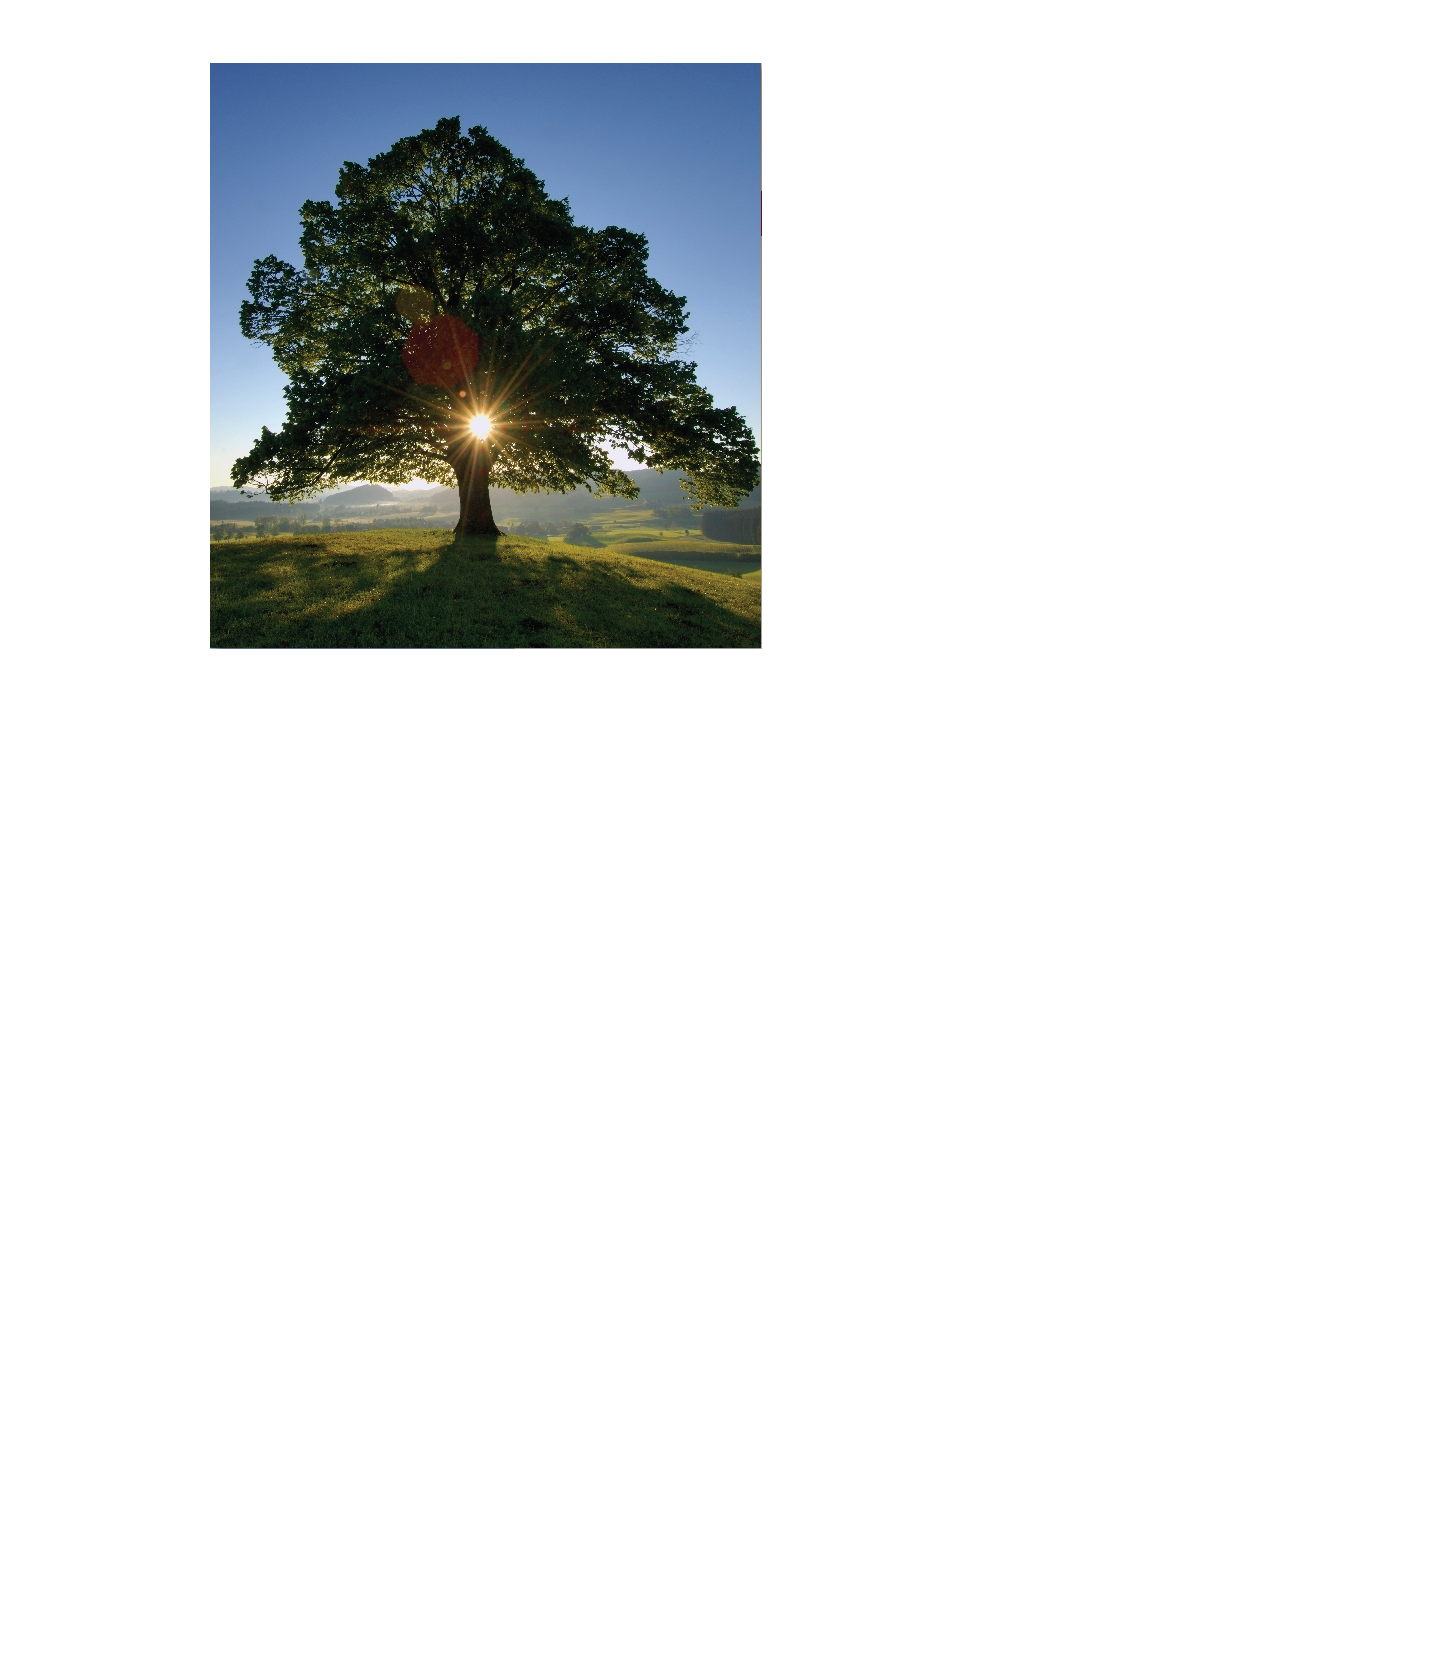
\includegraphics[width=0.6\linewidth]{images/fig1}
%
\par
You may have heard that mathematics is the language of science.  In fact, professionals in nearly every discipline take advantage of mathematical methods to analyze data, identify trends, and predict the effects of change.  This process is called \terminology{mathematical modeling}.  A model is a simplified representation of reality that helps us understand a process or phenomenon.  Because it is a simplification, a model can never be completely accurate.  Instead, it should focus on those aspects of the real situation that will help us answer specific questions. Here is an example.%
\par
The world's population is growing at different rates in different nations.  Many factors, including economic and social forces, influence the birth rate.  Is there a connection between birth rates and education levels?  The figure shows the birth rate plotted against the female literacy rate in 148 countries.  Although the data points do not all lie precisely on a line, we see a generally decreasing trend:  the higher the literacy rate, the lower the birth rate.  The \terminology{regression line} provides a model for this trend, and a tool for analyzing the data.  In this chapter we study the properties of linear models and some techniques for fitting a linear model to data.%
\begin{figure}
\centering
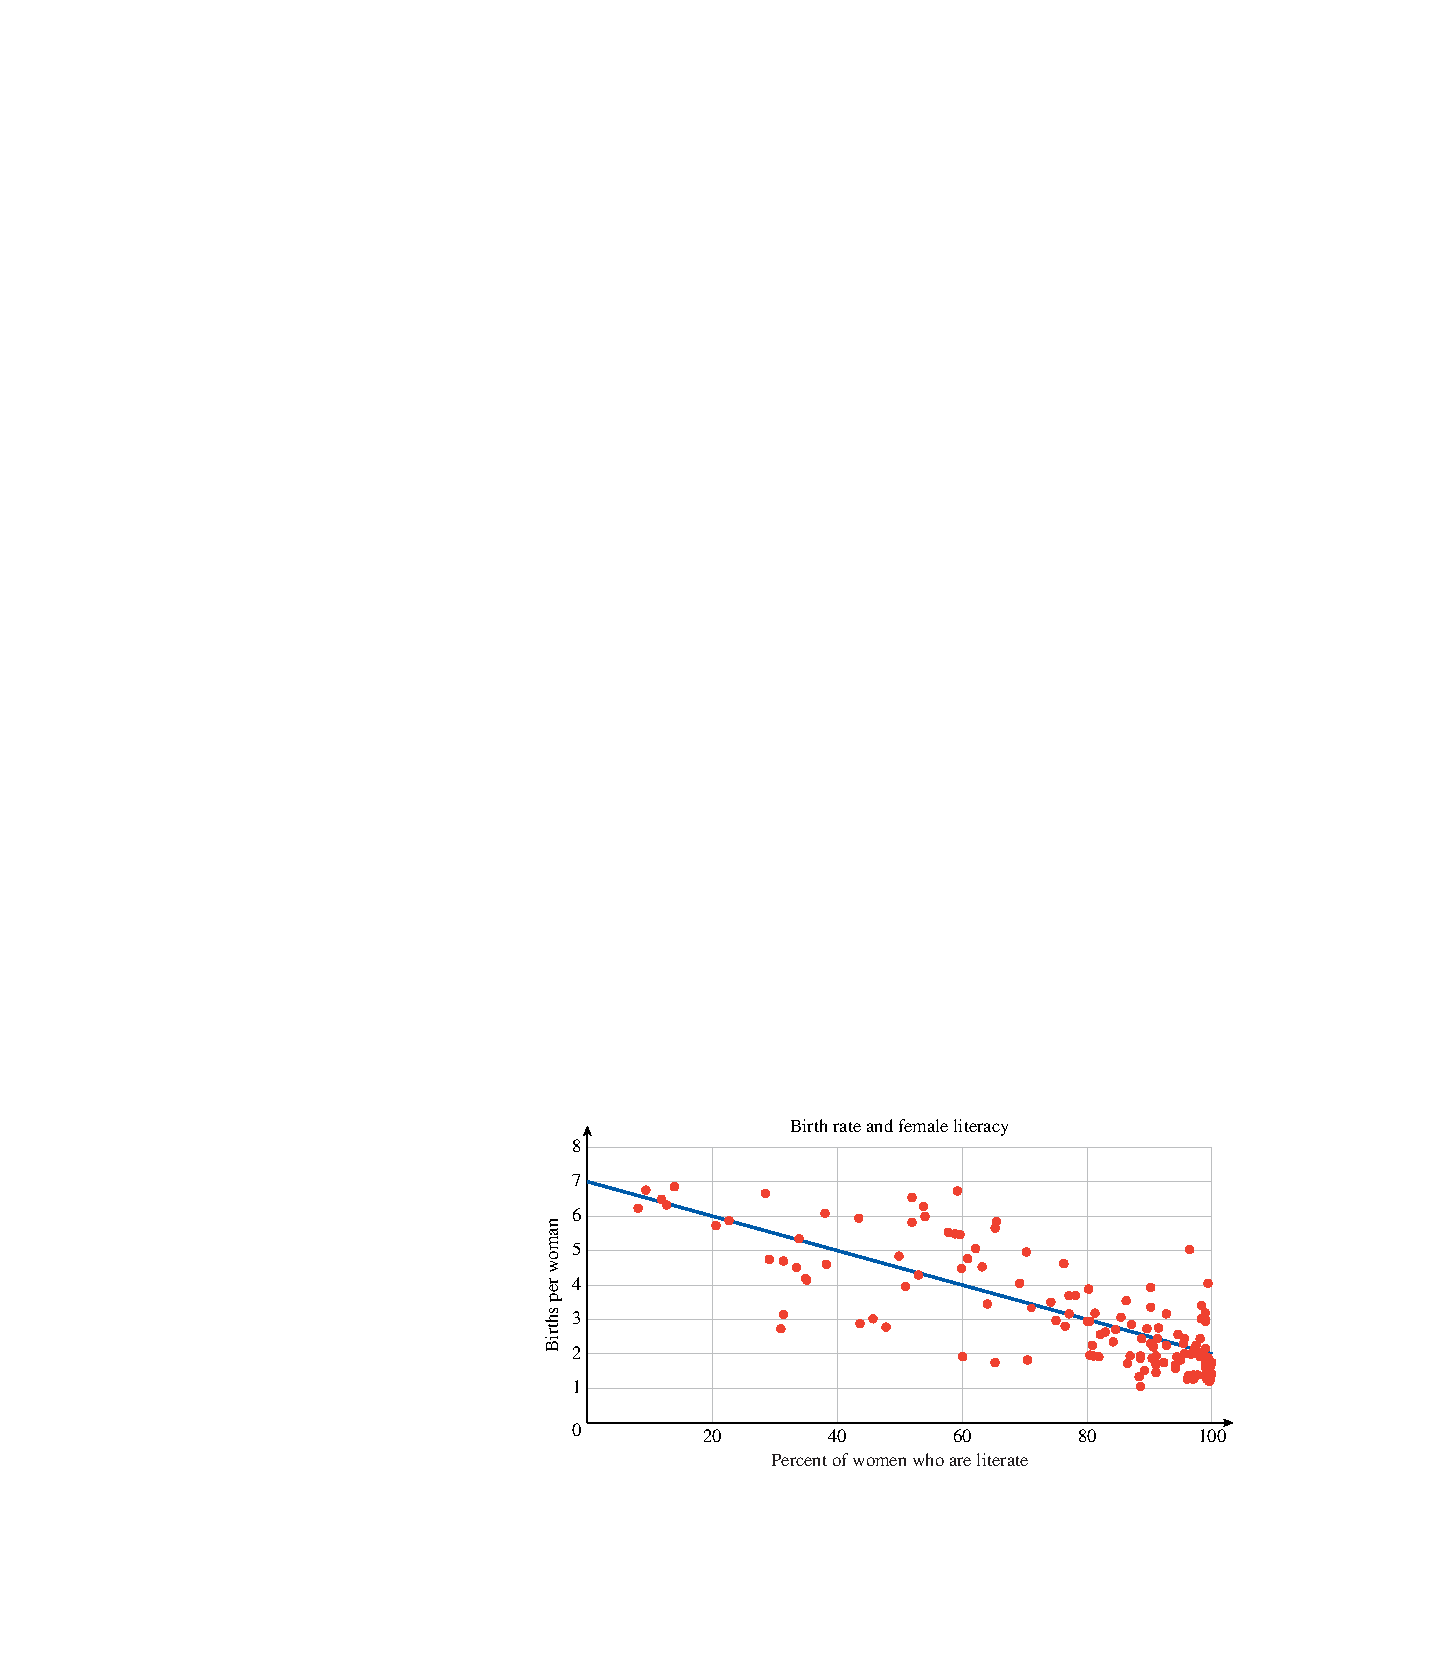
\includegraphics[width=1\linewidth]{images/BirthRateVsFemaleLiteracy}
\end{figure}
\begin{investigation}[Sales on Commission]\label{investigation-commission}
Delbert is offered a part-time job selling restaurant equipment. He will be paid \textdollar{}1000 per month plus a 6\% commission on his sales. The sales manager tells Delbert he can expect to sell about \textdollar{}8000 worth of equipment per month. To help him decide whether to accept the job, Delbert does a few calculations.%
\par
\leavevmode%
\begin{enumerate}
\item\hypertarget{li-1}{}Based on the sales manager’s estimate, what monthly income can Delbert expect from this job? What annual salary would that provide?%
\item\hypertarget{li-2}{}What would Delbert’s monthly salary be if he sold only \textdollar{}5000 of equipment per month? What would his salary be if he sold \textdollar{}10,000 worth per month? Compute monthly incomes for each sales total shown in the table.%
% group protects changes to lengths, releases boxes (?)
{% begin: group for a single side-by-side
% set panel max height to practical minimum, created in preamble
\setlength{\panelmax}{0pt}
\newsavebox{\panelboxAtabular}
\savebox{\panelboxAtabular}{%
\raisebox{\depth}{\parbox{0.5\textwidth}{\centering\begin{tabular}{AcAcA}\hrulethick
Sales&Income\tabularnewline\hrulethin
5000&\tabularnewline\hrulethin
8000&\tabularnewline\hrulethin
10,000&\tabularnewline\hrulethin
12,000&\tabularnewline\hrulethin
15,000&\tabularnewline\hrulethin
18,000&\tabularnewline\hrulethin
20,000&\tabularnewline\hrulethin
25,000&\tabularnewline\hrulethin
30,000&\tabularnewline\hrulethin
35,000&\tabularnewline\hrulethin
~&\tabularnewline\hrulethin
~&\tabularnewline\hrulethin
\end{tabular}
}}}
\newlength{\phAtabular}\setlength{\phAtabular}{\ht\panelboxAtabular+\dp\panelboxAtabular}
\settototalheight{\phAtabular}{\usebox{\panelboxAtabular}}
\setlength{\panelmax}{\maxof{\panelmax}{\phAtabular}}
\newsavebox{\panelboxCimage}
\savebox{\panelboxCimage}{%
\includegraphics[width=0.5\linewidth]{images/Investigation1Grid}
}
\newlength{\phCimage}\setlength{\phCimage}{\ht\panelboxCimage+\dp\panelboxCimage}
\settototalheight{\phCimage}{\usebox{\panelboxCimage}}
\setlength{\panelmax}{\maxof{\panelmax}{\phCimage}}
\leavevmode%
% begin: side-by-side as figure/tabular
% \tabcolsep change local to group
\setlength{\tabcolsep}{0\textwidth}
% @{} suppress \tabcolsep at extremes, so margins behave as intended
\begin{figure}
\begin{tabular}{@{}*{2}{c}@{}}
\begin{minipage}[c][\panelmax][t]{0.5\textwidth}\usebox{\panelboxAtabular}\end{minipage}&
\begin{minipage}[c][\panelmax][t]{0.5\textwidth}\usebox{\panelboxCimage}\end{minipage}\end{tabular}
\end{figure}
% end: side-by-side as tabular/figure
}% end: group for a single side-by-side
\item\hypertarget{li-3}{}Plot your data points on a graph, using sales, \(S\), on the horizontal axis and income, \(I\), on the vertical axis, as shown in the figure. Connect the data points to show Delbert’s monthly income for all possible monthly sales totals.%
\item\hypertarget{li-4}{}Add two new data points to the table by reading values from your graph.%
\item\hypertarget{li-5}{}Write an algebraic expression for Delbert’s monthly income, \(I\), in terms of his monthly sales, \(S\). Use the description in the problem to help you:%
\par
He will be paid: \textdollar{}1000 . . . plus a 6\% commission on his sales.%
\par
\emph{Income} \(= \fillin{6.818181818181818}\)%
\item\hypertarget{li-6}{}Test your formula from part (5) to see if it gives the same results as those you recorded in the table.%
\item\hypertarget{li-7}{}Use your formula to find out what monthly sales total Delbert would need in order to have a monthly income of \textdollar{}2500.%
\item\hypertarget{li-8}{}Each increase of \textdollar{}1000 in monthly sales increases Delbert’s monthly income by \fillin{6.818181818181818}.%
\item\hypertarget{li-9}{}Summarize the results of your work: In your own words, describe the relationship between Delbert’s monthly sales and his monthly income. Include in your discussion a description of your graph.%
\end{enumerate}
%
\end{investigation}
\typeout{************************************************}
\typeout{Section 1.1 Linear Models}
\typeout{************************************************}
\section[{Linear Models}]{Linear Models}\label{LinMod}
\typeout{************************************************}
\typeout{Subsection 1.1.1 Tables, Graphs and Equations}
\typeout{************************************************}
\subsection[{Tables, Graphs and Equations}]{Tables, Graphs and Equations}\label{subsection-1}
The first step in creating a model is to describe relationships between variables.  In \hyperref[investigation-commission]{Investigation~\ref{investigation-commission}}, we analyzed the relationship between Delbert's sales and his income.  Starting from the verbal description of his income, we represented the relationship by a table of values, a graph, and an algebraic equation.  Each of these mathematical tools is useful in a different way.%
\leavevmode%
\begin{enumerate}
\item\hypertarget{li-10}{}A \terminology{table of values} displays specific data points with precise numerical values.%
\item\hypertarget{li-11}{}A \terminology{graph} is a visual display of the data.  It is easier to spot trends and describe the overall behavior of the variables from a graph.%
\item\hypertarget{li-12}{}An \terminology{algebraic equation} is a compact summary of the model.  It can be used to analyze the model and to make predictions%
\end{enumerate}
We begin our study of modeling with some examples of \terminology{linear models}.  In the examples that follow, observe the interplay among the three modeling tools, and how each contributes to the model.%
\begin{example}[]\label{example-Annelise}
Annelise is on vacation at a seaside resort.  She can rent a bicycle from her hotel for \textdollar{}3 an hour, plus a \textdollar{}5 insurance fee.  (A fraction of an hour is charged as the same fraction of \textdollar{}3.)%
\leavevmode%
\begin{enumerate}[label=\alph*]
\item\hypertarget{li-13}{}Make a table of values showing the cost, \(C\), of renting a bike for various lengths of time, \(t\).%
\item\hypertarget{li-14}{}Plot the points on a graph.  Draw a curve through the data points%
. \item\hypertarget{li-15}{}Write an equation for \(C\) in terms of \(t\).%
\end{enumerate}
\par\medskip\noindent%
\textbf{Solution.}\quad \leavevmode%
\begin{enumerate}[label=\alph*]
\item\hypertarget{li-16}{}To find the cost, we multiply the time by \textdollar{}3, and add the result to the \textdollar{}5 insurance fee.  For example, the cost of a 1-hour bike ride is%
\begin{align*}
\text{Cost}\amp=(\$5\text{ insurance fee})+(\$3\text{ per hour})\times(\alert{1}\text{ hour})\\
C\amp=5+3(\alert{1})=8
\end{align*}
A 1-hour bike ride costs \textdollar{}8.  Record the results in a table, as shown here:%
\begin{table}
\centering
\begin{tabular}{AcAcAcAcA}\hrulethick
Length of rental (hours)&Cost of rental (dollars)&&\((t,C)\)\tabularnewline\hrulethin
\(1\)&\(8\)&\(C=5+3(\alert{1})\)&\((1,8)\)\tabularnewline\hrulethin
\(2\)&\(11\)&\(C=5+3(\alert{2})\)&\((2,11)\)\tabularnewline\hrulethin
\(3\)&\(14\)&\(C=5+3(\alert{3})\)&\((3,14)\)\tabularnewline\hrulethin
\end{tabular}
\end{table}
\item\hypertarget{li-17}{}Each pair of values represents a point on the graph.  The first value gives the horizontal coordinate of the point, and the second value gives the vertical coordinate.  The points lie on a straight line, as shown in the figure.  The line extends infinitely in only one direction, because negative values of \(t\) do not make sense here.%
\begin{figure}
\centering
\includegraphics[width=0.4\linewidth]{images/fig-Annelise-1}
\end{figure}
\item\hypertarget{li-18}{}To write an equation, let \(C\) represent the cost of the rental, and use \(t\) for the number of hours:%
\par
%
\begin{align*}
\text{Cost}\amp=(\$5\text{ insurance fee})+(\$3\text{ per hour})\times\text{(number of hours)}\\
C\amp=5+3\cdot t=8
\end{align*}
%
\end{enumerate}
%
\end{example}
\begin{example}[]\label{example-6hrbike}
Use the equation \(C=5+3\cdot t\) you found in \hyperref[example-Annelise]{Example~\ref{example-Annelise}} to answer the following questions.  Then show how to find the answers by using the graph.%
\leavevmode%
\begin{enumerate}[label=\alph*]
\item\hypertarget{li-19}{}How much will it cost Annelise to rent a bicycle for 6 hours?%
\item\hypertarget{li-20}{}How long can Annelise bicycle for \textdollar{}18.50?%
\end{enumerate}
\par\medskip\noindent%
\textbf{Solution.}\quad \leavevmode%
\begin{enumerate}[label=\alph*]
\item\hypertarget{li-21}{}Substitute \(t=\alert{6}\) into the expression for \(C\) to find%
\begin{equation*}
C=5+3(\alert{6})=23
\end{equation*}
A 6-hour bike ride will cost \textdollar{}23.  The point \(P\) on the graph in the figure represents the cost of a 6-hour bike ride.  The value on the \(C\)-axis at the same height as point \(P\) is 23, so a 6-hour bike ride costs \textdollar{}23.%
\item\hypertarget{li-22}{}Substitute \(C=\alert{18.50}\) into the equation and solve for \(t\).%
\begin{align*}
\alert{18.50}\amp=5+3t\\
13.50\amp=3t\\
t\amp=4.5
\end{align*}
For \textdollar{}18.50 Annelise can bicycle for 4½ hours. The point \(Q\)  on the graph represents an \textdollar{}18.50 bike ride.  The value on the \(t\)-axis below point \(Q\) is 4.5, so \textdollar{}18.50 will buy a 4.5 hour bike ride.%
\end{enumerate}
 \begin{figure}
\centering
\includegraphics[width=0.4\linewidth]{images/fig1-2}
\end{figure}
%
\end{example}
In \hyperref[example-6hrbike]{Example~\ref{example-6hrbike}}, notice the different algebraic techniques we used in parts (a) and (b).   In part (a), we were given a value of \(t\) and we \terminology{evaluated the expression}  \(5+3t\) to find \(C\).  In part (b) we were given a value of \(C\) and we \terminology{solved the equation} \(C=5+3t\) to find \(t\).%
\begin{exercise}\label{exercise-Frank-plants}
Frank plants a dozen corn seedlings, each 6 inches tall.  With plenty of water and sunlight they will grow approximately 2 inches per day.  Complete the table of values for the height, \(h\), of the seedlings after \(t\) days.%
% group protects changes to lengths, releases boxes (?)
{% begin: group for a single side-by-side
% set panel max height to practical minimum, created in preamble
\setlength{\panelmax}{0pt}
\newsavebox{\panelboxCtabular}
\savebox{\panelboxCtabular}{%
\raisebox{\depth}{\parbox{0.5\textwidth}{\centering\begin{tabular}{AcAcAcAcAcAcA}\hrulethick
\(t\)&\(0\)&\(5\)&\(10\)&\(15\)&\(20\)\tabularnewline\hrulethin
\(h\)&&&&&\tabularnewline\hrulethin
\end{tabular}
}}}
\newlength{\phCtabular}\setlength{\phCtabular}{\ht\panelboxCtabular+\dp\panelboxCtabular}
\settototalheight{\phCtabular}{\usebox{\panelboxCtabular}}
\setlength{\panelmax}{\maxof{\panelmax}{\phCtabular}}
\newsavebox{\panelboxFimage}
\savebox{\panelboxFimage}{%
\includegraphics[width=0.5\linewidth]{images/fig-Example2}
}
\newlength{\phFimage}\setlength{\phFimage}{\ht\panelboxFimage+\dp\panelboxFimage}
\settototalheight{\phFimage}{\usebox{\panelboxFimage}}
\setlength{\panelmax}{\maxof{\panelmax}{\phFimage}}
\leavevmode%
% begin: side-by-side as figure/tabular
% \tabcolsep change local to group
\setlength{\tabcolsep}{0\textwidth}
% @{} suppress \tabcolsep at extremes, so margins behave as intended
\begin{figure}
\begin{tabular}{@{}*{2}{c}@{}}
\begin{minipage}[c][\panelmax][t]{0.5\textwidth}\usebox{\panelboxCtabular}\end{minipage}&
\begin{minipage}[c][\panelmax][t]{0.5\textwidth}\usebox{\panelboxFimage}\end{minipage}\end{tabular}
\end{figure}
% end: side-by-side as tabular/figure
}% end: group for a single side-by-side
\leavevmode%
\begin{enumerate}[label=\alph*]
\item\hypertarget{li-23}{}Write an equation for the height of the seedlings in terms of the number of days since they were planted.%
\item\hypertarget{li-24}{}Graph the equation.%
\end{enumerate}
\end{exercise}
\begin{exercise}\label{exercise-2}
Use your equation from \hyperref[exercise-Frank-plants]{Exercise~\ref{exercise-Frank-plants}} to answer the questions.  Illustrate each answer on the graph.%
\leavevmode%
\begin{enumerate}[label=\alph*]
\item\hypertarget{li-27}{}How tall is the corn after 3 weeks?%
\item\hypertarget{li-28}{}How long will it be before the corn is 6 feet tall?%
\end{enumerate}
For part (b), convert feet to inches.%
\end{exercise}
\typeout{************************************************}
\typeout{Subsection 1.1.2 Choosing Scales for the Axes}
\typeout{************************************************}
\subsection[{Choosing Scales for the Axes}]{Choosing Scales for the Axes}\label{subsection-2}
To create a useful graph, we must choose appropriate scales for the axes.  The axes must extend far enough to show the values of the variables, and the tick marks should be equally spaced.  Usually we should use no more than 10 or 15 tick marks.%
\begin{example}[]\label{example-home-price}
In 1990, the median price of a home in the US was \textdollar{}92,000.  The median price increased by about \textdollar{}4700 per year over the next decade. \leavevmode%
\begin{enumerate}[label=\alph*]
\item\hypertarget{li-31}{}Make a table of values showing the median price of a house in 1990, 1994, 1998, and 2000.%
\item\hypertarget{li-32}{}Choose suitable scales for the axes and plot the values you found in part (a) on a graph. Use \(t\), the number of years since 1990, on the horizontal axis and the price of the house, \(P\), on the vertical axis.  Draw a curve through the points.%
\item\hypertarget{li-33}{}Write an equation that expresses \(P\) in terms of \(t\).%
\item\hypertarget{li-34}{}How much did the price of the house increase from 1990 to 1996?  Illustrate the increase on your graph.%
\end{enumerate}
%
\par\medskip\noindent%
\textbf{Solution.}\quad \leavevmode%
\begin{enumerate}[label=\alph*]
\item\hypertarget{li-35}{}In 1990 the median price was \textdollar{}92,000.  Four years later, in 1994, the price had increased by \(\alert{4}(4700)=18,800\) dollars, so%
\begin{equation*}
P=92,000+\alert{4}(4700)=110,800
\end{equation*}
In 1998 the price had increased by \(\alert{8}(4700)=37,600\)  dollars, so%
\begin{equation*}
P=92,000+\alert{8}(4700)=129,600
\end{equation*}
You can verify the price of the house in 2000 by a similar calculation.%
\begin{table}
\centering
\begin{tabular}{AcAcAcA}\hrulethick
Year&Price of House)&\((t,P)\)\tabularnewline\hrulethin
\(1990\)&\(92,000\)&\((0,\, 92,000)\)\tabularnewline\hrulethin
\(1994\)&\(110,800\)&\((4,\, 110,800)\)\tabularnewline\hrulethin
\(1998\)&\(129,600\)&\((8,\, 129,600)\)\tabularnewline\hrulethin
\(2000\)&\(139,000\)&\((10,\, 139,000)\)\tabularnewline\hrulethin
\end{tabular}
\end{table}
\item\hypertarget{li-36}{}Let \(t\) stand for the number of years since 1990, so that \(t=0\) in 1990, \(t=4\) in 1994, and so on.  To choose scales for the axes, look at the values in the table.  For this graph we scale the horizontal axis, or \(t\)-axis, in 1-year intervals and the vertical axis, or \(P\)-axis, for \textdollar{}90,000 to \textdollar{}140,000 in intervals of \textdollar{}5,000. The points in \hyperref[fig-median-house]{Figure~\ref{fig-median-house}}. lie on a straight line.%
\item\hypertarget{li-37}{}Look back at the calculations in part (a).  The price of the house started at \textdollar{}92,000 in 1990 and increased by \(t \times 4700\) dollars after \(t\) years.  Thus,%
\begin{equation*}
P=92,000+4700t
\end{equation*}
%
\item\hypertarget{li-38}{}Find the points on the graph corresponding to 1990 and 1996.%
\begin{figure}
\centering
\includegraphics[width=0.5\linewidth]{images/fig1-3}
\caption{\label{fig-median-house}}
\end{figure}
These points lie above \(t=0\) and \(t=6\) on the \(t\)-axis.  Now find the values on the \(P\)-axis corresponding to the two points.  The values are \(P=92,000\) in 1990 and \(P=120,200\) in 1996.  The increase in price is the difference of the two \(P\)-values.%
\begin{align*}
\text{increase in price}\amp=120,200-92,000
\\
\amp=28,200
\end{align*}
The price of the home increased \textdollar{}28,200 between 1990 and 1996.  This increase is indicated by the arrows in \hyperref[fig-median-house]{Figure~\ref{fig-median-house}}.%
\end{enumerate}
\end{example}
The graphs in the preceding examples are \terminology{increasing graphs}.  As we move along the graph from left to right (in the direction of increasing \(t\) ), the second coordinate increases as well.  Try \hyperref[exercise-Silver-Lake]{Exercise~\ref{exercise-Silver-Lake}}, which illustrates a \terminology{decreasing graph}.%
\begin{exercise}\label{exercise-Silver-Lake}
Silver Lake has been polluted by industrial waste products.  The concentration of toxic chemicals in the water is currently 285 parts per million (ppm).  Local environmental officials would like to reduce the concentration by 15 ppm each year%
\leavevmode%
\begin{enumerate}[label=\alph*]
\item\hypertarget{li-39}{}Complete the table of values showing the desired concentration, \(C,\)~ of toxic chemicals \(t\) years from now.  For each \(t\)-value, calculate the corresponding value for \(C\).  Write your answers as ordered pairs.%
\begin{table}
\centering
\begin{tabular}{AcAcAcAcA}\hrulethick
\(t\)&\(C\)&&\((t,C)\)\tabularnewline\hrulethin
\(0\)&&\(C=285-150(\alert{0})\)&\((0, ~~~~ )\)\tabularnewline\hrulethin
\(5\)&&\(C=285-150(\alert{5})\)&\((5, ~~~~ )\)\tabularnewline\hrulethin
\(10\)&&\(C=285-150(\alert{10})\)&\((10, ~~~~ )\)\tabularnewline\hrulethin
\(15\)&&\(C=285-150(\alert{15})\)&\((15, ~~~~ )\)\tabularnewline\hrulethin
\end{tabular}
\end{table}
\item\hypertarget{li-40}{}To choose scales for the axes, notice that the value of \(C\) starts at 285 and decreases from there.  We'll scale the vertical axis up to 300, and use 10 tick marks at intervals of 30.  Graph the ordered pairs on the grid, and connect them with a straight line. Extend the graph until it reaches the horizontal axis, but no farther.  Points with negative \(C\)-coordinates have no meaning for the problem.%
\item\hypertarget{li-41}{}Write an equation for the concentration, \(C\), of toxic chemicals \(t\) years from now.%
\includegraphics[width=0.5\linewidth]{images/fig-Exercise3}
\end{enumerate}
\par\smallskip
\noindent\textbf{Hint.}\hypertarget{hint-2}{}\quad
For part (c): The concentration is initially 8 ppm, and we subtract 15 ppm for each year that passes, or \(15 \times t\).%
\end{exercise}
\begin{remark}[Graphing an Equation]\label{remark-1}
We can use a graphing calculator to graph an equation. On most calculators, we follow three steps.%
\par
To Graph an Equation:%
\leavevmode%
\begin{enumerate}
\item\hypertarget{li-45}{}Press \lstinline?Y=? and enter the equation you wish to graph.%
\item\hypertarget{li-46}{}Press \lstinline?WINDOW? and select a suitable graphing window.%
\item\hypertarget{li-47}{}Press \lstinline?GRAPH?%
\end{enumerate}
\end{remark}
\begin{example}[Using a Graphing Calculator]\label{graphing-calculator}
In \hyperref[example-home-price]{Example~\ref{example-home-price}}, we found the equation \(P = 92,000 + 4700t\) for the median price of a house \(t\) years after 1990. Graph this equation on a calculator.%
\par\medskip\noindent%
\textbf{Solution.}\quad To begin, we press \lstinline?Y=? and enter%
\begin{equation*}
Y1 = 92,000 + 4700X
\end{equation*}
%
\par
For this graph, we’ll use the grid in \hyperref[example-home-price]{Example~\ref{example-home-price}} for our window settings, so we press \lstinline?WINDOW? and enter%
\begin{table}
\centering
\begin{tabular}{lll}
Xmin\(=0\)&&Xmax\(=10\)\tabularnewline[0pt]
Ymin\(=90,000\)&&Ymax\(=140,000\)
\end{tabular}
\end{table}
Finally, we press \lstinline?GRAPH?. The calculator's graph is shown in \hyperref[fig-GC-house-price]{Figure~\ref{fig-GC-house-price}}. \begin{figure}
\centering
\includegraphics[width=0.5\linewidth]{images/fig-GC-house-price}
\caption{\label{fig-GC-house-price}}
\end{figure}
%
\end{example}
\begin{exercise}\label{exercise-gc}
\leavevmode%
\begin{enumerate}[label=\alph*]
\item\hypertarget{li-48}{}Solve the equation \(2y - 1575 = 45x\) for \(y\) in terms of \(x\).%
\item\hypertarget{li-49}{}Graph the equation on a graphing calculator. Use the window \leavevmode%
\begin{table}
\centering
\begin{tabular}{lllll}
Xmin\(=-50\)&&Xmax\(=50\)&&Xscl\(=5\)\tabularnewline[0pt]
Ymin\(=-500\)&&Ymax\(=1000\)&&Yscl\(=100\)
\end{tabular}
\end{table}
%
\item\hypertarget{li-50}{}Sketch the graph on paper. Use the window settings to choose appropriate scales for the axes.%
\end{enumerate}
\end{exercise}
\typeout{************************************************}
\typeout{Subsection 1.1.3 Linear Equations}
\typeout{************************************************}
\subsection[{Linear Equations}]{Linear Equations}\label{subsection-3}
All the models in the preceding examples have equations with a similar form:%
\begin{equation*}
y=\text{(starting value)}+\text{(rate of change)}\cdot x
\end{equation*}
(We'll talk more about rate of change in \hyperref[slope-and-rate-of-change]{Section~\ref{slope-and-rate-of-change}}.)  Their graphs were all portions of straight lines.  For this reason such equations are called  \terminology{linear equations}.  The order of the terms in the equation does not matter.  For example, the equation in \hyperref[example-Annelise]{Example~\ref{example-Annelise}},%
\begin{equation*}
C=5+3t
\end{equation*}
can be written equivalently as%
\begin{equation*}
-3t+C=5
\end{equation*}
and the equation in \hyperref[example-home-price]{Example~\ref{example-home-price}},%
\begin{equation*}
P=92,000+4700t
\end{equation*}
can be written as%
\begin{equation*}
-4700t +P=92,000
\end{equation*}
This form of a linear equation,%
\begin{equation*}
Ax+By=C
\end{equation*}
is called the \terminology{general form}.%
\begin{assemblage}{General Form for a Linear Equation}\label{assemblage-1}
The graph of any equation%
\begin{equation*}
Ax+By=C
\end{equation*}
where \(A\) and \(B\) are not both equal to zero, is a straight line.%
\end{assemblage}
\begin{example}[]\label{example-advertising}
The manager at Albert's Appliances has \textdollar{}3000 to spend on advertising for the next fiscal quarter.  A 30-second spot on television costs \textdollar{}150 per broadcast, and a 30-second radio ad costs \textdollar{}50.%
\leavevmode%
\begin{enumerate}[label=\alph*]
\item\hypertarget{li-54}{}The manager decides to buy \(x\) television ads and \(y\) radio ads.  Write an equation relating \(x\) and \(y\).%
\item\hypertarget{li-55}{}Make a table of values showing several choices for \(x\) and \(y\).%
\item\hypertarget{li-56}{}Plot the points from your table, and graph the equation.%
\end{enumerate}
\par\medskip\noindent%
\textbf{Solution.}\quad \leavevmode%
\begin{enumerate}[label=\alph*]
\item\hypertarget{li-57}{}Each television ad costs \textdollar{}150, so \(x\) ads will cost \(\$150x\).  Similarly, \(y\) radio ads will cost \(\$50y\).  The manager has \textdollar{}3000 to spend, so the sum of the costs must be \textdollar{}3000.  Thus,%
\begin{equation*}
150x+50y=3000
\end{equation*}
%
\item\hypertarget{li-58}{}Choose some values of \(x\), and solve the equation for the corresponding value of \(y\).  For example, if \(x=\alert{10}\) then%
\begin{align*}
150(\alert{10})+50y\amp=300\\
1500+50y\amp=3000\\
50y\amp=1500\\
y\amp=30
\end{align*}
If the manager buys 10 television ads, she can also buy 30 radio ads.  You can verify the other entries in the table.%
\begin{table}
\centering
\begin{tabular}{AcAcAcAcAcA}\hrulethick
\(x\)&\(8\)&\(10\)&\(12\)&\(14\)\tabularnewline\hrulethin
\(y\)&\(36\)&\(30\)&\(24\)&\(18\)\tabularnewline\hrulethin
\end{tabular}
\end{table}
\item\hypertarget{li-59}{}Plot the points from the table.  All the solutions lie on a straight line, as shown in \hyperref[fig-example-advertising]{Figure~\ref{fig-example-advertising}} . \begin{figure}
\centering
\includegraphics[width=0.4\linewidth]{images/fig-example-advertising}
\caption{\label{fig-example-advertising}}
\end{figure}
%
\end{enumerate}
%
\end{example}
\begin{exercise}\label{exercise-crops}
In central Nebraska, each acre of corn requires 25 acre-inches of water per year, and each acre of winter wheat requires 18 acre-inches of water.             (An acre-inch is the amount of water needed to cover one acre of land to a depth of one inch.)  A farmer can count on 9000 acre-inches of water for the coming year.  (Source:  Institute of Agriculture and Natural Resources, University of Nebraska) \leavevmode%
\begin{enumerate}[label=\alph*]
\item\hypertarget{li-60}{}Write an equation relating the number of acres of corn, \(x\), and the number of acres of wheat, \(y\), that the farmer can plant.%
\item\hypertarget{li-61}{}Complete the table.%
\begin{table}
\centering
\begin{tabular}{AcAcAcAcAcA}\hrulethick
\(x\)&\(50\)&\(100\)&\(150\)&\(200\)\tabularnewline\hrulethin
\(y\)&\(\hphantom{0000}\)&\(\hphantom{0000}\)&\(\hphantom{0000}\)&\(\hphantom{0000}\)\tabularnewline\hrulethin
\end{tabular}
\end{table}
\end{enumerate}
%
\end{exercise}
\typeout{************************************************}
\typeout{Subsection 1.1.4 Intercepts}
\typeout{************************************************}
\subsection[{Intercepts}]{Intercepts}\label{subsection-4}
% group protects changes to lengths, releases boxes (?)
{% begin: group for a single side-by-side
% set panel max height to practical minimum, created in preamble
\setlength{\panelmax}{0pt}
\newsavebox{\panelboxOimage}
\savebox{\panelboxOimage}{%
\includegraphics[width=0.35\linewidth]{images/fig-intercepts}
}
\newlength{\phOimage}\setlength{\phOimage}{\ht\panelboxOimage+\dp\panelboxOimage}
\settototalheight{\phOimage}{\usebox{\panelboxOimage}}
\setlength{\panelmax}{\maxof{\panelmax}{\phOimage}}
\newsavebox{\panelboxDKp}
\savebox{\panelboxDKp}{%
\raisebox{\depth}{\parbox{0.6\textwidth}{Consider the graph of the equation%
\begin{equation*}
3x-4y=12
\end{equation*}
shown in \hyperref[fig-intercepts]{Figure~\ref{fig-intercepts}}. The points where the graph crosses the axes are called the \terminology{intercepts} of the graph. The coordinates of these points are easy to find.  The \(y\)-coordinate of the \(x\)-intercept is zero, so we set \(y=\alert{0}\) in the equation to get%
\begin{align*}
3(\alert{0})-4x\amp=12\\
x=-3
\end{align*}
}}}
\newlength{\phDKp}\setlength{\phDKp}{\ht\panelboxDKp+\dp\panelboxDKp}
\settototalheight{\phDKp}{\usebox{\panelboxDKp}}
\setlength{\panelmax}{\maxof{\panelmax}{\phDKp}}
\leavevmode%
% begin: side-by-side as figure/tabular
% \tabcolsep change local to group
\setlength{\tabcolsep}{0.025\textwidth}
% @{} suppress \tabcolsep at extremes, so margins behave as intended
\begin{figure}
\begin{tabular}{@{}*{2}{c}@{}}
\begin{minipage}[c][\panelmax][t]{0.35\textwidth}\usebox{\panelboxOimage}\end{minipage}&
\begin{minipage}[c][\panelmax][t]{0.6\textwidth}\usebox{\panelboxDKp}\end{minipage}\tabularnewline
\parbox[t]{0.35\textwidth}{\captionof{figure}{\label{fig-intercepts}}
}&
\end{tabular}
\end{figure}
% end: side-by-side as tabular/figure
}% end: group for a single side-by-side
The \(x\)-intercept is the point \((-3,0)\). Also, the \(x\)-coordinate of the \(y\)-intercept is zero, so we set \(x=\alert{0}\) in the equation to get%
\begin{gather*}
3y-4(\alert{0})=12\\
y=4
\end{gather*}
The \(y\)-intercept is \((0,4)\).%
\begin{assemblage}{Intercepts of a Graph}\label{assemblage-2}
The points where a graph crosses the axes are called the \terminology{intercepts of the graph}. \leavevmode%
\begin{enumerate}
\item\hypertarget{li-64}{}To find the \(y\)-intercept, set \(x=0\) and solve for \(y\).%
\item\hypertarget{li-65}{}To find the \(x\)-intercept, set \(y=0\) and solve for \(x\)%
\end{enumerate}
%
\end{assemblage}
The intercepts of a graph tell us something about the situation it models.%
\begin{example}[]\label{example-intercepts}
\leavevmode%
\begin{enumerate}[label=\alph*]
\item\hypertarget{li-66}{}Find the intercepts of the graph in \hyperref[exercise-Silver-Lake]{Exercise~\ref{exercise-Silver-Lake}}, about the pollution in Silver Lake.%
\item\hypertarget{li-67}{}What do the intercepts tell us about the problem?%
\end{enumerate}
\par\medskip\noindent%
\textbf{Solution.}\quad \leavevmode%
\begin{enumerate}[label=\alph*]
\item\hypertarget{li-68}{}An equation for the concentration of toxic chemicals is%
\begin{equation*}
C=285-15t
\end{equation*}
To find the \(C\)-intercept, set \(t\) equal to zero.%
\begin{equation*}
C=285-15(0)=285
\end{equation*}
The \(C\)-intercept is the point \((0, 285)\), or simply 285.  To find the \(t\)-intercept, set \(C\) equal to zero and solve for \(t\). \begin{align*} \alert{0}\&=285-15t \&\&\text{Add }15t \text{ to both sides.}\textbackslash{}\textbackslash{} 15t\&=285  \&\&\text{Divide both sides by 15.}\textbackslash{}\textbackslash{} t\&=19   \&\& \end{align*}%
 \par
The \(t\)-intercept is the point \((19,0)\), or simply \(19\).%
%
\item\hypertarget{li-69}{}The \(C\)-intercept represents the concentration of toxic chemicals in Silver Lake now:  When  \(t=0\), \(C=285\),  so the concentration is currently \(285\) ppm.  The \(t\)-intercept represents the number of years it will take for the concentration of toxic chemicals to drop to zero:  When \(C=0\), \(t=19\),  so it will take \(19\) years for the pollution to be eliminated entirely.%
\end{enumerate}
\end{example}
\begin{exercise}\label{exercise-6}
\leavevmode%
\begin{enumerate}[label=\alph*]
\item\hypertarget{li-70}{}Find the intercepts of the graph in \hyperref[example-advertising]{Example~\ref{example-advertising}}, about the advertising budget for Albert's Appliances: \(150x + 50y = 3000\).%
\item\hypertarget{li-71}{}What do the intercepts tell us about the problem?%
\end{enumerate}
\end{exercise}
\typeout{************************************************}
\typeout{Subsection 1.1.5 Intercept Method for Graphing Lines}
\typeout{************************************************}
\subsection[{Intercept Method for Graphing Lines}]{Intercept Method for Graphing Lines}\label{subsection-5}
Because we really only need two points to graph a linear equation, we might as well find the intercepts first and use them to draw the graph. The values of the intercepts will also help us choose suitable scales for the axes. It is always a good idea to find a third point as a check.%
\begin{example}[]\label{intercepts}
\leavevmode%
\begin{enumerate}[label=\alph*]
\item\hypertarget{li-72}{}Find the \(x\)- and \(y\)-intercepts of the graph of \(150x - 180y = 9000\).%
\item\hypertarget{li-73}{}Use the intercepts to graph the equation. Find a third point as a check.%
\end{enumerate}
\par\medskip\noindent%
\textbf{Solution.}\quad \leavevmode%
\begin{enumerate}[label=\alph*]
\item\hypertarget{li-74}{}To find the \(x\)-intercept, set \(y = \alert{0}\).%
\par
\begin{align*} 150x-18(\alert{0})\&=9000 \&\&\text{Simpify.}\textbackslash{}\textbackslash{} 150x\&=9000  \&\&\text{Divide both sides by 150.}\textbackslash{}\textbackslash{} x\&=60   \&\& \end{align*}%
\par
The \(x\)-intercept is the point \((60, 0)\). To find the \(y\)-intercept, set \(x = \alert{0}\).%
\par
\begin{align*} 150(\alert{0})-18y\&=9000 \&\&\text{Simpify.}\textbackslash{}\textbackslash{} -180y\&=9000  \&\&\text{Divide both sides by } -180\text{.}\textbackslash{}\textbackslash{} y\&=-50   \&\& \end{align*}%
\par
The \(y\)-intercept is the point \((0, -50)\).%
\item\hypertarget{li-75}{}Scale both axes in intervals of 10 and then plot the two intercepts, \((60, 0)\) and \((0, -50)\). Draw the line through them, as shown in \hyperref[fig-example-graph-intercepts]{Figure~\ref{fig-example-graph-intercepts}}. Now find another point and check that it lies on this line. We choose \(x = \alert{20}\) and solve for \(y\).%
\begin{align*}
150(\alert{20}) -180y \amp = 9000\\
3000 -180y \amp = 9000\\
-180y \amp = 6000\\
y \amp =-33.\overline{3}
\end{align*}
Plot the point \((20, -33\frac{1}{3})\). Because this point lies on the line, we can be reasonably confident that our graph is correct. \begin{figure}
\centering
\includegraphics[width=0.5\linewidth]{images/fig-example-graph-intercepts}
\caption{\label{fig-example-graph-intercepts}}
\end{figure}
%
\end{enumerate}
\end{example}
\begin{remark}[Choosing a Graphing Window]\label{remark-2}
Knowing the intercepts can also help us choose a suitable window on a graphing calculator. We would like the window to be large enough to show the intercepts. For the graph in \hyperref[fig-example-graph-intercepts]{Figure~\ref{fig-example-graph-intercepts}}, we can enter the equation%
\begin{equation*}
Y = (9000 -150X)/ -180
\end{equation*}
in the window \begin{table}
\centering
\begin{tabular}{lll}
Xmin\(=-20\)&&Xmax\(=70\)\tabularnewline[0pt]
Ymin\(=-70\)&&Ymax\(=30\)
\end{tabular}
\end{table}
%
\end{remark}
\begin{assemblage}{To Graph a Line Using the Intercept Method:}\label{assemblage-3}
\leavevmode%
\begin{enumerate}[label=*\arabic**]
\item\hypertarget{li-76}{}Find the intercepts of the line.%
%
\begin{enumerate}[label=++\alph*]
\item\hypertarget{li-77}{}To find the \(x\)-intercept, set \(y=0\) and solve for \(x\).%
\item\hypertarget{li-78}{}To find the \(y\)-intercept, set \(x = 0\) and solve for \(y\).%
\end{enumerate}
\item\hypertarget{li-79}{}Plot the intercepts.%
\item\hypertarget{li-80}{}Choose a value for \(x\) and find a third point on the line.%
\item\hypertarget{li-81}{}Draw a line through the points.%
\end{enumerate}
%
\end{assemblage}
\begin{exercise}\label{exercise-intercepts}
\leavevmode%
\begin{enumerate}[label=\alph*]
\item\hypertarget{li-82}{}In \hyperref[exercise-crops]{Exercise~\ref{exercise-crops}}, you wrote an equation about crops in Nebraska. Find the intercepts of the graph.%
\item\hypertarget{li-83}{}Use the intercepts to help you choose appropriate scales for the axes, and then graph the equation.%
\item\hypertarget{li-84}{}What do the intercepts tell us about the problem?%
\end{enumerate}
\end{exercise}
The examples in this section model simple linear relationships between two variables. Such relationships, in which the value of one variable is determined by the value of the other, are called \terminology{functions}. We will study various kinds of functions throughout the course.%
\typeout{************************************************}
\typeout{Subsection 1.1.6 Section Summary}
\typeout{************************************************}
\subsection[{Section Summary}]{Section Summary}\label{summary-1-1}
\typeout{************************************************}
\typeout{Subsubsection 1.1.6.1 Vocabulary}
\typeout{************************************************}
\subsubsection[{Vocabulary}]{Vocabulary}\label{subsubsection-1}
Look up the definitions of new terms in the Glossary. \leavevmode%
\begin{multicols}{3}
\begin{itemize}[label=\textbullet]
\item{}Variable%
\item{}Mathematical model%
\item{}Increasing graph%
\item{}Linear equation%
\item{}Solve an equation%
\item{}Evaluate an expression%
\item{}Intercept%
\item{}Decreasing graph%
\end{itemize}
\end{multicols}
%
\typeout{************************************************}
\typeout{Subsubsection 1.1.6.2 CONCEPTS}
\typeout{************************************************}
\subsubsection[{CONCEPTS}]{CONCEPTS}\label{subsubsection-2}
\leavevmode%
\begin{enumerate}[label=\arabic*]
\item\hypertarget{li-93}{}We can describe a relationship between variables with a table of values, a graph, or an equation.%
\item\hypertarget{li-94}{}Linear models have equations of the following form:%
\begin{equation*}
y = (\text{starting value}) + (\text{rate of change})\cdot x
\end{equation*}
%
\item\hypertarget{li-95}{}To make a useful graph, we must choose appropriate scales for the axes.%
\item\hypertarget{li-96}{}\begin{assemblage}{General Form for a Linear Equation}\label{assemblage-4}
The graph of any equation%
\begin{equation*}
Ax+By=C
\end{equation*}
where \(A\) and \(B\) are not both equal to zero, is a straight line.%
\end{assemblage}
%
\item\hypertarget{li-97}{}The intercepts of a graph are the points where the graph crosses the axes.%
\item\hypertarget{li-98}{}We can use the intercepts to graph a line.%
\begin{assemblage}{To Graph a Line Using the Intercept Method:}\label{assemblage-5}
%
\begin{enumerate}[label=\arabic*]
\item\hypertarget{li-99}{}Find the intercepts of the line.%
%
\begin{enumerate}[label=++\alph*]
\item\hypertarget{li-100}{}To find the \(x\)-intercept, set \(y=0\) and solve for \(x\).%
\item\hypertarget{li-101}{}To find the \(y\)-intercept, set \(x = 0\) and solve for \(y\).%
\end{enumerate}
\item\hypertarget{li-102}{}Plot the intercepts.%
\item\hypertarget{li-103}{}Choose a value for \(x\) and find a third point on the line.%
\item\hypertarget{li-104}{}Draw a line through the points.%
\end{enumerate}
%
\end{assemblage}
\item\hypertarget{li-105}{}The intercepts are also useful for interpreting a model.%
\end{enumerate}
%
\typeout{************************************************}
\typeout{Subsubsection 1.1.6.3 STUDY QUESTIONS}
\typeout{************************************************}
\subsubsection[{STUDY QUESTIONS}]{STUDY QUESTIONS}\label{subsubsection-3}
\leavevmode%
\begin{enumerate}[label=\arabic*]
\item\hypertarget{li-106}{}Name three ways to represent a relationship between two variables.%
\item\hypertarget{li-107}{}If \(C\) is expressed in terms of \(H\), which variable goes on the horizontal axis?%
\item\hypertarget{li-108}{}Explain the difference between evaluating an expression and solving an equation.%
\item\hypertarget{li-109}{}How many points do you need to graph a linear equation?%
\item\hypertarget{li-110}{}Explain how the words \terminology{intercept} and \terminology{intersect} are related; explain how they are different.%
\item\hypertarget{li-111}{}Delbert says that the intercepts of the line \(3x + 5y = 30\) are \((10, 6)\). What is wrong with his answer?%
\end{enumerate}
%
\typeout{************************************************}
\typeout{Subsubsection 1.1.6.4 SKILLS}
\typeout{************************************************}
\subsubsection[{SKILLS}]{SKILLS}\label{subsubsection-4}
Practice each skill in the \hyperref[section-1-1-exercises]{Homework~\ref{section-1-1-exercises}} problems listed. \leavevmode%
\begin{enumerate}[label=\arabic*]
\item\hypertarget{li-112}{}Make a table of values: \#1\textendash{}4, 7 and 8%
\item\hypertarget{li-113}{}Plot points and draw a graph: \#1– 4, 7 and 8%
\item\hypertarget{li-114}{}Choose appropriate scales for the axes: \#5\textendash{}12%
\item\hypertarget{li-115}{}Write a linear model of the form \(y = (\text{starting value}) + (\text{rate of change})\cdot x\): \#1\textendash{}8%
\item\hypertarget{li-116}{}Write a linear model in general form: \#25\textendash{}28, 33\textendash{}36%
\item\hypertarget{li-117}{}Evaluate a linear expression, algebraically and graphically: \#1\textendash{}4%
\item\hypertarget{li-118}{}Solve a linear equation, algebraically and graphically: \#1\textendash{}4%
\item\hypertarget{li-119}{}Find the intercepts of a graph: \#5 and 6, 13–24, 45–52%
\item\hypertarget{li-120}{}Graph a line by the intercept method: \#5 and 6, 13–24%
\item\hypertarget{li-121}{}Interpret the meaning of the intercepts: \#5 and 6, 25–28%
\item\hypertarget{li-122}{}Use a graphing calculator to graph a line: \#37\textendash{}52%
\item\hypertarget{li-123}{}Sketch on paper a graph obtained on a calculator: \#37\textendash{}44%
\end{enumerate}
%
\typeout{************************************************}
\typeout{Exercises 1.1.7 Homework}
\typeout{************************************************}
\subsection[{Homework}]{Homework}\label{section-1-1-exercises}
\begin{exerciselist}
\item[1.]\hypertarget{exercise-8}{}The temperature in the desert at 6 a.m., just before sunrise, was \(65\degree\)F. The temperature rose \(5\) degrees every hour until it reached its maximum value at about 5 p.m. Complete the table of values for the temperature, \(T\), at \(h\) hours after 6 a.m. \begin{table}
\centering
\begin{tabular}{AcAcAcAcAcAcA}\hrulethick
\(h\)&\(0\)&\(3\)&\(6\)&\(9\)&\(10\)\tabularnewline\hrulethin
\(T\)&\(\hphantom{0000}\)&\(\hphantom{0000}\)&\(\hphantom{0000}\)&\(\hphantom{0000}\)&\(\hphantom{0000}\)\tabularnewline\hrulethin
\end{tabular}
\end{table}
 \leavevmode%
\begin{enumerate}[label=\alph*]
\item\hypertarget{li-124}{}Write an equation for the temperature, \(T\), in terms of \(h\).%
\item\hypertarget{li-125}{}Graph the equation. \includegraphics[width=0.5\linewidth]{images/fig-ex-1-1-1}
%
\item\hypertarget{li-126}{}How hot is it at noon? Illustrate the answer on your graph.%
\item\hypertarget{li-127}{}When will the temperature be \(110\degree\)F? Illustrate the answer on your graph.%
\end{enumerate}
%
\par\smallskip
\par\smallskip
\noindent\textbf{Answer.}\hypertarget{answer-8}{}\quad
\begin{tabular}{AcAcAcAcAcAcA}\hrulethick
\(h\)&\(0\)&\(3\)&\(6\)&\(9\)&\(10\)\tabularnewline\hrulethin
\(T\)&\(65\)&\(80\)&\(95\)&\(110\)&\(115\)\tabularnewline\hrulethin
\end{tabular}
 \leavevmode%
\begin{enumerate}[label=\alph*]
\item\hypertarget{li-128}{}\(T=65+5h\)%
\item\hypertarget{li-129}{}\includegraphics[width=0.5\linewidth]{images/fig-ans-1-1-1}
%
\item\hypertarget{li-130}{}\(95\degree\)%
\item\hypertarget{li-131}{}3 p.m.%
\end{enumerate}
%
\item[2.]\hypertarget{exercise-9}{}The taxi out of Dulles Airport charges a traveler with one suitcase an initial fee of \(\$2.00\), plus \(\$1.50\) for each mile traveled. Complete the table of values showing the charge, \(C\), for a trip of \(n\) miles. \begin{table}
\centering
\begin{tabular}{AcAcAcAcAcAcAcA}\hrulethick
\(n\)&\(0\)&\(5\)&\(10\)&\(15\)&\(20\)&\(25\)\tabularnewline\hrulethin
\(C\)&\(\hphantom{0000}\)&\(\hphantom{0000}\)&\(\hphantom{0000}\)&\(\hphantom{0000}\)&\(\hphantom{0000}\)&\(\hphantom{0000}\)\tabularnewline\hrulethin
\end{tabular}
\end{table}
 \leavevmode%
\begin{enumerate}[label=(\alph*)]
\item\hypertarget{li-132}{}Write an equation for the charge, \(C\), in terms of the number of miles traveled, \(n\).%
\item\hypertarget{li-133}{}Graph the equation. \includegraphics[width=0.5\linewidth]{images/fig-ex-1-1-2}
%
\item\hypertarget{li-134}{}What is the charge for a trip to Mount Vernon,  \(40\) miles from the airport? Illustrate the answer on your graph.%
\item\hypertarget{li-135}{}If a ride to the National Institutes of Health (NIH) costs \(\$39.50\), how far is it from the airport to the NIH? Illustrate the answer on your graph.%
\end{enumerate}
%
\par\smallskip
\item[3.]\hypertarget{exercise-10}{}On October 31, Betty and Paul fill their \(250\)-gallon oil tank for their heater. Beginning in November, they use an average of \(15\) gallons of oil per week. Complete the table of values for the amount of oil, \(A\), left in the tank after \(w\) weeks. \begin{table}
\centering
\begin{tabular}{AcAcAcAcAcAcA}\hrulethick
\(w\)&\(0\)&\(4\)&\(8\)&\(12\)&\(16\)\tabularnewline\hrulethin
\(A\)&\(\hphantom{0000}\)&\(\hphantom{0000}\)&\(\hphantom{0000}\)&\(\hphantom{0000}\)&\(\hphantom{0000}\)\tabularnewline\hrulethin
\end{tabular}
\end{table}
 \leavevmode%
\begin{enumerate}[label=(\alph*)]
\item\hypertarget{li-136}{}Write an equation that expresses the amount of oil, \(A\), in the tank in terms of the number of weeks, \(w\), since October 31.%
\item\hypertarget{li-137}{}Graph the equation. \includegraphics[width=0.5\linewidth]{images/fig-ex-1-1-3}
%
\item\hypertarget{li-138}{}How much did the amount of fuel oil in the tank decrease between the third week and the eighth week? Illustrate this amount on the graph.%
\item\hypertarget{li-139}{}When will the tank contain more than \(175\) gallons of fuel oil? Illustrate on the graph.%
\end{enumerate}
%
\par\smallskip
\par\smallskip
\noindent\textbf{Answer.}\hypertarget{answer-9}{}\quad
\begin{tabular}{AcAcAcAcAcAcA}\hrulethick
\(w\)&\(0\)&\(4\)&\(8\)&\(12\)&\(16\)\tabularnewline\hrulethin
\(A\)&\(250\)&\(190\)&\(130\)&\(70\)&\(10\)\tabularnewline\hrulethin
\end{tabular}
 \leavevmode%
\begin{enumerate}[label=(\alph*)]
\item\hypertarget{li-140}{}\(A=250-15w\)%
\item\hypertarget{li-141}{}\includegraphics[width=0.5\linewidth]{images/fig-ans-1-1-3}
%
\item\hypertarget{li-142}{}75 gallons%
\item\hypertarget{li-143}{}Until the fifth week%
\end{enumerate}
%
\item[4.]\hypertarget{exercise-11}{}Leon's camper has a \(20\)-gallon gas tank, and he gets \(12\) miles to the gallon. (That is, he uses \(1⁄12\) gallon per mile.) Complete the table of values for the amount of gas, \(g\), left in Leon's tank after driving \(m\) miles. \begin{table}
\centering
\begin{tabular}{AcAcAcAcAcAcA}\hrulethick
\(m\)&\(0\)&\(48\)&\(96\)&\(144\)&\(192\)\tabularnewline\hrulethin
\(g\)&\(\hphantom{0000}\)&\(\hphantom{0000}\)&\(\hphantom{0000}\)&\(\hphantom{0000}\)&\(\hphantom{0000}\)\tabularnewline\hrulethin
\end{tabular}
\end{table}
 \leavevmode%
\begin{enumerate}[label=(\alph*)]
\item\hypertarget{li-144}{}Write an equation that expresses the amount of gas, \(g\), in Leon's fuel tank in terms of the number of miles, \(m\), he has driven.%
\item\hypertarget{li-145}{}Graph the equation. \includegraphics[width=0.5\linewidth]{images/fig-ex-1-1-4}
%
\item\hypertarget{li-146}{}How much gas will Leon use between 8 a.m., when his odometer reads \(96\) miles, and 9 a.m., when the odometer reads \(144\) miles? Illustrate on the graph.%
\item\hypertarget{li-147}{}If Leon has less than \(5\) gallons of gas left, how many miles has he driven? Illustrate on the graph.%
\end{enumerate}
%
\par\smallskip
\item[5.]\hypertarget{exercise-12}{}Phil and Ernie buy a used photocopier for \(\$800\) and set up a copy service on their campus. For each hour that the copier runs, Phil and Ernie make \(\$40\). \leavevmode%
\begin{enumerate}[label=(\alph*)]
\item\hypertarget{li-148}{}Write an equation that expresses Phil and Ernie's profit (or loss), \(P\), in terms of the number of hours, \(t\), they run the copier.%
\item\hypertarget{li-149}{}Find the intercepts and sketch the graph. (Suggestion: Scale the horizontal axis from \(0\) to \(40\) in increments of \(5\), and scale the vertical axis from \(-1000\) to \(400\) in increments of \(100\).)%
\item\hypertarget{li-150}{}What do the intercepts tell us about the profit?%
\end{enumerate}
%
\par\smallskip
\par\smallskip
\noindent\textbf{Answer.}\hypertarget{answer-10}{}\quad
\leavevmode%
\begin{enumerate}[label=(\alph*)]
\item\hypertarget{li-151}{}\(P=-800+40t\)%
\item\hypertarget{li-152}{}\((0,-800)\), \((20,0)\) \includegraphics[width=0.5\linewidth]{images/fig-ans-1-1-5}
%
\item\hypertarget{li-153}{}The \(P\)-intercept, \(800\), is the initial \((t = 0)\) value of the profit. Phil and Ernie start out \(\$800\) in debt. The \(t\)-intercept, \(20\), is the number of hours required for Phil and Ernie to break even.%
\end{enumerate}
%
\item[6.]\hypertarget{exercise-13}{}A deep-sea diver is taking some readings at a depth of \(400\) feet. He begins rising at \(20\) feet per minute. \leavevmode%
\begin{enumerate}[label=(\alph*)]
\item\hypertarget{li-154}{}Write an equation that expresses the diver’s altitude, \(h\), in terms of the number of minutes, \(m\), elapsed. (Consider a depth of \(400\) feet as an altitude of \(-400\) feet.)%
\item\hypertarget{li-155}{}Find the intercepts and sketch the graph. (Suggestion: Scale the horizontal axis from \(0\) to \(24\) in increments of \(2\), and scale the vertical axis from \(-500\) to \(100\) in increments of \(50\).)%
\item\hypertarget{li-156}{}What do the intercepts tell us about the diver's depth?%
\end{enumerate}
%
\par\smallskip
\item[7.]\hypertarget{exercise-14}{}There are many formulas for estimating the annual cost of driving. The Automobile Club estimates that fixed costs for a small car—including insurance, registration, depreciation, and financing—total about \(\$5000\) per year. The operating costs for gasoline, oil, maintenance, tires, and so forth are about \(12.5\) cents per mile. (Source: Automobile Association of America) \leavevmode%
\begin{enumerate}[label=(\alph*)]
\item\hypertarget{li-157}{}Write an equation for the annual driving cost, \(C\), in terms of \(d\), the number of miles driven.%
\item\hypertarget{li-158}{}Complete the table of values. \leavevmode%
\begin{table}
\centering
\begin{tabular}{AlAcAcAcAcAcA}\hrulethick
Miles Driven&\(4000\)&\(8000\)&\(12,000\)&\(16,000\)&\(20,000\)\tabularnewline\hrulethin
Cost (\textdollar{})&\(\hphantom{0000}\)&\(\hphantom{0000}\)&\(\hphantom{0000}\)&\(\hphantom{0000}\)&\(\hphantom{0000}\)\tabularnewline\hrulethin
\end{tabular}
\end{table}
%
\item\hypertarget{li-159}{}Choose scales for the axes and graph the equation.%
\item\hypertarget{li-160}{}How much does the annual cost of driving increase when the mileage increases from \(8000\) to \(12,000\) miles? Illustrate this amount on the graph.%
\item\hypertarget{li-161}{}How much mileage will cause the annual cost to exceed \(\$7000\)? Illustrate on the graph.%
\end{enumerate}
%
\par\smallskip
\par\smallskip
\noindent\textbf{Answer.}\hypertarget{answer-11}{}\quad
\leavevmode%
\begin{enumerate}[label=(\alph*)]
\item\hypertarget{li-162}{}\(C=5000+0.125d\)%
\item\hypertarget{li-163}{}Complete the table of values. \leavevmode%
\begin{table}
\centering
\begin{tabular}{AlAcAcAcAcAcA}\hrulethick
Miles Driven&\(4000\)&\(8000\)&\(12,000\)&\(16,000\)&\(20,000\)\tabularnewline\hrulethin
Cost (\textdollar{})&\(5500\)&\(6000\)&\(6500\)&\(7000\)&\(7500\)\tabularnewline\hrulethin
\end{tabular}
\end{table}
%
\item\hypertarget{li-164}{}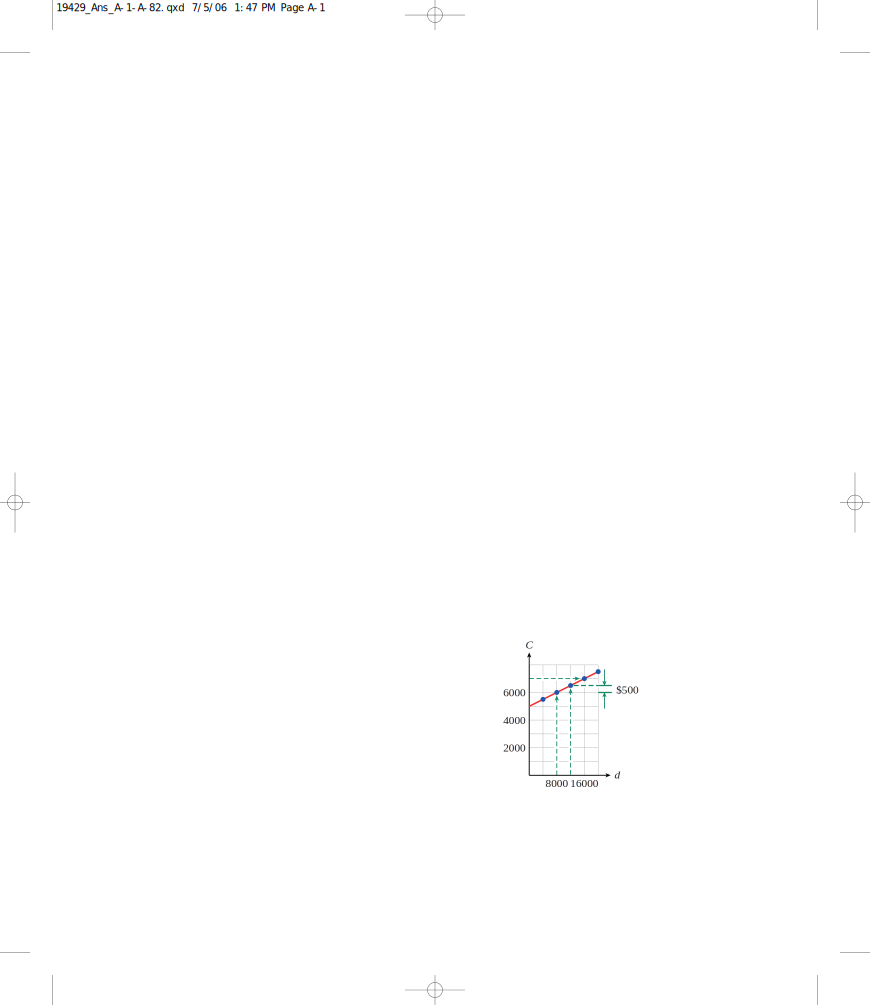
\includegraphics[width=0.5\linewidth]{images/fig-ans-1-1-7}
%
\item\hypertarget{li-165}{}\(\$500\)%
\item\hypertarget{li-166}{}More than 16,000 miles%
\end{enumerate}
%
\item[8.]\hypertarget{exercise-15}{}The boiling point of water changes with altitude. At sea level, water boils at \(212\degree\)F, and the boiling point diminishes by approximately \(0.002\degree\)F for each \(1\)-foot increase in altitude. \leavevmode%
\begin{enumerate}[label=(\alph*)]
\item\hypertarget{li-167}{}Write an equation for the boiling point, \(B\), in terms of \(a\), the altitude in feet.%
\item\hypertarget{li-168}{}Complete the table of values. \leavevmode%
\begin{table}
\centering
\begin{tabular}{AlAcAcAcAcAcAcAcA}\hrulethick
Altitude (ft)&\(-500\)&\(0\)&\(1000\)&\(2000\)&\(3000\)&\(4000\)&\(5000\)\tabularnewline\hrulethin
Boiling point (\(\degree\)F)&\(\hphantom{0000}\)&\(\hphantom{0000}\)&\(\hphantom{0000}\)&\(\hphantom{0000}\)&\(\hphantom{0000}\)&\(\hphantom{0000}\)&\(\hphantom{0000}\)\tabularnewline\hrulethin
\end{tabular}
\end{table}
%
\item\hypertarget{li-169}{}Choose scales for the axes and graph the equation.%
\item\hypertarget{li-170}{}How much does the boiling point decrease when the altitude increases from \(1000\) to \(3000\) feet? Illustrate this amount on the graph.%
\item\hypertarget{li-171}{}At what altitudes is the boiling point less than \(204\degree\)F? Illustrate on the graph.%
\end{enumerate}
%
\par\smallskip
\hypertarget{exercisegroup-1}{}\par\noindent For each table, choose appropriate scales for the axes and plot the given points.%
\begin{exercisegroup}(2)
\exercise[9.]\hypertarget{exercise-16}{}\begin{tabular}{AlAcAcAcAcA}\hrulethick
\(x\)&\(0\)&\(80\)&\(90\)&\(120\)\tabularnewline\hrulethin
\(y\)&\(6\)&\(2\)&\(1.5\)&\(1\)\tabularnewline\hrulethin
\end{tabular}
%
\par\smallskip
\noindent\textbf{Answer.}\hypertarget{answer-12}{}\quad
\includegraphics[width=0.5\linewidth]{images/fig-ans-1-1-9}
%
\exercise[10.]\hypertarget{exercise-17}{}\begin{tabular}{AlAcAcAcAcA}\hrulethick
\(x\)&\(300\)&\(500\)&\(800\)&\(1100\)\tabularnewline\hrulethin
\(y\)&\(1.2\)&\(1.3\)&\(1.5\)&\(1.9\)\tabularnewline\hrulethin
\end{tabular}
%
\exercise[11.]\hypertarget{exercise-18}{}\begin{tabular}{AlAcAcAcAcA}\hrulethick
\(x\)&\(0.01\)&\(0.03\)&\(0.06\)&\(0.07\)\tabularnewline\hrulethin
\(y\)&\(-0.2\)&\(-1\)&\(-1.1\)&\(-2\)\tabularnewline\hrulethin
\end{tabular}
%
\par\smallskip
\noindent\textbf{Answer.}\hypertarget{answer-13}{}\quad
\includegraphics[width=0.5\linewidth]{images/fig-ans-1-1-11}
%
\exercise[12.]\hypertarget{exercise-19}{}\begin{tabular}{AlAcAcAcAcA}\hrulethick
\(x\)&\(0.003\)&\(0.005\)&\(0.008\)&\(0.011\)\tabularnewline\hrulethin
\(y\)&\(6\)&\(2\)&\(1.5\)&\(1\)\tabularnewline\hrulethin
\end{tabular}
%
\end{exercisegroup}
\par\smallskip\noindent
\hypertarget{exercisegroup-2}{}\par\noindent For Problems 13-18, \leavevmode%
\begin{enumerate}[label=(\alph*)]
\item\hypertarget{li-172}{}Find the intercepts of the graph.%
\item\hypertarget{li-173}{}Graph the equation by the intercept method.%
\end{enumerate}
%
\begin{exercisegroup}(3)
\exercise[13.]\hypertarget{exercise-20}{}\(x + 2y = 8\)%
\par\smallskip
\noindent\textbf{Answer.}\hypertarget{answer-14}{}\quad
\leavevmode%
\begin{enumerate}[label=\alph*]
\item\hypertarget{li-174}{}\((8, 0), (0, 4)\)%
\item\hypertarget{li-175}{}\includegraphics[width=0.5\linewidth]{images/fig-ans-1-1-13}
%
\end{enumerate}
%
\exercise[14.]\hypertarget{exercise-21}{}\(2x - y = 6\)%
\exercise[15.]\hypertarget{exercise-22}{}\(3x - 4y =12\)%
\par\smallskip
\noindent\textbf{Answer.}\hypertarget{answer-15}{}\quad
\leavevmode%
\begin{enumerate}[label=\alph*]
\item\hypertarget{li-176}{}\((4, 0), (0, -3)\)%
\item\hypertarget{li-177}{}\includegraphics[width=0.5\linewidth]{images/fig-ans-1-1-15}
%
\end{enumerate}
%
\exercise[16.]\hypertarget{exercise-23}{}\(2x + 6y = 6\)%
\exercise[17.]\hypertarget{exercise-24}{}\(\displaystyle{\frac{x}{9}- \frac{y}{4}= 1}\)%
\par\smallskip
\noindent\textbf{Answer.}\hypertarget{answer-16}{}\quad
\leavevmode%
\begin{enumerate}[label=\alph*]
\item\hypertarget{li-178}{}\((9, 0), (0, -4)\)%
\item\hypertarget{li-179}{}\includegraphics[width=0.5\linewidth]{images/fig-ans-1-1-17}
%
\end{enumerate}
%
\exercise[18.]\hypertarget{exercise-25}{}\(\displaystyle{\frac{x}{5}+ \frac{y}{8}= 1}\)%
\end{exercisegroup}
\par\smallskip\noindent
\hypertarget{exercisegroup-3}{}\par\noindent For Problems 19-24, \leavevmode%
\begin{enumerate}[label=(\alph*)]
\item\hypertarget{li-180}{}Find the intercepts of the graph.%
\item\hypertarget{li-181}{}Use the intercepts to choose scales for the axes, and then graph the equation by the intercept method.%
\end{enumerate}
%
\begin{exercisegroup}(2)
\exercise[19.]\hypertarget{exercise-26}{}\(20x = 30y - 45,000\)%
\par\smallskip
\noindent\textbf{Answer.}\hypertarget{answer-17}{}\quad
\leavevmode%
\begin{enumerate}[label=\alph*]
\item\hypertarget{li-182}{}\((-2250, 0), (0, 1500)\)%
\item\hypertarget{li-183}{}\includegraphics[width=0.5\linewidth]{images/fig-ans-1-1-19}
%
\end{enumerate}
%
\exercise[20.]\hypertarget{exercise-27}{}\(30x = 45y + 60,000\)%
\exercise[21.]\hypertarget{exercise-28}{}\(0.4x + 1.2y = 4.8\)%
\par\smallskip
\noindent\textbf{Answer.}\hypertarget{answer-18}{}\quad
\leavevmode%
\begin{enumerate}[label=\alph*]
\item\hypertarget{li-184}{}\((12, 0), (0, 4)\)%
\item\hypertarget{li-185}{}\includegraphics[width=0.5\linewidth]{images/fig-ans-1-1-21}
%
\end{enumerate}
%
\exercise[22.]\hypertarget{exercise-29}{}\(3.2x - 0.8y = 12.8\)%
\exercise[23.]\hypertarget{exercise-30}{}\(\displaystyle{\frac{2x}{3}+ \frac{3y}{11}= 1}\)%
\par\smallskip
\noindent\textbf{Answer.}\hypertarget{answer-19}{}\quad
\leavevmode%
\begin{enumerate}[label=\alph*]
\item\hypertarget{li-186}{}\(\left(\dfrac{3}{2} , 0\right), \left(0, \dfrac{11}{3} \right)\)%
\item\hypertarget{li-187}{}\includegraphics[width=0.5\linewidth]{images/fig-ans-1-1-23}
%
\end{enumerate}
%
\exercise[24.]\hypertarget{exercise-31}{}\(\displaystyle{\frac{8x}{7}- \frac{2y}{7}= 1}\)%
\end{exercisegroup}
\par\smallskip\noindent
\item[25.]\hypertarget{exercise-32}{}The owner of a gas station has \(\$19,200\) to spend on unleaded gas this month. Regular unleaded costs him \(\$2.40\) per gallon, and premium unleaded costs \(\$3.20\) per gallon.%
\leavevmode%
\begin{enumerate}[label=\alph*]
\item\hypertarget{li-188}{}How much do \(x\) gallons of regular cost? How much do \(y\) gallons of premium cost?%
\item\hypertarget{li-189}{}Write an equation in general form that relates the amount of regular unleaded gasoline, \(\), the owner can buy and the amount of premium unleaded, \(y\).%
\item\hypertarget{li-190}{}Find the intercepts and sketch the graph.%
\item\hypertarget{li-191}{}What do the intercepts tell us about the amount of gasoline the owner can purchase?%
\end{enumerate}
\par\smallskip
\par\smallskip
\noindent\textbf{Answer.}\hypertarget{answer-20}{}\quad
\leavevmode%
\begin{enumerate}[label=\alph*]
\item\hypertarget{li-192}{}\(\$2.40x, \$3.20y\)%
\item\hypertarget{li-193}{}\(2.40x + 3.20y = 19,200\)%
\item\hypertarget{li-194}{}\includegraphics[width=0.5\linewidth]{images/fig-ans-1-1-25}
%
\item\hypertarget{li-195}{}The \(y\)-intercept, \(6000\) gallons, is the amount of premium that the gas station owner can buy if he buys no regular. The \(x\)-intercept, \(8000\) gallons, is the amount of regular he can buy if he buys no premium.%
\end{enumerate}
%
\item[26.]\hypertarget{exercise-33}{}Five pounds of body fat is equivalent to \(16,000\) calories. Carol can burn \(600\) calories per hour bicycling and \(400\) calories per hour swimming.%
\leavevmode%
\begin{enumerate}[label=\alph*]
\item\hypertarget{li-196}{}How many calories will Carol burn in \(\) hours of cycling? How many calories will she burn in \(y\) hours of swimming?%
\item\hypertarget{li-197}{}Write an equation in general form that relates the number of hours, \(x\), of cycling and the number of hours, \(y\), of swimming Carol needs to perform in order to lose \(5\) pounds.%
\item\hypertarget{li-198}{}Find the intercepts and sketch the graph.%
\item\hypertarget{li-199}{}What do the intercepts tell us about Carol's exercise program?%
\end{enumerate}
\par\smallskip
\item[27.]\hypertarget{exercise-34}{}Delbert must increase his daily potassium intake by \(1800\) mg. He decides to eat a combination of figs and bananas, which are both low in sodium. There are \(9\) mg potassium per gram of fig, and \(4\) mg potassium per gram of banana.%
\leavevmode%
\begin{enumerate}[label=\alph*]
\item\hypertarget{li-200}{}How much potassium is in \(x\) grams of fig? How much potassium is in \(y\) grams of banana?%
\item\hypertarget{li-201}{}Write an equation in general form that relates the number of grams, \(x\), of fig and the number of grams, \(y\), of banana Delbert needs to get \(1800\) mg of potassium.%
\item\hypertarget{li-202}{}Find the intercepts and sketch the graph.%
\item\hypertarget{li-203}{}What do the intercepts tell us about Delbert's diet?%
\end{enumerate}
\par\smallskip
\par\smallskip
\noindent\textbf{Answer.}\hypertarget{answer-21}{}\quad
\leavevmode%
\begin{enumerate}[label=\alph*]
\item\hypertarget{li-204}{}\(9x\) mg, \(4y\) mg%
\item\hypertarget{li-205}{}\(9x + 4y = 1800\)%
\item\hypertarget{li-206}{}\includegraphics[width=0.35\linewidth]{images/fig-ans-1-1-27}
%
\item\hypertarget{li-207}{}The \(x\)-intercept, \(200\) grams, tells how much fig Delbert should eat if he has no bananas, and the \(y\)-intercept, \(450\) grams, tells how much banana he should eat if he has no figs.%
\end{enumerate}
%
\item[28.]\hypertarget{exercise-35}{}Leslie plans to invest some money in two CD accounts. The first account pays \(3.6\%\) interest per year, and the second account pays \(2.8\%\) interest per year. Leslie would like to earn \(\$500\) per year on her investment.%
\leavevmode%
\begin{enumerate}[label=\alph*]
\item\hypertarget{li-208}{}If Leslie invests \(x\) dollars in the first account, how much interest will she earn? How much interest will she earn if she invests \(y\) dollars in the second account?%
\item\hypertarget{li-209}{}Write an equation in general form that relates \(x\) and \(y\) if Leslie earns \(\$500\) interest.%
\item\hypertarget{li-210}{}Find the intercepts and sketch the graph.%
\item\hypertarget{li-211}{}What do the intercepts tell us about Leslie's investments?%
\end{enumerate}
\par\smallskip
\item[29.]\hypertarget{exercise-36}{}Find the intercepts of the graph for each equation.%
\leavevmode%
\begin{multicols}{2}
\begin{enumerate}[label=\alph*]
\item\hypertarget{li-212}{}\(\displaystyle{\frac{x}{3}+\frac{y}{5}=1} \)%
\item\hypertarget{li-213}{}\(\displaystyle{2x - 4y = 1} \)%
\item\hypertarget{li-214}{}\(\displaystyle{\frac{2x}{5}-\frac{2y}{3}=1} \)%
\item\hypertarget{li-215}{}\(\displaystyle{\frac{x}{p}+\frac{y}{q}=1} \)%
\item\hypertarget{li-216}{}Why is the equation \(\displaystyle{\frac{x}{a}+\frac{y}{b}=1} \) called the \terminology{intercept form} for a line?%
\end{enumerate}
\end{multicols}
\par\smallskip
\par\smallskip
\noindent\textbf{Answer.}\hypertarget{answer-22}{}\quad
\leavevmode%
\begin{multicols}{2}
\begin{enumerate}[label=\alph*]
\item\hypertarget{li-217}{}\((3,0), (0,5) \)%
\item\hypertarget{li-218}{}\(\left(\dfrac{1}{2},0\right), \left(0,\dfrac{-1}{4}\right) \)%
\item\hypertarget{li-219}{}\(\left(\dfrac{5}{2},0\right), \left(0,\dfrac{-3}{2}\right) \)%
\item\hypertarget{li-220}{}\((p,0), (0,q) \)%
\item\hypertarget{li-221}{}The value of \(a\) is the \(x\)-intercept, and the value of \(b\) is the \(y\)-intercept.%
\end{enumerate}
\end{multicols}
%
\item[30.]\hypertarget{exercise-37}{}Write an equation in intercept form (see Problem 29) for the line with the given intercepts. Then write the equation in general form.%
\leavevmode%
\begin{multicols}{2}
\begin{enumerate}[label=\alph*]
\item\hypertarget{li-222}{}\((6, 0), (0, 2) \)%
\item\hypertarget{li-223}{}\((-3, 0), (0, 8) \)%
\item\hypertarget{li-224}{}\(\left(\dfrac{3}{4}, 0\right), \left(0, \dfrac{-1}{4}\right) \)%
\item\hypertarget{li-225}{}\((v, 0), (0, -w) \)%
\item\hypertarget{li-226}{}\(\left(\dfrac{1}{H}, 0\right), \left(0, \dfrac{1}{T}\right) \)%
\end{enumerate}
\end{multicols}
\par\smallskip
\item[31.]\hypertarget{exercise-38}{}\leavevmode%
\begin{enumerate}[label=\alph*]
\item\hypertarget{li-227}{}Find the \(y\)-intercept of the line \(y = mx + b\).%
\item\hypertarget{li-228}{}Find the \(x\)-intercept of the line \(y = mx + b\).%
\end{enumerate}
%
\par\smallskip
\par\smallskip
\noindent\textbf{Answer.}\hypertarget{answer-23}{}\quad
\leavevmode%
\begin{enumerate}[label=\alph*]
\item\hypertarget{li-229}{}\((0, b)\)%
\item\hypertarget{li-230}{}\(\left(\dfrac{-b}{m},0\right)\), if \(m\ne 0\)%
\end{enumerate}
%
\item[32.]\hypertarget{exercise-39}{}\leavevmode%
\begin{enumerate}[label=\alph*]
\item\hypertarget{li-231}{}Find the \(y\)-intercept of the line \(Ax + By = C\).%
\item\hypertarget{li-232}{}Find the \(x\)-intercept of the line \(Ax + By = C\).%
\end{enumerate}
%
\par\smallskip
\end{exerciselist}
\hypertarget{exercisegroup-4}{}\par\noindent Write an equation in general form for each line.%
\begin{exercisegroup}(2)
\exercise[33.]\hypertarget{exercise-40}{}\includegraphics[width=0.8\linewidth]{images/fig-ex-1-1-33}
%
\par\smallskip
\noindent\textbf{Answer.}\hypertarget{answer-24}{}\quad
\(-2x + 3y = 2400\)%
\exercise[34.]\hypertarget{exercise-41}{}\includegraphics[width=0.8\linewidth]{images/fig-ex-1-1-34}
%
\exercise[35.]\hypertarget{exercise-42}{}\includegraphics[width=0.8\linewidth]{images/fig-ex-1-1-35}
%
\par\smallskip
\noindent\textbf{Answer.}\hypertarget{answer-25}{}\quad
\(3x + 400y = 240\)%
\exercise[36.]\hypertarget{exercise-43}{}\includegraphics[width=0.8\linewidth]{images/fig-ex-1-1-36}
%
\end{exercisegroup}
\par\smallskip\noindent
\hypertarget{exercisegroup-5}{}\par\noindent For Problems 37–44, \leavevmode%
\begin{enumerate}[label=\alph*]
\item\hypertarget{li-233}{}Solve each equation for \(y\) in terms of \(x\). (See the Algebra Skills Refresher {$\langle\langle$Unresolved xref, reference "appendix-Linear-Equations-and-Inequalities"; check spelling or use "provisional" attribute$\rangle\rangle$} to review this skill.)%
\item\hypertarget{li-234}{}Graph the equation on your calculator in the specified window. (See {$\langle\langle$Unresolved xref, reference "appendix-b"; check spelling or use "provisional" attribute$\rangle\rangle$} for help with the graphing calculator.)%
\item\hypertarget{li-235}{}Make a pencil and paper sketch of the graph. Label the scales on your axes, and the coordinates of the intercepts.%
\end{enumerate}
%
\begin{exercisegroup}(2)
\exercise[37.]\hypertarget{exercise-44}{}\(2+y=6\)%
\begin{align*}
\small{\text{Xmin}} \amp = -10 \amp\amp \small{\text{Ymin}} = -10
\\
\small{\text{Xmax}} \amp = 10 \amp\amp \small{\text{Ymax}} = 10
\\
\small{\text{Xscl}} \amp = 1 \amp\amp \small{\text{Yscl}} = 1
\end{align*}
%
\par\smallskip
\noindent\textbf{Answer.}\hypertarget{answer-26}{}\quad
\leavevmode%
\begin{description}
\item[{a.}]\hypertarget{li-236}{}\(y = 6 - 2x\)%
\item[{c.}]\hypertarget{li-237}{}\includegraphics[width=0.5\linewidth]{images/fig-ans-1-1-37}
%
\end{description}
%
\exercise[38.]\hypertarget{exercise-45}{}\(8 - y + 3x = 0\)%
\begin{align*}
\small{\text{Xmin}} \amp = -10 \amp\amp \small{\text{Ymin}} = -10
\\
\small{\text{Xmax}} \amp = 10 \amp\amp \small{\text{Ymax}} = 10
\\
\small{\text{Xscl}} \amp = 1 \amp\amp \small{\text{Yscl}} = 1
\end{align*}
%
\exercise[39.]\hypertarget{exercise-46}{}\(3x - 4y = 1200\)%
\begin{align*}
\small{\text{Xmin}} \amp = -1000 \amp\amp \small{\text{Ymin}} = -1000
\\
\small{\text{Xmax}} \amp = 1000 \amp\amp \small{\text{Ymax}} = 1000
\\
\small{\text{Xscl}} \amp = 100 \amp\amp \small{\text{Yscl}} = 100
\end{align*}
%
\par\smallskip
\noindent\textbf{Answer.}\hypertarget{answer-27}{}\quad
\leavevmode%
\begin{description}
\item[{a.}]\hypertarget{li-238}{}\(y = \dfrac{3}{4}x-300\)%
\item[{c.}]\hypertarget{li-239}{}\includegraphics[width=0.5\linewidth]{images/fig-ans-1-1-39}
%
\end{description}
%
\exercise[40.]\hypertarget{exercise-47}{}\(x + 2y = 500\)%
\begin{align*}
\small{\text{Xmin}} \amp = -1000 \amp\amp \small{\text{Ymin}} = -1000
\\
\small{\text{Xmax}} \amp = 1000 \amp\amp \small{\text{Ymax}} = 1000
\\
\small{\text{Xscl}} \amp = 100 \amp\amp \small{\text{Yscl}} = 100
\end{align*}
%
\exercise[41.]\hypertarget{exercise-48}{}\(0.2x + 5y = 0.1\)%
\begin{align*}
\small{\text{Xmin}} \amp = -1 \amp\amp \small{\text{Ymin}} = -0.1
\\
\small{\text{Xmax}} \amp = 1 \amp\amp \small{\text{Ymax}} = 0.1
\\
\small{\text{Xscl}} \amp = 0.1 \amp\amp \small{\text{Yscl}} = 0.01
\end{align*}
%
\par\smallskip
\noindent\textbf{Answer.}\hypertarget{answer-28}{}\quad
\leavevmode%
\begin{description}
\item[{a.}]\hypertarget{li-240}{}\(y = 0.02 - 0.04x\)%
\item[{c.}]\hypertarget{li-241}{}\includegraphics[width=0.5\linewidth]{images/fig-ans-1-1-41}
%
\end{description}
%
\exercise[42.]\hypertarget{exercise-49}{}\(1.2x - 4.2y = 3.6\)%
\begin{align*}
\small{\text{Xmin}} \amp = -1 \amp\amp \small{\text{Ymin}} = -1
\\
\small{\text{Xmax}} \amp = 4 \amp\amp \small{\text{Ymax}} = 1
\\
\small{\text{Xscl}} \amp = 0.2 \amp\amp \small{\text{Yscl}} = 0.1
\end{align*}
%
\exercise[43.]\hypertarget{exercise-50}{}\(70x + 3y = y + 420\)%
\begin{align*}
\small{\text{Xmin}} \amp = 0 \amp\amp \small{\text{Ymin}} = 0
\\
\small{\text{Xmax}} \amp = 10 \amp\amp \small{\text{Ymax}} = 250
\\
\small{\text{Xscl}} \amp = 1 \amp\amp \small{\text{Yscl}} = 25
\end{align*}
%
\par\smallskip
\noindent\textbf{Answer.}\hypertarget{answer-29}{}\quad
\leavevmode%
\begin{description}
\item[{a.}]\hypertarget{li-242}{}\(y = 210 - 35x\)%
\item[{c.}]\hypertarget{li-243}{}\includegraphics[width=0.5\linewidth]{images/fig-ans-1-1-43}
%
\end{description}
%
\exercise[44.]\hypertarget{exercise-51}{}\(40y - 5x = 780 - 20y\)%
\begin{align*}
\small{\text{Xmin}} \amp = -200 \amp\amp \small{\text{Ymin}} = 0
\\
\small{\text{Xmax}} \amp = 0 \amp\amp \small{\text{Ymax}} = 20
\\
\small{\text{Xscl}} \amp = 20 \amp\amp \small{\text{Yscl}} = 2
\end{align*}
%
\end{exercisegroup}
\par\smallskip\noindent
\hypertarget{exercisegroup-6}{}\par\noindent For Problems 45–52, \leavevmode%
\begin{enumerate}[label=\alph*]
\item\hypertarget{li-244}{}Find the \(\text{}\)- and \(y\)-intercepts.%
\item\hypertarget{li-245}{}Solve the equation for \(y\).%
\item\hypertarget{li-246}{}Choose a graphing window in which both intercepts are visible, and graph the equation on your calculator.%
\end{enumerate}
%
\begin{exercisegroup}(2)
\exercise[45.]\hypertarget{exercise-52}{}\(x + 4y = 100\)%
\par\smallskip
\noindent\textbf{Answer.}\hypertarget{answer-30}{}\quad
\leavevmode%
\begin{enumerate}[label=\alph*]
\item\hypertarget{li-247}{}\((100, 0), (0, 25)\)%
\item\hypertarget{li-248}{}\(y = 25 - \dfrac{1}{4}x\)%
\item\hypertarget{li-249}{}\includegraphics[width=0.5\linewidth]{images/fig-ans-1-1-45.jpg}
%
\end{enumerate}
%
\exercise[46.]\hypertarget{exercise-53}{}\(2x - 3y = -72\)%
\exercise[47.]\hypertarget{exercise-54}{}\(25x - 20y = 1\)%
\par\smallskip
\noindent\textbf{Answer.}\hypertarget{answer-31}{}\quad
\leavevmode%
\begin{enumerate}[label=\alph*]
\item\hypertarget{li-250}{}\((0.04, 0), (0, -0.05)\)%
\item\hypertarget{li-251}{}\(y = 1.25x - 0.05\)%
\item\hypertarget{li-252}{}\includegraphics[width=0.5\linewidth]{images/fig-ans-1-1-47.jpg}
%
\end{enumerate}
%
\exercise[48.]\hypertarget{exercise-55}{}\(4x + 75y = 60,000\)%
\exercise[49.]\hypertarget{exercise-56}{}\(\dfrac{y}{12} - \dfrac{x}{60}= 1\)%
\par\smallskip
\noindent\textbf{Answer.}\hypertarget{answer-32}{}\quad
\leavevmode%
\begin{enumerate}[label=\alph*]
\item\hypertarget{li-253}{}\((-60, 0), (0, 12)\)%
\item\hypertarget{li-254}{}\(y = 12 + \dfrac{1}{5}x\)%
\item\hypertarget{li-255}{}\includegraphics[width=0.5\linewidth]{images/fig-ans-1-1-49.jpg}
%
\end{enumerate}
%
\exercise[50.]\hypertarget{exercise-57}{}\(\dfrac{x}{80} + \dfrac{y}{400}= 1\)%
\exercise[51.]\hypertarget{exercise-58}{}\(-2x = 3y + 84\)%
\par\smallskip
\noindent\textbf{Answer.}\hypertarget{answer-33}{}\quad
\leavevmode%
\begin{enumerate}[label=\alph*]
\item\hypertarget{li-256}{}\((-42, 0), (0, -28)\)%
\item\hypertarget{li-257}{}\(y = \dfrac{-2}{3}x-28\)%
\item\hypertarget{li-258}{}\includegraphics[width=0.5\linewidth]{images/fig-ans-1-1-51.jpg}
%
\end{enumerate}
%
\exercise[52.]\hypertarget{exercise-59}{}\(7x = 91 - 13y\)%
\end{exercisegroup}
\par\smallskip\noindent
\typeout{************************************************}
\typeout{Section 1.2 Functions}
\typeout{************************************************}
\section[{Functions}]{Functions}\label{functions}
\typeout{************************************************}
\typeout{Subsection 1.2.1 Definition of Function}
\typeout{************************************************}
\subsection[{Definition of Function}]{Definition of Function}\label{subsection-7}
We often want to predict values of one variable from the values of a related variable. For example, when a physician prescribes a drug in a certain dosage, she needs to know how long the dose will remain in the bloodstream. A sales manager needs to know how the price of his product will affect its sales. A \terminology{function} is a special type of relationship between variables that allows us to make such predictions.%
\par
Suppose it costs \textdollar{}800 for flying lessons, plus \textdollar{}30 per hour to rent a plane. If we let \(C\) represent the total cost for \(t\) hours of flying lessons, then%
\begin{equation*}
C=800+305t ~~~~ (t\ge 0)
\end{equation*}
Thus, for example%
\begin{table}
\centering
\begin{tabular}{rll}
when&\(t=\alert{0}\),&\(C=800+30(\alert{0})=800\)\tabularnewline[0pt]
when&\(t=\alert{4}\),&\(C=800+30(\alert{4})=920\)\tabularnewline[0pt]
when&\(t=\alert{10}\),&\(C=800+30(\alert{10})=1100\)
\end{tabular}
\end{table}
The variable \(t\) is called the \terminology{input} or \terminology{independent} variable, and \(C\) is the \terminology{output} or \terminology{dependent} variable, because its values are determined by the value of \(t\). We can display the relationship between two variables by a table or by ordered pairs. The input variable is the first component of the ordered pair, and the output variable is the second component.%
\begin{table}
\centering
\begin{tabular}{AcAcAcA}\hrulethick
\(t\)&\(C\)&\((t,C)\)\tabularnewline\hrulethin
\(0\)&\(800\)&\((0, 800)\)\tabularnewline\hrulethin
\(4\)&\(920\)&\((4, 920)\)\tabularnewline\hrulethin
\(10\)&\(1100\)&\((10,1100)\)\tabularnewline\hrulethin
\end{tabular}
\end{table}
For this relationship, we can find the value \(C\) of associated with any given value of \(t\). All we have to do is substitute the value of \(t\) into the equation and solve for \(C\). The result has no ambiguity: Only one value for \(C\) corresponds to each value of \(t\). This type of relationship between variables is called a \terminology{function}. In general, we make the following definition.%
\begin{assemblage}{Definition of Function}\label{assemblage-6}
A \terminology{function} is a relationship between two variables for which a unique value of the \terminology{output} variable can be determined from a value of the \terminology{input} variable.%
\end{assemblage}
What distinguishes functions from other variable relationships? The definition of a function calls for a \emph{unique value}—that is, \emph{exactly one value} of the output variable corresponding to each value of the input variable. This property makes functions useful in applications because they can often be used to make predictions.%
\begin{example}[]\label{example-functions}
\leavevmode%
\begin{enumerate}[label=\alph*]
\item\hypertarget{li-259}{}The distance, \(d\), traveled by a car in 2 hours is a function of its speed, \(r\). If we know the speed of the car, we can determine the distance it travels by the formula \(d = r \cdot 2\).%
\item\hypertarget{li-260}{}The cost of a fill-up with unleaded gasoline is a function of the number of gallons purchased. The gas pump represents the function by displaying the corresponding values of the input variable (number of gallons) and the output variable (cost).%
\item\hypertarget{li-261}{}Score on the Scholastic Aptitude Test (SAT) is not a function of score on an IQ test, because two people with the same score on an IQ test may score differently on the SAT; that is, a person’s score on the SAT is not uniquely determined by his or her score on an IQ test.%
\end{enumerate}
%
\end{example}
\begin{exercise}\label{exercise-functions}
\leavevmode%
\begin{enumerate}[label=\alph*]
\item\hypertarget{li-262}{}As part of a project to improve the success rate of freshmen, the counseling department studied the grades earned by a group of students in English and algebra. Do you think that a student’s grade in algebra is a function of his or her grade in English? Explain why or why not.%
\item\hypertarget{li-263}{}Phatburger features a soda bar, where you can serve your own soft drinks in any size. Do you think that the number of calories in a serving of Zap Kola is a function of the number of fluid ounces? Explain why or why not.%
\end{enumerate}
%
\end{exercise}
\typeout{************************************************}
\typeout{Subsection 1.2.2 Functions Defined by Tables}
\typeout{************************************************}
\subsection[{Functions Defined by Tables}]{Functions Defined by Tables}\label{subsection-8}
When we use a table to describe a function, the first variable in the table (the left column of a vertical table or the top row of a horizontal table) is the input variable, and the second variable is the output. We say that the output variable is a function of the input.%
\begin{example}[]\label{example-table-functions}
\leavevmode%
\begin{enumerate}[label=\alph*]
\item\hypertarget{li-266}{}\hyperref[table-auto-sales]{Table~\ref{table-auto-sales}} shows data on sales compiled over several years by the accounting office for Eau Claire Auto Parts, a division of Major Motors. In this example, the year is the input variable, and total sales is the output. We say that total sales, \(S\), is a function of \(t\).%
\begin{table}
\centering
\begin{tabular}{AcAcA}\hrulethick
Year \((t)\)&Total sales \((S)\)\tabularnewline\hrulethin
2000&\textdollar{}612,000\tabularnewline\hrulethin
2001&\textdollar{}663,000\tabularnewline\hrulethin
2002&\textdollar{}692,000\tabularnewline\hrulethin
2003&\textdollar{}749,000\tabularnewline\hrulethin
2004&\textdollar{}904,000\tabularnewline\hrulethin
\end{tabular}
\caption{\label{table-auto-sales}}
\end{table}
\item\hypertarget{li-267}{}\hyperref[table-postage]{Table~\ref{table-postage}} gives the cost of sending printed material by first-class mail in 2016.%
\begin{table}
\centering
\begin{tabular}{AcAcA}\hrulethick
Weight in ounces \((w)\)&Postage \((P)\)\tabularnewline\hrulethin
\(0 \lt w \le 1 \)&\textdollar{}0.47\tabularnewline\hrulethin
\(1 \lt w \le 2 \)&\textdollar{}0.68\tabularnewline\hrulethin
\(2 \lt w \le 3 \)&\textdollar{}0.89\tabularnewline\hrulethin
\(3 \lt w \le 4 \)&\textdollar{}1.10\tabularnewline\hrulethin
\(4 \lt w \le 5 \)&\textdollar{}1.31\tabularnewline\hrulethin
\(5 \lt w \le 6 \)&\textdollar{}1.52\tabularnewline\hrulethin
\(6 \lt w \le 7 \)&\textdollar{}1.73\tabularnewline\hrulethin
\end{tabular}
\caption{\label{table-postage}}
\end{table}
If we know the weight of the article being shipped, we can determine the required postage from \hyperref[table-postage]{Table~\ref{table-postage}}. For instance, a catalog weighing 4.5 ounces would require \textdollar{}1.31 in postage. In this example, \(w\) is the input variable and \(p\) is the output variable. We say that \(p\) \emph{is a function of} \(w\).%
\item\hypertarget{li-268}{}\hyperref[table-cholesterol]{Table~\ref{table-cholesterol}} records the age and cholesterol count for 20 patients tested in a hospital survey.%
\begin{table}
\centering
\begin{tabular}{AcAcAcAcAcA}\hrulethick
Age&Cholesterol count&&Age&Cholesterol count\tabularnewline\hrulethin
53&217&&\(\alert{51}\)&\(\alert{209}\)\tabularnewline\hrulethin
48&232&&53&241\tabularnewline\hrulethin
55&198&&49&186\tabularnewline\hrulethin
56&238&&\(\alert{51}\)&\(\alert{216}\)\tabularnewline\hrulethin
\(\alert{51}\)&\(\alert{227}\)&&57&208\tabularnewline\hrulethin
52&264&&52&248\tabularnewline\hrulethin
53&195&&50&214\tabularnewline\hrulethin
47&203&&56&271\tabularnewline\hrulethin
48&212&&53&193\tabularnewline\hrulethin
50&234&&48&172\tabularnewline\hrulethin
\end{tabular}
\caption{\label{table-cholesterol}}
\end{table}
According to these data, cholesterol count is \emph{not} a function of age, because several patients who are the same age have different cholesterol levels. For example, three different patients are 51 years old but have cholesterol counts of 227, 209, and 216, respectively. Thus, we cannot determine a \emph{unique} value of the output variable (cholesterol count) from the value of the input variable (age). Other factors besides age must influence a person’s cholesterol count.%
\end{enumerate}
\end{example}
\begin{exercise}\label{exercise-61}
Decide whether each table describes \(y\) as a function of \(x\). Explain your choice. \leavevmode%
\begin{enumerate}[label=\alph*]
\item\hypertarget{li-269}{}\begin{tabular}{AcAcAcAcAcAcAcAcAcA}\hrulethick
\(x\)&\(3.5\)&\(2.0\)&\(2.5\)&\(3.5\)&\(2.5\)&\(4.0\)&\(2.5\)&\(3.0\)\tabularnewline\hrulethin
\(y\)&\(2.5\)&\(3.0\)&\(2.5\)&\(4.0\)&\(3.5\)&\(4.0\)&\(2.0\)&\(2.5\)\tabularnewline\hrulethin
\end{tabular}
%
\item\hypertarget{li-270}{}\begin{tabular}{AcAcAcAcAcAcAcAcA}\hrulethick
\(x\)&\(-3\)&\(-2\)&\(-1\)&\(0\)&\(1\)&\(2\)&\(3\)\tabularnewline\hrulethin
\(y\)&\(17\)&\(3\)&\(0\)&\(-1\)&\(0\)&\(3\)&\(17\)\tabularnewline\hrulethin
\end{tabular}
%
\end{enumerate}
\end{exercise}
\typeout{************************************************}
\typeout{Subsection 1.2.3 Functions Defined by Graphs}
\typeout{************************************************}
\subsection[{Functions Defined by Graphs}]{Functions Defined by Graphs}\label{subsection-9}
A graph may also be used to define one variable as a function of another. The input variable is displayed on the horizontal axis, and the output variable on the vertical axis.%
\begin{example}[]\label{example-sun-hours}
\hyperref[fig-sun-hours]{Figure~\ref{fig-sun-hours}}  shows the number of hours, \(H\), that the sun is above the horizon in Peoria, Illinois, on day \(t\), where January 1 corresponds to \(t = 0\).%
% group protects changes to lengths, releases boxes (?)
{% begin: group for a single side-by-side
% set panel max height to practical minimum, created in preamble
\setlength{\panelmax}{0pt}
\newsavebox{\panelboxAparagraphs}
\savebox{\panelboxAparagraphs}{%
\raisebox{\depth}{\parbox{0.5\textwidth}{\leavevmode%
\begin{enumerate}[label=\alph*]
\item\hypertarget{li-273}{}Which variable is the input, and which is the output?%
\item\hypertarget{li-274}{}Approximately how many hours of sunlight are there in Peoria on day 150?%
\item\hypertarget{li-275}{}On which days are there 12 hours of sunlight?%
\item\hypertarget{li-276}{}What are the maximum and minimum values of \(H\), and when do these valuesoccur?%
\end{enumerate}
%
}}}
\newlength{\phAparagraphs}\setlength{\phAparagraphs}{\ht\panelboxAparagraphs+\dp\panelboxAparagraphs}
\settototalheight{\phAparagraphs}{\usebox{\panelboxAparagraphs}}
\setlength{\panelmax}{\maxof{\panelmax}{\phAparagraphs}}
\newsavebox{\panelboxAVimage}
\savebox{\panelboxAVimage}{%
\includegraphics[width=0.5\linewidth]{images/fig-sun-hours}
}
\newlength{\phAVimage}\setlength{\phAVimage}{\ht\panelboxAVimage+\dp\panelboxAVimage}
\settototalheight{\phAVimage}{\usebox{\panelboxAVimage}}
\setlength{\panelmax}{\maxof{\panelmax}{\phAVimage}}
\leavevmode%
% begin: side-by-side as figure/tabular
% \tabcolsep change local to group
\setlength{\tabcolsep}{0\textwidth}
% @{} suppress \tabcolsep at extremes, so margins behave as intended
\begin{figure}
\begin{tabular}{@{}*{2}{c}@{}}
\begin{minipage}[c][\panelmax][t]{0.5\textwidth}\usebox{\panelboxAparagraphs}\end{minipage}&
\begin{minipage}[c][\panelmax][t]{0.5\textwidth}\usebox{\panelboxAVimage}\end{minipage}\tabularnewline
&
\parbox[t]{0.5\textwidth}{\captionof{figure}{\label{fig-sun-hours}}
}\end{tabular}
\end{figure}
% end: side-by-side as tabular/figure
}% end: group for a single side-by-side
\par\medskip\noindent%
\textbf{Solution.}\quad \leavevmode%
\begin{enumerate}[label=\alph*]
\item\hypertarget{li-277}{}The input variable, \(t\), appears on the horizontal axis. The number of daylight hours, \(H\), is a function of the date. The output variable appears on the vertical axis.%
\item\hypertarget{li-278}{}The point on the curve where \(t = 150\) has \(H \approx 14.1\), so Peoria gets about 14.1 hours of daylight when \(t = 150\), which is at the end of May.%
\item\hypertarget{li-279}{}\(H = 12\) at the two points where \(t \approx 85\) (in late March) and \(t \approx 270\) (late September).%
\item\hypertarget{li-280}{}The maximum value of 14.4 hours occurs on the longest day of the year, when \(t \approx 170\), about three weeks into June. The minimum of 9.6 hours occurs on the shortest day, when \(t \approx 355\), about three weeks into December.%
\end{enumerate}
\end{example}
\begin{exercise}\label{exercise-LA-marathon}
\hyperref[fig-LA-marathon]{Figure~\ref{fig-LA-marathon}}  shows the elevation in feet, \(a\), of the Los Angeles Marathon course at a distance \(d\) miles into the race. (Source: \emph{Los Angeles Times}, March 3, 2005) \begin{figure}
\centering
\includegraphics[width=1\linewidth]{images/fig-LA-marathon}
\caption{\label{fig-LA-marathon}}
\end{figure}
\leavevmode%
\begin{enumerate}[label=\alph*]
\item\hypertarget{li-281}{}Which variable is the input, and which is the output?%
\item\hypertarget{li-282}{}What is the elevation at mile 20?%
\item\hypertarget{li-283}{}At what distances is the elevation 150 feet?%
\item\hypertarget{li-284}{}What are the maximum and minimum values of \(a\), and when do these values occur?%
\item\hypertarget{li-285}{}The runners pass by the Los Angeles Coliseum at about 4.2 miles into the race. What is the elevation there?%
\end{enumerate}
\end{exercise}
\typeout{************************************************}
\typeout{Subsection 1.2.4 Functions Defined by Equations}
\typeout{************************************************}
\subsection[{Functions Defined by Equations}]{Functions Defined by Equations}\label{subsection-10}
\hyperref[example-falling-book]{Example~\ref{example-falling-book}} illustrates a function defined by an equation.%
\begin{example}[]\label{example-falling-book}
As of 2016,  One World Trade Center in New York City is the nation’s tallest building, at 1776 feet. If an algebra book is dropped from the top of the Sears Tower, its height above the ground after \(t\) seconds is given by the equation%
\begin{equation*}
h = 1776 - 16t^2
\end{equation*}
Thus, after \(\alert{1}\) second the book’s height is%
\begin{equation*}
h = 1776 - 16(\alert{1})^2 = 1760 \text{ feet}
\end{equation*}
After \(\alert{2}\) seconds its height is%
\begin{equation*}
h = 1776 - 16(\alert{2})^2 = 1712 \text{ feet}
\end{equation*}
For this function, \(t\) is the input variable and \(h\) is the output variable. For any value of \(t\), a unique value of \(h\) can be determined from the equation for \(h\). We say that \(h\) \emph{is a function of} \(t\).%
\end{example}
\begin{exercise}\label{exercise-63}
Write an equation that gives the volume, \(V\), of a sphere as a function of its radius, \(r\).\end{exercise}
\begin{remark}[Making a Table of Values with a Calculator]\label{remark-3}
We can use a graphing calculator to make a table of values for a function defined by an equation. For the function in \hyperref[example-falling-book]{Example~\ref{example-falling-book}},%
\begin{equation*}
h = 1776 - 16t^2
\end{equation*}
we begin by entering the equation: Press the \lstinline?Y=? key, clear out any other equations, and define \(Y_1 = 1776 - 16X^2.\)%
\par
Next, we choose the \(x\)-values for the table. Press \lstinline?2nd?\lstinline?WINDOW? to access the TblSet (Table Setup) menu and set it to look like \hyperref[fig-TblSetup]{Figure~\ref{fig-TblSetup}}. This setting will give us an initial x-value of 0 \((TblStart = 0)\) and an increment of one unit in the \(x\)-values, \((\Delta Tbl = 1)\). It also fills in values of both variables automatically. Now press \lstinline?2nd? \lstinline?GRAPH? to see the table of values, as shown in \hyperref[fig-GC-table]{Figure~\ref{fig-GC-table}}. From this table, we can check the heights we found in \hyperref[example-falling-book]{Example~\ref{example-falling-book}}.%
\par
Now try making a table of values with \(TblStart = 0\) and \(\Delta Tbl = 0.5\). Use the   \lstinline?↑? and \lstinline?↓? arrow keys to scroll up and down the table.%
% group protects changes to lengths, releases boxes (?)
{% begin: group for a single side-by-side
% set panel max height to practical minimum, created in preamble
\setlength{\panelmax}{0pt}
\newsavebox{\panelboxAXimage}
\savebox{\panelboxAXimage}{%
\includegraphics[width=0.5\linewidth]{images/fig-TblSetup}
}
\newlength{\phAXimage}\setlength{\phAXimage}{\ht\panelboxAXimage+\dp\panelboxAXimage}
\settototalheight{\phAXimage}{\usebox{\panelboxAXimage}}
\setlength{\panelmax}{\maxof{\panelmax}{\phAXimage}}
\newsavebox{\panelboxAYimage}
\savebox{\panelboxAYimage}{%
\includegraphics[width=0.5\linewidth]{images/fig-GC-table}
}
\newlength{\phAYimage}\setlength{\phAYimage}{\ht\panelboxAYimage+\dp\panelboxAYimage}
\settototalheight{\phAYimage}{\usebox{\panelboxAYimage}}
\setlength{\panelmax}{\maxof{\panelmax}{\phAYimage}}
\leavevmode%
% begin: side-by-side as figure/tabular
% \tabcolsep change local to group
\setlength{\tabcolsep}{0\textwidth}
% @{} suppress \tabcolsep at extremes, so margins behave as intended
\begin{figure}
\begin{tabular}{@{}*{2}{c}@{}}
\begin{minipage}[c][\panelmax][t]{0.5\textwidth}\usebox{\panelboxAXimage}\end{minipage}&
\begin{minipage}[c][\panelmax][t]{0.5\textwidth}\usebox{\panelboxAYimage}\end{minipage}\tabularnewline
\parbox[t]{0.5\textwidth}{\captionof{figure}{\label{fig-TblSetup}}
}&
\parbox[t]{0.5\textwidth}{\captionof{figure}{\label{fig-GC-table}}
}\end{tabular}
\end{figure}
% end: side-by-side as tabular/figure
}% end: group for a single side-by-side
\end{remark}
\typeout{************************************************}
\typeout{Subsection 1.2.5 Function Notation}
\typeout{************************************************}
\subsection[{Function Notation}]{Function Notation}\label{subsection-11}
There is a convenient notation for discussing functions. First, we choose a letter, such as \(f\), \(g\), or \(h\) (or \(F\), \(G\), or \(H\)), to name a particular function. (We can use any letter, but these are the most common choices.) For instance, in \hyperref[example-falling-book]{Example~\ref{example-falling-book}}, the height, \(h\), of a falling algebra book is a function of the elapsed time, \(t\). We might call this function \(f\). In other words, \(f\) is the name of the relationship between the variables \(h\) and \(t\). We write%
\begin{equation*}
h = f (t)
\end{equation*}
which means "\(h\) is a function of \(t\), and \(f\) is the name of the function."%
\par
The new symbol \(f(t)\), read "\(f\) of \(t\)," is another name for the height, \(h\). The parentheses in the symbol \(f(t)\) do not indicate multiplication. (It would not make sense to multiply the name of a function by a variable.) Think of the symbol \(f(t)\) as a single variable that represents the output value of the function.%
\par
With this new notation we may write%
\begin{equation*}
h = f (t) = 1776 - 16t^2
\end{equation*}
or just%
\begin{equation*}
f (t) = 1776 - 16t^2
\end{equation*}
instead of%
\begin{equation*}
h = 1776 - 16t^2
\end{equation*}
to describe the function.%
\par
Perhaps it seems complicated to introduce a new symbol for \(h\), but the notation \(f(t)\) is very useful for showing the correspondence between specific values of the variables \(h\) and \(t\).%
\begin{example}[]\label{example-falling-book-2}
In \hyperref[example-falling-book]{Example~\ref{example-falling-book}}, the height of an algebra book dropped from the top of the Sears Tower is given by the equation%
\begin{equation*}
h = 1776 - 16t^2
\end{equation*}
We see that%
\begin{table}
\centering
\begin{tabular}{lll}
when \(t=1\)&&\(h=1760\)\tabularnewline[0pt]
when \(t=2\)&&\(h=1712\)
\end{tabular}
\end{table}
Using function notation, these relationships can be expressed more concisely as%
\begin{table}
\centering
\begin{tabular}{lll}
\(f(1)=1760\)&and&\(f(2)=1712\)
\end{tabular}
\end{table}
which we read as "\(f\) of 1 equals 1760" and "\(f\) of 2 equals 1712." The values for the input variable, \(t\), appear \emph{inside} the parentheses, and the values for the output variable, \(h\), appear on the other side of the equation.%
\end{example}
Remember that when we write \(y = f(x)\), the symbol \(f(x)\) is just another name for the output variable.%
\begin{assemblage}{Function Notation}\label{assemblage-7}
\includegraphics[width=0.7\linewidth]{images/fig-Function-Notation}
%
\end{assemblage}
\begin{exercise}\label{exercise-64}
Let \(F\) be the name of the function defined by the graph in \hyperref[example-sun-hours]{Example~\ref{example-sun-hours}}, the number of hours of daylight in Peoria. \leavevmode%
\begin{enumerate}[label=\alph*]
\item\hypertarget{li-291}{}Use function notation to state that \(H\) is a function of \(t\).%
\item\hypertarget{li-292}{}What does the statement \(F(15) = 9.7\) mean in the context of the problem?%
\end{enumerate}
\end{exercise}
\typeout{************************************************}
\typeout{Subsection 1.2.6 Evaluating a Function}
\typeout{************************************************}
\subsection[{Evaluating a Function}]{Evaluating a Function}\label{subsection-12}
Finding the value of the output variable that corresponds to a particular value of the input variable is called \terminology{evaluating the function}.%
\begin{example}[]\label{example-postage2}
Let \(g\) be the name of the postage function defined by \hyperref[table-postage]{Table~\ref{table-postage}}  in \hyperref[example-functions]{Example~\ref{example-functions}}. Find \(g(1)\), \(g(3)\), and \(g(6.75\)).%
\par\medskip\noindent%
\textbf{Solution.}\quad According to the table, \leavevmode%
\begin{table}
\centering
\begin{tabular}{lllll}
when \(w=1\),&&\(p=0.47\)&so&\(g(1)=0.47\)\tabularnewline[0pt]
when \(w=3\),&&\(p=0.89\)&so&\(g(3)=0.89\)\tabularnewline[0pt]
when \(w=6.75\),&&\(p=1.73\)&so&\(g(6.75)=1.73\)
\end{tabular}
\end{table}
 Thus, a letter weighing 1 ounce costs \textdollar{}0.47 to mail, a letter weighing 3 ounces costs \textdollar{}0.89, and a letter weighing 6.75 ounces costs \textdollar{}1.73.%
\end{example}
\begin{exercise}\label{exercise-heart-rate}
When you exercise, your heart rate should increase until it reaches your target heart rate. The table shows target heart rate, \(r = f(a)\), as a function of age. \begin{table}
\centering
\begin{tabular}{AcAcAcAcAcAcAcAcAcAcAcAcA}\hrulethick
\(a\)&\(20\)&\(25\)&\(30\)&\(35\)&\(40\)&\(45\)&\(50\)&\(55\)&\(60\)&\(65\)&\(70\)\tabularnewline\hrulethin
\(r\)&\(150\)&\(146\)&\(142\)&\(139\)&\(135\)&\(131\)&\(127\)&\(124\)&\(120\)&\(116\)&\(112\)\tabularnewline\hrulethin
\end{tabular}
\end{table}
\leavevmode%
\begin{enumerate}[label=\alph*]
\item\hypertarget{li-295}{}Find \(f(25)\) and \(f(50)\).%
\item\hypertarget{li-296}{}Find a value of \(a\) for which \(f(a) = 135\).%
\end{enumerate}
\end{exercise}
If a function is described by an equation, we simply substitute the given input value into the equation to find the corresponding output, or function value.%
\begin{example}[]\label{example-evaluate-function}
The function \(H\) is defined by \(H=f(s) = \dfrac{\sqrt{s+3}}{s}\). Evaluate the function at the following values.%
\leavevmode%
\begin{enumerate}[label=\alph*]
\item\hypertarget{li-299}{}\(s=6\)%
\item\hypertarget{li-300}{}\(s=-1\)%
\end{enumerate}
\par\medskip\noindent%
\textbf{Solution.}\quad \leavevmode%
\begin{enumerate}[label=\alph*]
\item\hypertarget{li-301}{}\(f(\alert{6})=\frac{\sqrt{\alert{6}+3}}{\alert{6}}=
\frac{\sqrt{9}}{6}=\frac{3}{6}=\frac{1}{2}\). Thus, \(f(6)=\frac{1}{2}\).%
\item\hypertarget{li-302}{}\(f(\alert{-1})=\frac{\sqrt{\alert{-1}+3}}{\alert{-1}}=
\frac{\sqrt{2}}{-1}=-\sqrt{2}\). Thus, \(f(-1)=-\sqrt{2}\).%
\end{enumerate}
\end{example}
\begin{exercise}\label{exercise-function-notation}
Complete the table displaying ordered pairs for the function \(f(x) = 5 - x^3\). Evaluate the function to find the corresponding \(f(x)\)-value for each value of \(x\). \begin{table}
\centering
\begin{tabular}{AcAcAl}\crulethick{1-2}
\(x\)&\(f(x)\)&\tabularnewline\crulethin{1-2}
\(-2\)&\(\)&\(f(\alert{-2})=5-(\alert{-2})^3=~\)\tabularnewline\crulethin{1-2}
\(0\)&\(\)&\(f(\alert{0})=5-\alert{0}^3=\)\tabularnewline\crulethin{1-2}
\(1\)&\(\)&\(f(\alert{1})=5-\alert{1}^3=\)\tabularnewline\crulethin{1-2}
\(3\)&\(\)&\(f(\alert{3})=5-\alert{3}^3=\)\tabularnewline\crulethin{1-2}
\end{tabular}
\end{table}
\end{exercise}
\begin{remark}[Evaluating a Function]\label{remark-4}
We can use the table feature on a graphing calculator to evaluate functions. Consider the function of \hyperref[exercise-function-notation]{Exercise~\ref{exercise-function-notation}}, \(f(x) = 5 - x^3\).%
\par
Press \lstinline?Y=?, clear any old functions, and enter%
\begin{equation*}
Y_1 = 5-X \text{^} 3
\end{equation*}
Then press TblSet (\lstinline?2nd? \lstinline?WINDOW?) and choose Ask after Indpnt, as shown in \hyperref[fig-TblSetup2]{Figure~\ref{fig-TblSetup2}}, and press \lstinline?ENTER?. This setting allows you to enter any \(x\)-values you like. Next, press TABLE (using \lstinline?2nd? \lstinline?GRAPH?).%
\par
To follow \hyperref[exercise-function-notation]{Exercise~\ref{exercise-function-notation}}, key in \lstinline?(-)? 2 \lstinline?ENTER? for the \(x\)-value, and the calculator will fill in the \(y\)-value. Continue by entering 0, 1, 3, or any other \(x\)-values you choose. One such table is shown in \hyperref[fig-GC-table2]{Figure~\ref{fig-GC-table2}}.%
\par
If you would like to evaluate a new function, you do not have to return to the \lstinline?Y=? screen. Use the \lstinline?→? and \lstinline?↑? arrow keys to highlight \(Y_1\) at the top of the second column. The definition of \(Y_1\) will appear at the bottom of the display, as shown in \hyperref[fig-GC-table2]{Figure~\ref{fig-GC-table2}}. You can key in a new definition here, and the second column will be updated automatically to show the \(y\)-values of the new function. % group protects changes to lengths, releases boxes (?)
{% begin: group for a single side-by-side
% set panel max height to practical minimum, created in preamble
\setlength{\panelmax}{0pt}
\newsavebox{\panelboxBAimage}
\savebox{\panelboxBAimage}{%
\includegraphics[width=0.5\linewidth]{images/fig-TblSetup2}
}
\newlength{\phBAimage}\setlength{\phBAimage}{\ht\panelboxBAimage+\dp\panelboxBAimage}
\settototalheight{\phBAimage}{\usebox{\panelboxBAimage}}
\setlength{\panelmax}{\maxof{\panelmax}{\phBAimage}}
\newsavebox{\panelboxBBimage}
\savebox{\panelboxBBimage}{%
\includegraphics[width=0.5\linewidth]{images/fig-GC-table2}
}
\newlength{\phBBimage}\setlength{\phBBimage}{\ht\panelboxBBimage+\dp\panelboxBBimage}
\settototalheight{\phBBimage}{\usebox{\panelboxBBimage}}
\setlength{\panelmax}{\maxof{\panelmax}{\phBBimage}}
\leavevmode%
% begin: side-by-side as figure/tabular
% \tabcolsep change local to group
\setlength{\tabcolsep}{0\textwidth}
% @{} suppress \tabcolsep at extremes, so margins behave as intended
\begin{figure}
\begin{tabular}{@{}*{2}{c}@{}}
\begin{minipage}[c][\panelmax][t]{0.5\textwidth}\usebox{\panelboxBAimage}\end{minipage}&
\begin{minipage}[c][\panelmax][t]{0.5\textwidth}\usebox{\panelboxBBimage}\end{minipage}\tabularnewline
\parbox[t]{0.5\textwidth}{\captionof{figure}{\label{fig-TblSetup2}}
}&
\parbox[t]{0.5\textwidth}{\captionof{figure}{\label{fig-GC-table2}}
}\end{tabular}
\end{figure}
% end: side-by-side as tabular/figure
}% end: group for a single side-by-side
%
\end{remark}
To simplify the notation, we sometimes use the same letter for the output variable and for the name of the function. In the next example, \(C\) is used in this way.%
\begin{example}[]\label{example-function-notation-abuse}
TrailGear decides to market a line of backpacks. The cost, \(C\), of manufacturing backpacks is a function of the number, \(x\), of backpacks produced, given by the equation%
\begin{equation*}
C(x) = 3000 + 20x
\end{equation*}
where \(C(x)\) is measured in dollars. Find the cost of producing 500 backpacks.%
\par\medskip\noindent%
\textbf{Solution.}\quad To find the value of \(C\) that corresponds to \(x = \alert{500}\), evaluate \(C(500)\).%
\begin{equation*}
C(\alert{500}) = 3000 + 20(\alert{500}) = 13,000
\end{equation*}
The cost of producing 500 backpacks is \textdollar{}13,000.%
\end{example}
\begin{exercise}\label{exercise-sphere-volume}
The volume of a sphere of radius \(r\) centimeters is given by%
\begin{equation*}
V = V(r) = \frac{4}{3}\pi r^3
\end{equation*}
Evaluate \(V(10)\) and explain what it means.%
\end{exercise}
\typeout{************************************************}
\typeout{Subsection 1.2.7 Operations with Function Notation}
\typeout{************************************************}
\subsection[{Operations with Function Notation}]{Operations with Function Notation}\label{subsection-13}
Sometimes we need to evaluate a function at an algebraic expression rather than at a specific number.%
\begin{example}[]\label{example-backpacks}
TrailGear manufactures backpacks at a cost of%
\begin{equation*}
C(x) = 3000 + 20x
\end{equation*}
for \(x\) backpacks. The company finds that the monthly demand for backpacks increases by 50% during the summer. The backpacks are produced at several small co-ops in different states.%
\leavevmode%
\begin{enumerate}[label=\alph*]
\item\hypertarget{li-303}{}If each co-op usually produces \(b\) backpacks per month, how many should it produce during the summer months?%
\item\hypertarget{li-304}{}What costs for producing backpacks should the company expect during the summer?%
\end{enumerate}
\par\medskip\noindent%
\textbf{Solution.}\quad \leavevmode%
\begin{enumerate}[label=\alph*]
\item\hypertarget{li-305}{}An increase of 50% means an additional 50% of the current production level, \(b\). Therefore, a co-op that produced \(b\) backpacks per month during the winter should increase production to \(b + 0.5b\), or \(1.5b\) backpacks per month in the summer.%
\item\hypertarget{li-306}{}The cost of producing \(1.5b\) backpacks will be%
\begin{equation*}
C(\alert{1.5b}) = 3000 + 20(\alert{1.5b}) = 3000 + 30b
\end{equation*}
%
\end{enumerate}
\end{example}
\begin{exercise}\label{exercise-spherical-balloon}
A spherical balloon has a radius of 10 centimeters. \leavevmode%
\begin{enumerate}[label=\alph*]
\item\hypertarget{li-307}{}If we increase the radius by \(h\) centimeters, what will the new volume be?%
\item\hypertarget{li-308}{}If \(h = 2\), how much did the volume increase?%
\end{enumerate}
\end{exercise}
\begin{example}[]\label{example-evaluate-quadratic}
Evaluate the function \(f(x)=4x^2 - x + 5\) for the following expressions.%
\leavevmode%
\begin{enumerate}[label=\alph*]
\item\hypertarget{li-311}{}\(x = 2h\)%
\item\hypertarget{li-312}{}\(x = a + 3\)%
\end{enumerate}
\par\medskip\noindent%
\textbf{Solution.}\quad \leavevmode%
\begin{enumerate}[label=\alph*]
\item\hypertarget{li-313}{}~%
\par
\(\begin{aligned}
f(\alert{2h}) \amp= 4(\alert{2h})^2-(\alert{2h}) + 5\\
\amp= 4(4h^2)-2h+5\\
\amp= 16h^2 - 2h + 5\\ 
\end{aligned}\)%
\item\hypertarget{li-314}{}~%
\par
\(\begin{aligned}
f(\alert{a+3}) \amp= 4(\alert{a+3})^2-(\alert{a+3})+5\\
\amp= 4(a^2+6a+9)-a-3+5\\
\amp= 4a^2+24a+36 - a + 2\\
\amp= 4a^2+23a + 38\\
\end{aligned}\)%
\end{enumerate}
\end{example}
\typeout{************************************************}
\typeout{Paragraphs  CAUTION}
\typeout{************************************************}
\paragraph[{CAUTION}]{CAUTION}\hypertarget{paragraphs-2}{}
In \hyperref[example-evaluate-quadratic]{Example~\ref{example-evaluate-quadratic}}, notice that%
\begin{equation*}
f(2h) \ne 2 f(h)
\end{equation*}
and%
\begin{equation*}
f(a + 3) \ne f(a) + f(3)
\end{equation*}
To compute \(f(a) + f(3)\), we must first compute \(f(a)\) and \(f(3)\), then add them: \begin{align*} f(a)+f(3)\&= (4a^2-a+5)+(4\cdot 3^2-3+5) \textbackslash{}\textbackslash{} \&= 4a^2 - a + 43\textbackslash{}\textbackslash{} \end{align*} In general, it is not true that \(f(a + b) = f(a) + f(b)\). Remember that the parentheses in the expression \(f(x)\) do not indicate multiplication, so the distributive law does not apply to the expression \(f(a + b)\).%
\begin{exercise}\label{exercise-function-notation2}
Let \(f(x) = x^3 - 1\) and evaluate each expression. \leavevmode%
\begin{enumerate}[label=\alph*]
\item\hypertarget{li-315}{}\(f(2) + f(3)\)%
\item\hypertarget{li-316}{}\(f(2 + 3)\)%
\item\hypertarget{li-317}{}\(2 f(x) + 3\)%
\end{enumerate}
\end{exercise}
\typeout{************************************************}
\typeout{Subsection 1.2.8 Section Summary}
\typeout{************************************************}
\subsection[{Section Summary}]{Section Summary}\label{summary-1-2}
\typeout{************************************************}
\typeout{Subsubsection 1.2.8.1 Vocabulary}
\typeout{************************************************}
\subsubsection[{Vocabulary}]{Vocabulary}\label{subsubsection-5}
Look up the definitions of new terms in the Glossary. \leavevmode%
\begin{multicols}{3}
\begin{itemize}[label=\textbullet]
\item{}Function%
\item{}Input variable%
\item{}Independent variable%
\item{}Dependent variable%
\item{}Function value%
\item{}Output variable%
\end{itemize}
\end{multicols}
%
\typeout{************************************************}
\typeout{Subsubsection 1.2.8.2 CONCEPTS}
\typeout{************************************************}
\subsubsection[{CONCEPTS}]{CONCEPTS}\label{subsubsection-6}
\leavevmode%
\begin{enumerate}[label=\arabic*]
\item\hypertarget{li-327}{}A function is a rule that assigns to each value of the input variable a unique value of the output variable.%
\item\hypertarget{li-328}{}Functions may be defined by words, tables, graphs, or equations.%
\item\hypertarget{li-329}{}Function notation: \(y = f (x)\), where \(x\) is the input and \(y\) is the output.%
\end{enumerate}
%
\typeout{************************************************}
\typeout{Subsubsection 1.2.8.3 STUDY QUESTIONS}
\typeout{************************************************}
\subsubsection[{STUDY QUESTIONS}]{STUDY QUESTIONS}\label{subsubsection-7}
\leavevmode%
\begin{enumerate}[label=\arabic*]
\item\hypertarget{li-330}{}What property makes a relation between two variables a function?%
\item\hypertarget{li-331}{}Name three ways to define a function.%
\item\hypertarget{li-332}{}Give an example of a function in which two distinct values of the input variable correspond to the same value of the output variable.%
\item\hypertarget{li-333}{}Use function notation to write the statement "\(G\) defines \(w\) as a function of \(p\)."%
\item\hypertarget{li-334}{}Give an example of a function for which \(f (2 + 3)\ne f (2) + f (3)\).%
\end{enumerate}
%
\typeout{************************************************}
\typeout{Subsubsection 1.2.8.4 SKILLS}
\typeout{************************************************}
\subsubsection[{SKILLS}]{SKILLS}\label{subsubsection-8}
Practice each skill in the \hyperref[section-1-2-exercises]{Homework~\ref{section-1-2-exercises}} problems listed. \leavevmode%
\begin{enumerate}[label=\arabic*]
\item\hypertarget{li-335}{}Decide whether a relationship between two variables is a function: \#1\textendash{}26%
\item\hypertarget{li-336}{}Evaluate a function defined by a table, a graph, or an equation: \#27\textendash{}54%
\item\hypertarget{li-337}{}Choose appropriate scales for the axes: \#5\textendash{}12%
\item\hypertarget{li-338}{}Interpret function notation: \#31\textendash{}34, 49\textendash{}54%
\item\hypertarget{li-339}{}Simplify expressions involving function notation: \#59\textendash{}76%
\end{enumerate}
%
\typeout{************************************************}
\typeout{Exercises 1.2.9 Homework}
\typeout{************************************************}
\subsection[{Homework}]{Homework}\label{section-1-2-exercises}
\hypertarget{exercisegroup-7}{}\par\noindent For which of the following pairs is the second quantity a function of the first? Explain your answers.%
\begin{exercisegroup}(1)
\exercise[1.]\hypertarget{exercise-70}{}Price of an item; sales tax on the item at 4\%%
\par\smallskip
\noindent\textbf{Answer.}\hypertarget{answer-44}{}\quad
Function; the tax is determined by the price of the item.%
\exercise[2.]\hypertarget{exercise-71}{}Time traveled at constant speed; distance traveled%
\exercise[3.]\hypertarget{exercise-72}{}Number of years of education; annual income%
\par\smallskip
\noindent\textbf{Answer.}\hypertarget{answer-45}{}\quad
Not a function; incomes may differ for same number of years of education.%
\exercise[4.]\hypertarget{exercise-73}{}Distance flown in an airplane; price of the ticket%
\exercise[5.]\hypertarget{exercise-74}{}Volume of a container of water; the weight of the water%
\par\smallskip
\noindent\textbf{Answer.}\hypertarget{answer-46}{}\quad
Function; weight is determined by volume.%
\exercise[6.]\hypertarget{exercise-75}{}Amount of a paycheck; amount of Social Security tax withheld%
\end{exercisegroup}
\par\smallskip\noindent
\hypertarget{exercisegroup-8}{}\par\noindent Each of the following objects establishes a correspondence between two variables. Suggest appropriate input and output variables and decide whether the relationship is a function.%
\begin{exercisegroup}(2)
\exercise[7.]\hypertarget{exercise-76}{}An itemized grocery receipt%
\par\smallskip
\noindent\textbf{Answer.}\hypertarget{answer-47}{}\quad
Input: items purchased; output: price of item. Yes, a function because each item has only one price.%
\exercise[8.]\hypertarget{exercise-77}{}An inventory list%
\exercise[9.]\hypertarget{exercise-78}{}An index%
\par\smallskip
\noindent\textbf{Answer.}\hypertarget{answer-48}{}\quad
Input: topics; output: page or pages on which topic occurs. No, not a function because the same topic may appear in more than one page.%
\exercise[10.]\hypertarget{exercise-79}{}A will%
\exercise[11.]\hypertarget{exercise-80}{}An instructor's grade book%
\par\smallskip
\noindent\textbf{Answer.}\hypertarget{answer-49}{}\quad
Input: students’ names; output: students’ scores on quizzes, tests, etc. No, not a function because the same student can have different grades on different tests.%
\exercise[12.]\hypertarget{exercise-81}{}An address book%
\exercise[13.]\hypertarget{exercise-82}{}A bathroom scale%
\par\smallskip
\noindent\textbf{Answer.}\hypertarget{answer-50}{}\quad
Input: person stepping on scales; output: person's weight. Yes, a function because a person cannot have two different weights at the same time.%
\exercise[14.]\hypertarget{exercise-83}{}A radio dial%
\end{exercisegroup}
\par\smallskip\noindent
\hypertarget{exercisegroup-9}{}\par\noindent Which of the following tables define the second variable as a function of the first variable? Explain why or why not.%
\begin{exercisegroup}(4)
\exercise[15.]\hypertarget{exercise-84}{}\begin{tabular}{AcAcA}\hrulethick
\(x\)&\(t\)\tabularnewline\hrulethin
\(-1\)&\(2\)\tabularnewline\hrulethin
\(0\)&\(9\)\tabularnewline\hrulethin
\(1\)&\(-2\)\tabularnewline\hrulethin
\(0\)&\(-3\)\tabularnewline\hrulethin
\(-1\)&\(5\)\tabularnewline\hrulethin
\end{tabular}
%
\par\smallskip
\noindent\textbf{Answer.}\hypertarget{answer-51}{}\quad
No%
\exercise[16.]\hypertarget{exercise-85}{}\begin{tabular}{AcAcA}\hrulethick
\(y\)&\(w\)\tabularnewline\hrulethin
\(0\)&\(8\)\tabularnewline\hrulethin
\(1\)&\(12\)\tabularnewline\hrulethin
\(3\)&\(7\)\tabularnewline\hrulethin
\(5\)&\(-3\)\tabularnewline\hrulethin
\(7\)&\(4\)\tabularnewline\hrulethin
\end{tabular}
%
\exercise[17.]\hypertarget{exercise-86}{}\begin{tabular}{AcAcA}\hrulethick
\(x\)&\(y\)\tabularnewline\hrulethin
\(-3\)&\(8\)\tabularnewline\hrulethin
\(-2\)&\(3\)\tabularnewline\hrulethin
\(-1\)&\(0\)\tabularnewline\hrulethin
\(0\)&\(-1\)\tabularnewline\hrulethin
\(1\)&\(0\)\tabularnewline\hrulethin
\(2\)&\(3\)\tabularnewline\hrulethin
\(3\)&\(8\)\tabularnewline\hrulethin
\end{tabular}
%
\par\smallskip
\noindent\textbf{Answer.}\hypertarget{answer-52}{}\quad
Yes%
\exercise[18.]\hypertarget{exercise-87}{}\begin{tabular}{AcAcA}\hrulethick
\(s\)&\(t\)\tabularnewline\hrulethin
\(2\)&\(5\)\tabularnewline\hrulethin
\(4\)&\(10\)\tabularnewline\hrulethin
\(6\)&\(15\)\tabularnewline\hrulethin
\(8\)&\(20\)\tabularnewline\hrulethin
\(6\)&\(25\)\tabularnewline\hrulethin
\(4\)&\(30\)\tabularnewline\hrulethin
\(2\)&\(35\)\tabularnewline\hrulethin
\end{tabular}
%
\end{exercisegroup}
\par\smallskip\noindent
\hypertarget{exercisegroup-10}{}\begin{exercisegroup}(2)
\exercise[19.]\hypertarget{exercise-88}{}\begin{tabular}{AcAcAcAcAcAcA}\hrulethick
\(r\)&\(-4\)&\(-2\)&\(0\)&\(2\)&\(4\)\tabularnewline\hrulethin
\(v\)&\(6\)&\(6\)&\(3\)&\(6\)&\(8\)\tabularnewline\hrulethin
\end{tabular}
%
\par\smallskip
\noindent\textbf{Answer.}\hypertarget{answer-53}{}\quad
Yes%
\exercise[20.]\hypertarget{exercise-89}{}\begin{tabular}{AcAcAcAcAcAcA}\hrulethick
\(p\)&\(-5\)&\(-4\)&\(-3\)&\(-2\)&\(-1\)\tabularnewline\hrulethin
\(d\)&\(-5\)&\(-4\)&\(-3\)&\(-2\)&\(-1\)\tabularnewline\hrulethin
\end{tabular}
%
\exercise[21.]\hypertarget{exercise-90}{}\begin{tabular}{AcAcA}\hrulethick
Pressure (\(p\))&Volume (\(v\))\tabularnewline\hrulethin
\(15\)&\(100.0\)\tabularnewline\hrulethin
\(20\)&\(75.0\)\tabularnewline\hrulethin
\(25\)&\(60.0\)\tabularnewline\hrulethin
\(30\)&\(50.0\)\tabularnewline\hrulethin
\(35\)&\(42.8\)\tabularnewline\hrulethin
\(40\)&\(37.5\)\tabularnewline\hrulethin
\(45\)&\(33.3\)\tabularnewline\hrulethin
\(50\)&\(30.0\)\tabularnewline\hrulethin
\end{tabular}
%
\par\smallskip
\noindent\textbf{Answer.}\hypertarget{answer-54}{}\quad
Yes%
\exercise[22.]\hypertarget{exercise-91}{}\begin{tabular}{AcAcA}\hrulethick
Frequency (\(f\))&Wavelength (\(w\))\tabularnewline\hrulethin
\(5\)&\(60.0\)\tabularnewline\hrulethin
\(10\)&\(30.0\)\tabularnewline\hrulethin
\(20\)&\(15.0\)\tabularnewline\hrulethin
\(30\)&\(10.0\)\tabularnewline\hrulethin
\(40\)&\(7.5\)\tabularnewline\hrulethin
\(50\)&\(6.0\)\tabularnewline\hrulethin
\(60\)&\(5.0\)\tabularnewline\hrulethin
\(70\)&\(4.3\)\tabularnewline\hrulethin
\end{tabular}
%
\exercise[23.]\hypertarget{exercise-92}{}\begin{tabular}{AcAcA}\hrulethick
Temperature (\(T\))&Humidity (\(h\))\tabularnewline\hrulethin
Jan. 1 \(34\degree\)F&\(42\%\)\tabularnewline\hrulethin
Jan. 2 \(36\degree\)F&\(44\%\)\tabularnewline\hrulethin
Jan. 3 \(35\degree\)F&\(47\%\)\tabularnewline\hrulethin
Jan. 4 \(29\degree\)F&\(50\%\)\tabularnewline\hrulethin
Jan. 5 \(31\degree\)F&\(52\%\)\tabularnewline\hrulethin
Jan. 6\(35\degree\)F&\(51%\)\tabularnewline\hrulethin
Jan. 7 \(34\degree\)F&\(49\%\)\tabularnewline\hrulethin
\end{tabular}
%
\par\smallskip
\noindent\textbf{Answer.}\hypertarget{answer-55}{}\quad
No%
\exercise[24.]\hypertarget{exercise-93}{}\begin{tabular}{AcAcA}\hrulethick
\tablecelllines{c}{m}
{Inflation\\
rate (\(I\))}
&\tablecelllines{c}{m}
{Unemployment\\
rate (\(U\))}
\tabularnewline\hrulethin
1972 \(\hphantom{000}5.6\%\)&\(5.1\%\)\tabularnewline\hrulethin
1973 \(\hphantom{000}6.2\%\)&\(4.5\%\)\tabularnewline\hrulethin
1974 \(\hphantom{000}10.1\%\)&\(4.9\%\)\tabularnewline\hrulethin
1975 \(\hphantom{000}9.2\%\)&\(7.4\%\)\tabularnewline\hrulethin
1976 \(\hphantom{000}5.8\%\)&\(6.7\%\)\tabularnewline\hrulethin
1977 \(\hphantom{000}5.6\%\)&\(6.8\%\)\tabularnewline\hrulethin
1978 \(\hphantom{000}6.7\%\)&\(7.4\%\)\tabularnewline\hrulethin
\end{tabular}
%
\exercise[25.]\hypertarget{exercise-94}{}\begin{tabular}{AcAcA}\hrulethick
\tablecelllines{c}{m}
{Adjusted gross\\
income (\(I\))}
&Tax bracket (\(T\))\tabularnewline\hrulethin
\(\$0-2479\)&\(0\%\)\tabularnewline\hrulethin
\(\$2480-3669\)&\(4.5\%\)\tabularnewline\hrulethin
\(\$3670-4749\)&\(12\%\)\tabularnewline\hrulethin
\(\$4750-7009\)&\(14\%\)\tabularnewline\hrulethin
\(\$7010-9169\)&\(15\%\)\tabularnewline\hrulethin
\($9170-11,649\)&\(16\%\)\tabularnewline\hrulethin
\($11,650-13,919\)&\(18\%\)\tabularnewline\hrulethin
\end{tabular}
%
\par\smallskip
\noindent\textbf{Answer.}\hypertarget{answer-56}{}\quad
Yes%
\exercise[26.]\hypertarget{exercise-95}{}\begin{tabular}{AcAcA}\hrulethick
\tablecelllines{c}{m}
{Cost of\\
merchandise (\(M\))}
&\tablecelllines{c}{m}
{Shipping\\
charge  (\(C\))}
\tabularnewline\hrulethin
\(\$0.01-10.00\)&\(\$2.50\)\tabularnewline\hrulethin
\(10.01-20.00\)&\(3.75\)\tabularnewline\hrulethin
\(20.01-35.00\)&\(4.85\)\tabularnewline\hrulethin
\(30.01-50.00\)&\(5.95\)\tabularnewline\hrulethin
\(50.01-75.00\)&\(6.95\)\tabularnewline\hrulethin
\(75.01-100.00\)&\(7.95\)\tabularnewline\hrulethin
Over \(100.00\)&\(8.95\)\tabularnewline\hrulethin
\end{tabular}
%
\end{exercisegroup}
\par\smallskip\noindent
\begin{exerciselist}
\item[27.]\hypertarget{exercise-96}{}The function described in Problem 21 is called \(g\), so that \(v = g( p)\). Find the following: \leavevmode%
\begin{enumerate}[label=\alph*]
\item\hypertarget{li-340}{}\(g(25)\)%
\item\hypertarget{li-341}{}\(g(40)\)%
\item\hypertarget{li-342}{}\(x\) so that \(g(x) = 50\)%
\end{enumerate}
%
\par\smallskip
\par\smallskip
\noindent\textbf{Answer.}\hypertarget{answer-57}{}\quad
\leavevmode%
\begin{enumerate}[label=\alph*]
\item\hypertarget{li-343}{}\(60\)%
\item\hypertarget{li-344}{}\(37.5\)%
\item\hypertarget{li-345}{}\(30\)%
\end{enumerate}
%
\item[28.]\hypertarget{exercise-97}{}The function described in Problem 22 is called \(h\), so that \(w = h( f)\). Find the following: \leavevmode%
\begin{enumerate}[label=\alph*]
\item\hypertarget{li-346}{}\(h(20)\)%
\item\hypertarget{li-347}{}\(h(60)\)%
\item\hypertarget{li-348}{}\(x\) so that \(h(x) = 10\)%
\end{enumerate}
%
\par\smallskip
\item[29.]\hypertarget{exercise-98}{}The function described in Problem 25 is called \(T\), so that \(T = T( I)\). Find the following: \leavevmode%
\begin{enumerate}[label=\alph*]
\item\hypertarget{li-349}{}\(T(8750)\)%
\item\hypertarget{li-350}{}\(T(6249)\)%
\item\hypertarget{li-351}{}\(x\) so that \(T(x) = 15\%\)%
\end{enumerate}
%
\par\smallskip
\par\smallskip
\noindent\textbf{Answer.}\hypertarget{answer-58}{}\quad
\leavevmode%
\begin{enumerate}[label=\alph*]
\item\hypertarget{li-352}{}\(15\%\)%
\item\hypertarget{li-353}{}\(14\%\)%
\item\hypertarget{li-354}{}\(\$7010–\$9169\)%
\end{enumerate}
%
\item[30.]\hypertarget{exercise-99}{}The function described in Problem 26 is called \(C\), so that \(C = C( M)\). Find the following: \leavevmode%
\begin{enumerate}[label=\alph*]
\item\hypertarget{li-355}{}\(C(11.50)\)%
\item\hypertarget{li-356}{}\(C(47.24)\)%
\item\hypertarget{li-357}{}\(x\) so that \(C(x) = 7.95\)%
\end{enumerate}
%
\par\smallskip
\item[31.]\hypertarget{exercise-100}{}Data indicate that U.S. women are delaying having children longer than their counterparts 50 years ago. The table shows \(f(t)\) the percent of 20–24-year-old women in year \(t\) who had not yet had children. (Source: U.S. Dept of Health and Human Services) \begin{tabular}{AcAcAcAcAcAcAcAcAcAcA}\hrulethick
Year (\(t\))&\(1960\)&\(1965\)&\(1970\)&\(1975\)&\(1980\)&\(1985\)&\(1990\)&\(1995\)&\(2000\)\tabularnewline\hrulethin
\tablecelllines{c}{m}
{Percent of\\
women}
&\(47.5\)&\(51.4\)&\(47.0\)&\(62.5\)&\(66.2\)&\(67.7\)&\(68.3\)&\(65.5\)&\(66.0\)\tabularnewline\hrulethin
\end{tabular}
 \leavevmode%
\begin{enumerate}[label=\alph*]
\item\hypertarget{li-358}{}Evaluate \(f (1985)\) and explain what it means.%
\item\hypertarget{li-359}{}Estimate a solution to the equation \(f (t) = 68\) and explain what it means.%
\item\hypertarget{li-360}{}In 1997, \(64.9\%\) of 20–24-year-old women had not yet had children. Write an equation with function notation that states this fact.%
\end{enumerate}
%
\par\smallskip
\par\smallskip
\noindent\textbf{Answer.}\hypertarget{answer-59}{}\quad
\leavevmode%
\begin{enumerate}[label=\alph*]
\item\hypertarget{li-361}{}\(67.7\): In 1985, \(67.7\%\) of 20–24 year old women had not yet had children.%
\item\hypertarget{li-362}{}1987: 1987 is approximately when \(68\%\) of 20–24 year old women had not yet had children.%
\item\hypertarget{li-363}{}\(f (1997) = 64.9\)%
\end{enumerate}
%
\item[32.]\hypertarget{exercise-101}{}The table shows \(f (t)\), the death rate (per 100,000 people) from HIV among 15–24-year-olds, and \(g(t)\), the death rate from HIV among 25–34-year-olds, for selected years from 1997 to 2002. (Source: U.S. Dept of Health and Human Services) \begin{tabular}{AcAcAcAcAcAcAcAcAcAcAcA}\hrulethick
Year&\(1987\)&\(1988\)&\(1989\)&\(1990\)&\(1992\)&\(1994\)&\(1996\)&\(1998\)&\(2000\)&\(2002\)\tabularnewline\hrulethin
15–24-year-olds&\(1.3\)&\(1.4\)&\(1.6\)&\(1.5\)&\(1.6\)&\(1.8\)&\(1.1\)&\(0.6\)&\(0.5\)&\(0.4\)\tabularnewline\hrulethin
25–34-year-olds&\(11.7\)&\(14.0\)&\(17.9\)&\(19.7\)&\(24.2\)&\(28.6\)&\(19.2\)&\(8.1\)&\(6.1\)&\(4.6\)\tabularnewline\hrulethin
\end{tabular}
 \leavevmode%
\begin{enumerate}[label=\alph*]
\item\hypertarget{li-364}{}Evaluate \(f (1995)\) and explain what it means.%
\item\hypertarget{li-365}{}Find a solution to the equation \(g (t) = 28.6\) and explain what it means.%
\item\hypertarget{li-366}{}In 1988, the death rate from HIV for 25–34-year-olds was \(10\) times the corresponding rate for 15–24-year-olds. Write an equation with function notation that states this fact.%
\end{enumerate}
%
\par\smallskip
\item[33.]\hypertarget{exercise-102}{}When you exercise, your heart rate should increase until it reaches your target heart rate. The table shows target heart rate, \(r = f (a)\), as a function of age. \begin{tabular}{AcAcAcAcAcAcAcAcAcAcAcA}\hrulethick
\(a\)&\(20\)&\(25\)&\(30\)&\(35\)&\(40\)&\(50\)&\(55\)&\(60\)&\(65\)&\(70\)\tabularnewline\hrulethin
\(r\)&\(150\)&\(146\)&\(142\)&\(139\)&\(131\)&\(127\)&\(124\)&\(120\)&\(116\)&\(112\)\tabularnewline\hrulethin
\end{tabular}
 \leavevmode%
\begin{enumerate}[label=\alph*]
\item\hypertarget{li-367}{}Does \(f (50) = 2 f (25)\)?%
\item\hypertarget{li-368}{}Find a value of a for which \(f (a) = 2a\). Is \(f (a) = 2a\) for all values of \(a\)?%
\item\hypertarget{li-369}{}Is \(r = f (a)\) an increasing function or a decreasing function?%
\end{enumerate}
%
\par\smallskip
\par\smallskip
\noindent\textbf{Answer.}\hypertarget{answer-60}{}\quad
\leavevmode%
\begin{enumerate}[label=\alph*]
\item\hypertarget{li-370}{}No%
\item\hypertarget{li-371}{}60; no%
\item\hypertarget{li-372}{}Decreasing%
\end{enumerate}
%
\item[34.]\hypertarget{exercise-103}{}The table shows \(M = f (d)\), the men's Olympic record time, and \(W = g(d)\), the women's Olympic record time, as a function of the length, \(d\), of the race. For example, the women’s record in the 100 meters is 10.62 seconds, and the men’s record in the 800 meters is 1 minute, 42.58 seconds. (Source: www.hickoksports.com) \begin{tabular}{AcAcAcAcAcAcAcAcA}\hrulethick
\tablecelllines{c}{m}
{Distance\\
(meters)}
&\(100\)&\(200\)&\(400\)&\(800\)&\(1500\)&\(5000\)&\(10,000\)\tabularnewline\hrulethin
Men&\(9.63\)&\(19.30\)&\(43.03\)&\(1:40.91\)&\(3:32.07\)&\(12:57.82\)&\(27:01.17\)\tabularnewline\hrulethin
Women&\(10.62\)&\(21.34\)&\(48.25\)&\(1:53.43\)&\(3:53.96\)&\(14:26.17\)&\(29:17.45\)\tabularnewline\hrulethin
\end{tabular}
 \leavevmode%
\begin{enumerate}[label=\alph*]
\item\hypertarget{li-373}{}Does \(f (800) = 2 f (400)\)? Does \(g(400) = 2g(200)\)?%
\item\hypertarget{li-374}{}Find a value of \(d\) for which \(f (2d)\lt 2f (d)\). Is there a value of \(d\) for which \(g(2d)\lt 2g(d)\)?%
\end{enumerate}
%
\par\smallskip
\hypertarget{exercisegroup-11}{}\par\noindent In Problems 35\textemdash{}40, use the graph of the function to answer the questions.%
\begin{exercisegroup}(1)
\exercise[35.]\hypertarget{exercise-104}{}The graph shows \(C\) as a function of \(t\). \(C\) stands for the number of students (in thousands) at State University who consider themselves computer literate, and \(t\) represents time, measured in years since 1990.%
\includegraphics[width=0.4\linewidth]{images/fig-ex-1-2-35}
\leavevmode%
\begin{enumerate}[label=\alph*]
\item\hypertarget{li-375}{}When did \(2000\) students consider themselves computer literate?%
\item\hypertarget{li-376}{}How long did it take that number to double?%
\item\hypertarget{li-377}{}How long did it take for the number to double again?%
\item\hypertarget{li-378}{}How many students became computer literate between January 1992 and June 1993?%
\end{enumerate}
\par\smallskip
\noindent\textbf{Answer.}\hypertarget{answer-61}{}\quad
\leavevmode%
\begin{enumerate}[label=\alph*]
\item\hypertarget{li-379}{}1991%
\item\hypertarget{li-380}{}1 yr%
\item\hypertarget{li-381}{}1 yr%
\item\hypertarget{li-382}{}About 7300%
\end{enumerate}
%
\exercise[36.]\hypertarget{exercise-105}{}The graph shows \(P\) as a function of \(t\). \(P\) is the number of people in Cedar Grove who owned a portable DVD player \(t\) years after 2000.%
\includegraphics[width=0.4\linewidth]{images/fig-ex-1-2-36}
\leavevmode%
\begin{enumerate}[label=\alph*]
\item\hypertarget{li-383}{}When did 3500 people own portable DVD players?%
\item\hypertarget{li-384}{}How many people owned portable DVD players in 2005?%
\item\hypertarget{li-385}{}The number of owners of portable DVD players in Cedar Grove seems to be leveling off at what number?%
\item\hypertarget{li-386}{}How many people acquired portable DVD players between 2001 and 2004?%
\end{enumerate}
\exercise[37.]\hypertarget{exercise-106}{}The graph shows the revenue, \(R\), a movie theater collects as a function of the price, \(d\), it charges for a ticket.%
\includegraphics[width=0.5\linewidth]{images/fig-ex-1-2-37}
\leavevmode%
\begin{enumerate}[label=\alph*]
\item\hypertarget{li-387}{}What is the revenue if the theater charges \(\$12.00\) for a ticket?%
\item\hypertarget{li-388}{}What should the theater charge for a ticket in order to collect \(\$1500\) in revenue?%
\item\hypertarget{li-389}{}For what values of \(d\) is \(R\gt 1875\)?%
\end{enumerate}
\par\smallskip
\noindent\textbf{Answer.}\hypertarget{answer-62}{}\quad
\leavevmode%
\begin{enumerate}[label=\alph*]
\item\hypertarget{li-390}{}Approximately \(\$1920\)%
\item\hypertarget{li-391}{}\(\$5\) or \(\$15\)%
\item\hypertarget{li-392}{}\(7.50\lt d\lt 12.50\)%
\end{enumerate}
%
\exercise[38.]\hypertarget{exercise-107}{}The graph shows \(S\) as a function of \(w\). \(S\) represents the weekly sales of a best-selling book, in thousands of dollars, \(w\) weeks after it is released.%
\includegraphics[width=0.5\linewidth]{images/fig-ex-1-2-38}
\leavevmode%
\begin{enumerate}[label=\alph*]
\item\hypertarget{li-393}{}In which weeks were sales over \(\$7000\)?%
\item\hypertarget{li-394}{}In which week did sales fall below \(\$5000\) on their way down?%
\item\hypertarget{li-395}{}For what values of \(w\) is \(S\gt 3.4\)?%
\end{enumerate}
\exercise[39.]\hypertarget{exercise-108}{}The graph shows the federal minimum wage, \(M\), as a function of time, \(t\), adjusted for inflation to reflect its buying power in 2004 dollars. (Source: www.infoplease.com) \includegraphics[width=1\linewidth]{images/fig-ex-1-2-39}
 \leavevmode%
\begin{enumerate}[label=\alph*]
\item\hypertarget{li-396}{}When did the minimum wage reach its highest buying power, and what was it worth in 2004 dollars?%
\item\hypertarget{li-397}{}When did the minimum wage fall to its lowest buying power after its peak, and what was its worth at that time?%
\item\hypertarget{li-398}{}Give two years in which the minimum wage was worth \(\$8\) in 2004 dollars.%
\end{enumerate}
%
\par\smallskip
\noindent\textbf{Answer.}\hypertarget{answer-63}{}\quad
\leavevmode%
\begin{enumerate}[label=\alph*]
\item\hypertarget{li-399}{}1968, about \(\$8.70\)%
\item\hypertarget{li-400}{}1989, about \(\$5.10\)%
\item\hypertarget{li-401}{}1967, approximately 1970%
\end{enumerate}
%
\exercise[40.]\hypertarget{exercise-109}{}The graph shows the U.S. unemployment rate, \(U\), as a function of time, \(t\), for the years 1985–2004. (Source: U.S. Bureau of Labor Statistics) \includegraphics[width=0.6\linewidth]{images/fig-ex-1-2-40}
 \leavevmode%
\begin{enumerate}[label=\alph*]
\item\hypertarget{li-402}{}When did the unemployment rate reach its highest value, and what was its highest value?%
\item\hypertarget{li-403}{}When did the unemployment rate fall to its lowest value, and what was its lowest value?%
\item\hypertarget{li-404}{}Give two years in which the unemployment rate was \(4.5\%\).%
\end{enumerate}
%
\end{exercisegroup}
\par\smallskip\noindent
\hypertarget{exercisegroup-12}{}\par\noindent In Problems 41–48, evaluate each function for the given values.%
\begin{exercisegroup}(2)
\exercise[41.]\hypertarget{exercise-110}{}\(f (x) = 6 - 2x\) \leavevmode%
\begin{multicols}{2}
\begin{enumerate}[label=\alph*]
\item\hypertarget{li-405}{}\(f(3)\)%
\item\hypertarget{li-406}{}\(f(-2)\)%
\item\hypertarget{li-407}{}\(f(12.7)\)%
\item\hypertarget{li-408}{}\(f\left(\dfrac{2}{3}\right)\)%
\end{enumerate}
\end{multicols}
%
\par\smallskip
\noindent\textbf{Answer.}\hypertarget{answer-64}{}\quad
\leavevmode%
\begin{multicols}{2}
\begin{enumerate}[label=\alph*]
\item\hypertarget{li-409}{}\(0\)%
\item\hypertarget{li-410}{}\(10\)%
\item\hypertarget{li-411}{}\(-19.4\)%
\item\hypertarget{li-412}{}\(\dfrac{14}{3} \)%
\end{enumerate}
\end{multicols}
%
\exercise[42.]\hypertarget{exercise-111}{}\(g(t) = 5t - 3\) \leavevmode%
\begin{multicols}{2}
\begin{enumerate}[label=\alph*]
\item\hypertarget{li-413}{}\(g(1)\)%
\item\hypertarget{li-414}{}\(g(-4)\)%
\item\hypertarget{li-415}{}\(g(14.1)\)%
\item\hypertarget{li-416}{}\(g\left(\dfrac{3}{4}\right)\)%
\end{enumerate}
\end{multicols}
%
\exercise[43.]\hypertarget{exercise-112}{}\(h(v) = 2v^2 - 3v + 1\) \leavevmode%
\begin{multicols}{2}
\begin{enumerate}[label=\alph*]
\item\hypertarget{li-417}{}\(h(0)\)%
\item\hypertarget{li-418}{}\(h(-1)\)%
\item\hypertarget{li-419}{}\(h\left(\dfrac{1}{4}\right)\)%
\item\hypertarget{li-420}{}\(h(-6.2)\)%
\end{enumerate}
\end{multicols}
%
\par\smallskip
\noindent\textbf{Answer.}\hypertarget{answer-65}{}\quad
\leavevmode%
\begin{multicols}{2}
\begin{enumerate}[label=\alph*]
\item\hypertarget{li-421}{}\(1\)%
\item\hypertarget{li-422}{}\(6\)%
\item\hypertarget{li-423}{}\(\dfrac{3}{8}\)%
\item\hypertarget{li-424}{}\(96.48 \)%
\end{enumerate}
\end{multicols}
%
\exercise[44.]\hypertarget{exercise-113}{}\(r (s) = 2s - s^2\) \leavevmode%
\begin{multicols}{2}
\begin{enumerate}[label=\alph*]
\item\hypertarget{li-425}{}\(r(2)\)%
\item\hypertarget{li-426}{}\(r(-4)\)%
\item\hypertarget{li-427}{}\(r\left(\dfrac{1}{3}\right)\)%
\item\hypertarget{li-428}{}\(r(-1.3)\)%
\end{enumerate}
\end{multicols}
%
\exercise[45.]\hypertarget{exercise-114}{}\(H(z) = \dfrac{2z - 3}{z + 2}\) \leavevmode%
\begin{multicols}{2}
\begin{enumerate}[label=\alph*]
\item\hypertarget{li-429}{}\(H(4)\)%
\item\hypertarget{li-430}{}\(H(-3)\)%
\item\hypertarget{li-431}{}\(H\left(\dfrac{4}{3}\right)\)%
\item\hypertarget{li-432}{}\(H(4.5)\)%
\end{enumerate}
\end{multicols}
%
\par\smallskip
\noindent\textbf{Answer.}\hypertarget{answer-66}{}\quad
\leavevmode%
\begin{multicols}{2}
\begin{enumerate}[label=\alph*]
\item\hypertarget{li-433}{}\(\dfrac{5}{6} \)%
\item\hypertarget{li-434}{}\(9\)%
\item\hypertarget{li-435}{}\(\dfrac{-1}{10}\)%
\item\hypertarget{li-436}{}\(\dfrac{12}{13}\approx 0.923 \)%
\end{enumerate}
\end{multicols}
%
\exercise[46.]\hypertarget{exercise-115}{}\(F(x) = \dfrac{1-x}{2x-3}\) \leavevmode%
\begin{multicols}{2}
\begin{enumerate}[label=\alph*]
\item\hypertarget{li-437}{}\(F(0)\)%
\item\hypertarget{li-438}{}\(F(-3)\)%
\item\hypertarget{li-439}{}\(F\left(\dfrac{5}{2}\right)\)%
\item\hypertarget{li-440}{}\(F(9.8)\)%
\end{enumerate}
\end{multicols}
%
\exercise[47.]\hypertarget{exercise-116}{}\(E(t) =\sqrt{t-4}\) \leavevmode%
\begin{multicols}{2}
\begin{enumerate}[label=\alph*]
\item\hypertarget{li-441}{}\(E(16)\)%
\item\hypertarget{li-442}{}\(E(4)\)%
\item\hypertarget{li-443}{}\(E(7)\)%
\item\hypertarget{li-444}{}\(E(4.2)\)%
\end{enumerate}
\end{multicols}
%
\par\smallskip
\noindent\textbf{Answer.}\hypertarget{answer-67}{}\quad
\leavevmode%
\begin{multicols}{2}
\begin{enumerate}[label=\alph*]
\item\hypertarget{li-445}{}\(\sqrt{12} \)%
\item\hypertarget{li-446}{}\(0\)%
\item\hypertarget{li-447}{}\(\sqrt{3}\)%
\item\hypertarget{li-448}{}\(\sqrt{0.2}\approx 0.447 \)%
\end{enumerate}
\end{multicols}
%
\exercise[48.]\hypertarget{exercise-117}{}\(D(r) =\sqrt{5-r}\) \leavevmode%
\begin{multicols}{2}
\begin{enumerate}[label=\alph*]
\item\hypertarget{li-449}{}\(D(4)\)%
\item\hypertarget{li-450}{}\(D(-3)\)%
\item\hypertarget{li-451}{}\(D(-9)\)%
\item\hypertarget{li-452}{}\(D(4.6)\)%
\end{enumerate}
\end{multicols}
%
\end{exercisegroup}
\par\smallskip\noindent
\item[49.]\hypertarget{exercise-118}{}A sport utility vehicle costs \(\$28,000\) and depreciates according to the formula \(V(t) = 28,000 (1 - 0.08t)\),where \(V\) is the value of the vehicle after \(t\) years. \leavevmode%
\begin{enumerate}[label=\alph*]
\item\hypertarget{li-453}{}Evaluate \(V(12)\) and explain what it means.%
\item\hypertarget{li-454}{}Solve the equation \(V(t) = 0\) and explain what it means.%
\item\hypertarget{li-455}{}If this year is \(t = n\), what does \(V(n + 2)\) mean?%
\end{enumerate}
%
\par\smallskip
\par\smallskip
\noindent\textbf{Answer.}\hypertarget{answer-68}{}\quad
\leavevmode%
\begin{enumerate}[label=\alph*]
\item\hypertarget{li-456}{}\(V(12) = 1120\): After 12 years, the SUV is worth \(\$1120\).%
\item\hypertarget{li-457}{}\(t = 12.5\): The SUV has zero value after \(12\frac{1}{2}\) years.%
\item\hypertarget{li-458}{}The value 2 years later%
\end{enumerate}
%
\item[50.]\hypertarget{exercise-119}{}In a profit-sharing plan, an employee receives a salary of \(S(x) = 20,000 + 0.01x\), where \(x\) represents the company's profit for the year. \leavevmode%
\begin{enumerate}[label=\alph*]
\item\hypertarget{li-459}{}Evaluate \(S(850,000)\) and explain what it means.%
\item\hypertarget{li-460}{}Solve the equation \(S(x) = 30,000\) and explain what it means.%
\item\hypertarget{li-461}{}If the company made a profit of \(p\) dollars this year, what does \(S(2p)\) mean?%
\end{enumerate}
%
\par\smallskip
\item[51.]\hypertarget{exercise-120}{}The number of compact cars that a large dealership can sell at price \(p\) is given by \(N( p) = \dfrac{12,000,000}{p}\). \leavevmode%
\begin{enumerate}[label=\alph*]
\item\hypertarget{li-462}{}Evaluate \(N(6000)\) and explain what it means.%
\item\hypertarget{li-463}{}As \(p\) increases, does \(N(p)\) increase or decrease? Why is this reasonable?%
\item\hypertarget{li-464}{}If the current price for a compact car is \(D\), what does \(2N(D)\) mean?%
\end{enumerate}
%
\par\smallskip
\par\smallskip
\noindent\textbf{Answer.}\hypertarget{answer-69}{}\quad
\leavevmode%
\begin{enumerate}[label=\alph*]
\item\hypertarget{li-465}{}\(N(6000) = 2000\): \(2000\) cars will be sold at a price of \(\$6000\).%
\item\hypertarget{li-466}{}\(N(p)\) decreases with increasing \(p\) because fewer cars will be sold when the price increases.%
\item\hypertarget{li-467}{}\(2N(D)\) represents twice the number of cars that can be sold at the current price.%
\end{enumerate}
%
\item[52.]\hypertarget{exercise-121}{}A department store finds that the market value of its Christmas-related merchandise is given by \(M(t) = \dfrac{600,000}{t},~ t\le 30\), where \(t\) is the number of weeks after Christmas. \leavevmode%
\begin{enumerate}[label=\alph*]
\item\hypertarget{li-468}{}Evaluate \(M(2)\) and explain what it means.%
\item\hypertarget{li-469}{}As \(t\) increases, does \(M(t)\) increase or decrease? Why is this reasonable?%
\item\hypertarget{li-470}{}If this week \(t = n\), what does \(M(n + 1)\) mean?%
\end{enumerate}
%
\par\smallskip
\item[53.]\hypertarget{exercise-122}{}The velocity of a car that brakes suddenly can be determined from the length of its skid marks, \(d\), by \(v(d) = \sqrt{12d}\), where \(d\) is in feet and \(v\) is in miles per hour. \leavevmode%
\begin{enumerate}[label=\alph*]
\item\hypertarget{li-471}{}Evaluate \(v(250)\) and explain what it means.%
\item\hypertarget{li-472}{}Estimate the length of the skid marks left by a car traveling at \(100\) miles per hour.%
\item\hypertarget{li-473}{}Write your answer to part (b) with function notation.%
\end{enumerate}
%
\par\smallskip
\par\smallskip
\noindent\textbf{Answer.}\hypertarget{answer-70}{}\quad
\leavevmode%
\begin{enumerate}[label=\alph*]
\item\hypertarget{li-474}{}\(v(250) = 54.8\) is the speed of a car that left \(250\)-foot skid marks.%
\item\hypertarget{li-475}{}\(833\dfrac{1}{3}\) feet%
\item\hypertarget{li-476}{}\(v\left(833\dfrac{1}{3}\right)= 100\)%
\end{enumerate}
%
\item[54.]\hypertarget{exercise-123}{}The distance, \(d\), in miles that a person can see on a clear day from a height, \(h\), in feet is given by \(d(h) = 1.22\sqrt{h}\). \leavevmode%
\begin{enumerate}[label=\alph*]
\item\hypertarget{li-477}{}Evaluate \(d(20,320)\) and explain what it means.%
\item\hypertarget{li-478}{}Estimate the height you need in order to see \(100\) miles.%
\item\hypertarget{li-479}{}Write your answer to part (b) with function notation.%
\end{enumerate}
%
\par\smallskip
\item[55.]\hypertarget{exercise-124}{}The figure gives data about snowfall, air temperature, and number of avalanches on the Mikka glacier in Sarek, Lapland, in 1957. (Source: Leopold, Wolman, Miller, 1992) \includegraphics[width=1\linewidth]{images/fig-ex-1-2-55}
 \leavevmode%
\begin{enumerate}[label=\alph*]
\item\hypertarget{li-480}{}During June and July, avalanches occurred over three separate time intervals. What were they?%
\item\hypertarget{li-481}{}Over what three time intervals did snow fall?%
\item\hypertarget{li-482}{}When was the temperature above freezing (\(0\degree\)C)?%
\item\hypertarget{li-483}{}Using your answers to parts (a)–(c), make a conjecture about the conditions that encourage avalanches.%
\end{enumerate}
%
\par\smallskip
\par\smallskip
\noindent\textbf{Answer.}\hypertarget{answer-71}{}\quad
\leavevmode%
\begin{enumerate}[label=\alph*]
\item\hypertarget{li-484}{}June 21–24, June 29–July 3, July 8–14%
\item\hypertarget{li-485}{}June 17–21, June 25–29, July 4–7%
\item\hypertarget{li-486}{}June 22–24, June 27, June 29–July 4, July 8–14%
\item\hypertarget{li-487}{}Avalanches occur when temperatures rise above freezing immediately after snowfall.%
\end{enumerate}
%
\item[56.]\hypertarget{exercise-125}{}The bar graph shows the percent of Earth's surface that lies at various altitudes or depths below the surface of the oceans. (Depths are given as negative altitudes.) (Source: Open University) \includegraphics[width=0.7\linewidth]{images/fig-ex-1-2-56}
 \leavevmode%
\begin{enumerate}[label=\alph*]
\item\hypertarget{li-488}{}Read the graph and complete the table. \begin{tabular}{AcAcA}\hrulethick
Altitude (km)&\tablecelllines{c}{m}
{Percent of\\
Earth's surface}
\tabularnewline\hrulethin
\(-7\) to \(-6\)&\(\)\tabularnewline\hrulethin
\(-6\) to \(-5\)&\(\)\tabularnewline\hrulethin
\(-5\) to \(-4\)&\(\)\tabularnewline\hrulethin
\(-4\) to \(-3\)&\(\)\tabularnewline\hrulethin
\(-3\) to \(-2\)&\(\)\tabularnewline\hrulethin
\(-2\) to \(-1\)&\(\)\tabularnewline\hrulethin
\(-1\) to \(0\)&\(\)\tabularnewline\hrulethin
\(0\) to \(1\)&\(\)\tabularnewline\hrulethin
\(1\) to \(2\)&\(\)\tabularnewline\hrulethin
\(2\) to \(3\)&\(\)\tabularnewline\hrulethin
\(3\) to \(4\)&\(\)\tabularnewline\hrulethin
\(4\) to \(5\)&\(\)\tabularnewline\hrulethin
\end{tabular}
%
\item\hypertarget{li-489}{}What is the most common altitude? What is the second most common altitude??%
\item\hypertarget{li-490}{}Approximately what percent of the Earth's surface is below sea level?%
\item\hypertarget{li-491}{}The height of Mt. Everest is \(8.85\) kilometers. Can you think of a reason why it is not included in the graph?%
\end{enumerate}
%
\par\smallskip
\item[57.]\hypertarget{exercise-126}{}The graph shows the temperature of the ocean at various depths. (Source: Open University) \includegraphics[width=0.4\linewidth]{images/fig-ex-1-2-57}
 \leavevmode%
\begin{enumerate}[label=\alph*]
\item\hypertarget{li-492}{}Is depth a function of temperature?%
\item\hypertarget{li-493}{}Is temperature a function of depth?%
\item\hypertarget{li-494}{}The axes are scaled in an unusual way. Why is it useful to present the graph in this way?%
\end{enumerate}
%
\par\smallskip
\par\smallskip
\noindent\textbf{Answer.}\hypertarget{answer-72}{}\quad
\leavevmode%
\begin{enumerate}[label=\alph*]
\item\hypertarget{li-495}{}No%
\item\hypertarget{li-496}{}Yes%
\item\hypertarget{li-497}{}Moving downwards on the graph corresponds to moving downwards in the ocean.%
\end{enumerate}
%
\item[58.]\hypertarget{exercise-127}{}The graph shows the relationship between annual precipitation, \(p\), in a region and the amount of erosion, measured in tons per square mile, \(s\). (Source: Leopold, Wolman, Miller, 1992) \includegraphics[width=0.5\linewidth]{images/fig-ex-1-2-58}
 \leavevmode%
\begin{enumerate}[label=\alph*]
\item\hypertarget{li-498}{}Is the amount of erosion a function of the amount of precipitation?%
\item\hypertarget{li-499}{}At what annual precipitation is erosion at a maximum, and what is that maximum?%
\item\hypertarget{li-500}{}Over what interval of annual precipitation does erosion decrease?%
\item\hypertarget{li-501}{}An increase in vegetation inhibits erosion, and precipitation encourages vegetation. What happens to the amount of erosion as precipitation increases in each of these three environments? \begin{tabular}{ll}
desert shrub&\(0\lt 0\lt 12\)\tabularnewline[0pt]
grassland&\(12\lt 0\lt 30\)\tabularnewline[0pt]
forest&\(30\lt 0\lt 60\)
\end{tabular}
%
\end{enumerate}
%
\par\smallskip
\hypertarget{exercisegroup-13}{}\par\noindent Evaluate the function and simplify.%
\begin{exercisegroup}(2)
\exercise[59.]\hypertarget{exercise-128}{}\(G(s) = 3s^2 - 6s\) \leavevmode%
\begin{multicols}{2}
\begin{enumerate}[label=\alph*]
\item\hypertarget{li-502}{}\(G(3a)\)%
\item\hypertarget{li-503}{}\(G(a + 2)\)%
\item\hypertarget{li-504}{}\(G(a) + 2\)%
\item\hypertarget{li-505}{}\(G(-a)\)%
\end{enumerate}
\end{multicols}
%
\par\smallskip
\noindent\textbf{Answer.}\hypertarget{answer-73}{}\quad
\leavevmode%
\begin{multicols}{2}
\begin{enumerate}[label=\alph*]
\item\hypertarget{li-506}{}\(27a^2 - 18a\)%
\item\hypertarget{li-507}{}\(3a^2 + 6a\)%
\item\hypertarget{li-508}{}\(3a^2 - 6a + 2\)%
\item\hypertarget{li-509}{}\(3a^2 + 6a \)%
\end{enumerate}
\end{multicols}
%
\exercise[60.]\hypertarget{exercise-129}{}\(h(x) = 2x^2 + 6x - 3\) \leavevmode%
\begin{multicols}{2}
\begin{enumerate}[label=\alph*]
\item\hypertarget{li-510}{}\(h(2a)\)%
\item\hypertarget{li-511}{}\(h(a + 3)\)%
\item\hypertarget{li-512}{}\(h(a) + 3\)%
\item\hypertarget{li-513}{}\(h(-a)\)%
\end{enumerate}
\end{multicols}
%
\exercise[61.]\hypertarget{exercise-130}{}\(g(x) = 8\) \leavevmode%
\begin{multicols}{2}
\begin{enumerate}[label=\alph*]
\item\hypertarget{li-514}{}\(g(2)\)%
\item\hypertarget{li-515}{}\(g(8)\)%
\item\hypertarget{li-516}{}\(g(a + 1)\)%
\item\hypertarget{li-517}{}\(g(-x)\)%
\end{enumerate}
\end{multicols}
%
\par\smallskip
\noindent\textbf{Answer.}\hypertarget{answer-74}{}\quad
\leavevmode%
\begin{multicols}{2}
\begin{enumerate}[label=\alph*]
\item\hypertarget{li-518}{}\(8\)%
\item\hypertarget{li-519}{}\(8\)%
\item\hypertarget{li-520}{}\(8\)%
\item\hypertarget{li-521}{}\(8 \)%
\end{enumerate}
\end{multicols}
%
\exercise[62.]\hypertarget{exercise-131}{}\(f (t) = -3\) \leavevmode%
\begin{multicols}{2}
\begin{enumerate}[label=\alph*]
\item\hypertarget{li-522}{}\(f (4)\)%
\item\hypertarget{li-523}{}\(f (-3)\)%
\item\hypertarget{li-524}{}\(f (b - 2)\)%
\item\hypertarget{li-525}{}\(f (-t)\)%
\end{enumerate}
\end{multicols}
%
\exercise[63.]\hypertarget{exercise-132}{}\(P(x) = x^3 - 1\) \leavevmode%
\begin{multicols}{2}
\begin{enumerate}[label=\alph*]
\item\hypertarget{li-526}{}\(P(2x)\)%
\item\hypertarget{li-527}{}\(2P(x)\)%
\item\hypertarget{li-528}{}\(P(x^2)\)%
\item\hypertarget{li-529}{}\([P(x)]^2\)%
\end{enumerate}
\end{multicols}
%
\par\smallskip
\noindent\textbf{Answer.}\hypertarget{answer-75}{}\quad
\leavevmode%
\begin{multicols}{2}
\begin{enumerate}[label=\alph*]
\item\hypertarget{li-530}{}\(8x^3 - 1\)%
\item\hypertarget{li-531}{}\(2x^3 - 2\)%
\item\hypertarget{li-532}{}\(x^6 - 1\)%
\item\hypertarget{li-533}{}\(x^6 - 2x^3 + 1 \)%
\end{enumerate}
\end{multicols}
%
\exercise[64.]\hypertarget{exercise-133}{}\(Q(t) = 5t^3\) \leavevmode%
\begin{multicols}{2}
\begin{enumerate}[label=\alph*]
\item\hypertarget{li-534}{}\(Q(2t)\)%
\item\hypertarget{li-535}{}\(2Q(t)\)%
\item\hypertarget{li-536}{}\(Q(t^2)\)%
\item\hypertarget{li-537}{}\([Q(t)]^2\)%
\end{enumerate}
\end{multicols}
%
\end{exercisegroup}
\par\smallskip\noindent
\hypertarget{exercisegroup-14}{}\par\noindent Evaluate each function for the given expressions and simplify.%
\begin{exercisegroup}(2)
\exercise[65.]\hypertarget{exercise-134}{}\(f (x) = x^3\) \leavevmode%
\begin{multicols}{2}
\begin{enumerate}[label=\alph*]
\item\hypertarget{li-538}{}\(f (a^2)\)%
\item\hypertarget{li-539}{}\(a^3 \cdot f (a^3)\)%
\item\hypertarget{li-540}{}\(f (ab)\)%
\item\hypertarget{li-541}{}\(f (a + b)\)%
\end{enumerate}
\end{multicols}
%
\par\smallskip
\noindent\textbf{Answer.}\hypertarget{answer-76}{}\quad
\leavevmode%
\begin{multicols}{2}
\begin{enumerate}[label=\alph*]
\item\hypertarget{li-542}{}\(a^6\)%
\item\hypertarget{li-543}{}\(a^{12}\)%
\item\hypertarget{li-544}{}\(a^3b^3\)%
\item\hypertarget{li-545}{}\(a^3 + 3a^2b + 3ab^2 + b^3 \)%
\end{enumerate}
\end{multicols}
%
\exercise[66.]\hypertarget{exercise-135}{}\(g(x) = x^4\) \leavevmode%
\begin{multicols}{2}
\begin{enumerate}[label=\alph*]
\item\hypertarget{li-546}{}\(g(a^3)\)%
\item\hypertarget{li-547}{}\(a^4\cdot g(a^4)\)%
\item\hypertarget{li-548}{}\(g(ab)\)%
\item\hypertarget{li-549}{}\(g(a + b)\)%
\end{enumerate}
\end{multicols}
%
\exercise[67.]\hypertarget{exercise-136}{}\(F(x) = 3x^5\) \leavevmode%
\begin{multicols}{2}
\begin{enumerate}[label=\alph*]
\item\hypertarget{li-550}{}\(F(2a)\)%
\item\hypertarget{li-551}{}\(2 F(a)\)%
\item\hypertarget{li-552}{}\(F(a^2)\)%
\item\hypertarget{li-553}{}\([F(a)]^2\)%
\end{enumerate}
\end{multicols}
%
\par\smallskip
\noindent\textbf{Answer.}\hypertarget{answer-77}{}\quad
\leavevmode%
\begin{multicols}{2}
\begin{enumerate}[label=\alph*]
\item\hypertarget{li-554}{}\(96a^5\)%
\item\hypertarget{li-555}{}\(6a^5\)%
\item\hypertarget{li-556}{}\(3a^{10}\)%
\item\hypertarget{li-557}{}\(9a^{10} \)%
\end{enumerate}
\end{multicols}
%
\exercise[68.]\hypertarget{exercise-137}{}\(G(x) = 4x^3\) \leavevmode%
\begin{multicols}{2}
\begin{enumerate}[label=\alph*]
\item\hypertarget{li-558}{}\(G(3a)\)%
\item\hypertarget{li-559}{}\(3G(a)\)%
\item\hypertarget{li-560}{}\(G(a^4)\)%
\item\hypertarget{li-561}{}\([G(a)]^4\)%
\end{enumerate}
\end{multicols}
%
\end{exercisegroup}
\par\smallskip\noindent
\hypertarget{exercisegroup-15}{}\par\noindent For the functions in Problems 69–76, compute the following: \leavevmode%
\begin{multicols}{4}
\begin{enumerate}[label=\alph*]
\item\hypertarget{li-562}{}\(f (2) + f (3)\)%
\item\hypertarget{li-563}{}\(f (2 + 3)\)%
\item\hypertarget{li-564}{}\(f (a) + f (b)\)%
\item\hypertarget{li-565}{}\(f (a + b)\)%
\end{enumerate}
\end{multicols}
 For which functions does \(f (a + b) = f (a) + f (b)\) for all values of \(a\) and \(b\)?%
\begin{exercisegroup}(3)
\exercise[69.]\hypertarget{exercise-138}{}\(f (x) = 3x - 2\)%
\par\smallskip
\noindent\textbf{Answer.}\hypertarget{answer-78}{}\quad
\leavevmode%
\begin{multicols}{2}
\begin{enumerate}[label=\alph*]
\item\hypertarget{li-566}{}\(11\)%
\item\hypertarget{li-567}{}\(13\)%
\item\hypertarget{li-568}{}\(3a + 3b - 4\)%
\item\hypertarget{li-569}{}\(3a + 3b - 2 \)%
\end{enumerate}
\end{multicols}
 This function does NOT satisfy \(f (a + b) = f (a) + f (b)\).%
\exercise[70.]\hypertarget{exercise-139}{}\(f (x) = 1 - 4x\)%
\exercise[71.]\hypertarget{exercise-140}{}\(f (x) = x^2 + 3\)%
\par\smallskip
\noindent\textbf{Answer.}\hypertarget{answer-79}{}\quad
\leavevmode%
\begin{multicols}{2}
\begin{enumerate}[label=\alph*]
\item\hypertarget{li-570}{}\(19\)%
\item\hypertarget{li-571}{}\(28\)%
\item\hypertarget{li-572}{}\(a^2 + b^2 + 6\)%
\item\hypertarget{li-573}{}\(a^2 + 2ab + b^2 + 3 \)%
\end{enumerate}
\end{multicols}
 This function does NOT satisfy \(f (a + b) = f (a) + f (b)\).%
\exercise[72.]\hypertarget{exercise-141}{}\(f (x) = x^2 - 1\)%
\exercise[73.]\hypertarget{exercise-142}{}\(f (x) =\sqrt{x+1} \)%
\par\smallskip
\noindent\textbf{Answer.}\hypertarget{answer-80}{}\quad
\leavevmode%
\begin{multicols}{2}
\begin{enumerate}[label=\alph*]
\item\hypertarget{li-574}{}\(\sqrt{3}+2 \)%
\item\hypertarget{li-575}{}\(\sqrt{6} \)%
\item\hypertarget{li-576}{}\(\sqrt{a+1}+\sqrt{b+1} \)%
\item\hypertarget{li-577}{}\(\sqrt{a+b+1} \)%
\end{enumerate}
\end{multicols}
 This function does NOT satisfy \(f (a + b) = f (a) + f (b)\).%
\exercise[74.]\hypertarget{exercise-143}{}\(f (x) = \sqrt{6-x}\)%
\exercise[75.]\hypertarget{exercise-144}{}\(f (x) =\dfrac{-2}{x} \)%
\par\smallskip
\noindent\textbf{Answer.}\hypertarget{answer-81}{}\quad
\leavevmode%
\begin{multicols}{2}
\begin{enumerate}[label=\alph*]
\item\hypertarget{li-578}{}\(\dfrac{-5}{3} \)%
\item\hypertarget{li-579}{}\(\dfrac{-2}{5} \)%
\item\hypertarget{li-580}{}\(\dfrac{-2}{a}-\dfrac{-2}{b} \)%
\item\hypertarget{li-581}{}\(\dfrac{-2}{a+b} \)%
\end{enumerate}
\end{multicols}
 This function does NOT satisfy \(f (a + b) = f (a) + f (b)\).%
\exercise[76.]\hypertarget{exercise-145}{}\(f (x) = \dfrac{3}{x}\)%
\end{exercisegroup}
\par\smallskip\noindent
\item[77.]\hypertarget{exercise-146}{}Use a table of values to estimate a solution to \(f (x) = 800 + 6x - 0.2x^2 = 500\) as follows: \leavevmode%
\begin{enumerate}[label=\alph*]
\item\hypertarget{li-582}{}Make a table starting at \(x = 0\) and increasing by \(\Delta x = 10\), as shown in the accompanying tables. Find two \(x\)-values \(a\) and \(b\) so that \(f (a)\gt 500\gt f (b)\). \begin{tabular}{AcAcAcAcAcAcAcAcAcAcAcAcA}\hrulethick
\(x\)&\(0\)&\(10\)&\(20\)&\(30\)&\(40\)&\(50\)&\(60\)&\(70\)&\(80\)&\(90\)&\(100\)\tabularnewline\hrulethin
\(f(x)\)&\(\)&\(\)&\(\)&\(\)&\(\)&\(\)&\(\)&\(\)&\(\)&\(\)&\(\)\tabularnewline\hrulethin
\end{tabular}
%
\item\hypertarget{li-583}{}Make a new table starting at \(x = a\) and increasing by \(\Delta x = 1\). Find two \(x\)-values, \(c\) and \(d\), so that \(f (c)\gt 500\gt f (d)\).%
\item\hypertarget{li-584}{}Make a new table starting at \(x = c\) and increasing by \(\Delta x = 0.1\). Find two \(x\)-values, \(p\) and \(q\), so that \(f (p)\gt 500\gt f (q)\).%
\item\hypertarget{li-585}{}Take the average of \(p\) and \(q\), that is, set \(s = \dfrac{p + q}{2}\). Then \(s\) is an approximate solution that is off by at most \(0.05\).%
\item\hypertarget{li-586}{}Evaluate \(f (s)\) to check that the output is approximately \(500\).%
\end{enumerate}
%
\par\smallskip
\par\smallskip
\noindent\textbf{Answer.}\hypertarget{answer-82}{}\quad
\leavevmode%
\begin{enumerate}[label=\alph*]
\item\hypertarget{li-587}{}\(x = 50\) and \(x = 60\) \begin{tabular}{AcAcAcAcAcAcAcAcAcAcAcAcA}\hrulethick
\(x\)&\(0\)&\(10\)&\(20\)&\(30\)&\(40\)&\(50\)&\(60\)&\(70\)&\(80\)&\(90\)&\(100\)\tabularnewline\hrulethin
\(f(x)\)&\(800\)&\(840\)&\(840\)&\(800\)&\(720\)&\(600\)&\(440\)&\(240\)&\(0\)&\(-280\)&\(-600\)\tabularnewline\hrulethin
\end{tabular}
%
\item\hypertarget{li-588}{}\(x = 56\) and \(x = 57\) \begin{tabular}{AcAcAcAcAcAcAcAcAcAcA}\hrulethick
\(x\)&\(50\)&\(51\)&\(52\)&\(53\)&\(54\)&\(55\)&\(56\)&\(57\)&\(58\)\tabularnewline\hrulethin
\(f(x)\)&\(600\)&\(585.8\)&\(571.2\)&\(556.2\)&\(540.8\)&\(525\)&\(508.8\)&\(492.2\)&\(475.2\)\tabularnewline\hrulethin
\end{tabular}
%
\item\hypertarget{li-589}{}\(x = 56.5\) and \(x = 56.6\) \begin{tabular}{AcAcAcAcAcAcAcAcA}\hrulethick
\(x\)&\(56\)&\(56.1\)&\(56.2\)&\(56.3\)&\(56.4\)&\(56.5\)&\(56.6\)\tabularnewline\hrulethin
\(f(x)\)&\(508.8\)&\(507.158\)&\(505.512\)&\(503.862\)&\(502.208\)&\(500.55\)&\(498.888\)\tabularnewline\hrulethin
\end{tabular}
%
\item\hypertarget{li-590}{}\(s = 56.55\)%
\item\hypertarget{li-591}{}\(f (56.55) = 499.7195\)%
\end{enumerate}
%
\item[78.]\hypertarget{exercise-147}{}Use a table of values to estimate a solution to \(f (x) = x^3 - 4x^2 + 5x = 18, 000\) as follows: \leavevmode%
\begin{enumerate}[label=\alph*]
\item\hypertarget{li-592}{}Make a table starting at \(x = 0\) and increasing by \(\Delta x = 10\), as shown in the accompanying tables. Find two \(x\)-values \(a\) and \(b\) so that \(f (a)\lt 18,000\lt f (b)\). \begin{tabular}{AcAcAcAcAcAcAcAcAcAcAcAcA}\hrulethick
\(x\)&\(0\)&\(10\)&\(20\)&\(30\)&\(40\)&\(50\)&\(60\)&\(70\)&\(80\)&\(90\)&\(100\)\tabularnewline\hrulethin
\(f(x)\)&\(\)&\(\)&\(\)&\(\)&\(\)&\(\)&\(\)&\(\)&\(\)&\(\)&\(\)\tabularnewline\hrulethin
\end{tabular}
%
\item\hypertarget{li-593}{}Make a new table starting at \(x = a\) and increasing by \(\Delta x = 1\). Find two \(x\)-values, \(c\) and \(d\), so that \(f (c)\lt 18,000\lt f (d)\).%
\item\hypertarget{li-594}{}Make a new table starting at \(x = c\) and increasing by \(\Delta x = 0.1\). Find two \(x\)-values, \(p\) and \(q\), so that \(f (p)\lt 18,000\lt f (q)\).%
\item\hypertarget{li-595}{}Take the average of \(p\) and \(q\), that is, set \(s = \dfrac{p + q}{2}\). Then \(s\) is an approximate solution that is off by at most \(0.05\).%
\item\hypertarget{li-596}{}Evaluate \(f (s)\) to check that the output is approximately \(18,000\).%
\end{enumerate}
%
\par\smallskip
\item[79.]\hypertarget{exercise-148}{}Use tables of values to estimate the positive solution to \(f (x) = x^2 - \dfrac{1}{x} = 9000\), accurate to within \(0.05\).%
\par\smallskip
\par\smallskip
\noindent\textbf{Answer.}\hypertarget{answer-83}{}\quad
\(94.85\)%
\item[80.]\hypertarget{exercise-149}{}Use tables of values to estimate the positive solution to \(f (x) = \dfrac{8}{x}+500-\dfrac{x^2}{9} = 300\), accurate to within \(0.05\).%
\par\smallskip
\par\smallskip
\noindent\textbf{Answer.}\hypertarget{answer-84}{}\quad
\(94.85\)%
\end{exerciselist}
\typeout{************************************************}
\typeout{Section 1.3 Graphs of Functions}
\typeout{************************************************}
\section[{Graphs of Functions}]{Graphs of Functions}\label{graphs-of-functions}
\typeout{************************************************}
\typeout{Subsection 1.3.1 Reading Function Values from a Graph}
\typeout{************************************************}
\subsection[{Reading Function Values from a Graph}]{Reading Function Values from a Graph}\label{subsection-15}
The graph in \hyperref[fig-DJIA]{Figure~\ref{fig-DJIA}}  shows the Dow-Jones Industrial Average (the average value of the stock prices of 500 major companies) during the stock market correction of October 1987. The Dow-Jones Industrial Average (DJIA) is given as a function of time during the 8 days from October 15 to October 22; that is, \(f(t)\) is the DJIA recorded at noon on day \(t\).%
\begin{figure}
\centering
\includegraphics[width=0.8\linewidth]{images/fig-DJIA}
\caption{\label{fig-DJIA}}
\end{figure}
The values of the input variable, time, are displayed on the horizontal axis, and the values of the output variable, DJIA, are displayed on the vertical axis. There is no formula that gives the DJIA for a particular day; but it is still a function, defined by its graph. The value of \(f(t)\) is specified by the vertical coordinate of the point with the given t-coordinate.%
\begin{example}[]\label{example-DJIA}
\leavevmode%
\begin{enumerate}[label=*\alph**]
\item\hypertarget{li-597}{}The coordinates of point \(P\) in \hyperref[fig-DJIA]{Figure~\ref{fig-DJIA}} are \((15, 2412)\). What do the coordinates tell you about the function \(f\)?%
\item\hypertarget{li-598}{}If the DJIA was 1726 at noon on October 20, what can you say about the graph of \(f\)?%
\end{enumerate}
\par\medskip\noindent%
\textbf{Solution.}\quad \leavevmode%
\begin{enumerate}[label=*\alph**]
\item\hypertarget{li-599}{}The coordinates of point P tell us that \(f(15) = 2412\), so the DJIA was 2412 at noon on October 15.%
\item\hypertarget{li-600}{}We can say that \(f(20) = 1726\), so the point \((20, 1726)\) lies on the graph of \(f\). This point is labeled \(Q\) in \hyperref[fig-DJIA]{Figure~\ref{fig-DJIA}}.%
\end{enumerate}
\end{example}
Thus, the coordinates of each point on the graph of the function represent a pair of corresponding values of the two variables. In general, we can make the following statement.%
\begin{assemblage}{Graph of a Function}\label{assemblage-8}
The point \((a, b)\) lies on the graph of the function \(f\) if and only if \(f(a)=b\).%
\end{assemblage}
\begin{exercise}\label{exercise-150}
The water level in Lake Huron alters unpredictably over time. The graph in \hyperref[fig-Lake-Huron]{Figure~\ref{fig-Lake-Huron}} gives the average water level, \(L(t)\), in meters in the year \(t\) over a 20-year period. (Source: The Canadian Hydrographic Service) \begin{figure}
\centering
\includegraphics[width=0.9\linewidth]{images/fig-Lake-Huron}
\caption{\label{fig-Lake-Huron}}
\end{figure}
 \leavevmode%
\begin{enumerate}[label=*\alph**]
\item\hypertarget{li-601}{}The coordinates of point \(H\) in \hyperref[fig-Lake-Huron]{Figure~\ref{fig-Lake-Huron}} are \((1997, 176.98)\). What do the coordinates tell you about the function \(L\)?%
\item\hypertarget{li-602}{}The average water level in \(2004\) was \(176.11\) meters. Write this fact in function notation. What can you say about the graph of \(L\)?%
\end{enumerate}
%
\end{exercise}
Another way of describing how a graph depicts a function is as follows:%
\begin{assemblage}{Functions and Coordinates}\label{assemblage-9}
Each point on the graph of the function \(f\) has coordinates \((x, f (x))\) for some value of \(x\).%
\end{assemblage}
\begin{example}[]\label{example-function-graph}
\hyperref[fig-function]{Figure~\ref{fig-function}} shows the graph of a function \(g\). \leavevmode%
\begin{enumerate}[label=*\alph**]
\item\hypertarget{li-605}{}Find \(g(-2)\) and \(g(5)\).%
\item\hypertarget{li-606}{}For what value(s) of \(t\) is \(g(t) = -2\)?%
\item\hypertarget{li-607}{}What is the largest, or maximum, value of \(g(t)\)? For what value of \(t\) does the function take on its maximum value?%
\item\hypertarget{li-608}{}On what intervals is \(g\) increasing?%
\end{enumerate}
%
\begin{figure}
\centering
\includegraphics[width=0.6\linewidth]{images/fig-function}
\caption{\label{fig-function}}
\end{figure}
\par\medskip\noindent%
\textbf{Solution.}\quad \leavevmode%
\begin{enumerate}[label=*\alph**]
\item\hypertarget{li-609}{}To find \(g(-2)\), we look for the point with \(t\)-coordinate \(-2\). The point \((-2, 0)\) lies on the graph of \(g\), so \(g(-2) = 0\). Similarly, the point \((5, 1)\) lies on the graph, so \(g(5) = 1\).%
\item\hypertarget{li-610}{}We look for points on the graph with \(y\)-coordinate \(-2\). Because the points \((-5, -2)\), \((-3, -2)\), and \((3, -2)\) lie on the graph, we know that \(g(-5) = -2\), \(g(-3) = -2\), and \(g(3) = -2\). Thus, the \(t\)-values we want are \(-5\), \(-3\), and \(3\).%
\item\hypertarget{li-611}{}The highest point on the graph is \((1, 4)\), so the largest \(y\)-value is \(4\). Thus, the maximum value of \(g(t)\) is \(4\), and it occurs when \(t = 1\).%
\item\hypertarget{li-612}{}A graph is increasing if the \(y\)-values get larger as we read from left to right. The graph of \(g\) is increasing for \(t\)-values between \(-4\) and \(1\), and between \(3\) and \(5\). Thus, \(g\) is increasing on the intervals \((-4, 1)\) and \((3, 5)\).%
\end{enumerate}
\end{example}
\begin{exercise}\label{exercise-function-graph}
Refer to the graph of the function \(g\) shown in \hyperref[fig-function]{Figure~\ref{fig-function}} in \hyperref[example-function-graph]{Example~\ref{example-function-graph}}. \leavevmode%
\begin{enumerate}[label=*\alph**]
\item\hypertarget{li-613}{}Find \(g(0)\).%
\item\hypertarget{li-614}{}For what value(s) of \(t\) is \(g(t) = 0\)?%
\item\hypertarget{li-615}{}What is the smallest, or minimum, value of \(g(t)\)? For what value of \(t\) does the function take on its minimum value?%
\item\hypertarget{li-616}{}On what intervals is \(g\) decreasing?%
\end{enumerate}
\end{exercise}
\begin{remark}[Finding Coordinates with a Graphing Calculator]\label{remark-5}
We can use the \lstinline?TRACE? feature of the calculator to find the coordinates of points on a graph. For example, graph the equation \(y = -2.6x - 5.4\) in the window%
\begin{table}
\centering
\begin{tabular}{lll}
Xmin\(=-5\)&&Xmax\(=4.4\)\tabularnewline[0pt]
Ymin\(=-20\)&&Ymax\(=15\)
\end{tabular}
\end{table}
\begin{figure}
\centering
\includegraphics[width=0.6\linewidth]{images/fig-GC-trace}
\caption{\label{fig-GC-trace}}
\end{figure}
Press \lstinline?TRACE?, and a “bug” begins flashing on the display. The coordinates of the bug appear at the bottom of the display, as shown in \hyperref[fig-GC-trace]{Figure~\ref{fig-GC-trace}}. Use the left and right arrows to move the bug along the graph. You can check that the coordinates of the point \((2, -10.6)\) do satisfy the equation \(y = -2.6x - 5.4\).%
\par
The points identified by the Trace bug depend on the window settings and on the type of calculator. If we want to find the \(y\)-coordinate for a particular \(x\)-value, we enter the \(x\)-coordinate of the desired point and press \lstinline?ENTER?.%
\end{remark}
\typeout{************************************************}
\typeout{Subsection 1.3.2 Constructing the Graph of a Function}
\typeout{************************************************}
\subsection[{Constructing the Graph of a Function}]{Constructing the Graph of a Function}\label{subsection-16}
Although some functions are defined by their graphs, we can also construct graphs for functions described by tables or equations. We make these graphs the same way we graph equations in two variables: by plotting points whose coordinates satisfy the equation.%
\begin{example}[]\label{example-graph-square-root}
Graph the function \(f(x) = \sqrt{x + 4}\).%
\par\medskip\noindent%
\textbf{Solution.}\quad Choose several convenient values for \(x\) and evaluate the function to find the corresponding \(f(x)\)-values. For this function we cannot choose \(x\)-values less than \(-4\), because the square root of a negative number is not a real number.%
\begin{equation*}
f(\alert{-4}) =\sqrt{\alert{-4} + 4}=\sqrt{0}= 0
\end{equation*}
%
\begin{equation*}
f(\alert{-3}) =\sqrt{\alert{-3} + 4}=\sqrt{1}= 1
\end{equation*}
%
\begin{equation*}
f(\alert{0}) =\sqrt{\alert{0} + 4}=\sqrt{4}=2
\end{equation*}
%
\begin{equation*}
f(\alert{2}) =\sqrt{\alert{2} + 4}=\sqrt{6}\approx 2.45
\end{equation*}
%
\begin{equation*}
f(\alert{5}) =\sqrt{\alert{5} + 4}=\sqrt{9}=3
\end{equation*}
The results are shown in the table.%
% group protects changes to lengths, releases boxes (?)
{% begin: group for a single side-by-side
% set panel max height to practical minimum, created in preamble
\setlength{\panelmax}{0pt}
\newsavebox{\panelboxBKtabular}
\savebox{\panelboxBKtabular}{%
\raisebox{\depth}{\parbox{0.5\textwidth}{\centering\begin{tabular}{AcAcA}\hrulethick
\(x\)&\(f(x)\)\tabularnewline\hrulethin
\(-4\)&\(0\)\tabularnewline\hrulethin
\(-3\)&\(1\)\tabularnewline\hrulethin
\(0\)&\(2\)\tabularnewline\hrulethin
\(2\)&\(\sqrt{6}\)\tabularnewline\hrulethin
\(5\)&\(3\)\tabularnewline\hrulethin
\end{tabular}
}}}
\newlength{\phBKtabular}\setlength{\phBKtabular}{\ht\panelboxBKtabular+\dp\panelboxBKtabular}
\settototalheight{\phBKtabular}{\usebox{\panelboxBKtabular}}
\setlength{\panelmax}{\maxof{\panelmax}{\phBKtabular}}
\newsavebox{\panelboxBQimage}
\savebox{\panelboxBQimage}{%
\includegraphics[width=0.5\linewidth]{images/fig-sq-root}
}
\newlength{\phBQimage}\setlength{\phBQimage}{\ht\panelboxBQimage+\dp\panelboxBQimage}
\settototalheight{\phBQimage}{\usebox{\panelboxBQimage}}
\setlength{\panelmax}{\maxof{\panelmax}{\phBQimage}}
\leavevmode%
% begin: side-by-side as figure/tabular
% \tabcolsep change local to group
\setlength{\tabcolsep}{0\textwidth}
% @{} suppress \tabcolsep at extremes, so margins behave as intended
\begin{figure}
\begin{tabular}{@{}*{2}{c}@{}}
\begin{minipage}[c][\panelmax][t]{0.5\textwidth}\usebox{\panelboxBKtabular}\end{minipage}&
\begin{minipage}[c][\panelmax][t]{0.5\textwidth}\usebox{\panelboxBQimage}\end{minipage}\tabularnewline
&
\parbox[t]{0.5\textwidth}{\captionof{figure}{\label{fig-sq-root}}
}\end{tabular}
\end{figure}
% end: side-by-side as tabular/figure
}% end: group for a single side-by-side
\end{example}
\begin{remark}[Using a Calculator to Graph a Function]\label{remark-6}
We can also use a graphing calculator to obtain a table and graph for the function in \hyperref[example-graph-square-root]{Example~\ref{example-graph-square-root}}. We graph a function just as we graphed an equation. For this function, we enter%
\begin{equation*}
Y_1 = \sqrt{~^~}(X+4)
\end{equation*}
and press \lstinline?ZOOM? \(6\) for the standard window. (See {$\langle\langle$appendix-b$\rangle\rangle$}  for details.) The calculator’s graph is shown in \hyperref[fig-GC-sq-root]{Figure~\ref{fig-GC-sq-root}}.%
\begin{figure}
\centering
\includegraphics[width=0.5\linewidth]{images/fig-GC-sq-root}
\caption{\label{fig-GC-sq-root}}
\end{figure}
\end{remark}
\begin{exercise}\label{exercise-cubic-graph}
\(f(x) = x^3 - 2\) \leavevmode%
\begin{enumerate}[label=*\alph**]
\item\hypertarget{li-621}{}Complete the table of values and sketch a graph of the function. \begin{tabular}{AcAcAcAcAcAcAcAcA}\hrulethick
\(x\)&\(-2\)&\(-1\)&\(-\frac{1}{2}\)&\(0\)&\(\frac{1}{2}\)&\(1\)&\(2\)\tabularnewline\hrulethin
\(f(x)\)&\(\hphantom{000}\)&\(\hphantom{000}\)&\(\hphantom{000}\)&\(\hphantom{000}\)&\(\hphantom{000}\)&\(\hphantom{000}\)&\(\hphantom{000}\)\tabularnewline\hrulethin
\end{tabular}
%
\item\hypertarget{li-622}{}Use your calculator to make a table of values and graph the function.%
\end{enumerate}
%
\end{exercise}
\typeout{************************************************}
\typeout{Subsection 1.3.3 The Vertical Line Test}
\typeout{************************************************}
\subsection[{The Vertical Line Test}]{The Vertical Line Test}\label{subsection-17}
In a function, two different outputs cannot be related to the same input. This restriction means that two different ordered pairs cannot have the same first coordinate. What does it mean for the graph of the function?%
\par
Consider the graph shown in \hyperref[fig-vertical-line-test]{Figure~\ref{fig-vertical-line-test}}a. Every vertical line intersects the graph in at most one point, so there is only one point on the graph for each \(x\)-value. This graph represents a function. In \hyperref[fig-vertical-line-test]{Figure~\ref{fig-vertical-line-test}}b, however, the line \(x = 2\) intersects the graph at two points, \((2, 1)\) and \((2, 4)\). Two different \(y\)-values, \(1\) and \(4\), are related to the same \(x\)-value, \(2\). This graph cannot be the graph of a function.%
\begin{figure}
\centering
\includegraphics[width=0.9\linewidth]{images/fig-vertical-line-test}
\caption{\label{fig-vertical-line-test}}
\end{figure}
We summarize these observations as follows.%
\begin{assemblage}{The Vertical Line Test}\label{assemblage-10}
A graph represents a function if and only if every vertical line intersects the graph in at most one point.%
\end{assemblage}
\begin{example}[]\label{example-vertical-line-test}
Use the vertical line test to decide which of the graphs in \hyperref[fig-vertical-line-test2]{Figure~\ref{fig-vertical-line-test2}}  represent functions.%
\begin{figure}
\centering
\includegraphics[width=0.9\linewidth]{images/fig-vertical-line-test2}
\caption{\label{fig-vertical-line-test2}}
\end{figure}
\par\medskip\noindent%
\textbf{Solution.}\quad Graph (a) represents a function, because it passes the vertical line test. Graph (b) is not the graph of a function, because the vertical line at (for example) \(x = 1\) intersects the graph at two points. For graph (c), notice the break in the curve at \(x = 2\): The solid dot at \((2, 1)\) is the only point on the graph with \(x = 2\); the open circle at \((2, 3)\) indicates that \((2, 3)\) is not a point on the graph. Thus, graph (c) is a function, with \(f(2) = 1\).%
\end{example}
\begin{exercise}\label{example-vertical-line-test3}
Use the vertical line test to determine which of the graphs in \hyperref[fig-vertical-line-test3]{Figure~\ref{fig-vertical-line-test3}} represent functions. \begin{figure}
\centering
\includegraphics[width=1\linewidth]{images/fig-vertical-line-test3}
\caption{\label{fig-vertical-line-test3}}
\end{figure}
\end{exercise}
\typeout{************************************************}
\typeout{Subsection 1.3.4 Graphical Solution of Equations and Inequalities}
\typeout{************************************************}
\subsection[{Graphical Solution of Equations and Inequalities}]{Graphical Solution of Equations and Inequalities}\label{subsection-18}
The graph of an equation in two variables is just a picture of its solutions. When we read the coordinates of a point on the graph, we are reading a pair of \(x\)- and \(y\)-values that make the equation true.%
% group protects changes to lengths, releases boxes (?)
{% begin: group for a single side-by-side
% set panel max height to practical minimum, created in preamble
\setlength{\panelmax}{0pt}
\newsavebox{\panelboxCparagraphs}
\savebox{\panelboxCparagraphs}{%
\raisebox{\depth}{\parbox{0.5\textwidth}{For example, the point \((2, 7)\) lies on the graph of \(y = 2x + 3\) shown in \hyperref[fig-function-graph]{Figure~\ref{fig-function-graph}} , so we know that the ordered pair \((2, 7)\) is a solution of the equation \(y = 2x + 3\). You can verify algebraically that \(x = \alert{2}\) and \(y = \alert{7}\) satisfy the equation:%
\begin{equation*}
\text{Does }~\alert{7} = 2 (\alert{2}) + 3\text{? Yes}
\end{equation*}
We can also say that \(x = 2\) is a solution of the one-variable equation \(2x + 3 = 7\). In fact, we can use the graph of \(y = 2x + 3\) to solve the equation \(2x + 3 = k\) for any value of \(k\). Thus, we can use graphs to find solutions to equations in one variable.%
}}}
\newlength{\phCparagraphs}\setlength{\phCparagraphs}{\ht\panelboxCparagraphs+\dp\panelboxCparagraphs}
\settototalheight{\phCparagraphs}{\usebox{\panelboxCparagraphs}}
\setlength{\panelmax}{\maxof{\panelmax}{\phCparagraphs}}
\newsavebox{\panelboxBWimage}
\savebox{\panelboxBWimage}{%
\includegraphics[width=0.5\linewidth]{images/fig-function-graph}
}
\newlength{\phBWimage}\setlength{\phBWimage}{\ht\panelboxBWimage+\dp\panelboxBWimage}
\settototalheight{\phBWimage}{\usebox{\panelboxBWimage}}
\setlength{\panelmax}{\maxof{\panelmax}{\phBWimage}}
\leavevmode%
% begin: side-by-side as figure/tabular
% \tabcolsep change local to group
\setlength{\tabcolsep}{0\textwidth}
% @{} suppress \tabcolsep at extremes, so margins behave as intended
\begin{figure}
\begin{tabular}{@{}*{2}{c}@{}}
\begin{minipage}[c][\panelmax][t]{0.5\textwidth}\usebox{\panelboxCparagraphs}\end{minipage}&
\begin{minipage}[c][\panelmax][t]{0.5\textwidth}\usebox{\panelboxBWimage}\end{minipage}\tabularnewline
&
\parbox[t]{0.5\textwidth}{\captionof{figure}{\label{fig-function-graph}}
}\end{tabular}
\end{figure}
% end: side-by-side as tabular/figure
}% end: group for a single side-by-side
\begin{example}[]\label{example-graph-to-solve}
Use the graph of \(y = 285 - 15x\) to solve the equation \(150 = 285 - 15x\).%
\par\medskip\noindent%
\textbf{Solution.}\quad \leavevmode%
\begin{figure}
\centering
\includegraphics[width=0.5\linewidth]{images/fig-graph-to-solve}
\caption{\label{fig-graph-to-solve}}
\end{figure}
Begin by locating the point \(P\) on the graph for which \(y = 150\), as shown in \hyperref[fig-graph-to-solve]{Figure~\ref{fig-graph-to-solve}}. Now find the \(x\)-coordinate of point \(P\) by drawing an imaginary line from \(P\) straight down to the \(x\)-axis. The \(x\)-coordinate of \(P\) is \(x = 9\). Thus, \(P\) is the point \((9,150)\), and \(x = 9\) when \(y = 150\). The solution of the equation \(150 = 285 - 15x\) is \(x = 9\). You can verify the solution algebraically by substituting \(x = \alert{9}\) into the equation:%
\par
Does \(150 = 285 - 15(\alert{9})\)?%
%
\begin{equation*}
285 - 15(\alert{9}) = 285 - 135 = 150. ~~\alert{Yes}
\end{equation*}
\end{example}
The relationship between an equation and its graph is an important one. For the previous example, make sure you understand that the following three statements are equivalent:%
\leavevmode%
\begin{enumerate}
\item\hypertarget{li-625}{}The point \((9, 150)\) lies on the graph of \(y = 285 - 15x\).%
\item\hypertarget{li-626}{}The ordered pair \((9, 150)\) is a solution of the equation \(y = 285 - 15x\).%
\item\hypertarget{li-627}{}\(x = 9\) is a solution of the equation \(150 = 285 - 15x\).%
\end{enumerate}
\begin{exercise}\label{exercise-graph-to-solve}
\leavevmode%
\begin{enumerate}[label=*\alph**]
\item\hypertarget{li-628}{}Use the graph of \(y = 30 - 8x\) shown in \hyperref[fig-graph-to-solve2]{Figure~\ref{fig-graph-to-solve2}} to solve the equation%
\begin{equation*}
30 - 8x = 50
\end{equation*}
%
\item\hypertarget{li-629}{}Verify your solution algebraically.%
\end{enumerate}
\begin{figure}
\centering
\includegraphics[width=0.5\linewidth]{images/fig-graph-to-solve2}
\caption{\label{fig-graph-to-solve2}}
\end{figure}
\end{exercise}
% group protects changes to lengths, releases boxes (?)
{% begin: group for a single side-by-side
% set panel max height to practical minimum, created in preamble
\setlength{\panelmax}{0pt}
\newsavebox{\panelboxAKLp}
\savebox{\panelboxAKLp}{%
\raisebox{\depth}{\parbox{0.5\textwidth}{In a similar fashion, we can solve inequalities with a graph. Consider again the graph of \(y = 2x + 3\), shown in \hyperref[fig-graph-to-solve3]{Figure~\ref{fig-graph-to-solve3}}. We saw that \(x = 2\) is the solution of the equation \(2x + 3 = 7\). When we use \(x = 2\) as the input for the function \(f(x) = 2x + 3\), the output is \(y = 7\). Which input values for \(x\) produce output values greater than \(7\)? You can see in \hyperref[fig-graph-to-solve3]{Figure~\ref{fig-graph-to-solve3}} that \(x\)-values greater than \(2\) produce \(y\)-values greater than \(7\), because points on the graph with \(x\)-values greater than \(2\) have \(y\)-values greater than \(7\). Thus, the solutions of the inequality \(2x + 3 \gt 7\) are \(x\gt 2\). You can verify this result by solving the inequality algebraically.}}}
\newlength{\phAKLp}\setlength{\phAKLp}{\ht\panelboxAKLp+\dp\panelboxAKLp}
\settototalheight{\phAKLp}{\usebox{\panelboxAKLp}}
\setlength{\panelmax}{\maxof{\panelmax}{\phAKLp}}
\newsavebox{\panelboxBZimage}
\savebox{\panelboxBZimage}{%
\includegraphics[width=0.5\linewidth]{images/fig-graph-to-solve3}
}
\newlength{\phBZimage}\setlength{\phBZimage}{\ht\panelboxBZimage+\dp\panelboxBZimage}
\settototalheight{\phBZimage}{\usebox{\panelboxBZimage}}
\setlength{\panelmax}{\maxof{\panelmax}{\phBZimage}}
\leavevmode%
% begin: side-by-side as figure/tabular
% \tabcolsep change local to group
\setlength{\tabcolsep}{0\textwidth}
% @{} suppress \tabcolsep at extremes, so margins behave as intended
\begin{figure}
\begin{tabular}{@{}*{2}{c}@{}}
\begin{minipage}[c][\panelmax][t]{0.5\textwidth}\usebox{\panelboxAKLp}\end{minipage}&
\begin{minipage}[c][\panelmax][t]{0.5\textwidth}\usebox{\panelboxBZimage}\end{minipage}\tabularnewline
&
\parbox[t]{0.5\textwidth}{\captionof{figure}{\label{fig-graph-to-solve3}}
}\end{tabular}
\end{figure}
% end: side-by-side as tabular/figure
}% end: group for a single side-by-side
\begin{example}[]\label{example-graph-to-solve2}
Use the graph of \(y = 285 - 15x\) to solve the inequality%
\begin{equation*}
285 - 15x \gt 150
\end{equation*}
%
\par\medskip\noindent%
\textbf{Solution.}\quad We begin by locating the point \(P\) on the graph for which \(y = 150\) and \(x = 9\) (its \(x\)-coordinate). Now, because \(y = 285 - 15x\) for points on the graph, the inequality \(285 - 15x \gt 150\) is equivalent to \(y \gt 150\). So we are looking for points on the graph with \(y\)-coordinate greater than \(150\). These points are shown in \hyperref[fig-graph-to-solve-inequality]{Figure~\ref{fig-graph-to-solve-inequality}}. The \(x\)-coordinates of these points are the \(x\)-values that satisfy the inequality. From the graph, we see that the solutions are \(x \lt 9\). \begin{figure}
\centering
\includegraphics[width=0.5\linewidth]{images/fig-graph-to-solve-inequality}
\caption{\label{fig-graph-to-solve-inequality}}
\end{figure}
%
\end{example}
\begin{exercise}\label{exercise-graph-to-solve-inequality}
\leavevmode%
\begin{enumerate}[label=*\alph**]
\item\hypertarget{li-630}{}Use the graph of \(y = 30 - 8x\) in  \hyperref[fig-graph-to-solve2]{Figure~\ref{fig-graph-to-solve2}} to solve the inequality%
\begin{equation*}
30 - 8x \le 50
\end{equation*}
%
\item\hypertarget{li-631}{}Solve the inequality algebraically.%
\end{enumerate}
\end{exercise}
We can also use this graphical technique to solve nonlinear equations and inequalities.%
\begin{example}[]\label{example-graph-to-solve-cubic}
Use a graph of \(f(x) = -2x^3 + x^2 + 16x\) to solve the equation%
\begin{equation*}
-2x^3 + x^2 + 16x = 15
\end{equation*}
%
\par\medskip\noindent%
\textbf{Solution.}\quad If we sketch in the horizontal line \(y = 15\), we can see that there are three points on the graph of \(f\) that have \(y\)-coordinate \(15\), as shown in \hyperref[fig-graph-to-solve-cubic]{Figure~\ref{fig-graph-to-solve-cubic}}. The \(x\)-coordinates of these points are the solutions of the equation%
\par
%
\begin{equation*}
-2x^3 + x^2 + 16x = 15
\end{equation*}
From the graph, we see that the solutions are \(x = -3\), \(x = 1\), and approximately \(x = 2.5\). We can verify the solutions algebraically. For example, if \(x = \alert{-3}\), we have \begin{align*} f(\alert{-3})\&-2(\alert{-3})3 + (\alert{-3})^2 + 16(\alert{-3})\textbackslash{}\textbackslash{} \&= -2(-27) + 9 - 48\textbackslash{}\textbackslash{} \&=54 + 9 - 48 = 15 \end{align*} so \(-3\) is a solution.%
\begin{figure}
\centering
\includegraphics[width=0.6\linewidth]{images/fig-graph-to-solve-cubic}
\caption{\label{fig-graph-to-solve-cubic}}
\end{figure}
\end{example}
\begin{exercise}\label{exercise-graph-to-solve-quadratic}
Use the graph of \(y = \frac{1}{2}n^2 + 2n - 10\) shown in \hyperref[fig-graph-to-solve-quadratic]{Figure~\ref{fig-graph-to-solve-quadratic}} to solve%
\begin{equation*}
\frac{1}{2}n^2 + 2n - 10 = 6
\end{equation*}
and verify your solutions algebraically. \begin{figure}
\centering
\includegraphics[width=0.6\linewidth]{images/fig-graph-to-solve-quadratic}
\caption{\label{fig-graph-to-solve-quadratic}}
\end{figure}
\end{exercise}
\begin{remark}[Using the Trace Feature]\label{remark-7}
You can use the Trace feature on a graphing calculator to approximate solutions to equations. Graph the function \(f(x)\) in \hyperref[example-graph-to-solve-cubic]{Example~\ref{example-graph-to-solve-cubic}}  in the window \begin{table}
\centering
\begin{tabular}{lll}
Xmin\(=-4\)&&Xmax\(=4\)\tabularnewline[0pt]
Ymin\(=-20\)&&Ymax\(=40\)
\end{tabular}
\end{table}
 and trace along the curve to the point \((2.4680851, 15.512401)\). We are close to a solution, because the \(y\)-value is close to \(15\). Try entering \(x\)-values close to \(2.4680851\), for instance, \(x = 2.4\) and \(x = 2.5\), to find a better approximation for the solution.%
\par
We can use the intersect feature on a graphing calculator to obtain more accurate estimates for the solutions of equations. See {$\langle\langle$appendix-b$\rangle\rangle$} for details.%
\end{remark}
\begin{example}[]\label{example-graph-to-solve-cubic2}
Use the graph in \hyperref[example-graph-to-solve-cubic]{Example~\ref{example-graph-to-solve-cubic}}  to solve the inequality%
\begin{equation*}
-2x^3 + x^2 + 16x \ge 15
\end{equation*}
%
\par\medskip\noindent%
\textbf{Solution.}\quad We first locate all points on the graph that have \(y\)-coordinates greater than or equal to \(15\). The \(x\)-coordinates of these points are the solutions of the inequality. \hyperref[fig-graph-to-solve-cubic2]{Figure~\ref{fig-graph-to-solve-cubic2}} shows the points, and their \(x\)-coordinates as intervals on the \(x\)-axis. The solutions are \(x \le -3\) and \(1\le x \le 2.5\), or in interval notation, \((-∞, -3] ∪ [1, 2.5]\). \begin{figure}
\centering
\includegraphics[width=0.6\linewidth]{images/fig-graph-to-solve-cubic2}
\caption{\label{fig-graph-to-solve-cubic2}}
\end{figure}
%
\end{example}
\begin{exercise}\label{exercise-graph-to-solve-quadratic2}
Use \hyperref[fig-graph-to-solve-quadratic]{Figure~\ref{fig-graph-to-solve-quadratic}} in \hyperref[exercise-graph-to-solve-quadratic]{Exercise~\ref{exercise-graph-to-solve-quadratic}} to solve the inequality%
\begin{equation*}
\frac{1}{2}n^2 + 2n - 10 \lt 6
\end{equation*}
\end{exercise}
\typeout{************************************************}
\typeout{Subsection 1.3.5 Section Summary}
\typeout{************************************************}
\subsection[{Section Summary}]{Section Summary}\label{summary-1-3}
\typeout{************************************************}
\typeout{Subsubsection 1.3.5.1 Vocabulary}
\typeout{************************************************}
\subsubsection[{Vocabulary}]{Vocabulary}\label{subsubsection-9}
Look up the definitions of new terms in the Glossary. \leavevmode%
\begin{multicols}{3}
\begin{itemize}[label=\textbullet]
\item{}Coordinates%
\item{}Algebraic solution%
\item{}Vertical line test%
\item{}Minimum%
\item{}Interval%
\item{}Maximum%
\item{}Graphical solution%
\item{}Inequality%
\end{itemize}
\end{multicols}
%
\typeout{************************************************}
\typeout{Subsubsection 1.3.5.2 CONCEPTS}
\typeout{************************************************}
\subsubsection[{CONCEPTS}]{CONCEPTS}\label{subsubsection-10}
\leavevmode%
\begin{enumerate}[label=\arabic*]
\item\hypertarget{li-640}{}The point \((a, b)\) lies on the graph of the function \(f\) if and only if \(f (a) = b\).%
\item\hypertarget{li-641}{}Each point on the graph of the function \(f\) has coordinates \((x, f (x))\) for some value of \(x\).%
\item\hypertarget{li-642}{}The vertical line test tells us whether a graph represents a function.%
\item\hypertarget{li-643}{}We can use a graph to solve equations and inequalities in one variable.%
\end{enumerate}
%
\typeout{************************************************}
\typeout{Subsubsection 1.3.5.3 STUDY QUESTIONS}
\typeout{************************************************}
\subsubsection[{STUDY QUESTIONS}]{STUDY QUESTIONS}\label{subsubsection-11}
\leavevmode%
\begin{enumerate}[label=\arabic*]
\item\hypertarget{li-644}{}How can you find the value of \(f (3)\) from a graph of \(f\)?%
\item\hypertarget{li-645}{}If \(f (8) = 2\), what point lies on the graph of \(f\)?%
\item\hypertarget{li-646}{}Explain how to construct the graph of a function from its equation.%
\item\hypertarget{li-647}{}Explain how to use the vertical line test.%
\item\hypertarget{li-648}{}How can you solve the equation \(x + \sqrt{x} = 56\) using the graph of \(y = x + \sqrt{x}\)?%
\end{enumerate}
%
\typeout{************************************************}
\typeout{Subsubsection 1.3.5.4 SKILLS}
\typeout{************************************************}
\subsubsection[{SKILLS}]{SKILLS}\label{subsubsection-12}
Practice each skill in the \hyperref[section-1-3-exercises]{Homework~\ref{section-1-3-exercises}} problems listed. \leavevmode%
\begin{enumerate}[label=\arabic*]
\item\hypertarget{li-649}{}Read function values from a graph: \#1\textendash{}8, 17–20, 33\textendash{}36%
\item\hypertarget{li-650}{}Recognize the graph of a function: \#9\textendash{}10, 31 and 32%
\item\hypertarget{li-651}{}Construct a table of values and a graph of a function: \#11\textendash{}16%
\item\hypertarget{li-652}{}Solve equations and inequalities graphically: \#21\textendash{}30, 41\textendash{}50%
\end{enumerate}
%
\typeout{************************************************}
\typeout{Exercises 1.3.6 Homework}
\typeout{************************************************}
\subsection[{Homework}]{Homework}\label{section-1-3-exercises}
\hypertarget{exercisegroup-16}{}\par\noindent In Problems 1–8, use the graphs to answer the questions about the functions.%
\begin{exercisegroup}(1)
\exercise[1.]\hypertarget{exercise-158}{}\leavevmode%
\begin{enumerate}[label=*\alph**]
\item\hypertarget{li-653}{}Find \(h(-3)\), \(h(1)\), and \(h(3)\).%
\item\hypertarget{li-654}{}For what value(s) of \(z\) is \(h(z) = 3\)?%
\item\hypertarget{li-655}{}Find the intercepts of the graph. List the function values given by the intercepts.%
\item\hypertarget{li-656}{}What is the maximum value of \(h(z)\)?%
\item\hypertarget{li-657}{}For what value(s) of \(z\) does \(h\) take on its maximum value?%
\item\hypertarget{li-658}{}On what intervals is the function increasing? Decreasing?%
\end{enumerate}
 \includegraphics[width=0.5\linewidth]{images/fig-ex-1-3-1}
%
\par\smallskip
\noindent\textbf{Answer.}\hypertarget{answer-93}{}\quad
\leavevmode%
\begin{enumerate}[label=*\alph**]
\item\hypertarget{li-659}{}June 21–24, June 29–July 3, July 8–14%
\item\hypertarget{li-660}{}June 17–21, June 25–29, July 4–7%
\item\hypertarget{li-661}{}June 22–24, June 27, June 29–July 4, July 8–14%
\item\hypertarget{li-662}{}Avalanches occur when temperatures rise above freezing immediately after snowfall.%
\end{enumerate}
%
\exercise[2.]\hypertarget{exercise-159}{}\leavevmode%
\begin{enumerate}[label=*\alph**]
\item\hypertarget{li-663}{}Find \(G(-3)\), \(G(-1)\), and \(G(2)\).%
\item\hypertarget{li-664}{}For what value(s) of \(s\) is \(G(s) = 3?\)?%
\item\hypertarget{li-665}{}Find the intercepts of the graph. List the function values given by the intercepts.%
\item\hypertarget{li-666}{}What is the minimum value of \(G(s)\)?%
\item\hypertarget{li-667}{}For what value(s) of \(s\) does \(G\) take on its minimum value?%
\item\hypertarget{li-668}{}On what intervals is the function increasing? Decreasing?%
\end{enumerate}
 \includegraphics[width=0.5\linewidth]{images/fig-ex-1-3-2}
%
\exercise[3.]\hypertarget{exercise-160}{}\leavevmode%
\begin{enumerate}[label=*\alph**]
\item\hypertarget{li-669}{}Find \(R(1)\) and \(R(3)\).%
\item\hypertarget{li-670}{}For what value(s) of \(p\) is \(R(p)=2\)?%
\item\hypertarget{li-671}{}Find the intercepts of the graph. List the function values given by the intercepts.%
\item\hypertarget{li-672}{}Find the maximum and minimum values of \(R(p)\).%
\item\hypertarget{li-673}{}For what value(s) of \(p\) does \(R\) take on its maximum and minimum values?%
\item\hypertarget{li-674}{}On what intervals is the function increasing? Decreasing?%
\end{enumerate}
 \includegraphics[width=0.5\linewidth]{images/fig-ex-1-3-3}
%
\par\smallskip
\noindent\textbf{Answer.}\hypertarget{answer-94}{}\quad
\leavevmode%
\begin{enumerate}[label=*\alph**]
\item\hypertarget{li-675}{}\(-1, 2\)%
\item\hypertarget{li-676}{}\(3, -1.3\)%
\item\hypertarget{li-677}{}\(R(-2) = 0\), \(R(2) = 0\), \(R(4) = 0\), \(R(0) = 4\)%
\item\hypertarget{li-678}{}Max: \(4\); Min: \(-5\)%
\item\hypertarget{li-679}{}Max at \(p = 0\); Min at \(p = 5\)%
\item\hypertarget{li-680}{}Increasing: \((-3, 0)\) and \((1, 3)\); Decreasing: \((0, 1)\) and \((3, 5)\)%
\end{enumerate}
%
\exercise[4.]\hypertarget{exercise-161}{}\leavevmode%
\begin{enumerate}[label=*\alph**]
\item\hypertarget{li-681}{}Find \(f (-1)\) and \(f (3)\).%
\item\hypertarget{li-682}{}For what value(s) of \(t\) is \(f(t)=5\)?%
\item\hypertarget{li-683}{}Find the intercepts of the graph. List the function values given by the intercepts.%
\item\hypertarget{li-684}{}Find the maximum and minimum values of \(f(t)\).%
\item\hypertarget{li-685}{}For what value(s) of \(t\) does \(f\) take on its maximum and minimum values?%
\item\hypertarget{li-686}{}On what intervals is the function increasing? Decreasing?%
\end{enumerate}
 \includegraphics[width=0.5\linewidth]{images/fig-ex-1-3-4}
%
\exercise[5.]\hypertarget{exercise-162}{}\leavevmode%
\begin{enumerate}[label=*\alph**]
\item\hypertarget{li-687}{}Find \(S(0)\), \(S\left(\frac{1}{6}\right)\), and \(S(-1)\).%
\item\hypertarget{li-688}{}Estimate the value of \(S\left(\frac{1}{3}\right)\) from the graph.%
\item\hypertarget{li-689}{}For what value(s) of \(x\) is \(S(x) = -\frac{1}{2}\)?%
\item\hypertarget{li-690}{}Find the maximum and minimum values of \(S(x)\).%
\item\hypertarget{li-691}{}For what value(s) of \(x\) does \(S\) take on its maximum and minimum values?%
\end{enumerate}
 \includegraphics[width=0.6\linewidth]{images/fig-ex-1-3-5}
%
\par\smallskip
\noindent\textbf{Answer.}\hypertarget{answer-95}{}\quad
\leavevmode%
\begin{enumerate}[label=*\alph**]
\item\hypertarget{li-692}{}\(0, \dfrac{1}{2}, 0\)%
\item\hypertarget{li-693}{}\(0.9\)%
\item\hypertarget{li-694}{}\(\dfrac{-5}{6}\), \(\dfrac{-1}{6}\), \(\dfrac{7}{6}\), \(\dfrac{11}{6}\)%
\item\hypertarget{li-695}{}Max: \(1\); Min: \(-1\)%
\item\hypertarget{li-696}{}Max at \(x=-1.5, 0.5\); Min at \(x=-0.5, 1.5\)%
\end{enumerate}
%
\exercise[6.]\hypertarget{exercise-163}{}\leavevmode%
\begin{enumerate}[label=*\alph**]
\item\hypertarget{li-697}{}Find \(C(0)\), \(C\left(-\frac{1}{3}\right)\), and \(C(1)\).%
\item\hypertarget{li-698}{}Estimate the value of \(C\left(\frac{1}{6}\right)\) from the graph.%
\item\hypertarget{li-699}{}For what value(s) of \(x\) is \(C(x) = \frac{1}{2}\)?%
\item\hypertarget{li-700}{}Find the maximum and minimum values of \(C(x)\).%
\item\hypertarget{li-701}{}For what value(s) of \(x\) does \(C\) take on its maximum and minimum values?%
\end{enumerate}
 \includegraphics[width=0.6\linewidth]{images/fig-ex-1-3-6}
%
\exercise[7.]\hypertarget{exercise-164}{}\leavevmode%
\begin{enumerate}[label=*\alph**]
\item\hypertarget{li-702}{}Find \(F(-3)\), \(F(-2)\), and \(F(2)\).%
\item\hypertarget{li-703}{}For what value(s) of \(s\) is \(F(s) = -1\)?%
\item\hypertarget{li-704}{}Find the maximum and minimum values of \(F(s)\).%
\item\hypertarget{li-705}{}For what value(s) of \(s\) does \(F\) take on its maximum and minimum values?%
\end{enumerate}
 \includegraphics[width=0.4\linewidth]{images/fig-ex-1-3-7}
%
\par\smallskip
\noindent\textbf{Answer.}\hypertarget{answer-96}{}\quad
\leavevmode%
\begin{enumerate}[label=*\alph**]
\item\hypertarget{li-706}{}\(2, 2, 1\)%
\item\hypertarget{li-707}{}\(-6 \le s \/t -4\) or \(0\le s\lt 2\)%
\item\hypertarget{li-708}{}Max: \(2\); Min: \(-1\)%
\item\hypertarget{li-709}{}Max for \(-3\le s\lt -1\) or \(3\le s\lt 5\); Min for \(-6\le s\lt -4\) or \(0\le s\lt 2\)%
\end{enumerate}
%
\exercise[8.]\hypertarget{exercise-165}{}\leavevmode%
\begin{enumerate}[label=*\alph**]
\item\hypertarget{li-710}{}Find \(P(-3)\), \(P(-2)\), and \(P(1)\).%
\item\hypertarget{li-711}{}For what value(s) of \(n\) is \(P(n) = 0\)?%
\item\hypertarget{li-712}{}Find the maximum and minimum values of \(P(n)\).%
\item\hypertarget{li-713}{}For what value(s) of \(n\) does \(P\) take on its maximum and minimum values?%
\end{enumerate}
 \includegraphics[width=0.4\linewidth]{images/fig-ex-1-3-8}
%
\end{exercisegroup}
\par\smallskip\noindent
\hypertarget{exercisegroup-17}{}\par\noindent Which of the graphs in Problems 9 and 10 represent functions?%
\begin{exercisegroup}(1)
\exercise[9.]\hypertarget{exercise-166}{}\includegraphics[width=1\linewidth]{images/fig-ex-1-3-9}
%
\par\smallskip
\noindent\textbf{Answer.}\hypertarget{answer-97}{}\quad
(a) and (d)%
\exercise[10.]\hypertarget{exercise-167}{}\includegraphics[width=1\linewidth]{images/fig-ex-1-3-10}
%
\end{exercisegroup}
\par\smallskip\noindent
\hypertarget{exercisegroup-18}{}\par\noindent In Problems 11–16, \leavevmode%
\begin{enumerate}[label=*\alph**]
\item\hypertarget{li-714}{}Make a table of values and sketch a graph of the function by plotting points. (Use the suggested \(x\)-values.)%
\item\hypertarget{li-715}{}Use your calculator to graph the function.%
\end{enumerate}
 Compare the calculator's graph with your sketch.%
\begin{exercisegroup}(2)
\exercise[11.]\hypertarget{exercise-168}{}\(g(x) = x^3 + 4\); \(\hphantom{00000}x = -2, -1, \ldots , 2\)%
\par\smallskip
\noindent\textbf{Answer.}\hypertarget{answer-98}{}\quad
\includegraphics[width=0.35\linewidth]{images/fig-ans-1-3-11}
%
\exercise[12.]\hypertarget{exercise-169}{}\(h(x) = 2 +\sqrt{x}\); \(\hphantom{00000}x = 0,1, \ldots , 9\)%
\exercise[13.]\hypertarget{exercise-170}{}\(G(x) =\sqrt{4 - x}\); \(\hphantom{00000}x = -5, -4, \ldots , 4\)%
\par\smallskip
\noindent\textbf{Answer.}\hypertarget{answer-99}{}\quad
\includegraphics[width=0.4\linewidth]{images/fig-ans-1-3-13}
%
\exercise[14.]\hypertarget{exercise-171}{}\(F(x) = \sqrt{x-1}\); \(\hphantom{00000}x = 1,2, \ldots , 10\)%
\exercise[15.]\hypertarget{exercise-172}{}\(v(x) = 1 + 6x - x^3\); \(\hphantom{00000}x = -3, -2, \ldots , 3\)%
\par\smallskip
\noindent\textbf{Answer.}\hypertarget{answer-100}{}\quad
\includegraphics[width=0.35\linewidth]{images/fig-ans-1-3-15}
%
\exercise[16.]\hypertarget{exercise-173}{}\(w(x) = x^3 - 8x\); \(\hphantom{00000}x = -4, -3, \ldots , 4\)%
\end{exercisegroup}
\par\smallskip\noindent
\begin{exerciselist}
\item[17.]\hypertarget{exercise-174}{}The graph shows the speed of sound in the ocean as a function of depth, S = f (d). The speed of sound is affected both by increasing water pressure and by dropping temperature. (Source: Scientific American) \includegraphics[width=0.5\linewidth]{images/fig-ex-1-3-17}
 \leavevmode%
\begin{enumerate}[label=*\alph**]
\item\hypertarget{li-716}{}Evaluate \(f (1000)\) and explain its meaning.%
\item\hypertarget{li-717}{}Solve \(f (d) = 1500\) and explain its meaning.%
\item\hypertarget{li-718}{}At what depth is the speed of sound the slowest, and what is the speed? Write your answer with function notation.%
\item\hypertarget{li-719}{}Describe the behavior of \(f (d)\) as \(d\) increases.%
\end{enumerate}
%
\par\smallskip
\par\smallskip
\noindent\textbf{Answer.}\hypertarget{answer-101}{}\quad
\leavevmode%
\begin{enumerate}[label=*\alph**]
\item\hypertarget{li-720}{}\(f (1000) = 1495\): The speed of sound at a depth of \(1000\) meters is approximately \(1495\) meters per second.%
\item\hypertarget{li-721}{}\(d = 570\) or \(d = 1070\): The speed of sound is \(1500\) meters per second at both a depth of \(570\) meters and a depth of \(1070\) meters.%
\item\hypertarget{li-722}{}The slowest speed occurs at a depth of about \(810\) meters and the speed is about \(1487\) meters per second, so \(f (810) = 1487\).%
\item\hypertarget{li-723}{}\(f\) increases from about \(1533\) to \(1541\) in the first \(110\) meters of depth, then drops to about \(1487\) at \(810\) meters, then rises again, passing \(1553\) at a depth of about \(1600\) meters.%
\end{enumerate}
%
\item[18.]\hypertarget{exercise-175}{}The graph shows the water level in Lake Superior as a function of time, \(L = f (t)\). (Source: The Canadian Hydrographic Service) \includegraphics[width=0.7\linewidth]{images/fig-ex-1-3-18}
 \leavevmode%
\begin{enumerate}[label=*\alph**]
\item\hypertarget{li-724}{}Evaluate \(f (1997)\) and explain its meaning.%
\item\hypertarget{li-725}{}Solve \(f (t) = 183.5\) and explain its meaning.%
\item\hypertarget{li-726}{}In which two years did Lake Superior reach its highest levels, and what were those levels? Write your answers with function notation.%
\item\hypertarget{li-727}{}Over which two-year period did the water level drop the most?%
\end{enumerate}
%
\par\smallskip
\item[19.]\hypertarget{exercise-176}{}The graph shows the federal debt as a percentage of the gross domestic product (GDP), as a function of time, \(D = f (t)\). (Source: Office of Management and Budget) \includegraphics[width=0.5\linewidth]{images/fig-ex-1-3-19}
 \leavevmode%
\begin{enumerate}[label=*\alph**]
\item\hypertarget{li-728}{}Evaluate \(f (1985)\) and explain its meaning.%
\item\hypertarget{li-729}{}Solve \(f (t) = 70\) and explain its meaning.%
\item\hypertarget{li-730}{}When did the federal debt reach its highest level since 1960, and what was that level? Write your answer with function notation.%
\item\hypertarget{li-731}{}What is the longest time interval over which the federal debt was decreasing?%
\end{enumerate}
%
\par\smallskip
\par\smallskip
\noindent\textbf{Answer.}\hypertarget{answer-102}{}\quad
\leavevmode%
\begin{enumerate}[label=*\alph**]
\item\hypertarget{li-732}{}\(f (1985) = 41\): The federal debt in \(1985\) was about \(41\%\) of the gross domestic product.%
\item\hypertarget{li-733}{}\(t = 1942\) or \(t = 1955\): The federal debt was \(70\%\) of the gross domestic product in \(1942\) and \(1955\).%
\item\hypertarget{li-734}{}In about \(1997\), the debt was about \(67\%\) of the gross domestic product, so \(f (1997)\approx 67.3\).%
\item\hypertarget{li-735}{}The percentage basically dropped from 1946 to 1973, but there were small rises around 1950, 1954, 1958, and 1968, so the longest time interval was from 1958 to 1967.%
\end{enumerate}
%
\item[20.]\hypertarget{exercise-177}{}The graph shows the elevation of the Los Angeles Marathon course as a function of the distance into the race, a = f (t). (Source: Los Angeles Times, March 3, 2005) \includegraphics[width=0.8\linewidth]{images/fig-ex-1-3-20}
 \leavevmode%
\begin{enumerate}[label=*\alph**]
\item\hypertarget{li-736}{}Evaluate \(f (5)\) and explain its meaning.%
\item\hypertarget{li-737}{}Solve \(f (d) = 200\) and explain its meaning.%
\item\hypertarget{li-738}{}When does the marathon course reach its lowest elevation, and what is that elevation? Write your answer with function notation.%
\item\hypertarget{li-739}{}Give three intervals over which the elevation is increasing.%
\end{enumerate}
%
\par\smallskip
\item[21.]\hypertarget{exercise-178}{}The figure shows a graph of \(y = -2x + 6\). \includegraphics[width=0.45\linewidth]{images/fig-ex-1-3-21}
 \leavevmode%
\begin{enumerate}[label=*\alph**]
\item\hypertarget{li-740}{}Use the graph to find all values of \(x\) for which %
\begin{enumerate}[label=*\roman**]
\item\hypertarget{li-741}{}\(y=12\)%
\item\hypertarget{li-742}{}\(y\gt 12\)%
\item\hypertarget{li-743}{}\(y\lt 12\)%
\end{enumerate}
%
\item\hypertarget{li-744}{}Use the graph to solve %
\begin{enumerate}[label=*\roman**]
\item\hypertarget{li-745}{}\(-2x + 6=12\)%
\item\hypertarget{li-746}{}\(-2x + 6\gt 12\)%
\item\hypertarget{li-747}{}\(-2x + 6\lt 12\)%
\end{enumerate}
%
\item\hypertarget{li-748}{}Explain why your answers to parts (a) and (b) are the same.%
\end{enumerate}
%
\par\smallskip
\par\smallskip
\noindent\textbf{Answer.}\hypertarget{answer-103}{}\quad
\leavevmode%
\begin{enumerate}[label=*\alph**]
\item\hypertarget{li-749}{}%
\begin{enumerate}[label=*\roman**]
\item\hypertarget{li-750}{}\(x = -3\)%
\item\hypertarget{li-751}{}\(x\lt -3\)%
\item\hypertarget{li-752}{}\(x\gt -3\)%
\end{enumerate}
%
\item\hypertarget{li-753}{}%
\begin{enumerate}[label=*\roman**]
\item\hypertarget{li-754}{}\(x = -3\)%
\item\hypertarget{li-755}{}\(x\lt -3\)%
\item\hypertarget{li-756}{}\(x\gt -3\)%
\end{enumerate}
%
\item\hypertarget{li-757}{}On the graph of \(y=-2x + 6\), a value of \(y\) is the same as a value of \(-2x + 6\), so parts (a) and (b) are asking for the same \(x\)'s.%
\end{enumerate}
%
\item[22.]\hypertarget{exercise-179}{}The figure shows a graph of \(y =\dfrac{-x}{3} - 6\). \includegraphics[width=0.45\linewidth]{images/fig-ex-1-3-22}
 \leavevmode%
\begin{enumerate}[label=*\alph**]
\item\hypertarget{li-758}{}Use the graph to find all values of \(x\) for which %
\begin{enumerate}[label=*\roman**]
\item\hypertarget{li-759}{}\(y=-4\)%
\item\hypertarget{li-760}{}\(y\gt -4\)%
\item\hypertarget{li-761}{}\(y\lt -4\)%
\end{enumerate}
%
\item\hypertarget{li-762}{}Use the graph to solve %
\begin{enumerate}[label=*\roman**]
\item\hypertarget{li-763}{}\(\dfrac{-x}{3} - 6=-4\)%
\item\hypertarget{li-764}{}\(\dfrac{-x}{3} - 6\gt -4\)%
\item\hypertarget{li-765}{}\(\dfrac{-x}{3} - 6\lt -4\)%
\end{enumerate}
%
\item\hypertarget{li-766}{}Explain why your answers to parts (a) and (b) are the same.%
\end{enumerate}
%
\par\smallskip
\hypertarget{exercisegroup-19}{}\par\noindent In Problems 23 and 24, use the graph to solve the equation or inequality, and then solve algebraically. (To review solving linear inequalities algebraically, see {$\langle\langle$Unresolved xref, reference "appendix-Linear-Equations-and-Inequalities"; check spelling or use "provisional" attribute$\rangle\rangle$}.)%
\begin{exercisegroup}(1)
\exercise[23.]\hypertarget{exercise-180}{}The figure shows the graph of \(y = 1.4x - 0.64\). Solve the following: \includegraphics[width=0.4\linewidth]{images/fig-ex-1-3-23}
 \leavevmode%
\begin{enumerate}[label=*\alph**]
\item\hypertarget{li-767}{}\(1.4x - 0.64 = 0.2\)%
\item\hypertarget{li-768}{}\(-1.2 = 1.4x - 0.64\)%
\item\hypertarget{li-769}{}\(1.4x - 0.64\gt 0.2\)%
\item\hypertarget{li-770}{}\(-1.2\gt 1.4x - 0.64\)%
\end{enumerate}
%
\par\smallskip
\noindent\textbf{Answer.}\hypertarget{answer-104}{}\quad
\leavevmode%
\begin{enumerate}[label=*\alph**]
\item\hypertarget{li-771}{}\(x = 0.6\)%
\item\hypertarget{li-772}{}\(x=-0.4\)%
\item\hypertarget{li-773}{}\(x\gt 0.6\)%
\item\hypertarget{li-774}{}\(x\lt -0.4\)%
\end{enumerate}
%
\exercise[24.]\hypertarget{exercise-181}{}The figure shows the graph of \(y = -2.4x + 2.32\). Solve the following: \includegraphics[width=0.5\linewidth]{images/fig-ex-1-3-24}
 \leavevmode%
\begin{enumerate}[label=*\alph**]
\item\hypertarget{li-775}{}\(1.6 = -2.4x + 2.32\)%
\item\hypertarget{li-776}{}\(-2.4x + 2.32 = 0.4\)%
\item\hypertarget{li-777}{}\(-2.4x + 2.32\ge 1.6\)%
\item\hypertarget{li-778}{}\(0.4\ge -2.4x + 2.32\)%
\end{enumerate}
%
\end{exercisegroup}
\par\smallskip\noindent
\hypertarget{exercisegroup-20}{}\par\noindent For Problems 25–30, use the graphs to estimate solutions to the equations and inequalities.%
\begin{exercisegroup}(1)
\exercise[25.]\hypertarget{exercise-182}{}The figure shows the graph of \(g(x) = \dfrac{12}{2 + x^2}\). \includegraphics[width=0.4\linewidth]{images/fig-ex-1-3-25}
 \leavevmode%
\begin{enumerate}[label=*\alph**]
\item\hypertarget{li-779}{}Solve \(\dfrac{12}{2 + x^2} = 4\)%
\item\hypertarget{li-780}{}Solve \(1\le \dfrac{12}{2 + x^2} \le 2\)%
\end{enumerate}
%
\par\smallskip
\noindent\textbf{Answer.}\hypertarget{answer-105}{}\quad
\leavevmode%
\begin{enumerate}[label=*\alph**]
\item\hypertarget{li-781}{}\(x=-1\)  or \(x = 1\)%
\item\hypertarget{li-782}{}Approximately \(-3\le x\le -2\)  or \(2\le x\le 3\)%
\end{enumerate}
%
\exercise[26.]\hypertarget{exercise-183}{}The figure shows the graph of \(f(x) = \dfrac{30\sqrt{x}}{1 + x}\). \includegraphics[width=0.5\linewidth]{images/fig-ex-1-3-26}
 \leavevmode%
\begin{enumerate}[label=*\alph**]
\item\hypertarget{li-783}{}Solve \(\dfrac{30\sqrt{x}}{1 + x} = 15\)%
\item\hypertarget{li-784}{}Solve \(\dfrac{30\sqrt{x}}{1 + x} \lt 12\)%
\end{enumerate}
%
\exercise[27.]\hypertarget{exercise-184}{}The figure shows a graph of \(B = \dfrac{1}{3}p^3 - 3p + 2\). \includegraphics[width=0.5\linewidth]{images/fig-ex-1-3-27}
 \leavevmode%
\begin{enumerate}[label=*\alph**]
\item\hypertarget{li-785}{}Solve \(\dfrac{1}{3}p^3 - 3p + 2 = 6\)%
\item\hypertarget{li-786}{}Solve \(\dfrac{1}{3}p^3 - 3p + 2=5\)%
\item\hypertarget{li-787}{}Solve \(\dfrac{1}{3}p^3 - 3p + 2\lt 1\)%
\item\hypertarget{li-788}{}What range of values does \(B\) have for \(p\) between \(-2.5\) and \(0.5\)?%
\item\hypertarget{li-789}{}For what values of \(p\) is \(B\) increasing?%
\end{enumerate}
%
\par\smallskip
\noindent\textbf{Answer.}\hypertarget{answer-106}{}\quad
\leavevmode%
\begin{enumerate}[label=*\alph**]
\item\hypertarget{li-790}{}\(3.5\)%
\item\hypertarget{li-791}{}\(-2.2, -1.2, 3.4\)%
\item\hypertarget{li-792}{}\(p\lt -3.1\) or \(0.3\lt p\lt 2.8\)%
\item\hypertarget{li-793}{}\(0.5\lt B\lt 5.5\)%
\item\hypertarget{li-794}{}\(p\lt -1.7\) or \(p\gt 1.7\)%
\end{enumerate}
%
\exercise[28.]\hypertarget{exercise-185}{}The figure shows a graph of \(H = t^3 - 4t^2 - 4t + 12\). \includegraphics[width=0.45\linewidth]{images/fig-ex-1-3-28}
 \leavevmode%
\begin{enumerate}[label=*\alph**]
\item\hypertarget{li-795}{}Solve \(t^3 - 4t^2 - 4t + 12 = -4\)%
\item\hypertarget{li-796}{}Solve \(t^3 - 4t^2 - 4t + 12=16\)%
\item\hypertarget{li-797}{}Solve \(t^3 - 4t^2 - 4t + 12\gt 6\)%
\item\hypertarget{li-798}{}Estimate the horizontal and vertical intercepts of the graph.%
\item\hypertarget{li-799}{}For what values of \(t\) is \(H\) increasing?%
\end{enumerate}
%
\exercise[29.]\hypertarget{exercise-186}{}The figure shows a graph of \(M = g(q)\). \includegraphics[width=0.5\linewidth]{images/fig-ex-1-3-29}
 \leavevmode%
\begin{enumerate}[label=*\alph**]
\item\hypertarget{li-800}{}Find all values of \(q\) for which %
\begin{enumerate}[label=*\roman**]
\item\hypertarget{li-801}{}\(g(q) = 0\)%
\item\hypertarget{li-802}{}\(g(q) = 16\)%
\item\hypertarget{li-803}{}\(g(q)\lt 6\)%
\end{enumerate}
%
\item\hypertarget{li-804}{}For what values of \(q\) is \(g(q)\) increasing?%
\end{enumerate}
%
\par\smallskip
\noindent\textbf{Answer.}\hypertarget{answer-107}{}\quad
\leavevmode%
\begin{enumerate}[label=*\alph**]
\item\hypertarget{li-805}{}%
\begin{enumerate}[label=*\roman**]
\item\hypertarget{li-806}{}\(-2, 2\)%
\item\hypertarget{li-807}{}\(-2.8, 0, 2.8\)%
\item\hypertarget{li-808}{}\(-2.5\lt q\lt-1.25\) or \(1.25\lt q\lt 2.5\)%
\end{enumerate}
%
\item\hypertarget{li-809}{}\(-2 \lt q\lt 0\)  or \(q\gt 2\)%
\end{enumerate}
%
\exercise[30.]\hypertarget{exercise-187}{}The figure shows a graph of \(P = f (t)\). \includegraphics[width=0.5\linewidth]{images/fig-ex-1-3-30}
 \leavevmode%
\begin{enumerate}[label=*\alph**]
\item\hypertarget{li-810}{}Find all values of \(q\) for which %
\begin{enumerate}[label=*\roman**]
\item\hypertarget{li-811}{}\(f (t) = 3\)%
\item\hypertarget{li-812}{}\(f (t)\gt 4.5\)%
\item\hypertarget{li-813}{}\(2\le f (t)\le 4\)%
\end{enumerate}
%
\item\hypertarget{li-814}{}For what values of \(t\) is \(f (t)\) decreasing?%
\end{enumerate}
%
\end{exercisegroup}
\par\smallskip\noindent
\item[31.]\hypertarget{exercise-188}{}\leavevmode%
\begin{enumerate}[label=*\alph**]
\item\hypertarget{li-815}{}Delbert reads the following values from the graph of a function:%
\begin{equation*}
f (-3) = 5, ~f (-1) = 2, ~f (1) = 0,
\end{equation*}
%
\begin{equation*}
f (-1) = -4, ~f (-3) = -2
\end{equation*}
Can his readings be correct? Explain why or why not.%
\item\hypertarget{li-816}{}Francine reads the following values from the graph of a function:%
\begin{equation*}
g(-2) = 6, ~g(0) = 0, ~g(2) = 6,
\end{equation*}
%
\begin{equation*}
g(4) = 0, ~g(6) = 6
\end{equation*}
Can her readings be correct? Explain why or why not.%
\end{enumerate}
%
\par\smallskip
\par\smallskip
\noindent\textbf{Answer.}\hypertarget{answer-108}{}\quad
\leavevmode%
\begin{enumerate}[label=*\alph**]
\item\hypertarget{li-817}{}He has an error: \(f (-3)\) cannot have both the value \(5\) and also the value \(-2\) and \(f (-1)\) cannot have both the value of \(2\) and \(-4\).%
\item\hypertarget{li-818}{}Her readings are possible for a function: each input has only one output.%
\end{enumerate}
%
\item[32.]\hypertarget{exercise-189}{}\leavevmode%
\begin{enumerate}[label=*\alph**]
\item\hypertarget{li-819}{}Sketch the graph of a function that has the following values:%
\begin{equation*}
F(-2) = 3, ~F(-1) = 3, ~F(0) = 3,
\end{equation*}
%
\begin{equation*}
F(1) = 3, ~F(2) = 3
\end{equation*}
%
\item\hypertarget{li-820}{}Sketch the graph of a function that has the following values:%
\begin{equation*}
G(-2) = 1, ~G(-1) = 0, ~G(0) = -1,
\end{equation*}
%
\begin{equation*}
G(1) = 0, ~G(2) = 1
\end{equation*}
%
\end{enumerate}
%
\par\smallskip
\hypertarget{exercisegroup-21}{}\par\noindent For Problems 33–36, graph each function in the friendly window%
\begin{align*}
\text{Xmin} \amp = -9.4 \amp\amp \text{Xmax} = 9.4
\\
\text{Ymin} \amp = -10 \amp\amp \text{Ymax} = 10
\end{align*}
Then answer the questions about the graph. (See {$\langle\langle$Unresolved xref, reference "appendix-b"; check spelling or use "provisional" attribute$\rangle\rangle$}  for an explanation of friendly windows.)%
\begin{exercisegroup}(1)
\exercise[33.]\hypertarget{exercise-190}{}\(g(x) =\sqrt{36 - x^2}\) \leavevmode%
\begin{enumerate}[label=*\alph**]
\item\hypertarget{li-821}{}Complete the table. (Round values to tenths.) \begin{tabular}{AcAcAcAcAcA}\hrulethick
\(x\)&\(-4\)&\(-2\)&\(3\)&\(5\)\tabularnewline\hrulethin
\(g(x)\)&\(\hphantom{000}\)&\(\hphantom{000}\)&\(\hphantom{000}\)&\(\hphantom{000}\)\tabularnewline\hrulethin
\end{tabular}
%
\item\hypertarget{li-822}{}Find all points on the graph for which \(g(x) = 3.6\).%
\end{enumerate}
%
\par\smallskip
\noindent\textbf{Answer.}\hypertarget{answer-109}{}\quad
\leavevmode%
\begin{enumerate}[label=*\alph**]
\item\hypertarget{li-823}{}\begin{tabular}{AcAcAcAcAcA}\hrulethick
\(x\)&\(-4\)&\(-2\)&\(3\)&\(5\)\tabularnewline\hrulethin
\(g(x)\)&\(4.5\)&\(5.7\)&\(5.2\)&\(3.3\)\tabularnewline\hrulethin
\end{tabular}
%
\item\hypertarget{li-824}{}\(-4.8, 4.8\)%
\end{enumerate}
%
\exercise[34.]\hypertarget{exercise-191}{}\(g(x) =\sqrt{x^2}-6\) \leavevmode%
\begin{enumerate}[label=*\alph**]
\item\hypertarget{li-825}{}Complete the table. (Round values to tenths.) \begin{tabular}{AcAcAcAcAcA}\hrulethick
\(x\)&\(-8\)&\(-2\)&\(3\)&\(6\)\tabularnewline\hrulethin
\(f(x)\)&\(\hphantom{000}\)&\(\hphantom{000}\)&\(\hphantom{000}\)&\(\hphantom{000}\)\tabularnewline\hrulethin
\end{tabular}
%
\item\hypertarget{li-826}{}Find all points on the graph for which \(f(x) = -2\).%
\end{enumerate}
%
\exercise[35.]\hypertarget{exercise-192}{}\(F(x) = 0.5x^3 - 4x\) \leavevmode%
\begin{enumerate}[label=*\alph**]
\item\hypertarget{li-827}{}Estimate the coordinates of the turning points of the graph, that is, where the graph changes from increasing to decreasing or vice versa.%
\item\hypertarget{li-828}{}Write an equation of the form \(F(a) = b\) for each turning point.%
\end{enumerate}
%
\par\smallskip
\noindent\textbf{Answer.}\hypertarget{answer-110}{}\quad
\leavevmode%
\begin{enumerate}[label=*\alph**]
\item\hypertarget{li-829}{}\((-1.6, 4.352), (1.6, -4.352)\)%
\item\hypertarget{li-830}{}\(F(-1.6) = 4.352\); \(F(1.6) = -4.352\)%
\end{enumerate}
%
\exercise[36.]\hypertarget{exercise-193}{}\(G(x) = 2 + 4x - x^3\) \leavevmode%
\begin{enumerate}[label=*\alph**]
\item\hypertarget{li-831}{}Estimate the coordinates of the turning points of the graph, that is, where the graph changes from increasing to decreasing or vice versa.%
\item\hypertarget{li-832}{}Write an equation of the form \(G(a) = b\) for each turning point.%
\end{enumerate}
%
\end{exercisegroup}
\par\smallskip\noindent
\hypertarget{exercisegroup-22}{}\par\noindent For Problems 37–40, graph each function \leavevmode%
\begin{enumerate}[label=*\alph**]
\item\hypertarget{li-833}{}First using the standard window.%
\item\hypertarget{li-834}{}Then using the suggested window. Explain how the window alters the appearance of the graph in each case.%
\end{enumerate}
%
\begin{exercisegroup}(2)
\exercise[37.]\hypertarget{exercise-194}{}\(h(x) = \dfrac{1}{x^2 + 10}\)%
\begin{align*}
{\small\text{Xmin}} \amp = -5 \amp\amp {\small\text{Xmax}} = 5
\\
{\small\text{Ymin}} \amp = 0 \amp\amp {\small\text{Ymax}} = 0.5
\end{align*}
%
\par\smallskip
\noindent\textbf{Answer.}\hypertarget{answer-111}{}\quad
\leavevmode%
\begin{enumerate}[label=*\alph**]
\item\hypertarget{li-835}{}\includegraphics[width=0.6\linewidth]{images/fig-ans-GC-standard-window.jpg}
%
\item\hypertarget{li-836}{}\includegraphics[width=0.6\linewidth]{images/fig-ans-GC-curve-near-x-axis.jpg}
 The curve cannot be distinguished from the \(x\)-axis in the standard window because the values of \(y\) are closer to zero than the resolution of the calculator can display. The second window provides sufficient resolution to see the curve.%
\end{enumerate}
%
\exercise[38.]\hypertarget{exercise-195}{}\(H(x) =\sqrt{1-x^2} \)%
\begin{align*}
{\small\text{Xmin}} \amp = -2 \amp\amp {\small\text{Xmax}} = 2
\\
{\small\text{Ymin}} \amp = -2 \amp\amp {\small\text{Ymax}} = 2
\end{align*}
%
\exercise[39.]\hypertarget{exercise-196}{}\(P(x) = (x - 8)(x + 6)(x - 15)\)%
\begin{align*}
{\small\text{Xmin}} \amp = -10 \amp\amp {\small\text{Xmax}} = 20
\\
{\small\text{Ymin}} \amp = -250 \amp\amp {\small\text{Ymax}} = 750
\end{align*}
%
\par\smallskip
\noindent\textbf{Answer.}\hypertarget{answer-112}{}\quad
\leavevmode%
\begin{enumerate}[label=*\alph**]
\item\hypertarget{li-837}{}\includegraphics[width=0.6\linewidth]{images/fig-ans-GC-vertical-lines-in-standard-window.jpg}
%
\item\hypertarget{li-838}{}\includegraphics[width=0.6\linewidth]{images/fig-ans-GC-big-cubic.jpg}
 The curve looks like two vertical lines in the standard window because that window covers too small a region of the plane. The second window allows us to see the turning points of the curve.%
\end{enumerate}
%
\exercise[40.]\hypertarget{exercise-197}{}\(p(x) = 200x^3\)%
\begin{align*}
{\small\text{Xmin}} \amp = -5 \amp\amp {\small\text{Xmax}} = 5
\\
{\small\text{Ymin}} \amp = -10000 \amp\amp {\small\text{Ymax}} = 10000
\end{align*}
%
\end{exercisegroup}
\par\smallskip\noindent
\hypertarget{exercisegroup-23}{}\par\noindent Graph each equation with the ZInteger setting. (Press \lstinline?ZOOM? \(6\),then \lstinline?ZOOM? \(8\) \lstinline?ENTER?.) Use the graph to answer each question. Use the equation to verify your answers.%
\begin{exercisegroup}(1)
\exercise[41.]\hypertarget{exercise-198}{}Graph \(y = 2x - 3\). \leavevmode%
\begin{enumerate}[label=*\alph**]
\item\hypertarget{li-839}{}For what value of \(x\) is \(y = 5\)?%
\item\hypertarget{li-840}{}For what value of \(x\) is \(y = -13\)?%
\item\hypertarget{li-841}{}For what value of \(x\) is \(y\gt -1 \)?%
\item\hypertarget{li-842}{}For what value of \(x\) is \(y\lt 25\)?%
\end{enumerate}
%
\par\smallskip
\noindent\textbf{Answer.}\hypertarget{answer-113}{}\quad
\leavevmode%
\begin{multicols}{4}
\begin{enumerate}[label=*\alph**]
\item\hypertarget{li-843}{}\(x = 4\)%
\item\hypertarget{li-844}{}\(x = -5\)%
\item\hypertarget{li-845}{}\(x\gt 1\)%
\item\hypertarget{li-846}{}\(x\lt 14 \)%
\end{enumerate}
\end{multicols}
%
\exercise[42.]\hypertarget{exercise-199}{}Graph \(y = 4 - 2x\). \leavevmode%
\begin{enumerate}[label=*\alph**]
\item\hypertarget{li-847}{}For what value of \(x\) is \(y = 6\)?%
\item\hypertarget{li-848}{}For what value of \(x\) is \(y = -4\)?%
\item\hypertarget{li-849}{}For what value of \(x\) is \(y\gt -12 \)?%
\item\hypertarget{li-850}{}For what value of \(x\) is \(y\lt 18\)?%
\end{enumerate}
%
\exercise[43.]\hypertarget{exercise-200}{}Graph \(y = 6.5 - 1.8x\). \leavevmode%
\begin{enumerate}[label=*\alph**]
\item\hypertarget{li-851}{}For what value of \(x\) is \(y = -13.3\)?%
\item\hypertarget{li-852}{}For what value of \(x\) is \(y = 24.5\)?%
\item\hypertarget{li-853}{}For what value of \(x\) is \(y\le 15.5 \)?%
\item\hypertarget{li-854}{}For what value of \(x\) is \(y\ge -7.9\)?%
\end{enumerate}
%
\par\smallskip
\noindent\textbf{Answer.}\hypertarget{answer-114}{}\quad
\leavevmode%
\begin{multicols}{4}
\begin{enumerate}[label=*\alph**]
\item\hypertarget{li-855}{}\(x = 11\)%
\item\hypertarget{li-856}{}\(x = -10\)%
\item\hypertarget{li-857}{}\(x\ge -5\)%
\item\hypertarget{li-858}{}\(x\le 8 \)%
\end{enumerate}
\end{multicols}
%
\exercise[44.]\hypertarget{exercise-201}{}Graph \(y = 0.2x + 1.4.\). \leavevmode%
\begin{enumerate}[label=*\alph**]
\item\hypertarget{li-859}{}For what value of \(x\) is \(y = -5.2\)?%
\item\hypertarget{li-860}{}For what value of \(x\) is \(y = 2.8\)?%
\item\hypertarget{li-861}{}For what value of \(x\) is \(y\le -3.2 \)?%
\item\hypertarget{li-862}{}For what value of \(x\) is \(y\ge 4.4\)?%
\end{enumerate}
%
\end{exercisegroup}
\par\smallskip\noindent
\hypertarget{exercisegroup-24}{}\par\noindent In Problems 45–48, graph each equation with the ZInteger setting. Use the graph to solve each equation or inequality. Check your solutions algebraically.%
\begin{exercisegroup}(1)
\exercise[45.]\hypertarget{exercise-202}{}Graph \(y = -0.4x + 3.7\). \leavevmode%
\begin{enumerate}[label=*\alph**]
\item\hypertarget{li-863}{}Solve \(-0.4x + 3.7 = 2.1\).%
\item\hypertarget{li-864}{}Solve \(-0.4x + 3.7\gt -5.1\).%
\end{enumerate}
%
\par\smallskip
\noindent\textbf{Answer.}\hypertarget{answer-115}{}\quad
\leavevmode%
\begin{multicols}{2}
\begin{enumerate}[label=*\alph**]
\item\hypertarget{li-865}{}\(x = 4 \)%
\item\hypertarget{li-866}{}\(x\lt 22 \)%
\end{enumerate}
\end{multicols}
%
\exercise[46.]\hypertarget{exercise-203}{}Graph \(y = 0.4 (x - 1.5)7\). \leavevmode%
\begin{enumerate}[label=*\alph**]
\item\hypertarget{li-867}{}Solve \(0.4 (x - 1.5) = -8.6\).%
\item\hypertarget{li-868}{}Solve \(0.4 (x - 1.5)\lt 8.6\).%
\end{enumerate}
%
\exercise[47.]\hypertarget{exercise-204}{}Graph \(y = \dfrac{2}{3}x - 24\). \leavevmode%
\begin{enumerate}[label=*\alph**]
\item\hypertarget{li-869}{}Solve \(\dfrac{2}{3}x - 24 = -10\frac{2}{3} \).%
\item\hypertarget{li-870}{}Solve \(\dfrac{2}{3}x - 24\le -19\frac{1}{3} \).%
\end{enumerate}
%
\par\smallskip
\noindent\textbf{Answer.}\hypertarget{answer-116}{}\quad
\leavevmode%
\begin{multicols}{2}
\begin{enumerate}[label=*\alph**]
\item\hypertarget{li-871}{}\(x = 20 \)%
\item\hypertarget{li-872}{}\(x\le 7 \)%
\end{enumerate}
\end{multicols}
%
\exercise[48.]\hypertarget{exercise-205}{}Graph \(y = \dfrac{80 - 3x}{5}\). \leavevmode%
\begin{enumerate}[label=*\alph**]
\item\hypertarget{li-873}{}Solve \(\dfrac{80 - 3x}{5} = 22\frac{3}{5} \).%
\item\hypertarget{li-874}{}Solve \(\dfrac{80 - 3x}{5}\le -9\frac{2}{5} \).%
\end{enumerate}
%
\end{exercisegroup}
\par\smallskip\noindent
\item[49.]\hypertarget{exercise-206}{}Graph \(y = 0.01x^3 - 0.1x^2 - 2.75x + 15\). \leavevmode%
\begin{enumerate}[label=*\alph**]
\item\hypertarget{li-875}{}Use your graph to solve \(0.01x^3 - 0.1x^2 - 2.75x + 15 = 0\).%
\item\hypertarget{li-876}{}Press \lstinline?Y=? and enter \(Y_2 = 10\). Press \lstinline?GRAPH?, and you should see the horizontal line \(y = 10\) superimposed on your previous graph. How many solutions does the equation \(0.01x^3 - 0.1x^2 - 2.75x + 15 = 10\) have? Estimate each solution to the nearest whole number.%
\end{enumerate}
%
\par\smallskip
\par\smallskip
\noindent\textbf{Answer.}\hypertarget{answer-117}{}\quad
\leavevmode%
\begin{multicols}{2}
\begin{enumerate}[label=*\alph**]
\item\hypertarget{li-877}{}\(-15, 5, 20 \)%
\item\hypertarget{li-878}{}\(-13, 2, 22 \)%
\end{enumerate}
\end{multicols}
%
\item[50.]\hypertarget{exercise-207}{}Graph \(y = 2.5x - 0.025x^2 - 0.005x^3\). \leavevmode%
\begin{enumerate}[label=*\alph**]
\item\hypertarget{li-879}{}Use your graph to solve \(2.5x - 0.025x^2 - 0.005x^3 = 0\).%
\item\hypertarget{li-880}{}Press \lstinline?Y=? and enter \(Y_2 = -5\). Press \lstinline?GRAPH?, and you should see the horizontal line \(y = -5\) superimposed on your previous graph. How many solutions does the equation \(2.5x - 0.025x^2 - 0.005x^3 = -5\) have? Estimate each solution to the nearest whole number.%
\end{enumerate}
%
\par\smallskip
\end{exerciselist}
\typeout{************************************************}
\typeout{Section 1.4 Slope and Rate of Change}
\typeout{************************************************}
\section[{Slope and Rate of Change}]{Slope and Rate of Change}\label{slope-and-rate-of-change}
\typeout{************************************************}
\typeout{Subsection 1.4.1 Using Ratios for Comparison}
\typeout{************************************************}
\subsection[{Using Ratios for Comparison}]{Using Ratios for Comparison}\label{subsection-20}
Which is more expensive, a 64-ounce bottle of Velvolux dish soap that costs \textdollar{}3.52, or a 60-ounce bottle of Rainfresh dish soap that costs \textdollar{}3.36?%
\par
You are probably familiar with the notion of comparison shopping. To decide which dish soap is the better buy, we compute the unit price, or price per ounce, for each bottle. The unit price for Velvolux is%
\begin{equation*}
\frac{352 \text{ cents}}{64 \text{ ounces}}= 5.5 \text{ cents per ounce}
\end{equation*}
and the unit price for Rainfresh is%
\begin{equation*}
\frac{336 \text{ cents}}{60 \text{ ounces}}= 5.6 \text{ cents per ounce}
\end{equation*}
%
\par
The Velvolux costs less per ounce, so it is the better buy. By computing the price of each brand for \emph{the same amount of soap}, it is easy to compare them.%
\par
In many situations, a ratio, similar to a unit price, can provide a basis for comparison. \hyperref[example-rate-of-growth]{Example~\ref{example-rate-of-growth}} uses a ratio to measure a rate of growth.%
\begin{example}[]\label{example-rate-of-growth}
Which grow faster, Hybrid A wheat seedlings, which grow 11.2 centimeters in 14 days, or Hybrid B seedlings, which grow 13.5 centimeters in 18 days?%
\par\medskip\noindent%
\textbf{Solution.}\quad We compute the growth rate for each strain of wheat. Growth rate is expressed as a ratio, \(\frac{\text{centimeters}}{\text{days}}\), or centimeters per day. The growth rate for Hybrid A is%
\begin{equation*}
\frac{11.2 \text{ centimeters}}{14 \text{ days}}= 0.8 \text{ centimeters per day}
\end{equation*}
and the growth rate for Hybrid B is%
\begin{equation*}
\frac{13.5 \text{ centimeters}}{18 \text{ days}}= 0.75 \text{ centimeters per day}
\end{equation*}
Because their rate of growth is larger, the Hybrid A seedlings grow faster.%
\end{example}
By computing the growth of each strain of wheat seedling over the same unit of time, a single day, we have a basis for comparison. In this case, the ratio \(\frac{\text{centimeters}}{\text{day}}\) measures the rate of growth of the wheat seedlings.%
\begin{exercise}\label{exercise-gas-mileage}
Delbert traveled \(258\) miles on \(12\) gallons of gas, and Francine traveled \(182\) miles on \(8\) gallons of gas. Compute the ratio \(\frac{\text{miles}}{\text{gallon}}\) for each car. Whose car gets the better gas mileage?%
\end{exercise}
In \hyperref[exercise-gas-mileage]{Exercise~\ref{exercise-gas-mileage}}, the ratio \(\frac{\text{miles}}{\text{gallon}}\) measures the rate at which each car uses gasoline. By computing the mileage for each car for the same amount of gas, we have a basis for comparison. We can use this same idea, finding a common basis for comparison, to measure the steepness of an incline.%
\typeout{************************************************}
\typeout{Subsection 1.4.2 Measuring Steepness}
\typeout{************************************************}
\subsection[{Measuring Steepness}]{Measuring Steepness}\label{subsection-21}
Imagine you are an ant carrying a heavy burden along one of the two paths shown in \hyperref[fig-ant-climb]{Figure~\ref{fig-ant-climb}}. Which path is more difficult? Most ants would agree that the steeper path is more difficult.%
% group protects changes to lengths, releases boxes (?)
{% begin: group for a single side-by-side
% set panel max height to practical minimum, created in preamble
\setlength{\panelmax}{0pt}
\newsavebox{\panelboxAYJp}
\savebox{\panelboxAYJp}{%
\raisebox{\depth}{\parbox{0.5\textwidth}{But what exactly is steepness? It is not merely the gain in altitude, because even a gentle incline will reach a great height eventually. Steepness measures how sharply the altitude increases. An ant finds the second path more difficult, or steeper, because it rises 5 feet while the first path rises only 2 feet over the same horizontal distance.}}}
\newlength{\phAYJp}\setlength{\phAYJp}{\ht\panelboxAYJp+\dp\panelboxAYJp}
\settototalheight{\phAYJp}{\usebox{\panelboxAYJp}}
\setlength{\panelmax}{\maxof{\panelmax}{\phAYJp}}
\newsavebox{\panelboxDJimage}
\savebox{\panelboxDJimage}{%
\includegraphics[width=0.5\linewidth]{images/fig-ant-climb}
}
\newlength{\phDJimage}\setlength{\phDJimage}{\ht\panelboxDJimage+\dp\panelboxDJimage}
\settototalheight{\phDJimage}{\usebox{\panelboxDJimage}}
\setlength{\panelmax}{\maxof{\panelmax}{\phDJimage}}
\leavevmode%
% begin: side-by-side as figure/tabular
% \tabcolsep change local to group
\setlength{\tabcolsep}{0\textwidth}
% @{} suppress \tabcolsep at extremes, so margins behave as intended
\begin{figure}
\begin{tabular}{@{}*{2}{c}@{}}
\begin{minipage}[c][\panelmax][t]{0.5\textwidth}\usebox{\panelboxAYJp}\end{minipage}&
\begin{minipage}[c][\panelmax][t]{0.5\textwidth}\usebox{\panelboxDJimage}\end{minipage}\tabularnewline
&
\parbox[t]{0.5\textwidth}{\captionof{figure}{\label{fig-ant-climb}}
}\end{tabular}
\end{figure}
% end: side-by-side as tabular/figure
}% end: group for a single side-by-side
To compare the steepness of two inclined paths, we compute the ratio of change in altitude to change in horizontal distance for each path.%
\begin{example}[]\label{example-steep-trail}
Which is steeper, Stony Point trail, which climbs 400 feet over a horizontal distance of 2500 feet, or Lone Pine trail, which climbs 360 feet over a horizontal distance of 1800 feet?%
\par\medskip\noindent%
\textbf{Solution.}\quad For each trail, we compute the ratio of vertical gain to horizontal distance. For Stony Point trail, the ratio is%
\begin{equation*}
\frac{400 \text{ feet}}{2500 \text{ feet}}= 0.16 
\end{equation*}
and for Lone Pine trail, the ratio is%
\begin{equation*}
\frac{360 \text{ feet}}{1800 \text{ feet}}= 0.20 
\end{equation*}
Lone Pine trail is steeper, because it has a vertical gain of 0.20 foot for every foot traveled horizontally. Or, in more practical units, Lone Pine trail rises 20 feet for every 100 feet of horizontal distance, whereas Stony Point trail rises only 16 feet over a horizontal distance of 100 feet.%
\end{example}
\begin{exercise}\label{exercise-steep-steps}
Which is steeper, a staircase that rises \(10\) feet over a horizontal distance of \(4\) feet, or the steps in the football stadium, which rise \(20\) yards over a horizontal distance of \(12\) yards?%
\end{exercise}
\typeout{************************************************}
\typeout{Subsection 1.4.3 Definition of Slope}
\typeout{************************************************}
\subsection[{Definition of Slope}]{Definition of Slope}\label{subsection-22}
To compare the steepness of the two trails in \hyperref[example-steep-trail]{Example~\ref{example-steep-trail}}, it is not enough to know which trail has the greater gain in elevation overall. Instead, we compare their elevation gains over the same horizontal distance. Using the same horizontal distance provides a basis for comparison. The two trails are illustrated in \hyperref[fig-trail-climb-grid]{Figure~\ref{fig-trail-climb-grid}} as lines on a coordinate grid.%
\begin{figure}
\centering
\includegraphics[width=0.9\linewidth]{images/fig-trail-climb-grid}
\caption{\label{fig-trail-climb-grid}}
\end{figure}
The ratio we computed in \hyperref[example-steep-trail]{Example~\ref{example-steep-trail}},%
\begin{equation*}
\frac{\text{change in elevation}}{\text{change in horizontal position}}
\end{equation*}
appears on the graphs in \hyperref[fig-trail-climb-grid]{Figure~\ref{fig-trail-climb-grid}} as%
\begin{equation*}
\frac{\text{change in }y\text{-coordinate}}{\text{change in }x\text{-coordinate}}
\end{equation*}
For example, as we travel along the line representing Stony Point trail, we move from the point\(0, 0)\) to the point \((2500, 400)\). The \(y\)-coordinate changes by \(400\) and the \(x\)-coordinate changes by \(2500\), giving the ratio \(0.16\) that we found in \hyperref[example-steep-trail]{Example~\ref{example-steep-trail}}2. We call this ratio the \terminology{slope} of the line.%
\begin{assemblage}{Definition of Slope}\label{assemblage-11}
The \terminology{slope} of a line is the ratio%
\begin{equation*}
\frac{\text{change in }y\text{-coordinate}}{\text{change in }x\text{-coordinate}}
\end{equation*}
as we move from one point to another on the line.%
\end{assemblage}
\begin{example}[]\label{example-slope-grid}
Compute the slope of the line that passes through points \(A\) and \(B\) in \hyperref[fig-slope-grid]{Figure~\ref{fig-slope-grid}}.%
\begin{figure}
\centering
\includegraphics[width=0.5\linewidth]{images/fig-slope-grid}
\caption{\label{fig-slope-grid}}
\end{figure}
\par\medskip\noindent%
\textbf{Solution.}\quad As we move along the line from \(A\) to \(B\), the \(y\)-coordinate changes by \(3\) units, and the \(x\)-coordinate changes by \(4\) units. The slope of the line is thus%
\begin{equation*}
\frac{\text{change in }y\text{-coordinate}}{\text{change in }x\text{-coordinate}}=\frac{3}{4}
\end{equation*}
%
\end{example}
\begin{exercise}\label{exercise-slope-grid}
% group protects changes to lengths, releases boxes (?)
{% begin: group for a single side-by-side
% set panel max height to practical minimum, created in preamble
\setlength{\panelmax}{0pt}
\newsavebox{\panelboxAYUp}
\savebox{\panelboxAYUp}{%
\raisebox{\depth}{\parbox{0.5\textwidth}{Compute the slope of the line through the indicated points in \hyperref[fig-slope-grid2]{Figure~\ref{fig-slope-grid2}}. On both axes, one square represents one unit.%
\begin{equation*}
\frac{\text{change in }y\text{-coordinate}}{\text{change in }x\text{-coordinate}}=
\end{equation*}
}}}
\newlength{\phAYUp}\setlength{\phAYUp}{\ht\panelboxAYUp+\dp\panelboxAYUp}
\settototalheight{\phAYUp}{\usebox{\panelboxAYUp}}
\setlength{\panelmax}{\maxof{\panelmax}{\phAYUp}}
\newsavebox{\panelboxDMimage}
\savebox{\panelboxDMimage}{%
\includegraphics[width=0.5\linewidth]{images/fig-slope-grid2}
}
\newlength{\phDMimage}\setlength{\phDMimage}{\ht\panelboxDMimage+\dp\panelboxDMimage}
\settototalheight{\phDMimage}{\usebox{\panelboxDMimage}}
\setlength{\panelmax}{\maxof{\panelmax}{\phDMimage}}
\leavevmode%
% begin: side-by-side as figure/tabular
% \tabcolsep change local to group
\setlength{\tabcolsep}{0\textwidth}
% @{} suppress \tabcolsep at extremes, so margins behave as intended
\begin{figure}
\begin{tabular}{@{}*{2}{c}@{}}
\begin{minipage}[c][\panelmax][t]{0.5\textwidth}\usebox{\panelboxAYUp}\end{minipage}&
\begin{minipage}[c][\panelmax][t]{0.5\textwidth}\usebox{\panelboxDMimage}\end{minipage}\tabularnewline
&
\parbox[t]{0.5\textwidth}{\captionof{figure}{\label{fig-slope-grid2}}
}\end{tabular}
\end{figure}
% end: side-by-side as tabular/figure
}% end: group for a single side-by-side
\end{exercise}
The slope of a line is a number. It tells us how much the \(y\)-coordinates of points on the line increase when we increase their \(x\)-coordinates by 1 unit. For instance, the slope \(\frac{3}{4}\) in \hyperref[example-slope-grid]{Example~\ref{example-slope-grid}} means that the \(y\)-coordinate increases by \(\frac{3}{4}\) unit when the \(x\)-coordinate increases by 1 unit. For increasing graphs, a larger slope indicates a greater increase in altitude, and hence a steeper line.%
\typeout{************************************************}
\typeout{Subsection 1.4.4 Notation for Slope}
\typeout{************************************************}
\subsection[{Notation for Slope}]{Notation for Slope}\label{subsection-23}
We use a shorthand notation for the ratio that defines slope,%
\begin{equation*}
\frac{\text{change in }y\text{-coordinate}}{\text{change in }x\text{-coordinate}}
\end{equation*}
The symbol \(\Delta\) (the Greek letter delta) is used in mathematics to denote \emph{change in}. In particular, \(\Delta y\) means \emph{change in \(y\)-coordinate}, and \(\Delta x\) means \emph{change in \(x\)-coordinate}. We also use the letter \(m\) to stand for slope. With these symbols, we can write the definition of slope as follows.%
\begin{assemblage}{Notation for Slope}\label{assemblage-12}
The \terminology{slope} of a line is given by%
\begin{equation*}
\frac{\Delta y}{\Delta x}=\frac{\text{change in }y\text{-coordinate}}{\text{change in }x\text{-coordinate}}\text{, }~x\ne 0
\end{equation*}
\begin{figure}
\centering
\includegraphics[width=0.5\linewidth]{images/fig-slope-Delta}
\end{figure}
%
\end{assemblage}
\begin{example}[]\label{example-Great-Pyramid}
The Great Pyramid of Khufu in Egypt was built around 2550 B.C. It is 147 meters tall and has a square base 229 meters on each side. Calculate the slope of the sides of the pyramid, rounded to two decimal places.%
\par\medskip\noindent%
\textbf{Solution.}\quad % group protects changes to lengths, releases boxes (?)
{% begin: group for a single side-by-side
% set panel max height to practical minimum, created in preamble
\setlength{\panelmax}{0pt}
\newsavebox{\panelboxAZAp}
\savebox{\panelboxAZAp}{%
\raisebox{\depth}{\parbox{0.5\textwidth}{From \hyperref[fig-Great-Pyramid]{Figure~\ref{fig-Great-Pyramid}}, we see that \(\Delta x\) is only half the base of the Great Pyramid, so%
\begin{equation*}
\Delta x = 0.5(229) = 114.5
\end{equation*}
and the slope of the side is%
\begin{equation*}
m=\frac{\Delta y}{\Delta x}= \frac{147}{114.5} = 1.28
\end{equation*}
}}}
\newlength{\phAZAp}\setlength{\phAZAp}{\ht\panelboxAZAp+\dp\panelboxAZAp}
\settototalheight{\phAZAp}{\usebox{\panelboxAZAp}}
\setlength{\panelmax}{\maxof{\panelmax}{\phAZAp}}
\newsavebox{\panelboxDOimage}
\savebox{\panelboxDOimage}{%
\includegraphics[width=0.5\linewidth]{images/fig-Great-Pyramid}
}
\newlength{\phDOimage}\setlength{\phDOimage}{\ht\panelboxDOimage+\dp\panelboxDOimage}
\settototalheight{\phDOimage}{\usebox{\panelboxDOimage}}
\setlength{\panelmax}{\maxof{\panelmax}{\phDOimage}}
\leavevmode%
% begin: side-by-side as figure/tabular
% \tabcolsep change local to group
\setlength{\tabcolsep}{0\textwidth}
% @{} suppress \tabcolsep at extremes, so margins behave as intended
\begin{figure}
\begin{tabular}{@{}*{2}{c}@{}}
\begin{minipage}[c][\panelmax][t]{0.5\textwidth}\usebox{\panelboxAZAp}\end{minipage}&
\begin{minipage}[c][\panelmax][t]{0.5\textwidth}\usebox{\panelboxDOimage}\end{minipage}\tabularnewline
&
\parbox[t]{0.5\textwidth}{\captionof{figure}{\label{fig-Great-Pyramid}}
}\end{tabular}
\end{figure}
% end: side-by-side as tabular/figure
}% end: group for a single side-by-side
\end{example}
\begin{exercise}\label{Kukulcan-pyramid}
% group protects changes to lengths, releases boxes (?)
{% begin: group for a single side-by-side
% set panel max height to practical minimum, created in preamble
\setlength{\panelmax}{0pt}
\newsavebox{\panelboxAZBp}
\savebox{\panelboxAZBp}{%
\raisebox{\depth}{\parbox{0.5\textwidth}{The Kukulcan Pyramid at Chichen Itza in Mexico was built around 800 A.D. It is \(24\) meters high, with a temple built on its top platform, as shown in \hyperref[fig-Kukulcan-Pyramid]{Figure~\ref{fig-Kukulcan-Pyramid}}. The square base is \(55\) meters on each side, and the top platform is \(19.5\) meters on each side. Calculate the slope of the sides of the pyramid. Which pyramid is steeper, Kukulcan or the Great Pyramid?}}}
\newlength{\phAZBp}\setlength{\phAZBp}{\ht\panelboxAZBp+\dp\panelboxAZBp}
\settototalheight{\phAZBp}{\usebox{\panelboxAZBp}}
\setlength{\panelmax}{\maxof{\panelmax}{\phAZBp}}
\newsavebox{\panelboxDPimage}
\savebox{\panelboxDPimage}{%
\includegraphics[width=0.5\linewidth]{images/fig-Kukulcan-Pyramid}
}
\newlength{\phDPimage}\setlength{\phDPimage}{\ht\panelboxDPimage+\dp\panelboxDPimage}
\settototalheight{\phDPimage}{\usebox{\panelboxDPimage}}
\setlength{\panelmax}{\maxof{\panelmax}{\phDPimage}}
\leavevmode%
% begin: side-by-side as figure/tabular
% \tabcolsep change local to group
\setlength{\tabcolsep}{0\textwidth}
% @{} suppress \tabcolsep at extremes, so margins behave as intended
\begin{figure}
\begin{tabular}{@{}*{2}{c}@{}}
\begin{minipage}[c][\panelmax][t]{0.5\textwidth}\usebox{\panelboxAZBp}\end{minipage}&
\begin{minipage}[c][\panelmax][t]{0.5\textwidth}\usebox{\panelboxDPimage}\end{minipage}\tabularnewline
&
\parbox[t]{0.5\textwidth}{\captionof{figure}{\label{fig-Kukulcan-Pyramid}}
}\end{tabular}
\end{figure}
% end: side-by-side as tabular/figure
}% end: group for a single side-by-side
\end{exercise}
So far, we have only considered examples in which \(\Delta x\) and \(\Delta y\) are positive numbers, but they can also be negative.%
\begin{equation*}
\Delta x = \begin{cases}
\text{positive if } x \text{ increases (move to the right)}\\
\text{negative if } x \text{ decreases (move to the left)}\\
\end{cases}
\end{equation*}
%
\begin{equation*}
\Delta y = \begin{cases}
\text{positive if } y \text{ increases (move up)}\\
\text{negative if } y \text{ decreases (move down)}~~~~~~~~~\\
\end{cases}
\end{equation*}
%
\begin{example}[]\label{example-negative-slope}
% group protects changes to lengths, releases boxes (?)
{% begin: group for a single side-by-side
% set panel max height to practical minimum, created in preamble
\setlength{\panelmax}{0pt}
\newsavebox{\panelboxAZEp}
\savebox{\panelboxAZEp}{%
\raisebox{\depth}{\parbox{0.5\textwidth}{Compute the slope of the line that passes through the points \(P(-4, 2)\) and \(Q(5, -1)\) shown in \hyperref[fig-negative-slope]{Figure~\ref{fig-negative-slope}} Illustrate \(\Delta y\) and \(\Delta x\) on the graph.}}}
\newlength{\phAZEp}\setlength{\phAZEp}{\ht\panelboxAZEp+\dp\panelboxAZEp}
\settototalheight{\phAZEp}{\usebox{\panelboxAZEp}}
\setlength{\panelmax}{\maxof{\panelmax}{\phAZEp}}
\newsavebox{\panelboxDQimage}
\savebox{\panelboxDQimage}{%
\includegraphics[width=0.5\linewidth]{images/fig-negative-slope}
}
\newlength{\phDQimage}\setlength{\phDQimage}{\ht\panelboxDQimage+\dp\panelboxDQimage}
\settototalheight{\phDQimage}{\usebox{\panelboxDQimage}}
\setlength{\panelmax}{\maxof{\panelmax}{\phDQimage}}
\leavevmode%
% begin: side-by-side as figure/tabular
% \tabcolsep change local to group
\setlength{\tabcolsep}{0\textwidth}
% @{} suppress \tabcolsep at extremes, so margins behave as intended
\begin{figure}
\begin{tabular}{@{}*{2}{c}@{}}
\begin{minipage}[c][\panelmax][t]{0.5\textwidth}\usebox{\panelboxAZEp}\end{minipage}&
\begin{minipage}[c][\panelmax][t]{0.5\textwidth}\usebox{\panelboxDQimage}\end{minipage}\tabularnewline
&
\parbox[t]{0.5\textwidth}{\captionof{figure}{\label{fig-negative-slope}}
}\end{tabular}
\end{figure}
% end: side-by-side as tabular/figure
}% end: group for a single side-by-side
\par\medskip\noindent%
\textbf{Solution.}\quad As we move from the point \(P(-4, 2)\) to the point \(Q(5, -1)\), we move \(3\) units \emph{down}, so \(\Delta y = -3\). We then move \(9\) units to the right, so \(\Delta x = 9\). Thus, the slope is%
\begin{equation*}
m = \frac{\Delta y}{\Delta x}=\frac{-3}{9}=\frac{-1}{3}
\end{equation*}
\(\Delta y\) and \(\Delta x\) are labeled on the graph.%
\end{example}
% group protects changes to lengths, releases boxes (?)
{% begin: group for a single side-by-side
% set panel max height to practical minimum, created in preamble
\setlength{\panelmax}{0pt}
\newsavebox{\panelboxAZGp}
\savebox{\panelboxAZGp}{%
\raisebox{\depth}{\parbox{0.5\textwidth}{We can move from point to point in either direction to compute the slope. The line graphed in \hyperref[example-negative-slope]{Example~\ref{example-negative-slope}} decreases as we move from left to right and hence has a negative slope. The slope is the same if we move from point \(Q\) to point \(P\) instead of from \(P\) to \(Q\). (See \hyperref[fig-negative-slope2]{Figure~\ref{fig-negative-slope2}}.) In that case, our computation looks like this:%
\begin{equation*}
m = \frac{\Delta y}{\Delta x}=\frac{3}{-9}=\frac{-1}{3}
\end{equation*}
\(\Delta y\) and \(\Delta x\) are labeled on the graph.}}}
\newlength{\phAZGp}\setlength{\phAZGp}{\ht\panelboxAZGp+\dp\panelboxAZGp}
\settototalheight{\phAZGp}{\usebox{\panelboxAZGp}}
\setlength{\panelmax}{\maxof{\panelmax}{\phAZGp}}
\newsavebox{\panelboxDRimage}
\savebox{\panelboxDRimage}{%
\includegraphics[width=0.5\linewidth]{images/fig-negative-slope2}
}
\newlength{\phDRimage}\setlength{\phDRimage}{\ht\panelboxDRimage+\dp\panelboxDRimage}
\settototalheight{\phDRimage}{\usebox{\panelboxDRimage}}
\setlength{\panelmax}{\maxof{\panelmax}{\phDRimage}}
\leavevmode%
% begin: side-by-side as figure/tabular
% \tabcolsep change local to group
\setlength{\tabcolsep}{0\textwidth}
% @{} suppress \tabcolsep at extremes, so margins behave as intended
\begin{figure}
\begin{tabular}{@{}*{2}{c}@{}}
\begin{minipage}[c][\panelmax][t]{0.5\textwidth}\usebox{\panelboxAZGp}\end{minipage}&
\begin{minipage}[c][\panelmax][t]{0.5\textwidth}\usebox{\panelboxDRimage}\end{minipage}\tabularnewline
&
\parbox[t]{0.5\textwidth}{\captionof{figure}{\label{fig-negative-slope2}}
}\end{tabular}
\end{figure}
% end: side-by-side as tabular/figure
}% end: group for a single side-by-side
\typeout{************************************************}
\typeout{Subsection 1.4.5 Lines Have Constant Slope}
\typeout{************************************************}
\subsection[{Lines Have Constant Slope}]{Lines Have Constant Slope}\label{subsection-24}
How do we know which two points to choose when we want to compute the slope of a line? It turns out that any two points on the line will do.%
\begin{exercise}\label{exercise-slope-any-points}
\leavevmode%
\begin{enumerate}[label=*\alph**]
\item\hypertarget{li-881}{}Graph the line \(4x - 2y = 8\) by finding the \(x\)- and \(y\)-intercepts%
\item\hypertarget{li-882}{}Compute the slope of the line using the \(x\)-intercept and \(y\)-intercept.%
\item\hypertarget{li-883}{}Compute the slope of the line using the points \((4, 4)\) and \((1, -2)\).%
\end{enumerate}
\end{exercise}
\hyperref[exercise-slope-any-points]{Exercise~\ref{exercise-slope-any-points}} illustrates an important property of lines: They have constant slope. No matter which two points we use to calculate the slope, we will always get the same result. We will see later that lines are the only graphs that have this property. We can think of the slope as a scale factor that tells us how many units \(y\) increases (or decreases) for each unit of increase in \(x\). Compare the lines in \hyperref[fig-slope-scale-factor]{Figure~\ref{fig-slope-scale-factor}} \begin{figure}
\centering
\includegraphics[width=1\linewidth]{images/fig-slope-scale-factor}
\caption{\label{fig-slope-scale-factor}}
\end{figure}
 Observe that a line with positive slope increases from left to right, and one with negative slope decreases. What sort of line has slope \(m = 0\)?%
\typeout{************************************************}
\typeout{Subsection 1.4.6 Meaning of Slope}
\typeout{************************************************}
\subsection[{Meaning of Slope}]{Meaning of Slope}\label{subsection-25}
% group protects changes to lengths, releases boxes (?)
{% begin: group for a single side-by-side
% set panel max height to practical minimum, created in preamble
\setlength{\panelmax}{0pt}
\newsavebox{\panelboxAZQp}
\savebox{\panelboxAZQp}{%
\raisebox{\depth}{\parbox{0.5\textwidth}{In Example 1 of Section 1.1, we graphed the equation \(C = 5 + 3t\) showing the cost of a bicycle rental in terms of the length of the rental. The graph is reproduced in \hyperref[fig-meaning-slope]{Figure~\ref{fig-meaning-slope}}. We can choose any two points on the line to compute its slope. Using points P and Q as shown, we find that%
\begin{equation*}
m = \frac{\Delta C}{\Delta t}= \frac{9}{3}=3
\end{equation*}
The slope of the line is \(3\).}}}
\newlength{\phAZQp}\setlength{\phAZQp}{\ht\panelboxAZQp+\dp\panelboxAZQp}
\settototalheight{\phAZQp}{\usebox{\panelboxAZQp}}
\setlength{\panelmax}{\maxof{\panelmax}{\phAZQp}}
\newsavebox{\panelboxDUimage}
\savebox{\panelboxDUimage}{%
\includegraphics[width=0.5\linewidth]{images/fig-meaning-slope}
}
\newlength{\phDUimage}\setlength{\phDUimage}{\ht\panelboxDUimage+\dp\panelboxDUimage}
\settototalheight{\phDUimage}{\usebox{\panelboxDUimage}}
\setlength{\panelmax}{\maxof{\panelmax}{\phDUimage}}
\leavevmode%
% begin: side-by-side as figure/tabular
% \tabcolsep change local to group
\setlength{\tabcolsep}{0\textwidth}
% @{} suppress \tabcolsep at extremes, so margins behave as intended
\begin{figure}
\begin{tabular}{@{}*{2}{c}@{}}
\begin{minipage}[c][\panelmax][t]{0.5\textwidth}\usebox{\panelboxAZQp}\end{minipage}&
\begin{minipage}[c][\panelmax][t]{0.5\textwidth}\usebox{\panelboxDUimage}\end{minipage}\tabularnewline
&
\parbox[t]{0.5\textwidth}{\captionof{figure}{\label{fig-meaning-slope}}
}\end{tabular}
\end{figure}
% end: side-by-side as tabular/figure
}% end: group for a single side-by-side
What does this value mean for the cost of renting a bicycle? The expression%
\begin{equation*}
\frac{\Delta C}{\Delta t}= \frac{9}{3}
\end{equation*}
stands for%
\begin{equation*}
\frac{\text{change in cost}}{\text{change in time}}= \frac{9 \text{ dollars }}{3 \text{ hours}}
\end{equation*}
%
\par
If we increase the length of the rental by 3 hours, the cost of the rental increases by 9 dollars. The slope gives the rate of increase in the rental fee, 3 dollars per hour. In general, we can make the following statement.%
\begin{assemblage}{Rate of Change}\label{assemblage-13}
The slope of a line measures the \emph{rate of change} of the output variable with respect to the input variable.%
\end{assemblage}
Depending on the variables involved, this rate might be interpreted as a rate of growth or a rate of speed. A negative slope might represent a rate of decrease or a rate of consumption. The slope of a graph can give us valuable information about the variables.%
\begin{example}[]\label{example-truck-speed}
The graph in \hyperref[fig-truck-speed]{Figure~\ref{fig-truck-speed}} shows the distance in miles traveled by a big-rig truck driver after \(t\) hours on the road. \leavevmode%
\begin{enumerate}[label=*\alph**]
\item\hypertarget{li-887}{}Compute the slope of the graph.%
\item\hypertarget{li-888}{}What does the slope tell us about the problem?%
\end{enumerate}
%
\begin{figure}
\centering
\includegraphics[width=0.4\linewidth]{images/fig-truck-speed}
\caption{\label{fig-truck-speed}}
\end{figure}
\par\medskip\noindent%
\textbf{Solution.}\quad \leavevmode%
\begin{enumerate}[label=*\alph**]
\item\hypertarget{li-889}{}Choose any two points on the line, say \(G(2, 100)\) and \(H(4, 200)\), in \hyperref[fig-truck-speed]{Figure~\ref{fig-truck-speed}}. As we move from \(G\) to \(H\), we find%
\begin{equation*}
m = \frac{\Delta D}{\Delta t}=\frac{100}{2}=50
\end{equation*}
The slope of the line is 50.%
\item\hypertarget{li-890}{}The best way to understand the slope is to include units in the calculation. For our example,%
\begin{equation*}
\frac{\Delta D}{\Delta t} \text{ means } \frac{\text{change in distance}}{\text{change in time}}
\end{equation*}
or%
\begin{equation*}
\frac{\Delta D}{\Delta t}
=\frac{100 \text{ miles}}{2\text{ hours}}
=50 \text{miles per hour}
\end{equation*}
The slope represents the trucker’s average speed or velocity.%
\end{enumerate}
%
\end{example}
\begin{exercise}\label{example-ski-lift}
The graph in \hyperref[fig-ski-lift]{Figure~\ref{fig-ski-lift}} shows the altitude, \(a\) (in feet), of a skier \(t\) minutes after getting on a ski lift. \leavevmode%
\begin{enumerate}[label=*\alph**]
\item\hypertarget{li-891}{}Choose two points and compute the slope (including units).%
\item\hypertarget{li-892}{}What does the slope tell us about the problem?%
\end{enumerate}
 \begin{figure}
\centering
\includegraphics[width=0.6\linewidth]{images/fig-ski-lift}
\caption{\label{fig-ski-lift}}
\end{figure}
%
\end{exercise}
\typeout{************************************************}
\typeout{Subsection 1.4.7 A Formula for Slope}
\typeout{************************************************}
\subsection[{A Formula for Slope}]{A Formula for Slope}\label{subsection-26}
We have defined the slope of a line to be the ratio \(m = \frac{\Delta y}{\Delta x}\) as we move from one point to another on the line. So far, we have computed \(\Delta y\) and \(\Delta x\) by counting squares on the graph, but this method is not always practical. All we really need are the coordinates of two points on the graph.%
\par
We will use \terminology{subscripts} to distinguish the two points:%
\par
\(P_1\) means \emph{first point} and \(P_2\) means \emph{second point}.%
\par
We denote the coordinates of \(P_1\) by \((x_1, y_1)\) and the coordinates of \(P_2\) by \((x_2, y_2)\).%
% group protects changes to lengths, releases boxes (?)
{% begin: group for a single side-by-side
% set panel max height to practical minimum, created in preamble
\setlength{\panelmax}{0pt}
\newsavebox{\panelboxDXimage}
\savebox{\panelboxDXimage}{%
\includegraphics[width=0.5\linewidth]{images/fig-slope-formula}
}
\newlength{\phDXimage}\setlength{\phDXimage}{\ht\panelboxDXimage+\dp\panelboxDXimage}
\settototalheight{\phDXimage}{\usebox{\panelboxDXimage}}
\setlength{\panelmax}{\maxof{\panelmax}{\phDXimage}}
\newsavebox{\panelboxBAHp}
\savebox{\panelboxBAHp}{%
\raisebox{\depth}{\parbox{0.5\textwidth}{Now consider a specific example. The line through the two points \(P_1 (2, 9)\) and \(P_2 (7,-6)\) is shown in \hyperref[fig-slope-formula]{Figure~\ref{fig-slope-formula}}. We can find \(\Delta x\) by subtracting the \(x\)-coordinates of the points:%
\begin{equation*}
\Delta x = 7 - 2 = 5 
\end{equation*}
In general, we have%
\begin{equation*}
\Delta x = x_2 - x_1 
\end{equation*}
and similarly%
\begin{equation*}
\Delta y = y_2 - y_1 
\end{equation*}
}}}
\newlength{\phBAHp}\setlength{\phBAHp}{\ht\panelboxBAHp+\dp\panelboxBAHp}
\settototalheight{\phBAHp}{\usebox{\panelboxBAHp}}
\setlength{\panelmax}{\maxof{\panelmax}{\phBAHp}}
\leavevmode%
% begin: side-by-side as figure/tabular
% \tabcolsep change local to group
\setlength{\tabcolsep}{0\textwidth}
% @{} suppress \tabcolsep at extremes, so margins behave as intended
\begin{figure}
\begin{tabular}{@{}*{2}{c}@{}}
\begin{minipage}[c][\panelmax][t]{0.5\textwidth}\usebox{\panelboxDXimage}\end{minipage}&
\begin{minipage}[c][\panelmax][t]{0.5\textwidth}\usebox{\panelboxBAHp}\end{minipage}\tabularnewline
\parbox[t]{0.5\textwidth}{\captionof{figure}{\label{fig-slope-formula}}
}&
\end{tabular}
\end{figure}
% end: side-by-side as tabular/figure
}% end: group for a single side-by-side
These formulas work even if some of the coordinates are negative; in our example%
\begin{equation*}
\Delta y = y_2 - y_1 = -6 - 9 = -15
\end{equation*}
By counting squares \emph{down} from \(P_1\) to \(P_2\), we see that \(\Delta y\) is indeed \(-15\). The slope of the line in \hyperref[fig-slope-formula]{Figure~\ref{fig-slope-formula}} is%
\par
\begin{align*} m\&=\frac{\Delta y}{\Delta x}=\frac{y_2 - y_1}{x_2 - x_1} \textbackslash{}\textbackslash{} \&=\frac{-15}{5}  = -3 \end{align*}%
\par
We now have a formula for the slope of a line that works even if we do not have a graph.%
\begin{assemblage}{Two-Point Slope Formula}\label{assemblage-14}
The slope of the line passing through the points \(P_1 (x_1, y_1)\) and \(P_2 (x_2, y_2)\) is given by%
\begin{equation*}
m = \frac{\Delta y}{\Delta x}= \frac{y_2 - y_1}{x_2 - x_1} 
\text{, }~x_2 \ne x_1
\end{equation*}
%
\end{assemblage}
\begin{example}[]\label{example-two-point-slope}
Compute the slope of the line in \hyperref[fig-slope-formula]{Figure~\ref{fig-slope-formula}} using the points \(Q_1 (6, -3)\) and \(Q_2 (4, 3)\).%
\par\medskip\noindent%
\textbf{Solution.}\quad Substitute the coordinates of \(Q_1\) and \(Q_2\) into the slope formula to find%
\begin{equation*}
m = \frac{y_2 - y_1}{x_2 - x_1}= \frac{3 - (-3)}{4 - 6}
= \frac{6}{-2}= -3
\end{equation*}
This value for the slope, \(-3\), is the same value found above.%
\end{example}
\begin{exercise}\label{exercise-two-point-slope}
\leavevmode%
\begin{enumerate}[label=*\alph**]
\item\hypertarget{li-895}{}Find the slope of the line passing through the points \((2, -3)\) and \(( -2, -1)\).%
\item\hypertarget{li-896}{}Sketch a graph of the line by hand.%
\end{enumerate}
\end{exercise}
It will also be useful to write the slope formula with function notation. Recall that \(f (x)\) is another symbol for \(y\), and, in particular, that \(y_1 = f (x_1)\) and \(y_2 = f (x_2)\). Thus, if \(x_2 \ne x_1\), we have%
\begin{assemblage}{Slope Formula in Function Notation}\label{assemblage-15}
%
\begin{equation*}
m = \frac{\Delta y}{\Delta x}
= \frac{y_2 - y_1}{x_2 - x_1} 
= \frac{f(x_2) - f(x_1)}{x_2 - x_1} 
\text{, }~x_2 \ne x_1
\end{equation*}
%
\end{assemblage}
\begin{example}[]\label{slopes-on-parabola}
% group protects changes to lengths, releases boxes (?)
{% begin: group for a single side-by-side
% set panel max height to practical minimum, created in preamble
\setlength{\panelmax}{0pt}
\newsavebox{\panelboxBAVp}
\savebox{\panelboxBAVp}{%
\raisebox{\depth}{\parbox{0.5\textwidth}{\hyperref[fig-slopes-on-parabola]{Figure~\ref{fig-slopes-on-parabola}} shows a graph of%
\begin{equation*}
f (x) = x_2 - 6x
\end{equation*}
\leavevmode%
\begin{enumerate}[label=*\alph**]
\item\hypertarget{li-899}{}Compute the slope of the line segment joining the points at \(x = 1\) and \(x = 4\).%
\item\hypertarget{li-900}{}Compute the slope of the line segment joining the points at \(x = 2\) and \(x = 5\).%
\end{enumerate}
}}}
\newlength{\phBAVp}\setlength{\phBAVp}{\ht\panelboxBAVp+\dp\panelboxBAVp}
\settototalheight{\phBAVp}{\usebox{\panelboxBAVp}}
\setlength{\panelmax}{\maxof{\panelmax}{\phBAVp}}
\newsavebox{\panelboxDZimage}
\savebox{\panelboxDZimage}{%
\includegraphics[width=0.5\linewidth]{images/fig-slopes-on-parabola}
}
\newlength{\phDZimage}\setlength{\phDZimage}{\ht\panelboxDZimage+\dp\panelboxDZimage}
\settototalheight{\phDZimage}{\usebox{\panelboxDZimage}}
\setlength{\panelmax}{\maxof{\panelmax}{\phDZimage}}
\leavevmode%
% begin: side-by-side as figure/tabular
% \tabcolsep change local to group
\setlength{\tabcolsep}{0\textwidth}
% @{} suppress \tabcolsep at extremes, so margins behave as intended
\begin{figure}
\begin{tabular}{@{}*{2}{c}@{}}
\begin{minipage}[c][\panelmax][t]{0.5\textwidth}\usebox{\panelboxBAVp}\end{minipage}&
\begin{minipage}[c][\panelmax][t]{0.5\textwidth}\usebox{\panelboxDZimage}\end{minipage}\tabularnewline
&
\parbox[t]{0.5\textwidth}{\captionof{figure}{\label{fig-slopes-on-parabola}}
}\end{tabular}
\end{figure}
% end: side-by-side as tabular/figure
}% end: group for a single side-by-side
\par\medskip\noindent%
\textbf{Solution.}\quad \leavevmode%
\begin{enumerate}[label=*\alph**]
\item\hypertarget{li-901}{}We set \(x_1 = \alert{1}\) and \(x_2 = \alert{4}\) and find the function values at each point.%
\begin{equation*}
f (x_1) = f (\alert{1}) = \alert{1}^2 - 6(\alert{1}) = -5
\end{equation*}
%
\begin{equation*}
f (x_2) = f (\alert{4}) = \alert{4}^2 - 6(\alert{4}) = -8
\end{equation*}
Then%
\begin{equation*}
m = \frac{f (x_2) - f (x_1)}{x_2 - x_1}
=\frac{-8 - (-5)}{4 - 1}=\frac{-3}{3}= -1
\end{equation*}
%
\item\hypertarget{li-902}{}We set \(x_1 = \alert{2}\) and \(x_2 = \alert{5}\) and find the function values at each point.%
\begin{equation*}
f (x_1) = f (\alert{2}) = \alert{2}^2 - 6(\alert{2}) = -8
\end{equation*}
%
\begin{equation*}
f (x_2) = f (\alert{5}) = \alert{5}^2 - 6(\alert{5}) = -5
\end{equation*}
Then%
\begin{equation*}
m = \frac{f (x_2) - f (x_1)}{x_2 - x_1}
=\frac{-5 - (-8)}{5 - 2}=\frac{3}{3}= 1
\end{equation*}
%
\end{enumerate}
%
\end{example}
Note that the graph of \(f\) is not a straight line and that the slope is not constant.%
\begin{exercise}\label{exercise-slope-of-secant}
% group protects changes to lengths, releases boxes (?)
{% begin: group for a single side-by-side
% set panel max height to practical minimum, created in preamble
\setlength{\panelmax}{0pt}
\newsavebox{\panelboxBAZp}
\savebox{\panelboxBAZp}{%
\raisebox{\depth}{\parbox{0.5\textwidth}{\hyperref[fig-slope-on-curve]{Figure~\ref{fig-slope-on-curve}} shows the graph of a function \(f\).}}}
\newlength{\phBAZp}\setlength{\phBAZp}{\ht\panelboxBAZp+\dp\panelboxBAZp}
\settototalheight{\phBAZp}{\usebox{\panelboxBAZp}}
\setlength{\panelmax}{\maxof{\panelmax}{\phBAZp}}
\newsavebox{\panelboxEAimage}
\savebox{\panelboxEAimage}{%
\includegraphics[width=0.5\linewidth]{images/fig-slope-on-curve}
}
\newlength{\phEAimage}\setlength{\phEAimage}{\ht\panelboxEAimage+\dp\panelboxEAimage}
\settototalheight{\phEAimage}{\usebox{\panelboxEAimage}}
\setlength{\panelmax}{\maxof{\panelmax}{\phEAimage}}
\leavevmode%
% begin: side-by-side as figure/tabular
% \tabcolsep change local to group
\setlength{\tabcolsep}{0\textwidth}
% @{} suppress \tabcolsep at extremes, so margins behave as intended
\begin{figure}
\begin{tabular}{@{}*{2}{c}@{}}
\begin{minipage}[c][\panelmax][t]{0.5\textwidth}\usebox{\panelboxBAZp}\end{minipage}&
\begin{minipage}[c][\panelmax][t]{0.5\textwidth}\usebox{\panelboxEAimage}\end{minipage}\tabularnewline
&
\parbox[t]{0.5\textwidth}{\captionof{figure}{\label{fig-slope-on-curve}}
}\end{tabular}
\end{figure}
% end: side-by-side as tabular/figure
}% end: group for a single side-by-side
 \leavevmode%
\begin{enumerate}[label=*\alph**]
\item\hypertarget{li-903}{}Find \(f (3)\) and \(f (5)\).%
\item\hypertarget{li-904}{}Compute the slope of the line segment joining the points at \(x = 3\) and \(x = 5\).%
\item\hypertarget{li-905}{}Write an expression for the slope of the line segment joining the points at \(x = a\) and \(x = b\).%
\end{enumerate}
%
\end{exercise}
\typeout{************************************************}
\typeout{Subsection 1.4.8 Section Summary}
\typeout{************************************************}
\subsection[{Section Summary}]{Section Summary}\label{summary-1-4}
\typeout{************************************************}
\typeout{Subsubsection 1.4.8.1 Vocabulary}
\typeout{************************************************}
\subsubsection[{Vocabulary}]{Vocabulary}\label{subsubsection-13}
Look up the definitions of new terms in the Glossary. \leavevmode%
\begin{multicols}{4}
\begin{itemize}[label=\textbullet]
\item{}Ratio%
\item{}Scale factor%
\item{}Rate of change%
\item{}Slope%
\end{itemize}
\end{multicols}
%
\typeout{************************************************}
\typeout{Subsubsection 1.4.8.2 CONCEPTS}
\typeout{************************************************}
\subsubsection[{CONCEPTS}]{CONCEPTS}\label{subsubsection-14}
\leavevmode%
\begin{enumerate}[label=\arabic*]
\item\hypertarget{li-913}{}We can use ratios to compare quantities.%
\item\hypertarget{li-914}{}The slope ratio, \(\dfrac{\text{change in y-coordinate}}{\text{change in }x\text{-coordinate}}\), measures the steepness of a line.%
\item\hypertarget{li-915}{}Notation for slope: \(m = \dfrac{\Delta y}{\Delta x}\), \(\Delta x \ne 0\).%
\item\hypertarget{li-916}{}Formula for slope: \(m =\dfrac{y_2 - y_1}{x_2 - x_1}\), \(~~x_2\ne x_1 \)%
\item\hypertarget{li-917}{}Formula for slope: \(m =\dfrac{f(x_2) - f(x_1)}{x_2 - x_1}\), \(~~x_2\ne x_1 \)%
\item\hypertarget{li-918}{}Lines have constant slope.%
\item\hypertarget{li-919}{}Slope is a scale factor that tells us how many units \(\Delta y\) increases for each unit increase in \(\Delta x\) as we move along the line.%
\item\hypertarget{li-920}{}The slope gives us the rate of change.%
\end{enumerate}
%
\typeout{************************************************}
\typeout{Subsubsection 1.4.8.3 STUDY QUESTIONS}
\typeout{************************************************}
\subsubsection[{STUDY QUESTIONS}]{STUDY QUESTIONS}\label{subsubsection-15}
\leavevmode%
\begin{enumerate}[label=\arabic*]
\item\hypertarget{li-921}{}Explain how to compare prices with unit pricing.%
\item\hypertarget{li-922}{}Why is \(\Delta y\) the numerator of the slope ratio and \(\Delta x\) the denominator?%
\item\hypertarget{li-923}{}Which line is steeper, one with \(m = -2\) or one with \(m = -5\)?%
\item\hypertarget{li-924}{}A classmate says that you must always use the intercepts to calculate the slope of a line. Do you agree? Explain.%
\item\hypertarget{li-925}{}In an application, what does the slope of the graph tell you about the situation?%
\end{enumerate}
%
\typeout{************************************************}
\typeout{Subsubsection 1.4.8.4 SKILLS}
\typeout{************************************************}
\subsubsection[{SKILLS}]{SKILLS}\label{subsubsection-16}
Practice each skill in the \hyperref[section-1-4-exercises]{Homework~\ref{section-1-4-exercises}} problems listed. \leavevmode%
\begin{enumerate}[label=\arabic*]
\item\hypertarget{li-926}{}Use ratios for comparison: \#1\textendash{}4%
\item\hypertarget{li-927}{}Compute slope from a graph: \#5\textendash{}16, 23\textendash{}26%
\item\hypertarget{li-928}{}Use slope to find \(\Delta y\) or \(\Delta x\): \#17\textendash{}20, 27\textendash{}30%
\item\hypertarget{li-929}{}Use slope to compare steepness: \#21 and 22%
\item\hypertarget{li-930}{}Decide whether data points lie on a straight line: \#41\textendash{}46%
\item\hypertarget{li-931}{}Interpret slope as a rate of change: \#31\textendash{}40%
\item\hypertarget{li-932}{}Use function notation to discuss graphs and slope: \#53\textendash{}62%
\end{enumerate}
%
\typeout{************************************************}
\typeout{Exercises 1.4.9 Homework}
\typeout{************************************************}
\subsection[{Homework}]{Homework}\label{section-1-4-exercises}
\hypertarget{exercisegroup-25}{}\par\noindent Compute ratios to answer the questions in Problems 1–4.%
\begin{exercisegroup}(1)
\exercise[1.]\hypertarget{exercise-216}{}Carl runs \(100\) meters in \(10\) seconds. Anthony runs \(200\) meters in \(19.6\) seconds. Who has the faster average speed?%
\par\smallskip
\noindent\textbf{Answer.}\hypertarget{answer-126}{}\quad
Anthony%
\exercise[2.]\hypertarget{exercise-217}{}On his \(512\)-mile round trip to Las Vegas and back, Corey needed \(16\) gallons of gasoline. He used \(13\) gallons of gasoline on a \(429\)-mile trip to Los Angeles. On which trip did he get better fuel economy?%
\exercise[3.]\hypertarget{exercise-218}{}Grimy Gulch Pass rises \(0.6\) miles over a horizontal distance of \(26\) miles. Bob's driveway rises \(12\) feet over a horizontal distance of \(150\) feet. Which is steeper?%
\par\smallskip
\noindent\textbf{Answer.}\hypertarget{answer-127}{}\quad
Bob's driveway%
\exercise[4.]\hypertarget{exercise-219}{}Which is steeper, the truck ramp for Acme Movers, which rises \(4\) feet over a horizontal distance of \(9\) feet, or a toy truck ramp, which rises \(3\) centimeters over a horizontal distance of \(7\) centimeters?%
\end{exercisegroup}
\par\smallskip\noindent
\hypertarget{exercisegroup-26}{}\par\noindent Compute the slope of the line through the indicated points. On both axes, one square represents one unit.%
\begin{exercisegroup}(2)
\exercise[5.]\hypertarget{exercise-220}{}\includegraphics[width=0.6\linewidth]{images/fig-ex-1-4-5}
%
\par\smallskip
\noindent\textbf{Answer.}\hypertarget{answer-128}{}\quad
\(-1\)%
\exercise[6.]\hypertarget{exercise-221}{}\includegraphics[width=0.6\linewidth]{images/fig-ex-1-4-6}
%
\exercise[7.]\hypertarget{exercise-222}{}\includegraphics[width=0.6\linewidth]{images/fig-ex-1-4-7}
%
\par\smallskip
\noindent\textbf{Answer.}\hypertarget{answer-129}{}\quad
\(\dfrac{-2}{3}\)%
\exercise[8.]\hypertarget{exercise-223}{}\includegraphics[width=0.6\linewidth]{images/fig-ex-1-4-8}
%
\end{exercisegroup}
\par\smallskip\noindent
\hypertarget{exercisegroup-27}{}\par\noindent For Problems 9–14, \leavevmode%
\begin{enumerate}[label=*\alph**]
\item\hypertarget{li-933}{}Graph each line by the intercept method.%
\item\hypertarget{li-934}{}Use the intercepts to compute the slope.%
\end{enumerate}
%
\begin{exercisegroup}(3)
\exercise[9.]\hypertarget{exercise-224}{}\(3x - 4y = 12\)%
\par\smallskip
\noindent\textbf{Answer.}\hypertarget{answer-130}{}\quad
\leavevmode%
\begin{enumerate}[label=*\alph**]
\item\hypertarget{li-935}{}\includegraphics[width=0.6\linewidth]{images/fig-ans-1-4-9}
%
\item\hypertarget{li-936}{}\(\dfrac{3}{4} \)%
\end{enumerate}
%
\exercise[10.]\hypertarget{exercise-225}{}\(2y - 5x = 10\)%
\exercise[11.]\hypertarget{exercise-226}{}\(2y + 6x = -18\)%
\par\smallskip
\noindent\textbf{Answer.}\hypertarget{answer-131}{}\quad
\leavevmode%
\begin{enumerate}[label=*\alph**]
\item\hypertarget{li-937}{}\includegraphics[width=0.6\linewidth]{images/fig-ans-1-4-11}
%
\item\hypertarget{li-938}{}\(-3\)%
\end{enumerate}
%
\exercise[12.]\hypertarget{exercise-227}{}\(9x + 12y = 36\)%
\exercise[13.]\hypertarget{exercise-228}{}\(\dfrac{x}{5}- \dfrac{y}{8}= 1\)%
\par\smallskip
\noindent\textbf{Answer.}\hypertarget{answer-132}{}\quad
\leavevmode%
\begin{enumerate}[label=*\alph**]
\item\hypertarget{li-939}{}\includegraphics[width=0.6\linewidth]{images/fig-ans-1-4-13}
%
\item\hypertarget{li-940}{}\(\dfrac{3}{4} \)%
\end{enumerate}
%
\exercise[14.]\hypertarget{exercise-229}{}\(\dfrac{x}{7}- \dfrac{y}{4}= 1\)%
\end{exercisegroup}
\par\smallskip\noindent
\begin{exerciselist}
\item[15.]\hypertarget{exercise-230}{}\leavevmode%
\begin{enumerate}[label=*\alph**]
\item\hypertarget{li-941}{}Use the points \((0, 2)\) and \((4, 8)\) to compute the slope of the line. Illustrate \(\Delta y\) and \(\Delta x\) on the graph.%
\item\hypertarget{li-942}{}Use the points \((-4, -4)\) and \((4, 8)\) to compute the slope of the line. Illustrate \(\Delta y\) and \(\Delta x\) on the graph.%
\item\hypertarget{li-943}{}Use the points \((0, 2)\) and \((-6, -7)\) to compute the slope of the line. Illustrate \(\Delta y\) and \(\Delta x\) on the graph.%
\end{enumerate}
%
\par\smallskip
\par\smallskip
\noindent\textbf{Answer.}\hypertarget{answer-133}{}\quad
\leavevmode%
\begin{enumerate}[label=*\alph**]
\item\hypertarget{li-944}{}\includegraphics[width=0.4\linewidth]{images/fig-ans-1-4-15}
%
\item\hypertarget{li-945}{}\includegraphics[width=0.4\linewidth]{images/fig-ans-1-4-15b}
%
\item\hypertarget{li-946}{}\includegraphics[width=0.4\linewidth]{images/fig-ans-1-4-15c}
%
\end{enumerate}
%
\item[16.]\hypertarget{exercise-231}{}\leavevmode%
\begin{enumerate}[label=*\alph**]
\item\hypertarget{li-947}{}Use the points \((0, -6)\) and \((8, -12)\) to compute the slope of the line. Illustrate \(\Delta y\) and \(\Delta x\) on the graph.%
\item\hypertarget{li-948}{}Use the points \((-8, 0)\) and \((4, -9)\) to compute the slope of the line. Illustrate \(\Delta y\) and \(\Delta x\) on the graph.%
\item\hypertarget{li-949}{}Use the points \((4, -9)\) and \((0, -6)\) to compute the slope of the line. Illustrate \(\Delta y\) and \(\Delta x\) on the graph.%
\end{enumerate}
%
\par\smallskip
\hypertarget{exercisegroup-28}{}\par\noindent For Problems 17–20, use the formula \(m=\dfrac{\Delta y}{\Delta x} \).%
\begin{exercisegroup}(1)
\exercise[17.]\hypertarget{exercise-232}{}A line has slope \(\frac{-3}{4}\). \leavevmode%
\begin{enumerate}[label=*\alph**]
\item\hypertarget{li-950}{}Find the vertical change associated with each horizontal change along the line. %
\begin{multicols}{2}
\begin{enumerate}[label=*\roman**]
\item\hypertarget{li-951}{}\(\Delta x = 4\)%
\item\hypertarget{li-952}{}\(\Delta x = -8\)%
\item\hypertarget{li-953}{}\(\Delta x = 2\)%
\item\hypertarget{li-954}{}\(\Delta x = -6\)%
\end{enumerate}
\end{multicols}
%
\item\hypertarget{li-955}{}Find the horizontal change associated with each vertical change along the line. %
\begin{multicols}{2}
\begin{enumerate}[label=*\roman**]
\item\hypertarget{li-956}{}\(\Delta y = 3\)%
\item\hypertarget{li-957}{}\(\Delta y = -6\)%
\item\hypertarget{li-958}{}\(\Delta y = -2\)%
\item\hypertarget{li-959}{}\(\Delta y = 1\)%
\end{enumerate}
\end{multicols}
%
\end{enumerate}
%
\par\smallskip
\noindent\textbf{Answer.}\hypertarget{answer-134}{}\quad
\leavevmode%
\begin{enumerate}[label=*\alph**]
\item\hypertarget{li-960}{}%
\begin{multicols}{4}
\begin{enumerate}[label=*\roman**]
\item\hypertarget{li-961}{}\(-3\)%
\item\hypertarget{li-962}{}\(6\)%
\item\hypertarget{li-963}{}\(\dfrac{-3}{2} \)%
\item\hypertarget{li-964}{}\(\dfrac{9}{2}\)%
\end{enumerate}
\end{multicols}
%
\item\hypertarget{li-965}{}%
\begin{multicols}{4}
\begin{enumerate}[label=*\roman**]
\item\hypertarget{li-966}{}\(-4\)%
\item\hypertarget{li-967}{}\(8\)%
\item\hypertarget{li-968}{}\(\dfrac{8}{3} \)%
\item\hypertarget{li-969}{}\(\dfrac{4}{3}\)%
\end{enumerate}
\end{multicols}
%
\end{enumerate}
%
\exercise[18.]\hypertarget{exercise-233}{}A line has slope \(\frac{5}{3}\). \leavevmode%
\begin{enumerate}[label=*\alph**]
\item\hypertarget{li-970}{}Find the vertical change associated with each horizontal change along the line. %
\begin{multicols}{2}
\begin{enumerate}[label=*\roman**]
\item\hypertarget{li-971}{}\(\Delta x = 3\)%
\item\hypertarget{li-972}{}\(\Delta x = -6\)%
\item\hypertarget{li-973}{}\(\Delta x = 1\)%
\item\hypertarget{li-974}{}\(\Delta x = -24\)%
\end{enumerate}
\end{multicols}
%
\item\hypertarget{li-975}{}Find the horizontal change associated with each vertical change along the line. %
\begin{multicols}{2}
\begin{enumerate}[label=*\roman**]
\item\hypertarget{li-976}{}\(\Delta y = -5\)%
\item\hypertarget{li-977}{}\(\Delta y = -2.5\)%
\item\hypertarget{li-978}{}\(\Delta y = -1\)%
\item\hypertarget{li-979}{}\(\Delta y = 3\)%
\end{enumerate}
\end{multicols}
%
\end{enumerate}
%
\exercise[19.]\hypertarget{exercise-234}{}Residential staircases are usually built with a slope of \(70\%\), or \(\frac{7}{10}\). If the vertical distance between stories is \(10\) feet, how much horizontal space does the staircase require?%
\par\smallskip
\noindent\textbf{Answer.}\hypertarget{answer-135}{}\quad
\(\dfrac{100}{7}\) ft \(\approx 14.286\) ft \(\approx 14\) ft \(~3.4\) in%
\exercise[20.]\hypertarget{exercise-235}{}A straight section of highway in the Midwest maintains a grade (slope) of \(4\%\), or \(\frac{1}{25}\), for \(12\) miles. How much does your elevation change as you travel the road?%
\end{exercisegroup}
\par\smallskip\noindent
\item[21.]\hypertarget{exercise-236}{}Choose the line with the correct slope. The scales are the same on both axes. \leavevmode%
\begin{multicols}{4}
\begin{enumerate}[label=*\alph**]
\item\hypertarget{li-980}{}\(m=2\)%
\item\hypertarget{li-981}{}\(m=-\frac{1}{2} \)%
\item\hypertarget{li-982}{}\(m=\frac{2}{3} \)%
\item\hypertarget{li-983}{}\(m=-\frac{5}{3} \)%
\end{enumerate}
\end{multicols}
 \includegraphics[width=0.6\linewidth]{images/fig-ex-1-4-21}
%
\par\smallskip
\par\smallskip
\noindent\textbf{Answer.}\hypertarget{answer-136}{}\quad
\leavevmode%
\begin{multicols}{4}
\begin{enumerate}[label=*\alph**]
\item\hypertarget{li-984}{}IV%
\item\hypertarget{li-985}{}III%
\item\hypertarget{li-986}{}II%
\item\hypertarget{li-987}{}I%
\end{enumerate}
\end{multicols}
%
\item[22.]\hypertarget{exercise-237}{}Choose the line with the correct slope. The scales are the same on both axes. \leavevmode%
\begin{multicols}{4}
\begin{enumerate}[label=*\alph**]
\item\hypertarget{li-988}{}\(m=2\)%
\item\hypertarget{li-989}{}\(m=-\frac{1}{2} \)%
\item\hypertarget{li-990}{}\(m=\frac{2}{3} \)%
\item\hypertarget{li-991}{}\(m=-\frac{5}{3} \)%
\end{enumerate}
\end{multicols}
 \includegraphics[width=0.6\linewidth]{images/fig-ex-1-4-22}
%
\par\smallskip
\hypertarget{exercisegroup-29}{}\par\noindent Compute the slope of each line. Note the scales on the axes.%
\begin{exercisegroup}(2)
\exercise[23.]\hypertarget{exercise-238}{}\includegraphics[width=0.6\linewidth]{images/fig-ex-1-4-23}
%
\par\smallskip
\noindent\textbf{Answer.}\hypertarget{answer-137}{}\quad
\(\dfrac{3}{4} \)%
\exercise[24.]\hypertarget{exercise-239}{}\includegraphics[width=0.6\linewidth]{images/fig-ex-1-4-24}
%
\exercise[25.]\hypertarget{exercise-240}{}\includegraphics[width=0.6\linewidth]{images/fig-ex-1-4-25}
%
\par\smallskip
\noindent\textbf{Answer.}\hypertarget{answer-138}{}\quad
\(-4000\)%
\exercise[26.]\hypertarget{exercise-241}{}\includegraphics[width=0.6\linewidth]{images/fig-ex-1-4-26}
%
\end{exercisegroup}
\par\smallskip\noindent
\hypertarget{exercisegroup-30}{}\par\noindent Each table in Problems 27–30 gives the coordinates of points on a line. \leavevmode%
\begin{enumerate}[label=*\alph**]
\item\hypertarget{li-992}{}Find the slope of the line.%
\item\hypertarget{li-993}{}Fill in the missing table entries.%
\end{enumerate}
%
\begin{exercisegroup}(4)
\exercise[27.]\hypertarget{exercise-242}{}\begin{tabular}{AcAcA}\hrulethick
\(x\)&\(y\)\tabularnewline\hrulethin
\(-4\)&\(-14\)\tabularnewline\hrulethin
\(-2\)&\(-9\)\tabularnewline\hrulethin
\(2\)&\(1\)\tabularnewline\hrulethin
\(3\)&\(\)\tabularnewline\hrulethin
\(\)&\(11\)\tabularnewline\hrulethin
\end{tabular}
%
\par\smallskip
\noindent\textbf{Answer.}\hypertarget{answer-139}{}\quad
\leavevmode%
\begin{multicols}{2}
\begin{enumerate}[label=*\alph**]
\item\hypertarget{li-994}{}\(\dfrac{5}{2} \)%
\item\hypertarget{li-995}{}\begin{tabular}{AcAcA}\hrulethick
\(x\)&\(y\)\tabularnewline\hrulethin
\(3\)&\(\alert{\frac{7}{2}}\)\tabularnewline\hrulethin
\(\alert{6}\)&\(11\)\tabularnewline\hrulethin
\end{tabular}
%
\end{enumerate}
\end{multicols}
%
\exercise[28.]\hypertarget{exercise-243}{}\begin{tabular}{AcAcA}\hrulethick
\(x\)&\(y\)\tabularnewline\hrulethin
\(-5\)&\(-3.8\)\tabularnewline\hrulethin
\(-1\)&\(-0.6\)\tabularnewline\hrulethin
\(2\)&\(1.8\)\tabularnewline\hrulethin
\(\)&\(4.2\)\tabularnewline\hrulethin
\(7\)&\(\)\tabularnewline\hrulethin
\end{tabular}
%
\exercise[29.]\hypertarget{exercise-244}{}\begin{tabular}{AcAcA}\hrulethick
\(x\)&\(y\)\tabularnewline\hrulethin
\(-3\)&\(36\)\tabularnewline\hrulethin
\(-1\)&\(\)\tabularnewline\hrulethin
\(\)&\(12\)\tabularnewline\hrulethin
\(6\)&\(9\)\tabularnewline\hrulethin
\(10\)&\(-3\)\tabularnewline\hrulethin
\end{tabular}
%
\par\smallskip
\noindent\textbf{Answer.}\hypertarget{answer-140}{}\quad
\leavevmode%
\begin{multicols}{2}
\begin{enumerate}[label=*\alph**]
\item\hypertarget{li-996}{}\(-3 \)%
\item\hypertarget{li-997}{}\begin{tabular}{AcAcA}\hrulethick
\(x\)&\(y\)\tabularnewline\hrulethin
\(-1\)&\(\alert{30}\)\tabularnewline\hrulethin
\(\alert{5}\)&\(12\)\tabularnewline\hrulethin
\end{tabular}
%
\end{enumerate}
\end{multicols}
%
\exercise[30.]\hypertarget{exercise-245}{}\begin{tabular}{AcAcA}\hrulethick
\(x\)&\(y\)\tabularnewline\hrulethin
\(-10\)&\(800\)\tabularnewline\hrulethin
\(-2\)&\(\)\tabularnewline\hrulethin
\(5\)&\(440\)\tabularnewline\hrulethin
\(\)&\(368\)\tabularnewline\hrulethin
\(16\)&\(176\)\tabularnewline\hrulethin
\end{tabular}
%
\end{exercisegroup}
\par\smallskip\noindent
\item[31.]\hypertarget{exercise-246}{}A temporary typist's paycheck (before deductions) is given, in dollars, by \(S = 8t\), where \(t\) is the number of hours she worked. \leavevmode%
\begin{enumerate}[label=(\alph*)]
\item\hypertarget{li-998}{}Make a table of values for the function. \begin{tabular}{AcAcAcAcAcA}\hrulethick
\(t\)&\(4\)&\(8\)&\(20\)&\(40\)\tabularnewline\hrulethin
\(S\)&\(\hphantom{0000} \)&\(\hphantom{0000}\)&\(\hphantom{0000}\)&\(\hphantom{0000}\)\tabularnewline\hrulethin
\end{tabular}
%
\item\hypertarget{li-999}{}Graph the function.%
\item\hypertarget{li-1000}{}Using two points on the graph, compute the slope \(\frac{\Delta S}{\Delta t}\), including units.%
\item\hypertarget{li-1001}{}What does the slope tell us about the typist's paycheck?%
\end{enumerate}
%
\par\smallskip
\par\smallskip
\noindent\textbf{Answer.}\hypertarget{answer-141}{}\quad
\leavevmode%
\begin{multicols}{2}
\begin{enumerate}[label=*\alph**]
\item\hypertarget{li-1002}{}\begin{tabular}{AcAcAcAcAcA}\hrulethick
\(t\)&\(4\)&\(8\)&\(20\)&\(40\)\tabularnewline\hrulethin
\(S\)&\(32 \)&\(64\)&\(160\)&\(320\)\tabularnewline\hrulethin
\end{tabular}
%
\item\hypertarget{li-1003}{}\includegraphics[width=0.6\linewidth]{images/fig-ans-1-4-31}
%
\item\hypertarget{li-1004}{}8 dollars/hour%
\item\hypertarget{li-1005}{}The typist is paid \(\$8\) per hour.%
\end{enumerate}
\end{multicols}
%
\item[32.]\hypertarget{exercise-247}{}The distance (in miles) covered by a cross-country competitor is given by \(d = 6t\), where \(t\) is the number of hours she runs. \leavevmode%
\begin{enumerate}[label=(\alph*)]
\item\hypertarget{li-1006}{}Make a table of values for the function. \begin{tabular}{AcAcAcAcAcA}\hrulethick
\(t\)&\(2\)&\(4\)&\(6\)&\(8\)\tabularnewline\hrulethin
\(d\)&\(\hphantom{0000} \)&\(\hphantom{0000}\)&\(\hphantom{0000}\)&\(\hphantom{0000}\)\tabularnewline\hrulethin
\end{tabular}
%
\item\hypertarget{li-1007}{}Graph the function.%
\item\hypertarget{li-1008}{}Using two points on the graph, compute the slope \(\frac{\Delta d}{\Delta t}\), including units.%
\item\hypertarget{li-1009}{}What does the slope tell us about the cross-country runner?%
\end{enumerate}
%
\par\smallskip
\hypertarget{exercisegroup-31}{}\par\noindent In Problems 33–40, \leavevmode%
\begin{enumerate}[label=*\alph**]
\item\hypertarget{li-1010}{}Choose two points and compute the slope of the graph (including units).%
\item\hypertarget{li-1011}{}Explain what the slope measures in the context of the problem.%
\end{enumerate}
%
\begin{exercisegroup}(1)
\exercise[33.]\hypertarget{exercise-248}{}The graph shows the number of barrels of oil, \(B\), that has been pumped at a drill site \(t\) days after a new drill is installed. \includegraphics[width=0.4\linewidth]{images/fig-ex-1-4-33}
%
\par\smallskip
\noindent\textbf{Answer.}\hypertarget{answer-142}{}\quad
\leavevmode%
\begin{enumerate}[label=*\alph**]
\item\hypertarget{li-1012}{}\(1250\) barrels/day%
\item\hypertarget{li-1013}{}The slope indicates that oil is pumped at a rate of \(1250\) barrels per day.%
\end{enumerate}
%
\exercise[34.]\hypertarget{exercise-249}{}The graph shows the amount of garbage, \(G\) (in tons), that has been deposited at a dump site \(t\) years after new regulations go into effect. \includegraphics[width=0.4\linewidth]{images/fig-ex-1-4-34}
%
\exercise[35.]\hypertarget{exercise-250}{}The graph shows the amount of emergency water, \(W\) (in liters), remaining in a southern California household \(t\) days after an earthquake. \includegraphics[width=0.4\linewidth]{images/fig-ex-1-4-35}
%
\par\smallskip
\noindent\textbf{Answer.}\hypertarget{answer-143}{}\quad
\leavevmode%
\begin{enumerate}[label=*\alph**]
\item\hypertarget{li-1014}{}\(-6\)  liters/day%
\item\hypertarget{li-1015}{}The slope indicates that the water is diminishing at a rate of \(6\) liters per day.%
\end{enumerate}
%
\exercise[36.]\hypertarget{exercise-251}{}The graph shows the amount of money, \(M\) (in dollars), in Tammy's bank account \(w\) weeks after she loses all sources of income. \includegraphics[width=0.4\linewidth]{images/fig-ex-1-4-36}
%
\exercise[37.]\hypertarget{exercise-252}{}The graph shows the length in inches, \(i\), corresponding to various lengths in feet \(f\). \includegraphics[width=0.4\linewidth]{images/fig-ex-1-4-37}
%
\par\smallskip
\noindent\textbf{Answer.}\hypertarget{answer-144}{}\quad
\leavevmode%
\begin{enumerate}[label=*\alph**]
\item\hypertarget{li-1016}{}\(12\)  inches/foot%
\item\hypertarget{li-1017}{}The slope gives the conversion rate of 12 inches per foot.%
\end{enumerate}
%
\exercise[38.]\hypertarget{exercise-253}{}The graph shows the number of ounces, \(z\), that correspond to various weights measured in pounds, \(p\). \includegraphics[width=0.4\linewidth]{images/fig-ex-1-4-38}
%
\exercise[39.]\hypertarget{exercise-254}{}The graph shows the cost, \(C\) (in dollars), of coffee beans in terms of the amount of coffee, \(b\) (in kilograms). \includegraphics[width=0.4\linewidth]{images/fig-ex-1-4-39}
%
\par\smallskip
\noindent\textbf{Answer.}\hypertarget{answer-145}{}\quad
\leavevmode%
\begin{enumerate}[label=*\alph**]
\item\hypertarget{li-1018}{}\(4\) dollars/kilogram%
\item\hypertarget{li-1019}{}The slope gives the unit price of \(\$4\) per kilogram%
\end{enumerate}
%
\exercise[40.]\hypertarget{exercise-255}{}The graph shows Tracey's earnings, \(E\) (in dollars), in terms of the number of hours, \(h\), that she babysits. \includegraphics[width=0.4\linewidth]{images/fig-ex-1-4-40}
%
\end{exercisegroup}
\par\smallskip\noindent
\hypertarget{exercisegroup-32}{}\par\noindent Which of the tables in Problems 41 and 42 represent variables that are related by a linear function? (Hint: Which relationships have constant slope?)%
\begin{exercisegroup}(2)
\exercise[41.]\hypertarget{exercise-256}{}\leavevmode%
\begin{multicols}{2}
\begin{enumerate}[label=*\alph**]
\item\hypertarget{li-1020}{}\begin{tabular}{AcAcA}\hrulethick
\(x\)&\(y\)\tabularnewline\hrulethin
\(2\)&\(12\)\tabularnewline\hrulethin
\(3\)&\(17\)\tabularnewline\hrulethin
\(4\)&\(22\)\tabularnewline\hrulethin
\(5\)&\(27\)\tabularnewline\hrulethin
\(6\)&\(32\)\tabularnewline\hrulethin
\end{tabular}
%
\item\hypertarget{li-1021}{}\begin{tabular}{AcAcA}\hrulethick
\(t\)&\(P\)\tabularnewline\hrulethin
\(2\)&\(4\)\tabularnewline\hrulethin
\(3\)&\(9\)\tabularnewline\hrulethin
\(4\)&\(16\)\tabularnewline\hrulethin
\(5\)&\(25\)\tabularnewline\hrulethin
\(6\)&\(36\)\tabularnewline\hrulethin
\end{tabular}
%
\end{enumerate}
\end{multicols}
%
\par\smallskip
\noindent\textbf{Answer.}\hypertarget{answer-146}{}\quad
(a)%
\exercise[42.]\hypertarget{exercise-257}{}\leavevmode%
\begin{multicols}{2}
\begin{enumerate}[label=*\alph**]
\item\hypertarget{li-1022}{}\begin{tabular}{AcAcA}\hrulethick
\(h\)&\(w\)\tabularnewline\hrulethin
\(-6\)&\(20\)\tabularnewline\hrulethin
\(-3\)&\(18\)\tabularnewline\hrulethin
\(0\)&\(16\)\tabularnewline\hrulethin
\(3\)&\(14\)\tabularnewline\hrulethin
\(6\)&\(12\)\tabularnewline\hrulethin
\end{tabular}
%
\item\hypertarget{li-1023}{}\begin{tabular}{AcAcA}\hrulethick
\(t\)&\(d\)\tabularnewline\hrulethin
\(5\)&\(0\)\tabularnewline\hrulethin
\(10\)&\(3\)\tabularnewline\hrulethin
\(15\)&\(6\)\tabularnewline\hrulethin
\(20\)&\(12\)\tabularnewline\hrulethin
\(25\)&\(24\)\tabularnewline\hrulethin
\end{tabular}
%
\end{enumerate}
\end{multicols}
%
\end{exercisegroup}
\par\smallskip\noindent
\item[43.]\hypertarget{exercise-258}{}The table shows the amount of ammonium chloride salt, in grams, that can be dissolved in 100 grams of water at different temperatures. \leavevmode%
\begin{table}
\centering
\begin{tabular}{AlA}\hrulethick
Temperature,\(\degree\)C&\(10\)&\(12\)&\(15\)&\(21\)&\(25\)&\(40\)&\(52\)\tabularnewline\hrulethin
Grams of salt&\(33 \)&\(34\)&\(35.5\)&\(38.5\)&\(40.5\)&\(48\)&\(54\)\tabularnewline\hrulethin
\end{tabular}
\end{table}
 \leavevmode%
\begin{enumerate}[label=*\alph**]
\item\hypertarget{li-1024}{}If you plot the data, will the points lie on a straight line? Why or why not?%
\item\hypertarget{li-1025}{}Calculate the rate of change of salt dissolved with respect to temperature.%
\end{enumerate}
%
\par\smallskip
\par\smallskip
\noindent\textbf{Answer.}\hypertarget{answer-147}{}\quad
\leavevmode%
\begin{multicols}{2}
\begin{enumerate}[label=*\alph**]
\item\hypertarget{li-1026}{}Yes, the slope between any two points is \(\frac{1}{2}\).%
\item\hypertarget{li-1027}{}\(0.5\) grams of salt per degree Celsius%
\end{enumerate}
\end{multicols}
%
\item[44.]\hypertarget{exercise-259}{}A spring is suspended from the ceiling. The table shows the length of the spring, in centimeters, as it is stretched by hanging various weights from it. \leavevmode%
\begin{table}
\centering
\begin{tabular}{AlA}\hrulethick
Weight, kg&\(3\)&\(4\)&\(8\)&\(10\)&\(12\)&\(15\)&\(22\)\tabularnewline\hrulethin
Length, cm&\(25.87 \)&\(25.88\)&\(26.36\)&\(26.6\)&\(26.84\)&\(27.2\)&\(28.04\)\tabularnewline\hrulethin
\end{tabular}
\end{table}
 \leavevmode%
\begin{enumerate}[label=*\alph**]
\item\hypertarget{li-1028}{}If you plot the data, will the points lie on a straight line? Why or why not?%
\item\hypertarget{li-1029}{}Calculate the rate of change of length with respect to weight.%
\end{enumerate}
%
\par\smallskip
\item[45.]\hypertarget{exercise-260}{}The table gives the radius and circumference of various circles, rounded to three decimal places. \leavevmode%
\begin{table}
\centering
\begin{tabular}{AcAcA}\hrulethick
\(r\)&\(C\)\tabularnewline\hrulethin
\(4\)&\(25.133\)\tabularnewline\hrulethin
\(6\)&\(37.699\)\tabularnewline\hrulethin
\(10\)&\(62.832\)\tabularnewline\hrulethin
\(15\)&\(94.248\)\tabularnewline\hrulethin
\end{tabular}
\end{table}
 \leavevmode%
\begin{enumerate}[label=*\alph**]
\item\hypertarget{li-1030}{}If we plot the data, will the points lie on a straight line?%
\item\hypertarget{li-1031}{}What familiar number does the slope turn out to be? (Hint: Recall a formula from geometry.)%
\end{enumerate}
%
\par\smallskip
\par\smallskip
\noindent\textbf{Answer.}\hypertarget{answer-148}{}\quad
\leavevmode%
\begin{multicols}{2}
\begin{enumerate}[label=*\alph**]
\item\hypertarget{li-1032}{}Yes%
\item\hypertarget{li-1033}{}\(2\pi\)%
\end{enumerate}
\end{multicols}
%
\item[46.]\hypertarget{exercise-261}{}The table gives the side and the diagonal of various squares, rounded to three decimal places. \leavevmode%
\begin{table}
\centering
\begin{tabular}{AcAcA}\hrulethick
\(s\)&\(d\)\tabularnewline\hrulethin
\(3\)&\(4.243\)\tabularnewline\hrulethin
\(6\)&\(8.485\)\tabularnewline\hrulethin
\(8\)&\(11.314\)\tabularnewline\hrulethin
\(10\)&\(14.142\)\tabularnewline\hrulethin
\end{tabular}
\end{table}
 \leavevmode%
\begin{enumerate}[label=*\alph**]
\item\hypertarget{li-1034}{}If we plot the data, will the points lie on a straight line?%
\item\hypertarget{li-1035}{}What familiar number does the slope turn out to be? (Hint: Draw a picture of one of the squares and use the Pythagorean theorem to compute its diagonal.)%
\end{enumerate}
%
\par\smallskip
\item[47.]\hypertarget{exercise-262}{}Geologists can measure the depth of the ocean at different points using a technique called echo-sounding. Scientists on board a ship send a pulse of sound toward the ocean floor and measure the time interval until the echo returns to the ship. The speed of sound in seawater is about \(1500\) meters per second. \leavevmode%
\begin{enumerate}[label=*\alph**]
\item\hypertarget{li-1036}{}Write the speed of sound as a ratio.%
\item\hypertarget{li-1037}{}If the echo returns in \(4.5\) seconds, what is the depth of the ocean at that point?%
\end{enumerate}
%
\par\smallskip
\par\smallskip
\noindent\textbf{Answer.}\hypertarget{answer-149}{}\quad
\leavevmode%
\begin{multicols}{2}
\begin{enumerate}[label=*\alph**]
\item\hypertarget{li-1038}{}\(\dfrac{1500\text{ meters}}{1 \text{ second}} \)%
\item\hypertarget{li-1039}{}\(3375\)  meters%
\end{enumerate}
\end{multicols}
%
\item[48.]\hypertarget{exercise-263}{}Niagara Falls was discovered by Father Louis Hennepin in 1682. In 1952, much of the water of the Niagara River was diverted for hydroelectric power, but until that time erosion caused the Falls to recede upstream by \(3\) feet per year. \leavevmode%
\begin{enumerate}[label=*\alph**]
\item\hypertarget{li-1040}{}How far did the Falls recede from 1682 to 1952?%
\item\hypertarget{li-1041}{}The Falls were formed about \(12,000\) years ago during the end of the last ice age. How far downstream from their current position were they then? (Give your answer in miles.)%
\end{enumerate}
%
\par\smallskip
\item[49.]\hypertarget{exercise-264}{}Geologists calculate the speed of seismic waves by plotting the travel times for waves to reach seismometers at known distances from the epicenter. The speed of the wave can help them determine the nature of the material it passes through. The graph shows a  travel-time graph for P-waves from a shallow earthquake. \leavevmode%
\begin{enumerate}[label=*\alph**]
\item\hypertarget{li-1042}{}Why do you think the graph is plotted with distance as the input variable?%
\item\hypertarget{li-1043}{}Use the graph to calculate the speed of the wave.%
\end{enumerate}
 \includegraphics[width=0.4\linewidth]{images/fig-ex-1-4-49}
%
\par\smallskip
\par\smallskip
\noindent\textbf{Answer.}\hypertarget{answer-150}{}\quad
\leavevmode%
\begin{enumerate}[label=*\alph**]
\item\hypertarget{li-1044}{}The distances are known.%
\item\hypertarget{li-1045}{}\(5.7\) km per second%
\end{enumerate}
%
\item[50.]\hypertarget{exercise-265}{}Energy (supplied by heat) is required to raise the temperature of a substance, and it is also needed to melt a solid substance to a liquid. The table shows data from heating a solid sample of stearic acid. Heat was applied at a constant rate throughout the experiment. (Source: J. A. Hunt and A. Sykes, 1984) \leavevmode%
\begin{table}
\centering
\begin{tabular}{AlA}\hrulethick
Time (minutes&\(0\)&\(0.5\)&\(1.5\)&\(2\)&\(2.5\)&\(3\)&\(4\)&\(5\)&\(6\)&\(7\)&\(8\)&\(8.5\)&\(9\)&\(9.5\)&\(10\)\tabularnewline\hrulethin
Temperature, \(\degree\)C&\(19 \)&\(29\)&\(40\)&\(48\)&\(53\)&\(55\)&\(55\)&\(55 \)&\(55\)&\(55\)&\(55\)&\(64\)&\(70\)&\(73\)&\(74\)\tabularnewline\hrulethin
\end{tabular}
\end{table}
 \leavevmode%
\begin{enumerate}[label=*\alph**]
\item\hypertarget{li-1046}{}Did the temperature rise at a constant rate? Describe the temperature as a function of time.%
\item\hypertarget{li-1047}{}Graph temperature as a function of time.%
\item\hypertarget{li-1048}{}What is the melting point of stearic acid? How long did it take the sample to melt?%
\end{enumerate}
%
\par\smallskip
\item[51.]\hypertarget{exercise-266}{}The graph shows the temperature of the ocean as a function of depth. \includegraphics[width=0.4\linewidth]{images/fig-ex-1-4-51}
 \leavevmode%
\begin{enumerate}[label=*\alph**]
\item\hypertarget{li-1049}{}What is the difference in temperature between the surface of the ocean and the deepest level shown?%
\item\hypertarget{li-1050}{}Over what depths does the temperature change most rapidly?%
\item\hypertarget{li-1051}{}What is the average rate of change of temperature with respect to depth in the region called the thermocline?%
\end{enumerate}
%
\par\smallskip
\par\smallskip
\noindent\textbf{Answer.}\hypertarget{answer-151}{}\quad
\leavevmode%
\begin{enumerate}[label=*\alph**]
\item\hypertarget{li-1052}{}About \(18\degree\)C%
\item\hypertarget{li-1053}{}0.3 km to 0.4 km%
\item\hypertarget{li-1054}{}About \(-28\degree\)C per kilometer%
\end{enumerate}
%
\item[52.]\hypertarget{exercise-267}{}The graph shows the average air temperature as a function of altitude. (Figure (b) is an enlargement of the indicated region of Figure (a).) (Source: Ahrens, 1998) \leavevmode%
\begin{enumerate}[label=*\alph**]
\item\hypertarget{li-1055}{}Is temperature a decreasing function of altitude?%
\item\hypertarget{li-1056}{}The \terminology{lapse rate} is the rate at which the temperature changes with altitude. In which regions of the atmosphere is the lapse rate positive?%
\item\hypertarget{li-1057}{}The region where the lapse rate is zero is called the isothermal zone. Give an interval of altitudes that describes the isothermal zone.%
\item\hypertarget{li-1058}{}What is the lapse rate in the mesosphere?%
\item\hypertarget{li-1059}{}Describe the temperature for altitudes greater than 90 kilometers.%
\end{enumerate}
 \includegraphics[width=1\linewidth]{images/fig-ex-1-4-52}
%
\par\smallskip
\end{exerciselist}
\hypertarget{exercisegroup-33}{}\par\noindent In Problems 53–56, evaluate the function at \(x = a\) and \(x = b\), and then find the slope of the line segment joining the two corresponding points on the graph. Illustrate the line segment on a graph of the function.%
\begin{exercisegroup}(2)
\exercise[53.]\hypertarget{exercise-268}{}\(f (x) = x^2 - 2x - 8\) \leavevmode%
\begin{enumerate}[label=*\alph**]
\item\hypertarget{li-1060}{}\(a=-2, b = 1\)%
\item\hypertarget{li-1061}{}\(a=-1, b = 5\)%
\end{enumerate}
%
\par\smallskip
\noindent\textbf{Answer.}\hypertarget{answer-152}{}\quad
\leavevmode%
\begin{enumerate}[label=*\alph**]
\item\hypertarget{li-1062}{}\(-3\) \includegraphics[width=0.3\linewidth]{fig-ans-1-4-53}
%
\item\hypertarget{li-1063}{}\(2\) \includegraphics[width=0.3\linewidth]{fig-ans-1-4-53b}
%
\end{enumerate}
%
\exercise[54.]\hypertarget{exercise-269}{}\(g(x) = \sqrt{x+4} \) \leavevmode%
\begin{enumerate}[label=*\alph**]
\item\hypertarget{li-1064}{}\(a=-2, b = 0\)%
\item\hypertarget{li-1065}{}\(a = 0, b = 5\)%
\end{enumerate}
%
\exercise[55.]\hypertarget{exercise-270}{}\(h (x) =\dfrac{4}{x+2} \) \leavevmode%
\begin{enumerate}[label=*\alph**]
\item\hypertarget{li-1066}{}\(a = 0, b = 6\)%
\item\hypertarget{li-1067}{}\(a=-1, b = 2\)%
\end{enumerate}
%
\par\smallskip
\noindent\textbf{Answer.}\hypertarget{answer-153}{}\quad
\leavevmode%
\begin{enumerate}[label=*\alph**]
\item\hypertarget{li-1068}{}\(\dfrac{-1}{4} \) \includegraphics[width=0.3\linewidth]{fig-ans-1-4-55}
%
\item\hypertarget{li-1069}{}\(-1\) \includegraphics[width=0.3\linewidth]{fig-ans-1-4-55b}
%
\end{enumerate}
%
\exercise[56.]\hypertarget{exercise-271}{}\(q(x) = x^3 - 4x \) \leavevmode%
\begin{enumerate}[label=*\alph**]
\item\hypertarget{li-1070}{}\(a=-1, b = 2\)%
\item\hypertarget{li-1071}{}\(a=-1, b = 3\)%
\end{enumerate}
%
\end{exercisegroup}
\par\smallskip\noindent
\hypertarget{exercisegroup-34}{}\par\noindent In Problems 57–62, find the coordinates of the indicated points,  and then write an algebraic expression using function notation for the indicated quantity.%
\begin{exercisegroup}(1)
\exercise[57.]\hypertarget{exercise-272}{}The length of the vertical line segment on the \(y\)-axis \leavevmode%
\begin{multicols}{2}
\begin{enumerate}[label=*\alph**]
\item\hypertarget{li-1072}{}\includegraphics[width=0.8\linewidth]{images/fig-ex-1-4-57a}
%
\item\hypertarget{li-1073}{}\includegraphics[width=0.8\linewidth]{images/fig-ex-1-4-57b}
%
\end{enumerate}
\end{multicols}
%
\par\smallskip
\noindent\textbf{Answer.}\hypertarget{answer-154}{}\quad
\leavevmode%
\begin{multicols}{2}
\begin{enumerate}[label=*\alph**]
\item\hypertarget{li-1074}{}\((1,F(1)),(4,F(4))\); \(F (4) - F (1)\)%
\item\hypertarget{li-1075}{}\((r,f(r)),(s,f(s))\); \(f (s) - f (r )\)%
\end{enumerate}
\end{multicols}
%
\exercise[58.]\hypertarget{exercise-273}{}The length of the vertical line segment on the \(y\)-axis \leavevmode%
\begin{multicols}{2}
\begin{enumerate}[label=*\alph**]
\item\hypertarget{li-1076}{}\includegraphics[width=0.8\linewidth]{images/fig-ex-1-4-58a}
%
\item\hypertarget{li-1077}{}\includegraphics[width=0.8\linewidth]{images/fig-ex-1-4-58b}
%
\end{enumerate}
\end{multicols}
%
\exercise[59.]\hypertarget{exercise-274}{}\leavevmode%
\begin{multicols}{2}
\begin{enumerate}[label=*\alph**]
\item\hypertarget{li-1078}{}The increase in \(y\) as \(x\) increases from \(2\) to \(3\) \includegraphics[width=0.8\linewidth]{images/fig-ex-1-4-59a}
%
\item\hypertarget{li-1079}{}The increase in \(y\) as \(x\) increases from \(a\) to \(b\) \includegraphics[width=0.8\linewidth]{images/fig-ex-1-4-59b}
%
\end{enumerate}
\end{multicols}
%
\par\smallskip
\noindent\textbf{Answer.}\hypertarget{answer-155}{}\quad
\leavevmode%
\begin{multicols}{2}
\begin{enumerate}[label=*\alph**]
\item\hypertarget{li-1080}{}\((2,H(2)),(3,H(3))\); \(H(3) - H(2)\)%
\item\hypertarget{li-1081}{}\((a,g(a)),(b,g(b))\); \(g(b) - g(a)\)%
\end{enumerate}
\end{multicols}
%
\exercise[60.]\hypertarget{exercise-275}{}\leavevmode%
\begin{multicols}{2}
\begin{enumerate}[label=*\alph**]
\item\hypertarget{li-1082}{}The increase in \(y\) as \(x\) increases from \(-4\) to \(-1\) \includegraphics[width=0.8\linewidth]{images/fig-ex-1-4-60a}
%
\item\hypertarget{li-1083}{}The increase in \(y\) as \(x\) increases from \(u\) to \(v\) \includegraphics[width=0.8\linewidth]{images/fig-ex-1-4-60b}
%
\end{enumerate}
\end{multicols}
%
\exercise[61.]\hypertarget{exercise-276}{}The shaded area \leavevmode%
\begin{multicols}{2}
\begin{enumerate}[label=*\alph**]
\item\hypertarget{li-1084}{}\includegraphics[width=0.8\linewidth]{images/fig-ex-1-4-61a}
%
\item\hypertarget{li-1085}{}\includegraphics[width=0.8\linewidth]{images/fig-ex-1-4-61b}
%
\end{enumerate}
\end{multicols}
%
\par\smallskip
\noindent\textbf{Answer.}\hypertarget{answer-156}{}\quad
\leavevmode%
\begin{multicols}{2}
\begin{enumerate}[label=*\alph**]
\item\hypertarget{li-1086}{}\((c,s(c)),(d,s(d))\); \(s(c)(d - c)\)%
\item\hypertarget{li-1087}{}\((x_1,q(x_1)),(x_2,q(x_2))\); \(q(x_2)(x_2 - x_1)\)%
\end{enumerate}
\end{multicols}
%
\exercise[62.]\hypertarget{exercise-277}{}The shaded area \leavevmode%
\begin{multicols}{2}
\begin{enumerate}[label=*\alph**]
\item\hypertarget{li-1088}{}\includegraphics[width=0.8\linewidth]{images/fig-ex-1-4-62a}
%
\item\hypertarget{li-1089}{}\includegraphics[width=0.8\linewidth]{images/fig-ex-1-4-62b}
%
\end{enumerate}
\end{multicols}
%
\end{exercisegroup}
\par\smallskip\noindent
\hypertarget{exercisegroup-35}{}\par\noindent In Problems 63–66, find the coordinates of the indicated points on the graph of \(y = f (x)\) and write an algebraic expression using function notation for the slope of the line segment joining points \(P\) and \(Q\).%
\begin{exercisegroup}(1)
\exercise[63.]\hypertarget{exercise-278}{}\leavevmode%
\begin{multicols}{2}
\begin{enumerate}[label=*\alph**]
\item\hypertarget{li-1090}{}\includegraphics[width=0.8\linewidth]{images/fig-ex-1-4-63a}
%
\item\hypertarget{li-1091}{}\includegraphics[width=0.8\linewidth]{images/fig-ex-1-4-63b}
%
\end{enumerate}
\end{multicols}
%
\par\smallskip
\noindent\textbf{Answer.}\hypertarget{answer-157}{}\quad
\leavevmode%
\begin{multicols}{2}
\begin{enumerate}[label=*\alph**]
\item\hypertarget{li-1092}{}\((1, f (1)), (5, f (5))\); \(\dfrac{f (5) - f (1)}{4}\)%
\item\hypertarget{li-1093}{}\((-1, f (-1)), (2, f (2))\); \(\dfrac{f (2) - f (-1)}{3}\)%
\end{enumerate}
\end{multicols}
%
\exercise[64.]\hypertarget{exercise-279}{}\leavevmode%
\begin{multicols}{2}
\begin{enumerate}[label=*\alph**]
\item\hypertarget{li-1094}{}\includegraphics[width=0.8\linewidth]{images/fig-ex-1-4-64a}
%
\item\hypertarget{li-1095}{}\includegraphics[width=0.8\linewidth]{images/fig-ex-1-4-64b}
%
\end{enumerate}
\end{multicols}
%
\exercise[65.]\hypertarget{exercise-280}{}\leavevmode%
\begin{multicols}{2}
\begin{enumerate}[label=*\alph**]
\item\hypertarget{li-1096}{}\includegraphics[width=0.8\linewidth]{images/fig-ex-1-4-65a}
%
\item\hypertarget{li-1097}{}\includegraphics[width=0.8\linewidth]{images/fig-ex-1-4-65b}
%
\end{enumerate}
\end{multicols}
%
\par\smallskip
\noindent\textbf{Answer.}\hypertarget{answer-158}{}\quad
\leavevmode%
\begin{multicols}{2}
\begin{enumerate}[label=*\alph**]
\item\hypertarget{li-1098}{}\((a, f (a)), (b, f (b))\); \(\dfrac{f (b) - f (a)}{b-a}\)%
\item\hypertarget{li-1099}{}\((a, f (a)), (a+\Delta x, f (a+\Delta x))\); \(\dfrac{f (a+\Delta x) - f (a)}{\Delta x}\)%
\end{enumerate}
\end{multicols}
%
\exercise[66.]\hypertarget{exercise-281}{}\leavevmode%
\begin{multicols}{2}
\begin{enumerate}[label=*\alph**]
\item\hypertarget{li-1100}{}\includegraphics[width=0.8\linewidth]{images/fig-ex-1-4-66a}
%
\item\hypertarget{li-1101}{}\includegraphics[width=0.8\linewidth]{images/fig-ex-1-4-66b}
%
\end{enumerate}
\end{multicols}
%
\end{exercisegroup}
\par\smallskip\noindent
\typeout{************************************************}
\typeout{Section 1.5 Linear Functions}
\typeout{************************************************}
\section[{Linear Functions}]{Linear Functions}\label{linear-functions}
\typeout{************************************************}
\typeout{Subsection 1.5.1 Slope-Intercept Form}
\typeout{************************************************}
\subsection[{Slope-Intercept Form}]{Slope-Intercept Form}\label{subsection-28}
As we saw in \hyperref[LinMod]{Section~\ref{LinMod}}, many linear models \(y = f (x)\) have equations of the form%
\begin{equation*}
f (x) = (\text{starting value}) + (\text{rate of change}) \cdot x
\end{equation*}
The starting value, or the value of \(y\) at \(x = 0\), is the \(y\)-intercept of the graph, and the rate of change is the slope of the graph. Thus, we can write the equation of a line as%
\begin{equation*}
f (x) = b + mx
\end{equation*}
where the constant term, \(b\), is the \(y\)-intercept of the line, and \(m\), the coefficient of \(x\), is the slope of the line. This form for the equation of a line is called the \terminology{slope-intercept form}.%
\begin{assemblage}{Slope-Intercept Form}\label{assemblage-16}
If we write the equation of a linear function in the form,%
\begin{equation*}
f (x) = b + mx
\end{equation*}
then \(m\) is the \terminology{slope} of the line, and \(b\) is the \terminology{\(y\)-intercept}.%
\end{assemblage}
(You may have encountered the slope-intercept equation in the equivalent form \(y = mx + b\).) For example, consider the two linear functions and their graphs shown in \hyperref[fig-decreasing-line]{Figure~\ref{fig-decreasing-line}} and \hyperref[fig-increasing-line]{Figure~\ref{fig-increasing-line}}.%
% group protects changes to lengths, releases boxes (?)
{% begin: group for a single side-by-side
% set panel max height to practical minimum, created in preamble
\setlength{\panelmax}{0pt}
\newsavebox{\panelboxCJtabular}
\savebox{\panelboxCJtabular}{%
\raisebox{\depth}{\parbox{0.25\textwidth}{\centering\begin{tabular}{AcAcA}\hrulethick
\(x\)&\(f(x)\)\tabularnewline\hrulethin
\(0\)&\(10\)\tabularnewline\hrulethin
\(1\)&\(7\)\tabularnewline\hrulethin
\(2\)&\(4\)\tabularnewline\hrulethin
\(3\)&\(1\)\tabularnewline\hrulethin
\(4\)&\(-2\)\tabularnewline\hrulethin
\end{tabular}
}}}
\newlength{\phCJtabular}\setlength{\phCJtabular}{\ht\panelboxCJtabular+\dp\panelboxCJtabular}
\settototalheight{\phCJtabular}{\usebox{\panelboxCJtabular}}
\setlength{\panelmax}{\maxof{\panelmax}{\phCJtabular}}
\newsavebox{\panelboxGBimage}
\savebox{\panelboxGBimage}{%
\includegraphics[width=0.25\linewidth]{images/fig-decreasing-line}
}
\newlength{\phGBimage}\setlength{\phGBimage}{\ht\panelboxGBimage+\dp\panelboxGBimage}
\settototalheight{\phGBimage}{\usebox{\panelboxGBimage}}
\setlength{\panelmax}{\maxof{\panelmax}{\phGBimage}}
\newsavebox{\panelboxCKtabular}
\savebox{\panelboxCKtabular}{%
\raisebox{\depth}{\parbox{0.25\textwidth}{\centering\begin{tabular}{AcAcA}\hrulethick
\(x\)&\(f(x)\)\tabularnewline\hrulethin
\(0\)&\(-3\)\tabularnewline\hrulethin
\(1\)&\(-1\)\tabularnewline\hrulethin
\(2\)&\(1\)\tabularnewline\hrulethin
\(3\)&\(3\)\tabularnewline\hrulethin
\(4\)&\(5\)\tabularnewline\hrulethin
\end{tabular}
}}}
\newlength{\phCKtabular}\setlength{\phCKtabular}{\ht\panelboxCKtabular+\dp\panelboxCKtabular}
\settototalheight{\phCKtabular}{\usebox{\panelboxCKtabular}}
\setlength{\panelmax}{\maxof{\panelmax}{\phCKtabular}}
\newsavebox{\panelboxGCimage}
\savebox{\panelboxGCimage}{%
\includegraphics[width=0.25\linewidth]{images/fig-increasing-line}
}
\newlength{\phGCimage}\setlength{\phGCimage}{\ht\panelboxGCimage+\dp\panelboxGCimage}
\settototalheight{\phGCimage}{\usebox{\panelboxGCimage}}
\setlength{\panelmax}{\maxof{\panelmax}{\phGCimage}}
\leavevmode%
% begin: side-by-side as figure/tabular
% \tabcolsep change local to group
\setlength{\tabcolsep}{0\textwidth}
% @{} suppress \tabcolsep at extremes, so margins behave as intended
\begin{figure}
\begin{tabular}{@{}*{4}{c}@{}}
\begin{minipage}[c][\panelmax][t]{0.25\textwidth}\usebox{\panelboxCJtabular}\end{minipage}&
\begin{minipage}[c][\panelmax][t]{0.25\textwidth}\usebox{\panelboxGBimage}\end{minipage}&
\begin{minipage}[c][\panelmax][t]{0.25\textwidth}\usebox{\panelboxCKtabular}\end{minipage}&
\begin{minipage}[c][\panelmax][t]{0.25\textwidth}\usebox{\panelboxGCimage}\end{minipage}\tabularnewline
\parbox[t]{0.25\textwidth}{\captionof{table}{\(f (x) = 10 - 3x\)\label{table-37}}
}&
\parbox[t]{0.25\textwidth}{\captionof{figure}{\label{fig-decreasing-line}}
}&
\parbox[t]{0.25\textwidth}{\captionof{table}{\(g(x) = -3+2x\)\label{table-38}}
}&
\parbox[t]{0.25\textwidth}{\captionof{figure}{\label{fig-increasing-line}}
}\end{tabular}
\end{figure}
% end: side-by-side as tabular/figure
}% end: group for a single side-by-side
We can see that the \(y\)-intercept of each line is given by the constant term, \(b\). By examining the table of values, we can also see why the coefficient of \(x\)gives the slope of the line: For \(f (x)\), each time \(x\) increases by \(1\) unit, \(y\) decreases by \(3\) units. For \(g(x)\), each time \(x\) increases by \(1\) unit, \(y\) increases by \(2\) units. For each graph, the coefficient of \(x\) is a scale factor that tells us how many units \(y\) changes for \(1\) unit increase in \(x\). But that is exactly what the slope tells us about a line.%
\begin{example}[]\label{example-internet-providers}
Francine is choosing an Internet service provider. She paid \textdollar{}30 for a modem, and she is considering three companies for dialup service: Juno charges \textdollar{}14.95 per month, ISP.com charges \textdollar{}12.95 per month, and peoplepc charges \textdollar{}15.95 per month. Match the graphs in \hyperref[fig-internet-providers]{Figure~\ref{fig-internet-providers}} to Francine’s Internet cost with each company.%
\par\medskip\noindent%
\textbf{Solution.}\quad Francine pays the same initial amount, \textdollar{}30 for the modem, under each plan. The monthly fee is the rate of change of her total cost, in dollars per month.%
% group protects changes to lengths, releases boxes (?)
{% begin: group for a single side-by-side
% set panel max height to practical minimum, created in preamble
\setlength{\panelmax}{0pt}
\newsavebox{\panelboxBNIp}
\savebox{\panelboxBNIp}{%
\raisebox{\depth}{\parbox{0.5\textwidth}{We can write a formula for her cost under each plan.%
\begin{equation*}
\text{Juno: } f (x) = 30 + 14.95x
\end{equation*}
%
\begin{equation*}
\text{ISP.com: } g(x) = 30 + 12.95x
\end{equation*}
%
\begin{equation*}
\text{peoplepc: } h(x) = 30 + 15.95x
\end{equation*}
The graphs of these three functions all have the same \(y\)-intercept, but their slopes are determined by the monthly fees. The steepest graph, III, is the one with the largest monthly fee, peoplepc, and ISP.com, which has the lowest monthly fee, has the least steep graph, I.}}}
\newlength{\phBNIp}\setlength{\phBNIp}{\ht\panelboxBNIp+\dp\panelboxBNIp}
\settototalheight{\phBNIp}{\usebox{\panelboxBNIp}}
\setlength{\panelmax}{\maxof{\panelmax}{\phBNIp}}
\newsavebox{\panelboxGDimage}
\savebox{\panelboxGDimage}{%
\includegraphics[width=0.5\linewidth]{images/fig-internet-providers}
}
\newlength{\phGDimage}\setlength{\phGDimage}{\ht\panelboxGDimage+\dp\panelboxGDimage}
\settototalheight{\phGDimage}{\usebox{\panelboxGDimage}}
\setlength{\panelmax}{\maxof{\panelmax}{\phGDimage}}
\leavevmode%
% begin: side-by-side as figure/tabular
% \tabcolsep change local to group
\setlength{\tabcolsep}{0\textwidth}
% @{} suppress \tabcolsep at extremes, so margins behave as intended
\begin{figure}
\begin{tabular}{@{}*{2}{c}@{}}
\begin{minipage}[c][\panelmax][t]{0.5\textwidth}\usebox{\panelboxBNIp}\end{minipage}&
\begin{minipage}[c][\panelmax][t]{0.5\textwidth}\usebox{\panelboxGDimage}\end{minipage}\tabularnewline
&
\parbox[t]{0.5\textwidth}{\captionof{figure}{\label{fig-internet-providers}}
}\end{tabular}
\end{figure}
% end: side-by-side as tabular/figure
}% end: group for a single side-by-side
\end{example}
\begin{exercise}\label{exercise-dsl-price}
Delbert decides to use DSL for his Internet service. Earthlink charges a \textdollar{}99 activation fee and \textdollar{}39.95 per month, DigitalRain charges \textdollar{}50 for activation and \textdollar{}34.95 per month, and FreeAmerica charges \textdollar{}149 for activation and \textdollar{}34.95 per month. \leavevmode%
\begin{enumerate}[label=*\alph**]
\item\hypertarget{li-1102}{}Write a formula for Delbert's Internet costs under each plan.%
\item\hypertarget{li-1103}{}Match Delbert's Internet cost under each company with its graph in \hyperref[fig-dsl-price]{Figure~\ref{fig-dsl-price}}.%
\end{enumerate}
 \begin{figure}
\centering
\includegraphics[width=0.6\linewidth]{images/fig-dsl-price}
\caption{\label{fig-dsl-price}}
\end{figure}
%
\end{exercise}
In the equation \(f (x) = b + mx\), we call \(m\) and \(b\) \terminology{parameters}. Their values are fixed for any particular linear equation; for example, in the equation \(y = 2x + 3\), \(m = 2\) and \(b = 3\), and the variables are \(x\) and \(y\). By changing the values of \(m\) and \(b\), we can write the equation for any line except a vertical line (see \hyperref[fig-slope-vs-intercept]{Figure~\ref{fig-slope-vs-intercept}}). The collection of all linear functions \(f (x) = b + mx\) is called a \terminology{two-parameter} family of functions.%
\begin{figure}
\centering
\includegraphics[width=1\linewidth]{images/fig-slope-vs-intercept}
\caption{\label{fig-slope-vs-intercept}}
\end{figure}
\typeout{************************************************}
\typeout{Subsection 1.5.2 Slope-Intercept Method of Graphing}
\typeout{************************************************}
\subsection[{Slope-Intercept Method of Graphing}]{Slope-Intercept Method of Graphing}\label{subsection-29}
Look again at the lines in \hyperref[fig-slope-vs-intercept]{Figure~\ref{fig-slope-vs-intercept}}: There is only one line that has a given slope and passes through a particular point. That is, the values of \(m\) and \(b\) determine the particular line. The value of \(b\) gives us a starting point, and the value of \(m\) tells us which direction to go to plot a second point. Thus, we can graph a line given in slope-intercept form without having to make a table of values.%
\begin{example}[]\label{example-slope-intercept}
\leavevmode%
\begin{enumerate}[label=*\alph**]
\item\hypertarget{li-1106}{}Write the equation \(4x - 3y = 6\) in slope-intercept form.%
\item\hypertarget{li-1107}{}Graph the line by hand.%
\end{enumerate}
%
\par\medskip\noindent%
\textbf{Solution.}\quad \leavevmode%
\begin{enumerate}[label=*\alph**]
\item\hypertarget{li-1108}{}We solve the equation for \(y\) in terms of \(x\). \begin{align*} -3y \&=6 - 4x\textbackslash{}\textbackslash{} y \&= \frac{6 - 4x}{-3} =\frac{6}{-3}+\frac{-4x}{-3}\textbackslash{}\textbackslash{} y \&= -2+\frac{4}{3}x \end{align*}%
\item\hypertarget{li-1109}{}We see that the slope of the line is \(m = \frac{4}{3}\) and its \(y\)-intercept is \(b = -2\). We begin by plotting the \(y\)-intercept, \((0, -2)\). We then use the slope to find another point on the line. We have%
\begin{equation*}
m = \frac{\Delta y}{\Delta x}=\frac{4}{3}
\end{equation*}
so starting at \((0, -2)\), we move \(4\) units in the \(y\)-direction and \(3\) units in the \(x\)-direction, to arrive at the point \((3, 2)\). Finally, we draw the line through these two points. (See \hyperref[fig-slope-intercept]{\ref{fig-slope-intercept}}.)%
\end{enumerate}
 \begin{figure}
\centering
\includegraphics[width=0.6\linewidth]{images/fig-slope-intercept}
\caption{\label{fig-slope-intercept}}
\end{figure}
%
\end{example}
The slope of a line is a ratio and can be written in many equivalent ways. In \hyperref[example-slope-intercept]{Example~\ref{example-slope-intercept}}, the slope is equal to \(\frac{8}{6}\), \(\frac{12}{9}\), and \(\frac{-4}{-3}\). We can use any of these fractions to locate a third point on the line as a check. If we use \(m = \frac{\Delta y}{\Delta x}= \frac{-4}{-3}\), we move down \(4\) units and left \(3\) units from the \(y\)-intercept to find the point \((-3, -6)\) on the line.%
\begin{assemblage}{Slope-Intercept Method for Graphing a Line}\label{assemblage-17}
\leavevmode%
\begin{enumerate}[label=*\alph**]
\item\hypertarget{li-1110}{}Plot the \(y\)-intercept \((0, b)\).%
\item\hypertarget{li-1111}{}Use the definition of slope to find a second point on the line: Starting at the \(y\)-intercept, move \(\Delta y\) units in the \(y\)-direction and \(\Delta x\) units in the \(x\)-direction. Plot a second point at this location.%
\item\hypertarget{li-1112}{}Use an equivalent form of the slope to find a third point, and draw a line through the points.%
\end{enumerate}
 \begin{figure}
\centering
\includegraphics[width=0.6\linewidth]{images/fig-slope-intercept0}
\caption{\label{fig-slope-intercept0}}
\end{figure}
%
\end{assemblage}
\begin{exercise}\label{exercise-slope-intercept}
\leavevmode%
\begin{enumerate}[label=*\alph**]
\item\hypertarget{li-1113}{}Write the equation \(2y + 3x + 4 = 0\) in slope-intercept form.%
\item\hypertarget{li-1114}{}Use the slope-intercept method to graph the line.%
\end{enumerate}
%
\end{exercise}
\typeout{************************************************}
\typeout{Subsection 1.5.3 Finding a Linear Equation from a Graph}
\typeout{************************************************}
\subsection[{Finding a Linear Equation from a Graph}]{Finding a Linear Equation from a Graph}\label{subsection-30}
We can also use the slope-intercept form to find the equation of a line from its graph. First, note the value of the \(y\)-intercept from the graph, and then calculate the slope using two convenient points.%
\begin{example}[]\label{example-lin-equation-from-graph}
Find an equation for the line shown in \hyperref[fig-lin-equation-from-graph]{Figure~\ref{fig-lin-equation-from-graph}}.%
\par\medskip\noindent%
\textbf{Solution.}\quad % group protects changes to lengths, releases boxes (?)
{% begin: group for a single side-by-side
% set panel max height to practical minimum, created in preamble
\setlength{\panelmax}{0pt}
\newsavebox{\panelboxBOHp}
\savebox{\panelboxBOHp}{%
\raisebox{\depth}{\parbox{0.5\textwidth}{The line crosses the \(y\)-axis at the point \((0, 3200)\), so the \(y\)-intercept is \(3200\). To calculate the slope of the line, locate another point, say \((20, 6000)\), and compute: \begin{align*}m \&= \frac{\Delta y}{\Delta x} = \frac{6000 - 3200}{20 - 0}\textbackslash{}\textbackslash{} \&=\frac{2800}{20}= 140 \end{align*} The slope-intercept form of the equation, with \(m = 140\) and \(b = 3200\), is \(y = 3200 + 140x\).}}}
\newlength{\phBOHp}\setlength{\phBOHp}{\ht\panelboxBOHp+\dp\panelboxBOHp}
\settototalheight{\phBOHp}{\usebox{\panelboxBOHp}}
\setlength{\panelmax}{\maxof{\panelmax}{\phBOHp}}
\newsavebox{\panelboxGJimage}
\savebox{\panelboxGJimage}{%
\includegraphics[width=0.5\linewidth]{images/fig-lin-equation-from-graph}
}
\newlength{\phGJimage}\setlength{\phGJimage}{\ht\panelboxGJimage+\dp\panelboxGJimage}
\settototalheight{\phGJimage}{\usebox{\panelboxGJimage}}
\setlength{\panelmax}{\maxof{\panelmax}{\phGJimage}}
\leavevmode%
% begin: side-by-side as figure/tabular
% \tabcolsep change local to group
\setlength{\tabcolsep}{0\textwidth}
% @{} suppress \tabcolsep at extremes, so margins behave as intended
\begin{figure}
\begin{tabular}{@{}*{2}{c}@{}}
\begin{minipage}[c][\panelmax][t]{0.5\textwidth}\usebox{\panelboxBOHp}\end{minipage}&
\begin{minipage}[c][\panelmax][t]{0.5\textwidth}\usebox{\panelboxGJimage}\end{minipage}\tabularnewline
&
\parbox[t]{0.5\textwidth}{\captionof{figure}{\label{fig-lin-equation-from-graph}}
}\end{tabular}
\end{figure}
% end: side-by-side as tabular/figure
}% end: group for a single side-by-side
%
\end{example}
\begin{exercise}\label{exercise-lin-equation-from-graph}
% group protects changes to lengths, releases boxes (?)
{% begin: group for a single side-by-side
% set panel max height to practical minimum, created in preamble
\setlength{\panelmax}{0pt}
\newsavebox{\panelboxBOJp}
\savebox{\panelboxBOJp}{%
\raisebox{\depth}{\parbox{0.5\textwidth}{Find an equation for the line shown in \hyperref[fig-lin-equation-from-graph2]{Figure~\ref{fig-lin-equation-from-graph2}} \begin{align*} b \&= \quad\quad\quad\textbackslash{}\textbackslash{} m \&=\textbackslash{}\textbackslash{} y \&=\textbackslash{}\textbackslash{} \end{align*}}}}
\newlength{\phBOJp}\setlength{\phBOJp}{\ht\panelboxBOJp+\dp\panelboxBOJp}
\settototalheight{\phBOJp}{\usebox{\panelboxBOJp}}
\setlength{\panelmax}{\maxof{\panelmax}{\phBOJp}}
\newsavebox{\panelboxGKimage}
\savebox{\panelboxGKimage}{%
\includegraphics[width=0.5\linewidth]{images/fig-lin-equation-from-graph2}
}
\newlength{\phGKimage}\setlength{\phGKimage}{\ht\panelboxGKimage+\dp\panelboxGKimage}
\settototalheight{\phGKimage}{\usebox{\panelboxGKimage}}
\setlength{\panelmax}{\maxof{\panelmax}{\phGKimage}}
\leavevmode%
% begin: side-by-side as figure/tabular
% \tabcolsep change local to group
\setlength{\tabcolsep}{0\textwidth}
% @{} suppress \tabcolsep at extremes, so margins behave as intended
\begin{figure}
\begin{tabular}{@{}*{2}{c}@{}}
\begin{minipage}[c][\panelmax][t]{0.5\textwidth}\usebox{\panelboxBOJp}\end{minipage}&
\begin{minipage}[c][\panelmax][t]{0.5\textwidth}\usebox{\panelboxGKimage}\end{minipage}\tabularnewline
&
\parbox[t]{0.5\textwidth}{\captionof{figure}{\label{fig-lin-equation-from-graph2}}
}\end{tabular}
\end{figure}
% end: side-by-side as tabular/figure
}% end: group for a single side-by-side
%
\end{exercise}
\(b = 80, ~m =\dfrac{-5}{2}, ~y = 80 - \dfrac{5}{2}x\)%
\typeout{************************************************}
\typeout{Subsection 1.5.4 Point-Slope Form}
\typeout{************************************************}
\subsection[{Point-Slope Form}]{Point-Slope Form}\label{subsection-31}
% group protects changes to lengths, releases boxes (?)
{% begin: group for a single side-by-side
% set panel max height to practical minimum, created in preamble
\setlength{\panelmax}{0pt}
\newsavebox{\panelboxGLimage}
\savebox{\panelboxGLimage}{%
\includegraphics[width=0.5\linewidth]{images/fig-point-slope}
}
\newlength{\phGLimage}\setlength{\phGLimage}{\ht\panelboxGLimage+\dp\panelboxGLimage}
\settototalheight{\phGLimage}{\usebox{\panelboxGLimage}}
\setlength{\panelmax}{\maxof{\panelmax}{\phGLimage}}
\newsavebox{\panelboxBOLp}
\savebox{\panelboxBOLp}{%
\raisebox{\depth}{\parbox{0.5\textwidth}{We can find the equation for a line if we know its slope and \(y\)-intercept. What if we do not know the \(y\)-intercept, but instead know some other point on the line? There is only one line that passes through a given point and has a given slope. For example, we can graph the line of slope \(\frac{-3}{4}\) that passes through the point \((1, -4)\).}}}
\newlength{\phBOLp}\setlength{\phBOLp}{\ht\panelboxBOLp+\dp\panelboxBOLp}
\settototalheight{\phBOLp}{\usebox{\panelboxBOLp}}
\setlength{\panelmax}{\maxof{\panelmax}{\phBOLp}}
\leavevmode%
% begin: side-by-side as figure/tabular
% \tabcolsep change local to group
\setlength{\tabcolsep}{0\textwidth}
% @{} suppress \tabcolsep at extremes, so margins behave as intended
\begin{figure}
\begin{tabular}{@{}*{2}{c}@{}}
\begin{minipage}[c][\panelmax][t]{0.5\textwidth}\usebox{\panelboxGLimage}\end{minipage}&
\begin{minipage}[c][\panelmax][t]{0.5\textwidth}\usebox{\panelboxBOLp}\end{minipage}\tabularnewline
\parbox[t]{0.5\textwidth}{\captionof{figure}{\label{fig-point-slope}}
}&
\end{tabular}
\end{figure}
% end: side-by-side as tabular/figure
}% end: group for a single side-by-side
We first plot the given point, \((1, -4)\), as shown in \hyperref[fig-point-slope]{Figure~\ref{fig-point-slope}}. Then we use the slope to find another point on the line. The slope is%
\begin{equation*}
m =\frac{-3}{4}= \frac{\Delta y}{\Delta x}
\end{equation*}
so we move down \(3\) units and then \(4\) units to the right, starting from \((1, -4)\). This brings us to the point \((5, -7)\). We can then draw the line through these two points.%
\par
We can also find an equation for the line, as shown in Example 4.%
\begin{example}[]\label{example-point-slope}
Find an equation for the line that passes through \((1, -4)\) and has slope \(\frac{-3}{4}\).%
\par\medskip\noindent%
\textbf{Solution.}\quad We will use the formula for slope,%
\begin{equation*}
m = \frac{y_2 - y_1}{x_2 - x_1}
\end{equation*}
We substitute \(\frac{-3}{4}\) for the slope, \(m\), and \((1, -4)\) for \((x_1, y_1)\). For the second point, \((x_2, y_2)\), we will use the variable point \((x, y)\). Substituting these values into the slope formula gives us%
\begin{equation*}
\frac{-3}{4}= \frac{y - (-4)}{x - 1}=\frac{y + 4}{x - 1}
\end{equation*}
To solve for \(y\) we first multiply both sides by \(x - 1\). \begin{align*} \alert{(x-1)}\frac{-3}{4}\& =\frac{y +4}{x - 1}\alert{(x-1)} \&\&\textbackslash{}\textbackslash{} \frac{-3}{4}(x-1)\&=y+4  \&\&\text{Apply the distributive law.}\textbackslash{}\textbackslash{} \frac{-3}{4}x+\frac{3}{4}\&=y+4   \&\& \text{Subtract 4 from both sides.}\textbackslash{}\textbackslash{} \frac{-3}{4}x-\frac{13}{4}\&=y \&\& \frac{3}{4}-4=\frac{3}{4}-\frac{16}{4}=\frac{-13}{4} \end{align*}%
\end{example}
When we use the slope formula in this way to find the equation of a line, we substitute a variable point \((x, y)\) for the second point. This version of the formula,%
\begin{equation*}
m = \frac{y - y_1}{x - x_1}
\end{equation*}
is called the \terminology{point-slope form} for a linear equation. It is sometimes stated in another form obtained by clearing the fraction to get \begin{align*} \alert{(x-x_1)}m\& =\frac{y -y_1}{x - x_1}\alert{(x-x_1)} \&\& \text{Multiply both sides by }(x - x_1)\textbackslash{}\textbackslash{} (x - x_1) m\&=y-y_1  \&\&\text{Clear fractions and solve for }y\text{.}\textbackslash{}\textbackslash{} y\&=y_1+m(x-x_1) \end{align*}%
\begin{assemblage}{Point-Slope Form}\label{assemblage-18}
The equation of the line that passes through the point \((x_1, y_1)\) and has slope \(m\) is%
\begin{equation*}
y= y_1 + m(x- x_1)
\end{equation*}
%
\end{assemblage}
\begin{exercise}\label{exercise-point-slope}
Use the point-slope form to find the equation of the line that passes through the point \((-3, 5)\) and has slope \(-1.4\). \begin{table}
\centering
\begin{tabular}{ll}
\(y = y_1 + m(x - x_1)\)&Substitute \(-1.4\) for \(m\) and \((-3, 5)\) for \((x_1, y_1)\).\tabularnewline[0pt]
&Simplify: Apply the distributive law.
\end{tabular}
\end{table}
%
\end{exercise}
The point-slope form is useful for modeling linear functions when we do not know the initial value but do know some other point on the line.%
\begin{example}[]\label{example-income-tax}
Under a proposed graduated income tax system, single taxpayers would owe \textdollar{}1500 plus 20\% of the amount of their income over \textdollar{}13,000. (For example, if your income is \textdollar{}18,000, you would pay \textdollar{}1500 plus 20\% of \textdollar{}5000.) \leavevmode%
\begin{enumerate}[label=*\alph**]
\item\hypertarget{li-1117}{}Complete the table of values for the tax, \(T\), on various incomes, \(I\). \begin{table}
\centering
\begin{tabular}{AcAcAcAcA}\hrulethick
\(I\)&\(15,000\)&\(20,000\)&\(22,000\)\tabularnewline\hrulethin
\(T\)&&&\tabularnewline\hrulethin
\end{tabular}
\end{table}
%
\item\hypertarget{li-1118}{}Write a linear equation in point-slope form for the tax, \(T\), on an income \(I\).%
\item\hypertarget{li-1119}{}Write the equation in slope-intercept form.%
\end{enumerate}
%
\par\medskip\noindent%
\textbf{Solution.}\quad \leavevmode%
\begin{enumerate}[label=*\alph**]
\item\hypertarget{li-1120}{}On an income of \textdollar{}15,000, the amount of income over \textdollar{}13,000 is \textdollar{}15,000 - \textdollar{}13,000 = \textdollar{}2000, so you would pay \textdollar{}1500 plus 20\% of \textdollar{}2000, or%
\begin{equation*}
T = 1500 + 0.20(2000) = 1900
\end{equation*}
You can compute the other function values in the same way. \begin{table}
\centering
\begin{tabular}{AcAcAcAcA}\hrulethick
\(I\)&\(15,000\)&\(20,000\)&\(22,000\)\tabularnewline\hrulethin
\(T\)&\(1900\)&\(2900\)&\(3300\)\tabularnewline\hrulethin
\end{tabular}
\end{table}
%
\item\hypertarget{li-1121}{}On an income of \(I\), the amount of income over \textdollar{}13,000 is \(I - $13,000\), so you would pay \textdollar{}1500 plus 20\% of \(I - 13,000\), or%
\begin{equation*}
T = 1500 + 0.20 (I - 13,000)
\end{equation*}
%
\item\hypertarget{li-1122}{}Simplify the right side of the equation to get \begin{align*} T \&= 1500 + 0.20I - 2600\textbackslash{}\textbackslash{} T \&= -1100 + 0.20I \end{align*}%
\end{enumerate}
%
\end{example}
\begin{exercise}\label{exercise-healthy-weight}
A healthy weight for a young woman of average height, 64 inches, is 120 pounds. To calculate a healthy weight for a woman taller than 64 inches, add 5 pounds for each inch of height over 64. \leavevmode%
\begin{enumerate}[label=*\alph**]
\item\hypertarget{li-1123}{}Write a linear equation in point-slope form for the healthy weight, \(W\), for a woman of height, \(H\), in inches.%
\item\hypertarget{li-1124}{}Write the equation in slope-intercept form.%
\end{enumerate}
%
\end{exercise}
\typeout{************************************************}
\typeout{Subsection 1.5.5 Section Summary}
\typeout{************************************************}
\subsection[{Section Summary}]{Section Summary}\label{summary-1-5}
\typeout{************************************************}
\typeout{Subsubsection 1.5.5.1 Vocabulary}
\typeout{************************************************}
\subsubsection[{Vocabulary}]{Vocabulary}\label{subsubsection-17}
Look up the definitions of new terms in the Glossary. \leavevmode%
\begin{multicols}{3}
\begin{itemize}[label=\textbullet]
\item{}Slope-intercept form%
\item{}Point-slope form%
\item{}Parameter%
\end{itemize}
\end{multicols}
%
\typeout{************************************************}
\typeout{Subsubsection 1.5.5.2 CONCEPTS}
\typeout{************************************************}
\subsubsection[{CONCEPTS}]{CONCEPTS}\label{subsubsection-18}
\leavevmode%
\begin{enumerate}[label=\arabic*]
\item\hypertarget{li-1130}{}Linear functions form a two-parameter family, \(f (x) = b + mx\).%
\item\hypertarget{li-1131}{}The initial value of the function and the \(y\)-intercept of its graph are given by \(b\). The rate of change of the function and the slope of its graph are given by \(m\).%
\item\hypertarget{li-1132}{}The slope-intercept form, \(y = b + mx\), is useful when we know the initial value and the rate of change.%
\item\hypertarget{li-1133}{}The point-slope form, \(y = y_1 + m(x - x_1)\), is useful when we know the rate of change and one point on the line.%
\end{enumerate}
%
\typeout{************************************************}
\typeout{Subsubsection 1.5.5.3 STUDY QUESTIONS}
\typeout{************************************************}
\subsubsection[{STUDY QUESTIONS}]{STUDY QUESTIONS}\label{subsubsection-19}
\leavevmode%
\begin{enumerate}[label=\arabic*]
\item\hypertarget{li-1134}{}How can you put a linear equation into slope-intercept form?%
\item\hypertarget{li-1135}{}What do the coefficients in the slope-intercept form tell you about the line?%
\item\hypertarget{li-1136}{}Explain how to graph a line using the slope-intercept method.%
\item\hypertarget{li-1137}{}Explain how to find an equation for a line from its graph.%
\item\hypertarget{li-1138}{}Explain how to use the point-slope form for a linear equation.%
\item\hypertarget{li-1139}{}Francine says that the slope of the line \(y = 4x - 6\) is \(4x\). Is she correct? Explain your answer%
\item\hypertarget{li-1140}{}Delbert says that the slope of the line \(3x - 4y = 8\) is \(3\). Is he correct? Explain your answer.%
\end{enumerate}
%
\typeout{************************************************}
\typeout{Subsubsection 1.5.5.4 SKILLS}
\typeout{************************************************}
\subsubsection[{SKILLS}]{SKILLS}\label{subsubsection-20}
Practice each skill in the \hyperref[section-1-5-exercises]{Homework~\ref{section-1-5-exercises}} problems listed. \leavevmode%
\begin{enumerate}[label=\arabic*]
\item\hypertarget{li-1141}{}Write a linear equation in slope-intercept form: \#1\textendash{}14%
\item\hypertarget{li-1142}{}Identify the slope and \(y\)-intercept: \#1\textendash{}10%
\item\hypertarget{li-1143}{}Graph a line by the slope-intercept method: \#11\textendash{}14%
\item\hypertarget{li-1144}{}Find a linear equation from its graph: \#21\textendash{}26, 29–32, 53\textendash{}56%
\item\hypertarget{li-1145}{}Interpret the slope and \(y\)-intercept: \#21\textendash{}28, 63 and 64%
\item\hypertarget{li-1146}{}Find a linear equation from one point and the slope: \#33\textendash{}50%
\end{enumerate}
%
\typeout{************************************************}
\typeout{Exercises 1.5.6 Homework}
\typeout{************************************************}
\subsection[{Homework}]{Homework}\label{section-1-5-exercises}
\hypertarget{exercisegroup-36}{}\par\noindent In Problems 1–10, \leavevmode%
\begin{enumerate}[label=*\alph**]
\item\hypertarget{li-1147}{}Write each equation in slope-intercept form.%
\item\hypertarget{li-1148}{}State the slope and y-intercept of the line.%
\end{enumerate}
%
\begin{exercisegroup}(2)
\exercise[1.]\hypertarget{exercise-287}{}\(3x + 2y = 1\)%
\par\smallskip
\noindent\textbf{Answer.}\hypertarget{answer-164}{}\quad
\leavevmode%
\begin{multicols}{2}
\begin{enumerate}[label=*\alph**]
\item\hypertarget{li-1149}{}\(y = \dfrac{1}{2}- \dfrac{3}{2}x\)%
\item\hypertarget{li-1150}{}Slope \(\dfrac{-3}{2}\), \(y\)-intercept \(\dfrac{1}{2} \)%
\end{enumerate}
\end{multicols}
%
\exercise[2.]\hypertarget{exercise-288}{}\(5x - 4y = 0\)%
\exercise[3.]\hypertarget{exercise-289}{}\(\dfrac{1}{4}x + \dfrac{3}{2}y = \dfrac{1}{6}\)%
\par\smallskip
\noindent\textbf{Answer.}\hypertarget{answer-165}{}\quad
\leavevmode%
\begin{multicols}{2}
\begin{enumerate}[label=*\alph**]
\item\hypertarget{li-1151}{}\(y = \dfrac{1}{9}- \dfrac{1}{6}x\)%
\item\hypertarget{li-1152}{}Slope \(\dfrac{-1}{6}\), \(y\)-intercept \(\dfrac{1}{9} \)%
\end{enumerate}
\end{multicols}
%
\exercise[4.]\hypertarget{exercise-290}{}\(\dfrac{7}{6}x - \dfrac{2}{9}y = 3\)%
\exercise[5.]\hypertarget{exercise-291}{}\(4.2x - 0.3y = 6.6\)%
\par\smallskip
\noindent\textbf{Answer.}\hypertarget{answer-166}{}\quad
\leavevmode%
\begin{multicols}{2}
\begin{enumerate}[label=*\alph**]
\item\hypertarget{li-1153}{}\(y = -22 + 14x\)%
\item\hypertarget{li-1154}{}Slope \(14\), \(y\)-intercept \(-22 \)%
\end{enumerate}
\end{multicols}
%
\exercise[6.]\hypertarget{exercise-292}{}\(0.8x + 0.004y = 0.24\)%
\exercise[7.]\hypertarget{exercise-293}{}\(y + 29 = 0\)%
\par\smallskip
\noindent\textbf{Answer.}\hypertarget{answer-167}{}\quad
\leavevmode%
\begin{multicols}{2}
\begin{enumerate}[label=*\alph**]
\item\hypertarget{li-1155}{}\(y = -29\)%
\item\hypertarget{li-1156}{}Slope \(0\), \(y\)-intercept \(-29 \)%
\end{enumerate}
\end{multicols}
%
\exercise[8.]\hypertarget{exercise-294}{}\(y - 37 = 0\)%
\exercise[9.]\hypertarget{exercise-295}{}\(250x + 150y = 2450\)%
\par\smallskip
\noindent\textbf{Answer.}\hypertarget{answer-168}{}\quad
\leavevmode%
\begin{multicols}{2}
\begin{enumerate}[label=*\alph**]
\item\hypertarget{li-1157}{}\(y =\dfrac{49}{3}-\dfrac{5}{3}x \)%
\item\hypertarget{li-1158}{}Slope \(\dfrac{-5}{3}\), \(y\)-intercept \(\dfrac{49}{3} \)%
\end{enumerate}
\end{multicols}
%
\exercise[10.]\hypertarget{exercise-296}{}\(280x - 360y = 6120\)%
\end{exercisegroup}
\par\smallskip\noindent
\hypertarget{exercisegroup-37}{}\par\noindent In Problems 11–14, \leavevmode%
\begin{enumerate}[label=*\alph**]
\item\hypertarget{li-1159}{}Sketch by hand the graph of the line with the given slope and \(y\)-intercept.%
\item\hypertarget{li-1160}{}Write an equation for the line.%
\item\hypertarget{li-1161}{}Find the \(x\)-intercept of the line.%
\end{enumerate}
%
\begin{exercisegroup}(2)
\exercise[11.]\hypertarget{exercise-297}{}\(m = 3\) and \(b = -2\)%
\par\smallskip
\noindent\textbf{Answer.}\hypertarget{answer-169}{}\quad
\leavevmode%
\begin{multicols}{3}
\begin{enumerate}[label=*\alph**]
\item\hypertarget{li-1162}{}\includegraphics[width=0.95\linewidth]{images/fig-ans-1-5-11}
%
\item\hypertarget{li-1163}{}\(y = -2 + 3x\)%
\item\hypertarget{li-1164}{}\(\dfrac{2}{3} \)%
\end{enumerate}
\end{multicols}
%
\exercise[12.]\hypertarget{exercise-298}{}\(m = -4\) and \(b = 1\)%
\exercise[13.]\hypertarget{exercise-299}{}\(m =-\dfrac{5}{3} \) and \(b = -6\)%
\par\smallskip
\noindent\textbf{Answer.}\hypertarget{answer-170}{}\quad
\leavevmode%
\begin{multicols}{3}
\begin{enumerate}[label=*\alph**]
\item\hypertarget{li-1165}{}\includegraphics[width=0.95\linewidth]{images/fig-ans-1-5-13}
%
\item\hypertarget{li-1166}{}\(y = -6 + \dfrac{5}{3}x\)%
\item\hypertarget{li-1167}{}\(\dfrac{-18}{5} \)%
\end{enumerate}
\end{multicols}
%
\exercise[14.]\hypertarget{exercise-300}{}\(m = \dfrac{3}{4}\) and \(b = -2\)%
\end{exercisegroup}
\par\smallskip\noindent
\begin{exerciselist}
\item[15.]\hypertarget{exercise-301}{}The point \((2, -1)\) lies on the graph of \(f (x) = -3x + b\). Find \(b\).%
\par\smallskip
\par\smallskip
\noindent\textbf{Answer.}\hypertarget{answer-171}{}\quad
\(5\)%
\item[16.]\hypertarget{exercise-302}{}\par\smallskip
\item[17.]\hypertarget{exercise-303}{}The point \((8, -5)\) lies on the graph of \(f(x) = mx - 3\). Find \(m\).%
\par\smallskip
\par\smallskip
\noindent\textbf{Answer.}\hypertarget{answer-172}{}\quad
\(\dfrac{-1}{4} \)%
\item[18.]\hypertarget{exercise-304}{}The point \((-5, -6)\) lies on the graph of \(f(x) = mx +2\). Find \(m\).%
\par\smallskip
\item[19.]\hypertarget{exercise-305}{}Find the slope and intercepts of the line \(Ax + By = C\) .%
\par\smallskip
\par\smallskip
\noindent\textbf{Answer.}\hypertarget{answer-173}{}\quad
\(m =\dfrac{-A}{B}\), \(x\)-intercept \(\left(\dfrac{C}{A},0\right) \), \(y\)-intercept \(\left(0,\dfrac{C}{B}\right) \)%
\item[20.]\hypertarget{exercise-306}{}Find the slope and intercepts of the line \(\dfrac{x}{a}+\dfrac{y}{b}=1 \)%
\par\smallskip
\hypertarget{exercisegroup-38}{}\par\noindent In Problems 21–26, \leavevmode%
\begin{enumerate}[label=*\alph**]
\item\hypertarget{li-1168}{}Find a formula for the function whose graph is shown.%
\item\hypertarget{li-1169}{}Say what the slope and the vertical intercept tell us about the problem.%
\end{enumerate}
%
\begin{exercisegroup}(2)
\exercise[21.]\hypertarget{exercise-307}{}The graph shows the altitude, \(a\) (in feet), of a skier \(t\) minutes after getting on a ski lift. \includegraphics[width=0.8\linewidth]{images/fig-ex-1-5-21}
%
\par\smallskip
\noindent\textbf{Answer.}\hypertarget{answer-174}{}\quad
\leavevmode%
\begin{enumerate}[label=*\alph**]
\item\hypertarget{li-1170}{}\(a = 100 + 150t\)%
\item\hypertarget{li-1171}{}The slope tells us that the skier's altitude is increasing at a rate of \(150\) feet per minute, the vertical intercept that the skier began at an altitude of \(200\) feet.%
\end{enumerate}
%
\exercise[22.]\hypertarget{exercise-308}{}The graph shows the distance, \(d\) (in meters), traveled by a train \(t\) seconds after it passes an observer. \includegraphics[width=0.8\linewidth]{images/fig-ex-1-5-22}
%
\exercise[23.]\hypertarget{exercise-309}{}The graph shows the amount of garbage, \(G\) (in tons), that has been deposited at a dump site \(t\) years after new regulations go into effect. \includegraphics[width=0.8\linewidth]{images/fig-ex-1-5-23}
%
\par\smallskip
\noindent\textbf{Answer.}\hypertarget{answer-175}{}\quad
\leavevmode%
\begin{enumerate}[label=*\alph**]
\item\hypertarget{li-1172}{}\(G = 25 + 12.5t\)%
\item\hypertarget{li-1173}{}The slope tells us that the garbage is increasing at a rate of \(12.5\) tons per year, the vertical intercept that the dump already had \(25\) tons (when the new regulations went into effect).%
\end{enumerate}
%
\exercise[24.]\hypertarget{exercise-310}{}The graph shows the number of barrels of oil, \(B\), that has been pumped at a drill site \(t\) days after a new drill is installed. \includegraphics[width=0.85\linewidth]{images/fig-ex-1-5-24}
%
\exercise[25.]\hypertarget{exercise-311}{}The graph shows the amount of money, \(M\) (in dollars), in Tammy’s bank account \(w\) weeks after she loses all sources of income. \includegraphics[width=0.8\linewidth]{images/fig-ex-1-5-25}
%
\par\smallskip
\noindent\textbf{Answer.}\hypertarget{answer-176}{}\quad
\leavevmode%
\begin{enumerate}[label=*\alph**]
\item\hypertarget{li-1174}{}\(M = 7000 - 400w\)%
\item\hypertarget{li-1175}{}The slope tells us that Tammy's bank account is diminishing at a rate of \(\$400\) per week, the vertical intercept that she had \(\$7000\) (when she lost all sources of income).%
\end{enumerate}
%
\exercise[26.]\hypertarget{exercise-312}{}The graph shows the amount of emergency water, \(W\) (in liters), remaining in a southern California household \(t\) days after an earthquake. \includegraphics[width=0.8\linewidth]{images/fig-ex-1-5-26}
%
\end{exercisegroup}
\par\smallskip\noindent
\item[27.]\hypertarget{exercise-313}{}The formula \(F = \frac{9}{5}C + 32\) converts the temperature in degrees Celsius to degrees Fahrenheit. \leavevmode%
\begin{enumerate}[label=*\alph**]
\item\hypertarget{li-1176}{}What is the Fahrenheit temperature when it is \(10\degree\) Celsius?%
\item\hypertarget{li-1177}{}What is the Celsius temperature when it is \(-4\degree\) Fahrenheit?%
\item\hypertarget{li-1178}{}Choose appropriate \lstinline?WINDOW? settings and graph the equation \(y = \frac{9}{5}x + 32\).%
\item\hypertarget{li-1179}{}Find the slope and explain its meaning for this problem.%
\item\hypertarget{li-1180}{}Find the intercepts and explain their meanings for this problem.%
\end{enumerate}
%
\par\smallskip
\par\smallskip
\noindent\textbf{Answer.}\hypertarget{answer-177}{}\quad
\leavevmode%
\begin{enumerate}[label=*\alph**]
\item\hypertarget{li-1181}{}\(50\degree\)F%
\item\hypertarget{li-1182}{}\(-20\degree\)C%
\item\hypertarget{li-1183}{}\includegraphics[width=0.4\linewidth]{images/fig-ans-1-5-27.jpg}
%
\item\hypertarget{li-1184}{}The slope, \(\frac{9}{5} = 1.8\), tells us that Fahrenheit temperatures increase by \(1.8\degree\) for each increase of \(1\degree\) Celsius.%
\item\hypertarget{li-1185}{}\(C\)-intercept \(\left(-17\frac{7}{9}, 0\right)\): \(-17\frac{7}{9}\degree\) C is the same as \(0\degree\)F; \(F\)-intercept \((0, 32)\): \(0\degree\)C is the same as \(32\degree\)F.%
\end{enumerate}
%
\item[28.]\hypertarget{exercise-314}{}If the temperature on the ground is \(70\degree\) Fahrenheit, the formula \(T = 70 - \frac{3}{820}h\) gives the temperature at an altitude of \(h\) feet. \leavevmode%
\begin{enumerate}[label=*\alph**]
\item\hypertarget{li-1186}{}What is the temperature at an altitude of \(4100\) feet?%
\item\hypertarget{li-1187}{}At what altitude is the temperature \(34\degree\) Fahrenheit?%
\item\hypertarget{li-1188}{}Choose appropriate \lstinline?WINDOW? settings and graph the equation \(y = 70- \frac{3}{820}x\).%
\item\hypertarget{li-1189}{}Find the slope and explain its meaning for this problem.%
\item\hypertarget{li-1190}{}Find the intercepts and explain their meanings for this problem.%
\end{enumerate}
%
\par\smallskip
\item[29.]\hypertarget{exercise-315}{}In England, oven cooking temperatures are often given as Gas Marks rather than degrees Fahrenheit. The table shows the equivalent oven temperatures for various Gas Marks. \leavevmode%
\begin{table}
\centering
\begin{tabular}{AcAcAcAcAcA}\hrulethick
Gas Mark&\(3\)&\(5\)&\(7\)&\(9\)\tabularnewline\hrulethin
Degrees (F)&\(325\)&\(375\)&\(425\)&\(475\)\tabularnewline\hrulethin
\end{tabular}
\end{table}
 \leavevmode%
\begin{enumerate}[label=*\alph**]
\item\hypertarget{li-1191}{}Plot the data and draw a line through the data points.%
\item\hypertarget{li-1192}{}Calculate the slope of your line. Estimate the \(y\)-intercept from the graph.%
\item\hypertarget{li-1193}{}Find an equation that gives the temperature in degrees Fahrenheit in terms of the Gas Mark.%
\end{enumerate}
%
\par\smallskip
\par\smallskip
\noindent\textbf{Answer.}\hypertarget{answer-178}{}\quad
\leavevmode%
\begin{enumerate}[label=*\alph**]
\item\hypertarget{li-1194}{}\includegraphics[width=0.4\linewidth]{images/fig-ans-1-5-29}
%
\item\hypertarget{li-1195}{}\(m = 25, ~b = 250\)%
\item\hypertarget{li-1196}{}\(y = 250 + 25x\)%
\end{enumerate}
%
\item[30.]\hypertarget{exercise-316}{}European shoe sizes are scaled differently than American shoe sizes. The table shows the European equivalents for various American shoe sizes. \leavevmode%
\begin{table}
\centering
\begin{tabular}{AcAcAcAcAcA}\hrulethick
American shoe size&\(5.5\)&\(6.5\)&\(7.5\)&\(8.5\)\tabularnewline\hrulethin
European shoe size&\(37\)&\(38\)&\(39\)&\(40\)\tabularnewline\hrulethin
\end{tabular}
\end{table}
 \leavevmode%
\begin{enumerate}[label=*\alph**]
\item\hypertarget{li-1197}{}Plot the data and draw a line through the data points.%
\item\hypertarget{li-1198}{}Calculate the slope of your line. Estimate the \(y\)-intercept from the graph.%
\item\hypertarget{li-1199}{}Find an equation that gives the European shoe size in terms of American shoe size.%
\end{enumerate}
%
\par\smallskip
\item[31.]\hypertarget{exercise-317}{}A spring is suspended from the ceiling. The table shows the length of the spring in centimeters as it is stretched by hanging various weights from it. \leavevmode%
\begin{table}
\centering
\begin{tabular}{AcAcAcAcAcAcAcAcA}\hrulethick
Weight, kg&\(3\)&\(4\)&\(8\)&\(10\)&\(12\)&\(15\)&\(27\)\tabularnewline\hrulethin
Length, cm&\(25.76\)&\(25.88\)&\(26.36\)&\(26.6\)&\(26.84\)&\(27.2\)&\(28.04\)\tabularnewline\hrulethin
\end{tabular}
\end{table}
 \leavevmode%
\begin{enumerate}[label=*\alph**]
\item\hypertarget{li-1200}{}Plot the data on graph paper and draw a straight line through the points. Estimate the \(y\)-intercept of your graph.%
\item\hypertarget{li-1201}{}Find an equation for the line.%
\item\hypertarget{li-1202}{}If the spring is stretched to \(27.56\) cm, how heavy is the attached weight?%
\end{enumerate}
%
\par\smallskip
\par\smallskip
\noindent\textbf{Answer.}\hypertarget{answer-179}{}\quad
\leavevmode%
\begin{enumerate}[label=*\alph**]
\item\hypertarget{li-1203}{}\includegraphics[width=0.5\linewidth]{images/fig-ans-1-5-31}
%
\item\hypertarget{li-1204}{}\(y = 0.12x + 25.4\)%
\item\hypertarget{li-1205}{}\(18\) kg%
\end{enumerate}
%
\item[32.]\hypertarget{exercise-318}{}The table shows the amount of ammonium chloride salt, in grams, that can be dissolved in \(100\) grams of water at different temperatures. \begin{table}
\centering
\begin{tabular}{AcAcAcAcAcAcAcAcA}\hrulethick
Temperature, \(\degree\)C&\(10\)&\(12\)&\(15\)&\(21\)&\(25\)&\(40\)&\(52\)\tabularnewline\hrulethin
Grams of salt&\(33\)&\(34\)&\(35.5\)&\(38.5\)&\(40.5\)&\(48\)&\(54\)\tabularnewline\hrulethin
\end{tabular}
\end{table}
 \leavevmode%
\begin{enumerate}[label=*\alph**]
\item\hypertarget{li-1206}{}Plot the data on graph paper and draw a straight line through the points. Estimate the \(y\)-intercept of your graph.%
\item\hypertarget{li-1207}{}Find an equation for the line.%
\item\hypertarget{li-1208}{}At what temperature will \(46\) grams of salt dissolve?%
\end{enumerate}
%
\par\smallskip
\hypertarget{exercisegroup-39}{}\par\noindent In Problems 33–36, \leavevmode%
\begin{enumerate}[label=*\alph**]
\item\hypertarget{li-1209}{}Sketch by hand the graph of the line that passes through the given point and has the given slope.%
\item\hypertarget{li-1210}{}Write an equation for the line in point-slope form.%
\item\hypertarget{li-1211}{}Put your equation from part (b) into slope-intercept form.%
\end{enumerate}
%
\begin{exercisegroup}(2)
\exercise[33.]\hypertarget{exercise-319}{}\((2, -5)\); \(m = -3\)%
\par\smallskip
\noindent\textbf{Answer.}\hypertarget{answer-180}{}\quad
\leavevmode%
\begin{enumerate}[label=*\alph**]
\item\hypertarget{li-1212}{}\includegraphics[width=0.5\linewidth]{images/fig-ans-1-5-33}
%
\item\hypertarget{li-1213}{}\(y + 5 = -3(x - 2)\)%
\item\hypertarget{li-1214}{}\(y = 1 - 3x\)%
\end{enumerate}
%
\exercise[34.]\hypertarget{exercise-320}{}\((-6, -1)\); \(m = 4\)%
\exercise[35.]\hypertarget{exercise-321}{}\((2, -1)\); \(m =\frac{5}{3} \)%
\par\smallskip
\noindent\textbf{Answer.}\hypertarget{answer-181}{}\quad
\leavevmode%
\begin{enumerate}[label=*\alph**]
\item\hypertarget{li-1215}{}\includegraphics[width=0.5\linewidth]{images/fig-ans-1-5-35}
%
\item\hypertarget{li-1216}{}\(y + 1 = \frac{5}{3}(x - 2)\)%
\item\hypertarget{li-1217}{}\(y = \frac{-13}{3} + \frac{5}{3}x\)%
\end{enumerate}
%
\exercise[36.]\hypertarget{exercise-322}{}\((-1, 2)\); \(m =-\frac{3}{2} \)%
\end{exercisegroup}
\par\smallskip\noindent
\hypertarget{exercisegroup-40}{}\par\noindent For Problems 37–40, \leavevmode%
\begin{enumerate}[label=*\alph**]
\item\hypertarget{li-1218}{}Write an equation in point-slope form for the line that passes through the given point and has the given slope.%
\item\hypertarget{li-1219}{}Put your equation from part (a) into slope-intercept form.%
\item\hypertarget{li-1220}{}Use your graphing calculator to graph the line.%
\end{enumerate}
%
\begin{exercisegroup}(2)
\exercise[37.]\hypertarget{exercise-323}{}\((-6.4, -3.5)\), \(m =-0.25 \)%
\par\smallskip
\noindent\textbf{Answer.}\hypertarget{answer-182}{}\quad
\leavevmode%
\begin{enumerate}[label=*\alph**]
\item\hypertarget{li-1221}{}\(y + 3.5 = -0.25(x + 6.4)\)%
\item\hypertarget{li-1222}{}\(y = -5.1 - 0.25x\)%
\item\hypertarget{li-1223}{}\includegraphics[width=0.4\linewidth]{images/fig-ans-1-5-37.jpg}
%
\end{enumerate}
%
\exercise[38.]\hypertarget{exercise-324}{}\((7.2, -5.6)\), \(m =1.6 \)%
\exercise[39.]\hypertarget{exercise-325}{}\((80, -250)\), \(m =2.4 \)%
\par\smallskip
\noindent\textbf{Answer.}\hypertarget{answer-183}{}\quad
\leavevmode%
\begin{enumerate}[label=*\alph**]
\item\hypertarget{li-1224}{}\(y + 250 = 2.4(x - 80)\)%
\item\hypertarget{li-1225}{}\(y = -442 + 2.4x\)%
\item\hypertarget{li-1226}{}\includegraphics[width=0.4\linewidth]{images/fig-ans-1-5-39.jpg}
%
\end{enumerate}
%
\exercise[40.]\hypertarget{exercise-326}{}\((-150, 1800)\), \(m =-24 \)%
\end{exercisegroup}
\par\smallskip\noindent
\hypertarget{exercisegroup-41}{}\par\noindent For Problems 41 and 42, \leavevmode%
\begin{enumerate}[label=*\alph**]
\item\hypertarget{li-1227}{}Find the slope of the line. (Note that not all the labeled points lie on the line.)%
\item\hypertarget{li-1228}{}Find an equation for the line.%
\end{enumerate}
%
\begin{exercisegroup}(1)
\exercise[41.]\hypertarget{exercise-327}{}\includegraphics[width=0.5\linewidth]{images/fig-ex-1-5-41}
%
\par\smallskip
\noindent\textbf{Answer.}\hypertarget{answer-184}{}\quad
\leavevmode%
\begin{enumerate}[label=*\alph**]
\item\hypertarget{li-1229}{}\(m =\dfrac{2}{3}\)%
\item\hypertarget{li-1230}{}\(y=\dfrac{-1}{3}+ \dfrac{2}{3}x\)%
\end{enumerate}
%
\exercise[42.]\hypertarget{exercise-328}{}\includegraphics[width=0.5\linewidth]{images/fig-ex-1-5-42}
%
\end{exercisegroup}
\par\smallskip\noindent
\hypertarget{exercisegroup-42}{}\par\noindent The equation of line \(l_1\) is \(y = q + px\), and the equation of line \(l_2\) is \(y = v + tx\). \leavevmode%
\begin{enumerate}[label=*\alph**]
\item\hypertarget{li-1231}{}Decide whether the coordinates of each labeled point are %
\begin{enumerate}[label=*\roman**]
\item\hypertarget{li-1232}{}a solution of \(y = q + px\),%
\item\hypertarget{li-1233}{}a solution of \(y = v + tx\),%
\item\hypertarget{li-1234}{}a solution of both equations, or%
\item\hypertarget{li-1235}{}a solution of neither equation.%
\end{enumerate}
%
\item\hypertarget{li-1236}{}Find \(p\), \(q\), \(t\), and \(v\).%
\end{enumerate}
%
\begin{exercisegroup}(1)
\exercise[43.]\hypertarget{exercise-329}{}\includegraphics[width=0.5\linewidth]{images/fig-ex-1-5-43}
%
\par\smallskip
\noindent\textbf{Answer.}\hypertarget{answer-185}{}\quad
\leavevmode%
\begin{multicols}{2}
\begin{enumerate}[label=*\alph**]
\item\hypertarget{li-1237}{}\((-4, 4)\): neither; \((0, 3)\): \(y = px + q\); \((3, 2)\): both; \((2, 1)\): neither; \((1,-2)\): \(y = tx + v\)%
\item\hypertarget{li-1238}{}\(p =\dfrac{-1}{3}\), \(q = 3\), \(t = 2\), \(v = -4\)%
\end{enumerate}
\end{multicols}
%
\exercise[44.]\hypertarget{exercise-330}{}\includegraphics[width=0.5\linewidth]{images/fig-ex-1-5-44}
%
\end{exercisegroup}
\par\smallskip\noindent
\hypertarget{exercisegroup-43}{}\par\noindent For Problems 45–50, \leavevmode%
\begin{enumerate}[label=*\alph**]
\item\hypertarget{li-1239}{}Estimate the slope and vertical intercept of each line. (Hint: To calculate the slope, find two points on the graph that lie on the intersection of grid lines.)%
\item\hypertarget{li-1240}{}Using your estimates from (a), write an equation for the line.%
\end{enumerate}
%
\begin{exercisegroup}(1)
\exercise[45.]\hypertarget{exercise-331}{}\includegraphics[width=0.6\linewidth]{images/fig-ex-1-5-45}
%
\par\smallskip
\noindent\textbf{Answer.}\hypertarget{answer-186}{}\quad
\leavevmode%
\begin{enumerate}[label=*\alph**]
\item\hypertarget{li-1241}{}\(m = 4, ~b = 40\)%
\item\hypertarget{li-1242}{}\(y = 40 + 4x\)%
\end{enumerate}
%
\exercise[46.]\hypertarget{exercise-332}{}\includegraphics[width=0.5\linewidth]{images/fig-ex-1-5-46}
%
\exercise[47.]\hypertarget{exercise-333}{}\includegraphics[width=0.6\linewidth]{images/fig-ex-1-5-47}
%
\par\smallskip
\noindent\textbf{Answer.}\hypertarget{answer-187}{}\quad
\leavevmode%
\begin{enumerate}[label=*\alph**]
\item\hypertarget{li-1243}{}\(m = -80, ~b = -2000\)%
\item\hypertarget{li-1244}{}\(P = -2000 - 80t\)%
\end{enumerate}
%
\exercise[48.]\hypertarget{exercise-334}{}\includegraphics[width=0.5\linewidth]{images/fig-ex-1-5-48}
%
\exercise[49.]\hypertarget{exercise-335}{}\includegraphics[width=0.8\linewidth]{images/fig-ex-1-5-49}
%
\par\smallskip
\noindent\textbf{Answer.}\hypertarget{answer-188}{}\quad
\leavevmode%
\begin{enumerate}[label=*\alph**]
\item\hypertarget{li-1245}{}\(m = \dfrac{1}{4}, ~b = 0\)%
\item\hypertarget{li-1246}{}\(V = \dfrac{1}{4}d\)%
\end{enumerate}
%
\exercise[50.]\hypertarget{exercise-336}{}\includegraphics[width=0.4\linewidth]{images/fig-ex-1-5-50}
%
\end{exercisegroup}
\par\smallskip\noindent
\item[51.]\hypertarget{exercise-337}{}\leavevmode%
\begin{enumerate}[label=*\alph**]
\item\hypertarget{li-1247}{}Write equations for three lines with slope \(m = \frac{3}{4}\). (Many answers are possible.)%
\item\hypertarget{li-1248}{}Graph all three lines in the same window. What do you notice about the lines?%
\end{enumerate}
%
\par\smallskip
\par\smallskip
\noindent\textbf{Answer.}\hypertarget{answer-189}{}\quad
\leavevmode%
\begin{enumerate}[label=*\alph**]
\item\hypertarget{li-1249}{}\(y = \frac{3}{4}x\), \(y = 1 + \frac{3}{4}x\), \(y = -2.7 + \frac{3}{4}x\)%
\item\hypertarget{li-1250}{}\includegraphics[width=0.4\linewidth]{images/fig-ans-1-5-51}
 The lines are parallel.%
\end{enumerate}
%
\item[52.]\hypertarget{exercise-338}{}\leavevmode%
\begin{enumerate}[label=*\alph**]
\item\hypertarget{li-1251}{}Write equations for three lines with slope \(m =0\). (Many answers are possible.)%
\item\hypertarget{li-1252}{}Graph all three lines in the same window. What do you notice about the lines?%
\end{enumerate}
%
\par\smallskip
\hypertarget{exercisegroup-44}{}\par\noindent In Problems 53–56, choose the correct graph for each equation. The scales on both axes are the same.%
\begin{exercisegroup}(1)
\exercise[53.]\hypertarget{exercise-339}{}\leavevmode%
\begin{multicols}{2}
\begin{enumerate}[label=*\alph**]
\item\hypertarget{li-1253}{}\(y = \dfrac{3}{4}x + 2\)%
\item\hypertarget{li-1254}{}\(y = \dfrac{-3}{4}x + 2\)%
\item\hypertarget{li-1255}{}\(y = \dfrac{3}{4}x - 2 \)%
\item\hypertarget{li-1256}{}\(y =\dfrac{-3}{4}x - 2\)%
\end{enumerate}
\end{multicols}
 \includegraphics[width=0.9\linewidth]{images/fig-ex-1-5-53}
%
\par\smallskip
\noindent\textbf{Answer.}\hypertarget{answer-190}{}\quad
\leavevmode%
\begin{multicols}{4}
\begin{enumerate}[label=*\alph**]
\item\hypertarget{li-1257}{}II%
\item\hypertarget{li-1258}{}III%
\item\hypertarget{li-1259}{}I%
\item\hypertarget{li-1260}{}IV%
\end{enumerate}
\end{multicols}
%
\exercise[54.]\hypertarget{exercise-340}{}\leavevmode%
\begin{multicols}{2}
\begin{enumerate}[label=*\alph**]
\item\hypertarget{li-1261}{}\(m\lt 0\), \(b\gt 0\)%
\item\hypertarget{li-1262}{}\(m\gt 1\), \(b\lt 0\)%
\item\hypertarget{li-1263}{}\(0\lt m\lt 1\), \(b\lt 0\)%
\item\hypertarget{li-1264}{}\(m\lt -1\), \(b\lt 0 \)%
\end{enumerate}
\end{multicols}
 \includegraphics[width=0.9\linewidth]{images/fig-ex-1-5-54}
%
\exercise[55.]\hypertarget{exercise-341}{}\leavevmode%
\begin{multicols}{2}
\begin{enumerate}[label=*\alph**]
\item\hypertarget{li-1265}{}\(y = 1 + 2(x+3) \)%
\item\hypertarget{li-1266}{}\(y = -1 + 2(x-3)\)%
\item\hypertarget{li-1267}{}\(y = -1 + 2(x+3) \)%
\item\hypertarget{li-1268}{}\(y = 1 + 2(x-3) \)%
\end{enumerate}
\end{multicols}
 \includegraphics[width=0.9\linewidth]{images/fig-ex-1-5-55}
%
\par\smallskip
\noindent\textbf{Answer.}\hypertarget{answer-191}{}\quad
\leavevmode%
\begin{multicols}{4}
\begin{enumerate}[label=*\alph**]
\item\hypertarget{li-1269}{}III%
\item\hypertarget{li-1270}{}IV%
\item\hypertarget{li-1271}{}II%
\item\hypertarget{li-1272}{}I%
\end{enumerate}
\end{multicols}
%
\exercise[56.]\hypertarget{exercise-342}{}\leavevmode%
\begin{multicols}{2}
\begin{enumerate}[label=*\alph**]
\item\hypertarget{li-1273}{}\(y = 2 - \dfrac{2}{3}(x - 3) \)%
\item\hypertarget{li-1274}{}\(y = 2 - \dfrac{3}{2}(x + 3) \)%
\item\hypertarget{li-1275}{}\(y = 2 + \dfrac{3}{2}(x - 3) \)%
\item\hypertarget{li-1276}{}\(y = 2 + \dfrac{2}{3}(x + 3) \)%
\end{enumerate}
\end{multicols}
 \includegraphics[width=0.9\linewidth]{images/fig-ex-1-5-56}
%
\end{exercisegroup}
\par\smallskip\noindent
\hypertarget{exercisegroup-45}{}\par\noindent In Problems 57–60, find the slope of each line and the coordinates of one point on the line. (No calculation is necessary!)%
\begin{exercisegroup}(2)
\exercise[57.]\hypertarget{exercise-343}{}\(y + 1 = 2(x - 6)\)%
\par\smallskip
\noindent\textbf{Answer.}\hypertarget{answer-192}{}\quad
\(m = 2\); \((6,-1)\)%
\exercise[58.]\hypertarget{exercise-344}{}\(2(y - 8) = 5(x + 2)\)%
\exercise[59.]\hypertarget{exercise-345}{}\(y = 3 - \dfrac{4}{3}(x + 5)\)%
\par\smallskip
\noindent\textbf{Answer.}\hypertarget{answer-193}{}\quad
\(m =\dfrac{-4}{3} \); \((-5, 3)\)%
\exercise[60.]\hypertarget{exercise-346}{}\(7x = -3y\)%
\end{exercisegroup}
\par\smallskip\noindent
\item[61.]\hypertarget{exercise-347}{}\leavevmode%
\begin{enumerate}[label=*\alph**]
\item\hypertarget{li-1277}{}Draw a set of coordinate axes with a square grid (i.e., with units the same size in both directions). Sketch four lines through the point (0, 4) with the following slopes:%
\begin{equation*}
m = 3, ~~~ m = -3,~~~ m = \frac{1}{3}, ~~~ m =\frac{-1}{3}
\end{equation*}
%
\item\hypertarget{li-1278}{}What do you notice about these lines?%
\end{enumerate}
%
Look for perpendicular lines.%
\par\smallskip
\par\smallskip
\noindent\textbf{Answer.}\hypertarget{answer-194}{}\quad
\leavevmode%
\begin{multicols}{2}
\begin{enumerate}[label=*\alph**]
\item\hypertarget{li-1279}{}\includegraphics[width=0.4\linewidth]{image/fig-ans-1-5-61}
%
\item\hypertarget{li-1280}{}The lines with slope \(3\) and \(\frac{-1}{3}\) are perpendicular to each other, and the lines with slope \(-3\) and \(\frac{1}{3}\) are perpendicular to each other.%
\end{enumerate}
\end{multicols}
%
\item[62.]\hypertarget{exercise-348}{}\leavevmode%
\begin{enumerate}[label=*\alph**]
\item\hypertarget{li-1281}{}Draw a set of coordinate axes with a square grid (see Problem 61). Sketch four lines through the point (0, -3) with the following slopes:%
\begin{equation*}
m = \frac{2}{5}, ~~~ m = \frac{-2}{5},~~~ m = \frac{5}{2}, ~~~ m =\frac{-5}{2}
\end{equation*}
%
\item\hypertarget{li-1282}{}What do you notice about these lines?%
\end{enumerate}
%
\par\smallskip
\item[63.]\hypertarget{exercise-349}{}The boiling point of water changes with altitude and is approximated by the formula%
\begin{equation*}
B = f (h) = 212 - 0.0018h
\end{equation*}
where \(B\) is in degrees and \(h\) is in feet. State the slope and vertical intercept of the graph, including units, and explain their meaning in this context.%
\par\smallskip
\par\smallskip
\noindent\textbf{Answer.}\hypertarget{answer-195}{}\quad
\(m = -0.0018\) degree/foot, so the boiling point drops with altitude at a rate of \(0.0018\) degree per foot. \(b = 212\), so the boiling point is \(212\degree\) at sea level (where the elevation \(h = 0\)).%
\item[64.]\hypertarget{exercise-350}{}The height of a woman in centimeters is related to the length of her femur (in centimeters) by the formula \(H = f (x) = 2.47x + 54.10\). State the slope and the vertical intercept of the graph, including units, and explain their meaning in this context.%
\par\smallskip
\end{exerciselist}
\typeout{************************************************}
\typeout{Section 1.6 Linear Regression}
\typeout{************************************************}
\section[{Linear Regression}]{Linear Regression}\label{linear-regression}
We have spent most of this chapter analyzing models described by graphs or equations. To create a model, however, we often start with a quantity of data. Choosing an appropriate function for a model is a complicated process. In this section, we consider only linear models and explore methods for fitting a linear function to a collection of data points. First, we fit a line through two data points.%
\typeout{************************************************}
\typeout{Subsection 1.6.1 Fitting a Line through Two Points}
\typeout{************************************************}
\subsection[{Fitting a Line through Two Points}]{Fitting a Line through Two Points}\label{subsection-33}
If we already know that two variables are related by a linear function, we can find a formula from just two data points. For example, variables that increase or decrease at a constant rate can be described by linear functions.%
\begin{example}[]\label{example-wine}
In 1993, Americans drank 188.6 million cases of wine. Wine consumption increased at a constant rate over the next decade, and we drank 258.3 million cases of wine in 2003. (Source: Los Angeles Times, Adams Beverage Group)%
\leavevmode%
\begin{enumerate}[label=*\alph**]
\item\hypertarget{li-1283}{}Find a formula for wine consumption, \(W\), in millions of cases, as a linear function of time, \(t\), in years since 1990.%
\item\hypertarget{li-1284}{}State the slope as a rate of change. What does the slope tell us about this problem?%
\end{enumerate}
\par\medskip\noindent%
\textbf{Solution.}\quad \leavevmode%
\begin{enumerate}[label=*\alph**]
\item\hypertarget{li-1285}{}We have two data points of the form \((t, W)\), namely \((3, 188.6)\) and \((13, 258.3)\). We use the point-slope formula to fit a line through these two points. First, we compute the slope.%
\begin{equation*}
\frac{\Delta W}{\Delta t}=\frac {258.3 - 188.6}{13 - 3}= 6.97
\end{equation*}
Next, we use the slope m = \(6.97\) and either of the two data points in the point-slope formula. \begin{align*} W \amp =W_1 + m(t - t_1) \\ W \amp = 188.6 + 6.97(t - 3) \\ W \amp = 167.69 + 6.97t \end{align*} Thus, \(W = f (t) = 167.69 + 6.97t\).%
\item\hypertarget{li-1286}{}The slope gives us the rate of change of the function, and the units of the variables can help us interpret the slope in context.%
\begin{equation*}
\frac{\Delta W}{\Delta t}= 
\frac{258.3 - 188.6 \text{millions of cases}}{13 - 3\text{ years}}
= 6.97 millions of cases /year
\end{equation*}
Over the 10 years between 1993 and 2003, wine consumption in the United States increased at a rate of 6.97 million cases per year.%
\end{enumerate}
%
\end{example}
\begin{assemblage}{To Fit a Line through Two Points:}\label{assemblage-19}
\leavevmode%
\begin{enumerate}[label=*\arabic**]
\item\hypertarget{li-1287}{}Compute the slope between the two points.%
\item\hypertarget{li-1288}{}Substitute the slope and either point into the point-slope formula%
\begin{equation*}
y = y_1 + m(x - x_1)
\end{equation*}
%
\end{enumerate}
%
\end{assemblage}
\begin{exercise}\label{exercise-burglaries}
In 1991, there were 64.6 burglaries per 1000 households in the United States. The number of burglaries reported annually declined at a roughly constant rate over the next decade, and in 2001 there were 28.7 burglaries per 1000 households. (Source: U.S. Department of Justice) \leavevmode%
\begin{enumerate}[label=*\alph**]
\item\hypertarget{li-1289}{}Find a function for the number of burglaries, \(B\), as a function of time, \(t\), in years, since 1990.%
\item\hypertarget{li-1290}{}State the slope as a rate of change. What does the slope tell us about this problem?.%
\end{enumerate}
%
\end{exercise}
\typeout{************************************************}
\typeout{Subsection 1.6.2 Scatterplots}
\typeout{************************************************}
\subsection[{Scatterplots}]{Scatterplots}\label{subsection-34}
Empirical data points in a linear relation may not lie exactly on a line. There are many factors that can affect experimental data, including measurement error, the influence of environmental conditions, and the presence of related variable quantities.%
\begin{example}[]\label{example-gas-mileage}
A consumer group wants to test the gas mileage of a new model SUV. They test-drive six vehicles under similar conditions and record the distance each drove on various amounts of gasoline. \leavevmode%
\begin{table}
\centering
\begin{tabular}{AcAcAcAcAcAcAcA}\hrulethick
Gasoline used (gal)&\(9.6\)&\(11.3\)&\(8.8\)&\(5.2\)&\(10.3\)&\(6.7\)\tabularnewline\hrulethin
Miles driven&\(155.8\)&\(183.6\)&\(139.6\)&\(80.4\)&\(167.1\)&\(99.7\)\tabularnewline\hrulethin
\end{tabular}
\end{table}
 \leavevmode%
\begin{enumerate}[label=*\alph**]
\item\hypertarget{li-1293}{}Are the data linear?%
\item\hypertarget{li-1294}{}Draw a line that fits the data.%
\item\hypertarget{li-1295}{}What does the slope of the line tell us about the data?%
\end{enumerate}
%
\par\medskip\noindent%
\textbf{Solution.}\quad \leavevmode%
\begin{enumerate}[label=*\alph**]
\item\hypertarget{li-1296}{}No, the data are not strictly linear. If we compute the slopes between successive data points, the values are not constant. We can see from an accurate plot of the data, shown in \hyperref[fig-gas-mileage]{Figure~\ref{fig-gas-mileage}}, that the points lie close to, but not precisely on, a straight line. % group protects changes to lengths, releases boxes (?)
{% begin: group for a single side-by-side
% set panel max height to practical minimum, created in preamble
\setlength{\panelmax}{0pt}
\newsavebox{\panelboxHRimage}
\savebox{\panelboxHRimage}{%
\includegraphics[width=0.5\linewidth]{images/fig-gas-mileage}
}
\newlength{\phHRimage}\setlength{\phHRimage}{\ht\panelboxHRimage+\dp\panelboxHRimage}
\settototalheight{\phHRimage}{\usebox{\panelboxHRimage}}
\setlength{\panelmax}{\maxof{\panelmax}{\phHRimage}}
\newsavebox{\panelboxHSimage}
\savebox{\panelboxHSimage}{%
\includegraphics[width=0.5\linewidth]{images/fig-gas-mileage2}
}
\newlength{\phHSimage}\setlength{\phHSimage}{\ht\panelboxHSimage+\dp\panelboxHSimage}
\settototalheight{\phHSimage}{\usebox{\panelboxHSimage}}
\setlength{\panelmax}{\maxof{\panelmax}{\phHSimage}}
\leavevmode%
% begin: side-by-side as figure/tabular
% \tabcolsep change local to group
\setlength{\tabcolsep}{0\textwidth}
% @{} suppress \tabcolsep at extremes, so margins behave as intended
\begin{figure}
\begin{tabular}{@{}*{2}{c}@{}}
\begin{minipage}[c][\panelmax][t]{0.5\textwidth}\usebox{\panelboxHRimage}\end{minipage}&
\begin{minipage}[c][\panelmax][t]{0.5\textwidth}\usebox{\panelboxHSimage}\end{minipage}\tabularnewline
\parbox[t]{0.5\textwidth}{\captionof{figure}{\label{fig-gas-mileage}}
}&
\parbox[t]{0.5\textwidth}{\captionof{figure}{\label{fig-gas-mileage2}}
}\end{tabular}
\end{figure}
% end: side-by-side as tabular/figure
}% end: group for a single side-by-side
%
\item\hypertarget{li-1297}{}We would like to draw a line that comes as close as possible to all the data points, even though it may not pass precisely through any of them. In particular, we try to adjust the line so that we have the same number of data points above the line and below the line. One possible solution is shown in \hyperref[fig-gas-mileage2]{Figure~\ref{fig-gas-mileage2}}.%
\item\hypertarget{li-1298}{}To compute the slope of the line of best fit, we first choose two points on the line. Our line appears to pass through one of the data points,\((8.8, 139.6)\). Look for a second point on the line whose coordinates are easy to read, perhaps \((6.5,100)\). The slope is%
\begin{equation*}
m = \frac{139.6 - 100}{8.8 - 6.5}= 17.2\text{ miles per gallon}
\end{equation*}
According to our data, the SUV gets about 17.2 miles to the gallon.%
\end{enumerate}
%
\end{example}
\begin{exercise}\label{exercise-scatterplot}
\leavevmode%
\begin{enumerate}[label=*\alph**]
\item\hypertarget{li-1299}{}Plot the data points. Do the points lie on a line?%
\item\hypertarget{li-1300}{}Draw a line that fits the data.%
\end{enumerate}
 \begin{table}
\centering
\begin{tabular}{AcAcAcAcAcAcAcA}\hrulethick
\(x\)&\(1.49\)&\(3.68\)&\(4.95\)&\(5.49\)&\(7.88\)&\(8.41\)\tabularnewline\hrulethin
\(y\)&\(2.69\)&\(3.7\)&\(4.6\)&\(5.2\)&\(7.2\)&\(7.3\)\tabularnewline\hrulethin
\end{tabular}
\end{table}
%
\end{exercise}
The graph in \hyperref[example-gas-mileage]{Example~\ref{example-gas-mileage}} is called a \terminology{scatterplot}. The points on a scatterplot may or may not show some sort of pattern. Consider the three plots in \hyperref[fig-scatterplots]{Figure~\ref{fig-scatterplots}}. In \hyperref[fig-scatterplots]{Figure~\ref{fig-scatterplots}}a, the data points resemble a cloud of gnats; there is no apparent pattern to their locations. In \hyperref[fig-scatterplots]{Figure~\ref{fig-scatterplots}}b, the data follow a generally decreasing trend, but certainly do not all lie on the same line. The points in \hyperref[fig-scatterplots]{Figure~\ref{fig-scatterplots}}c are even more organized; they seem to lie very close to an imaginary line.%
\begin{figure}
\centering
\includegraphics[width=1\linewidth]{images/fig-scatterplots}
\caption{\label{fig-scatterplots}}
\end{figure}
If the data in a scatterplot are roughly linear, we can estimate the location of an imaginary \terminology{line of best} fit that passes as close as possible to the data points. We can then use this line to make predictions about the data.%
\typeout{************************************************}
\typeout{Subsection 1.6.3 Linear Regression}
\typeout{************************************************}
\subsection[{Linear Regression}]{Linear Regression}\label{subsection-35}
One measure of a person's physical fitness is the \terminology{body mass index}, or BMI. Your BMI is the ratio of your weight in kilograms to the square of your height in centimeters. Thus, thinner people have lower BMI scores, and fatter people have higher scores. The Centers for Disease Control considers a BMI between 18.5 and 24.9 to be healthy. The points on the scatterplot in \hyperref[fig-BMI]{Figure~\ref{fig-BMI}} show the BMI of Miss America from 1918 to 1998. From the data in the scatterplot, can we see a trend in Americans’ ideal of female beauty?%
\begin{figure}
\centering
\includegraphics[width=1\linewidth]{images/fig-BMI}
\caption{\label{fig-BMI}}
\end{figure}
\begin{example}[]\label{example-BMI}
\leavevmode%
\begin{enumerate}[label=*\alph**]
\item\hypertarget{li-1303}{}Estimate a line of best fit for the scatterplot in \hyperref[fig-BMI]{Figure~\ref{fig-BMI}}. (Source: http://www.pbs.org)%
\item\hypertarget{li-1304}{}Use your line to estimate the BMI of Miss America 1980.%
\end{enumerate}
%
\par\medskip\noindent%
\textbf{Solution.}\quad \leavevmode%
\begin{enumerate}[label=*\alph**]
\item\hypertarget{li-1305}{}We draw a line that fits the data points as best we can, as shown in \hyperref[fig-BMI2]{Figure~\ref{fig-BMI2}}. (Note that we have set \(t = 0\) in 1920 on this graph.) We try to end up with roughly equal numbers of data points above and below our line. \begin{figure}
\centering
\includegraphics[width=1\linewidth]{images/fig-BMI2}
\caption{\label{fig-BMI2}}
\end{figure}
%
\item\hypertarget{li-1306}{}We see that when \(t = 60\) on this line, the \(y\)-value is approximately 18.3. We therefore estimate that Miss America 1980 had a BMI of 18.3. (Her actual BMI was 17.85.)%
\end{enumerate}
%
\end{example}
\begin{exercise}\label{hominid-brains}
Human brains consume a large amount of energy, about 16 times as much as muscle tissue per unit weight. In fact, brain metabolism accounts for about 25\% of an adult human’s energy needs, as compared to about 5\% for other mammals. As hominid species evolved, their brains required larger and larger amounts of energy, as shown in \hyperref[fig-hominid-brains]{Figure~\ref{fig-hominid-brains}}. (Source: Scientific American, December 2002) \begin{figure}
\centering
\includegraphics[width=0.8\linewidth]{images/fig-hominid-brains}
\caption{\label{fig-hominid-brains}}
\end{figure}
 \leavevmode%
\begin{enumerate}[label=*\alph**]
\item\hypertarget{li-1307}{}Draw a line of best fit through the data points.%
\item\hypertarget{li-1308}{}Estimate the amount of energy used by the brain of a hominid species that lived three million years ago.%
\end{enumerate}
%
\end{exercise}
The process of predicting an output value based on a straight line that fits the data is called \terminology{linear regression}, and the line itself is called the \terminology{regression line}. The equation of the regression line is usually used (instead of a graph) to predict values.%
\begin{example}[]\label{example-BMI-regression}
\leavevmode%
\begin{enumerate}[label=*\alph**]
\item\hypertarget{li-1311}{}Find the equation of the regression line in \hyperref[example-BMI]{Example~\ref{example-BMI}}, \hyperref[fig-BMI]{Figure~\ref{fig-BMI}}.%
\item\hypertarget{li-1312}{}Use the regression equation to predict the BMI of Miss America 1980.%
\end{enumerate}
%
\par\medskip\noindent%
\textbf{Solution.}\quad \leavevmode%
\begin{enumerate}[label=*\alph**]
\item\hypertarget{li-1313}{}We first calculate the slope by choosing two points on the regression line we drew in \hyperref[fig-BMI2]{Figure~\ref{fig-BMI2}}. The points we choose are not necessarily any of the original data points; instead they should be points on the regression line itself. The line appears to pass through the points \((17, 20)\) and \((67, 18)\). The slope of the line is then%
\begin{equation*}
m = \frac{18 - 20}{67 - 17}\approx -0.04
\end{equation*}
Now we use the point-slope formula to find the equation of the line. (If you need to review the point-slope formula, see \hyperref[linear-functions]{Section~\ref{linear-functions}}.) We substitute \(m = -0.04\) and use either of the two points for \((x_1, y_1)\); we will choose \((17, 20)\). The equation of the regression line is \begin{align*} y \amp = y_1 + m(x - x_1)\\ y \amp = 20-0.04(x-17) \amp \amp \text{Simplify.}\\ y \amp = 20.68 - 0.04t\\ \end{align*}%
\item\hypertarget{li-1314}{}We will use the regression equation to make our prediction. For Miss America 1980, \(t = 60\) and%
\begin{equation*}
y = 20.68 - 0.04(60) = 18.28
\end{equation*}
This value agrees well with the estimate we made in \hyperref[example-BMI]{Example~\ref{example-BMI}}.%
\end{enumerate}
%
\end{example}
\begin{exercise}\label{exercise-manatees}
The number of manatees killed by watercraft in Florida waters has been increasing since 1975. Data are given at 5-year intervals in the table. (Source: Florida Fish and Wildlife Conservation Commission) % group protects changes to lengths, releases boxes (?)
{% begin: group for a single side-by-side
% set panel max height to practical minimum, created in preamble
\setlength{\panelmax}{0pt}
\newsavebox{\panelboxCUtabular}
\savebox{\panelboxCUtabular}{%
\raisebox{\depth}{\parbox{0.5\textwidth}{\centering\begin{tabular}{AcAcA}\hrulethick
Year&Manatee deaths\tabularnewline\hrulethin
\(1975\)&\(6\)\tabularnewline\hrulethin
\(1980\)&\(16\)\tabularnewline\hrulethin
\(1985\)&\(33\)\tabularnewline\hrulethin
\(1990\)&\(47\)\tabularnewline\hrulethin
\(1995\)&\(42\)\tabularnewline\hrulethin
\(2000\)&\(78\)\tabularnewline\hrulethin
\end{tabular}
}}}
\newlength{\phCUtabular}\setlength{\phCUtabular}{\ht\panelboxCUtabular+\dp\panelboxCUtabular}
\settototalheight{\phCUtabular}{\usebox{\panelboxCUtabular}}
\setlength{\panelmax}{\maxof{\panelmax}{\phCUtabular}}
\newsavebox{\panelboxIAimage}
\savebox{\panelboxIAimage}{%
\includegraphics[width=0.5\linewidth]{images/fig-manatees}
}
\newlength{\phIAimage}\setlength{\phIAimage}{\ht\panelboxIAimage+\dp\panelboxIAimage}
\settototalheight{\phIAimage}{\usebox{\panelboxIAimage}}
\setlength{\panelmax}{\maxof{\panelmax}{\phIAimage}}
\leavevmode%
% begin: side-by-side as figure/tabular
% \tabcolsep change local to group
\setlength{\tabcolsep}{0\textwidth}
% @{} suppress \tabcolsep at extremes, so margins behave as intended
\begin{figure}
\begin{tabular}{@{}*{2}{c}@{}}
\begin{minipage}[c][\panelmax][t]{0.5\textwidth}\usebox{\panelboxCUtabular}\end{minipage}&
\begin{minipage}[c][\panelmax][t]{0.5\textwidth}\usebox{\panelboxIAimage}\end{minipage}\tabularnewline
&
\parbox[t]{0.5\textwidth}{\captionof{figure}{\label{fig-manatees}}
}\end{tabular}
\end{figure}
% end: side-by-side as tabular/figure
}% end: group for a single side-by-side
 \leavevmode%
\begin{enumerate}[label=*\alph**]
\item\hypertarget{li-1315}{}Draw a regression line through the data points shown in \hyperref[fig-manatees]{Figure~\ref{fig-manatees}}.%
\item\hypertarget{li-1316}{}Use the regression equation to estimate the number of manatees killed by watercraft in 1998.%
\end{enumerate}
%
\end{exercise}
\typeout{************************************************}
\typeout{Subsection 1.6.4 Linear Interpolation and Extrapolation}
\typeout{************************************************}
\subsection[{Linear Interpolation and Extrapolation}]{Linear Interpolation and Extrapolation}\label{subsection-36}
Using a regression line to estimate values between known data points is called \terminology{interpolation}. Making predictions beyond the range of known data is called \terminology{extrapolation}.%
\begin{example}[]\label{example-BMI-extrapolation}
\leavevmode%
\begin{enumerate}[label=*\alph**]
\item\hypertarget{li-1320}{}Use linear interpolation to estimate the BMI of Miss America 1960.%
\item\hypertarget{li-1321}{}Use linear extrapolation to predict the BMI of Miss America 2001.%
\end{enumerate}
%
\par\medskip\noindent%
\textbf{Solution.}\quad \leavevmode%
\begin{enumerate}[label=*\alph**]
\item\hypertarget{li-1322}{}For 1960, we substitute \(t = 40\) into the regression equation we found in \hyperref[example-BMI-regression]{Example~\ref{example-BMI-regression}}.%
\begin{equation*}
y = 20.68 - 0.04(40) = 19.08
\end{equation*}
We estimate that Miss America 1960 had a BMI of 19.08. (Her BMI was actually 18.79.)%
\item\hypertarget{li-1323}{}For 2001, we substitute \(t = 81\) into the regression equation.%
\begin{equation*}
y = 20.68 - 0.04(81) = 17.44
\end{equation*}
%
\end{enumerate}
 Our model predicts that Miss America 2001 had a BMI of 17.44. In fact, her BMI was 20.25. By the late 1990s, public concern over the self-image of young women had led to a reversal of the trend toward ever-thinner role models.%
%
\end{example}
\hyperref[example-BMI-extrapolation]{Example~\ref{example-BMI-extrapolation}}b illustrates an important fact about extrapolation: If we try to extrapolate too far, we may get unreasonable results. For example, if we use our model to predict the BMI of Miss America 2520 (when \(t = 600\)), we get%
\begin{equation*}
y = 20.68 - 0.04(600) =-3.32
\end{equation*}
Even if the Miss America pageant is still operating in 600 years, the winner cannot have a negative BMI. Our linear model provides a fair approximation for 1920–1990, but if we try to extrapolate too far beyond the known data, the model may no longer apply.%
% group protects changes to lengths, releases boxes (?)
{% begin: group for a single side-by-side
% set panel max height to practical minimum, created in preamble
\setlength{\panelmax}{0pt}
\newsavebox{\panelboxICimage}
\savebox{\panelboxICimage}{%
\includegraphics[width=0.5\linewidth]{images/fig-Emily-height}
}
\newlength{\phICimage}\setlength{\phICimage}{\ht\panelboxICimage+\dp\panelboxICimage}
\settototalheight{\phICimage}{\usebox{\panelboxICimage}}
\setlength{\panelmax}{\maxof{\panelmax}{\phICimage}}
\newsavebox{\panelboxCBIp}
\savebox{\panelboxCBIp}{%
\raisebox{\depth}{\parbox{0.5\textwidth}{We can also use interpolation and extrapolation to make estimates for nonlinear functions. Sometimes a variable relationship is not linear, but a portion of its graph can be approximated by a line. The graph in \hyperref[fig-Emily-height]{Figure~\ref{fig-Emily-height}} shows a child’s height each month. The graph is not linear because her rate of growth is not constant; her growth slows down as she approaches her adult height. However, over a short time interval the graph is close to a line, and that line can be used to approximate the coordinates of points on the curve.}}}
\newlength{\phCBIp}\setlength{\phCBIp}{\ht\panelboxCBIp+\dp\panelboxCBIp}
\settototalheight{\phCBIp}{\usebox{\panelboxCBIp}}
\setlength{\panelmax}{\maxof{\panelmax}{\phCBIp}}
\leavevmode%
% begin: side-by-side as figure/tabular
% \tabcolsep change local to group
\setlength{\tabcolsep}{0\textwidth}
% @{} suppress \tabcolsep at extremes, so margins behave as intended
\begin{figure}
\begin{tabular}{@{}*{2}{c}@{}}
\begin{minipage}[c][\panelmax][t]{0.5\textwidth}\usebox{\panelboxICimage}\end{minipage}&
\begin{minipage}[c][\panelmax][t]{0.5\textwidth}\usebox{\panelboxCBIp}\end{minipage}\tabularnewline
\parbox[t]{0.5\textwidth}{\captionof{figure}{\label{fig-Emily-height}}
}&
\end{tabular}
\end{figure}
% end: side-by-side as tabular/figure
}% end: group for a single side-by-side
\begin{exercise}\label{exercise-Emily-height}
Emily was 82 centimeters tall at age 36 months and 88 centimeters tall at age 48 months. \leavevmode%
\begin{enumerate}[label=*\alph**]
\item\hypertarget{li-1324}{}Find a linear equation that approximates Emily's height in terms of her age over the given time interval.%
\item\hypertarget{li-1325}{}Use linear interpolation to estimate Emily’s height when she was 38 months old, and extrapolate to predict her height at age 50 months.%
\item\hypertarget{li-1326}{}Predict Emily's height at age 25 (300 months). Is your answer reasonable?%
\end{enumerate}
%
\end{exercise}
% group protects changes to lengths, releases boxes (?)
{% begin: group for a single side-by-side
% set panel max height to practical minimum, created in preamble
\setlength{\panelmax}{0pt}
\newsavebox{\panelboxIDimage}
\savebox{\panelboxIDimage}{%
\includegraphics[width=0.5\linewidth]{images/fig-least-squares}
}
\newlength{\phIDimage}\setlength{\phIDimage}{\ht\panelboxIDimage+\dp\panelboxIDimage}
\settototalheight{\phIDimage}{\usebox{\panelboxIDimage}}
\setlength{\panelmax}{\maxof{\panelmax}{\phIDimage}}
\newsavebox{\panelboxCBRp}
\savebox{\panelboxCBRp}{%
\raisebox{\depth}{\parbox{0.5\textwidth}{Estimating a line of best fit is a subjective process. Rather than base their estimates on such a line, statisticians often use the \terminology{least squares regression line}. This regression line minimizes the sum of the squares of all the vertical distances between the data points and the corresponding points on the line (see \hyperref[fig-least-squares]{Figure~\ref{fig-least-squares}}). Many calculators are programmed to find the least squares regression line, using an algorithm that depends only on the data, not on the appearance of the graph.}}}
\newlength{\phCBRp}\setlength{\phCBRp}{\ht\panelboxCBRp+\dp\panelboxCBRp}
\settototalheight{\phCBRp}{\usebox{\panelboxCBRp}}
\setlength{\panelmax}{\maxof{\panelmax}{\phCBRp}}
\leavevmode%
% begin: side-by-side as figure/tabular
% \tabcolsep change local to group
\setlength{\tabcolsep}{0\textwidth}
% @{} suppress \tabcolsep at extremes, so margins behave as intended
\begin{figure}
\begin{tabular}{@{}*{2}{c}@{}}
\begin{minipage}[c][\panelmax][t]{0.5\textwidth}\usebox{\panelboxIDimage}\end{minipage}&
\begin{minipage}[c][\panelmax][t]{0.5\textwidth}\usebox{\panelboxCBRp}\end{minipage}\tabularnewline
\parbox[t]{0.5\textwidth}{\captionof{figure}{\label{fig-least-squares}}
}&
\end{tabular}
\end{figure}
% end: side-by-side as tabular/figure
}% end: group for a single side-by-side
\begin{remark}[Using a Calculator for Linear Regression]\label{remark-8}
\begin{figure}
\centering
\includegraphics[width=0.8\linewidth]{images/fig-GC-lists}
\caption{\label{fig-GC-lists}}
\end{figure}
You can use a graphing calculator to make a scatterplot, find a regression line, and graph the regression line with the data points. On the TI-83 calculator, we use the statistics mode, which you can access by pressing \lstinline?STAT?. You will see a display that looks like \hyperref[fig-GC-lists]{Figure~\ref{fig-GC-lists}}a. Choose \(1\) to Edit (enter or alter) data. Now follow the instructions in \hyperref[example-GC-regression]{Example~\ref{example-GC-regression}} for using your calculator’s statistics features.%
\end{remark}
\begin{example}[]\label{example-GC-regression}
\leavevmode%
\begin{enumerate}[label=*\alph**]
\item\hypertarget{li-1330}{}Find the equation of the least squares regression line for the following data:%
\begin{equation*}
(10, 12), (11, 14), (12, 14), (12, 16), (14, 20)
\end{equation*}
%
\item\hypertarget{li-1331}{}Plot the data points and the least squares regression line on the same axes.%
\end{enumerate}
%
\par\medskip\noindent%
\textbf{Solution.}\quad \leavevmode%
\begin{enumerate}[label=*\alph**]
\item\hypertarget{li-1332}{}We must first enter the data. Press \lstinline?STAT?\lstinline?ENTER? to select Edit. If there are data in column \(L_1\) or \(L_2\), clear them out: Use the \lstinline?↑? key to select \(L_1\), press \lstinline?CLEAR?, then do the same for \(L_2\). Enter the \(x\)-coordinates of the data points in the \(L_1\) column and enter the \(y\)-coordinates in the \(L_2\) column, as shown in \hyperref[fig-GC-regression]{Figure~\ref{fig-GC-regression}}a. \begin{figure}
\centering
\includegraphics[width=0.8\linewidth]{images/fig-GC-regression}
\caption{\label{fig-GC-regression}}
\end{figure}
 Now we are ready to find the regression equation for our data. Press \lstinline?STAT?\lstinline?→? 4 to select linear regression, or LinReg (ax + b), then press \lstinline?ENTER?. The calculator will display the equation \(y = ax + b\) and the values for \(a\) and \(b\), as shown in \hyperref[fig-GC-regression]{Figure~\ref{fig-GC-regression}}b. You should find that your regression line is approximately \(y = 1.95x - 7.86\).%
\item\hypertarget{li-1333}{}First, we first clear out any old definitions in the list. Position the cursor after \(Y_1 =\) and copy in the regression equation as follows: Press \lstinline?VARS?\(5\)\lstinline?→?\lstinline?→?\lstinline?ENTER?. To draw a scatterplot, press \lstinline?2nd?\lstinline?Y=?\(1\) and set the Plot1 menu as shown in \hyperref[fig-GC-regression2]{Figure~\ref{fig-GC-regression2}}a. Finally, press \lstinline?ZOOM? \(9\) to see the scatterplot of the data and the regression line. The graph is shown in \hyperref[fig-GC-regression2]{Figure~\ref{fig-GC-regression2}}b. \begin{figure}
\centering
\includegraphics[width=0.8\linewidth]{images/fig-GC-regression2}
\caption{\label{fig-GC-regression2}}
\end{figure}
%
\end{enumerate}
%
\end{example}
\typeout{************************************************}
\typeout{Paragraphs  CAUTION}
\typeout{************************************************}
\paragraph[{CAUTION}]{CAUTION}\hypertarget{paragraphs-4}{}
When you are through with the scatterplot, press \lstinline?Y=?\lstinline?↑?\lstinline?ENTER? to turn off the Stat Plot. If you neglect to do this, the calculator will continue to show the scatterplot even after you ask it to plot a new equation.%
\begin{exercise}\label{exercise-GC-regression}
\leavevmode%
\begin{enumerate}[label=*\alph**]
\item\hypertarget{li-1334}{}Use your calculator’s statistics features to find the least squares regression equation for the data in \hyperref[exercise-scatterplot]{Exercise~\ref{exercise-scatterplot}}.%
\item\hypertarget{li-1335}{}Plot the data and the graph of the regression equation.%
\end{enumerate}
%
\end{exercise}
\typeout{************************************************}
\typeout{Subsection 1.6.5 Section Summary}
\typeout{************************************************}
\subsection[{Section Summary}]{Section Summary}\label{summary-1-6}
\typeout{************************************************}
\typeout{Subsubsection 1.6.5.1 Vocabulary}
\typeout{************************************************}
\subsubsection[{Vocabulary}]{Vocabulary}\label{subsubsection-21}
Look up the definitions of new terms in the Glossary. \leavevmode%
\begin{multicols}{3}
\begin{itemize}[label=\textbullet]
\item{}Scatterplot%
\item{}Least squares regression line%
\item{}Extrapolate%
\item{}Regression line%
\item{}Interpolate%
\item{}Linear regression%
\end{itemize}
\end{multicols}
%
\typeout{************************************************}
\typeout{Subsubsection 1.6.5.2 CONCEPTS}
\typeout{************************************************}
\subsubsection[{CONCEPTS}]{CONCEPTS}\label{subsubsection-22}
\leavevmode%
\begin{enumerate}[label=\arabic*]
\item\hypertarget{li-1344}{}Data points may not lie exactly on the graph of an equation.%
\item\hypertarget{li-1345}{}Points in a scatterplot may or may not exhibit a pattern.%
\item\hypertarget{li-1346}{}We can approximate a linear pattern by a regression line.%
\item\hypertarget{li-1347}{}We can use interpolation or extrapolation to make estimates and predictions.%
\item\hypertarget{li-1348}{}If we extrapolate too far beyond the known data, we may get unreasonable results.%
\end{enumerate}
%
\typeout{************************************************}
\typeout{Subsubsection 1.6.5.3 STUDY QUESTIONS}
\typeout{************************************************}
\subsubsection[{STUDY QUESTIONS}]{STUDY QUESTIONS}\label{subsubsection-23}
\leavevmode%
\begin{enumerate}[label=\arabic*]
\item\hypertarget{li-1349}{}What is a regression line?%
\item\hypertarget{li-1350}{}State two formulas you will need to calculate the equation of a line through two points.%
\item\hypertarget{li-1351}{}Explain the difference between interpolation and extrapolation.%
\item\hypertarget{li-1352}{}In general, should you have more confidence in figures obtained by interpolation or by extrapolation? Why?%
\end{enumerate}
%
\typeout{************************************************}
\typeout{Subsubsection 1.6.5.4 SKILLS}
\typeout{************************************************}
\subsubsection[{SKILLS}]{SKILLS}\label{subsubsection-24}
Practice each skill in the \hyperref[section-1-6-exercises]{Homework~\ref{section-1-6-exercises}} problems listed. \leavevmode%
\begin{enumerate}[label=\arabic*]
\item\hypertarget{li-1353}{}Find the equation of a line through two points: \#1\textendash{}6, 29\textendash{}36%
\item\hypertarget{li-1354}{}Draw a line of best fit: \#7\textendash{}18%
\item\hypertarget{li-1355}{}Find the equation of a regression line: \#11\textendash{}28, 37\textendash{}40%
\item\hypertarget{li-1356}{}Use interpolation and extrapolation to make predictions: \#11\textendash{}40%
\end{enumerate}
%
\typeout{************************************************}
\typeout{Exercises 1.6.6 Homework}
\typeout{************************************************}
\subsection[{Homework}]{Homework}\label{section-1-6-exercises}
\hypertarget{exercisegroup-46}{}\par\noindent In Problems 1–6, we find a linear model from two data points. \leavevmode%
\begin{enumerate}[label=*\alph**]
\item\hypertarget{li-1357}{}Make a table showing the coordinates of two data points for the model. (Which variable should be plotted on the horizontal axis?)%
\item\hypertarget{li-1358}{}Find a linear equation relating the variables.%
\item\hypertarget{li-1359}{}State the slope of the line, including units, and explain its meaning in the context of the problem.%
\end{enumerate}
%
\begin{exercisegroup}(1)
\exercise[1.]\hypertarget{exercise-357}{}It cost a bicycle company \(\$9000\) to make \(40\) touring bikes in its first month of operation and \(\$15,000\) to make \(125\) bikes during its second month. Express the company's monthly production cost, \(C\), in terms of the number, \(x\), of bikes it makes.%
\par\smallskip
\noindent\textbf{Answer.}\hypertarget{answer-202}{}\quad
\leavevmode%
\begin{enumerate}[label=*\alph**]
\item\hypertarget{li-1360}{}\begin{tabular}{AcAcAcA}\hrulethin
\(x\)&\(50\)&\(125\)\tabularnewline\hrulethin
\(y\)&\(9000\)&\(15,000\)\tabularnewline\hrulethin
\end{tabular}
%
\item\hypertarget{li-1361}{}\(C = 5000 + 80x\)%
\item\hypertarget{li-1362}{}\(m = 80\) dollars/bike, so it costs the company \(\$80\) per bike it manufactures.%
\end{enumerate}
%
\exercise[2.]\hypertarget{exercise-358}{}Flying lessons cost \(\$645\) for an \(8\)-hour course and \(\$1425\) for a \(20\)-hour course. Both prices include a fixed insurance fee. Express the cost, \(C\), of flying lessons in terms of the length, \(h\), of the course in hours.%
\exercise[3.]\hypertarget{exercise-359}{}Under ideal conditions, Andrea's Porsche can travel \(312\) miles on a full tank (\(12\) gallons of gasoline) and \(130\) miles on \(5\) gallons. Express the distance, \(d\), Andrea can drive in terms of the amount of gasoline, \(g\), she buys.%
\par\smallskip
\noindent\textbf{Answer.}\hypertarget{answer-203}{}\quad
\leavevmode%
\begin{enumerate}[label=*\alph**]
\item\hypertarget{li-1363}{}\begin{tabular}{AcAcAcA}\hrulethin
\(g\)&\(12\)&\(5\)\tabularnewline\hrulethin
\(d\)&\(312\)&\(130\)\tabularnewline\hrulethin
\end{tabular}
%
\item\hypertarget{li-1364}{}\(d = 26g\)%
\item\hypertarget{li-1365}{}\(m = 26\) miles/gallon, so the Porche's fuel efficiency is  \(26\) miles per gallon.%
\end{enumerate}
%
\exercise[4.]\hypertarget{exercise-360}{}On an international flight, a passenger may check two bags each weighing \(70\) kilograms, or \(154\) pounds, and one carry-on bag weighing \(50\) kilograms, or \(110\) pounds. Express the weight, \(p\), of a bag in pounds in terms of its weight, \(k\), in kilograms.%
\exercise[5.]\hypertarget{exercise-361}{}A radio station in Detroit, Michigan, reports the high and low temperatures in the Detroit/Windsor area as \(59\degree\)F and \(23\degree\)F, respectively. A station in Windsor, Ontario, reports the same temperatures as \(15\degree\)C and \(-5\degree\)C. Express the Fahrenheit temperature, \(F\), in terms of the Celsius temperature, \(C\).%
\par\smallskip
\noindent\textbf{Answer.}\hypertarget{answer-204}{}\quad
\leavevmode%
\begin{enumerate}[label=*\alph**]
\item\hypertarget{li-1366}{}\begin{tabular}{AcAcAcA}\hrulethin
\(C\)&\(15\)&\(-5\)\tabularnewline\hrulethin
\(F\)&\(59\)&\(23\)\tabularnewline\hrulethin
\end{tabular}
%
\item\hypertarget{li-1367}{}\(F=32+\frac{9}{5}C \)%
\item\hypertarget{li-1368}{}\(m =\frac{9}{5} \), so an increase of \(1\degree\)C is equivalent to an increase of \(\frac{9}{5}\degree\)F.%
\end{enumerate}
%
\exercise[6.]\hypertarget{exercise-362}{}Ms. Randolph bought a used car in 2000. In 2002, the car was worth \(\$9000\), and in 2005 it was valued at \(\$4500\). Express the value, \(V\) , of Ms. Randolph's car in terms of the number of years, \(t\), she has owned it.%
\end{exercisegroup}
\par\smallskip\noindent
\hypertarget{exercisegroup-47}{}\par\noindent Each regression line can be improved by adjusting either m or b. Draw a line that fits the data points more closely.%
\begin{exercisegroup}(2)
\exercise[7.]\hypertarget{exercise-363}{}\includegraphics[width=0.8\linewidth]{images/fig-ex-1-6-7}
%
\par\smallskip
\noindent\textbf{Answer.}\hypertarget{answer-205}{}\quad
\includegraphics[width=0.4\linewidth]{images/fig-ans-1-6-7}
%
\exercise[8.]\hypertarget{exercise-364}{}\includegraphics[width=0.8\linewidth]{images/fig-ex-1-6-8}
%
\exercise[9.]\hypertarget{exercise-365}{}\includegraphics[width=0.8\linewidth]{images/fig-ex-1-6-9}
%
\par\smallskip
\noindent\textbf{Answer.}\hypertarget{answer-206}{}\quad
\includegraphics[width=0.4\linewidth]{images/fig-ans-1-6-9}
%
\exercise[10.]\hypertarget{exercise-366}{}\includegraphics[width=0.8\linewidth]{images/fig-ex-1-6-10}
%
\end{exercisegroup}
\par\smallskip\noindent
\hypertarget{exercisegroup-48}{}\par\noindent In Problems 11 and 12, use information from the graphs to answer the questions.%
\begin{exercisegroup}(1)
\exercise[11.]\hypertarget{exercise-367}{}The scatterplot shows the ages of 10 army drill sergeants and the time it took each to run 100 meters, in seconds. \includegraphics[width=0.5\linewidth]{images/fig-ex-1-6-11}
 \leavevmode%
\begin{enumerate}[label=*\alph**]
\item\hypertarget{li-1369}{}What was the hundred-meter time for the 25-year-old drill sergeant?%
\item\hypertarget{li-1370}{}How old was the drill sergeant whose hundred-meter time was \(12.6\) seconds?%
\item\hypertarget{li-1371}{}Use a straightedge to draw a line of best fit through the data points.%
\item\hypertarget{li-1372}{}Use your line of best fit to predict the hundred-meter time of a \(28\)-year-old drill sergeant.%
\item\hypertarget{li-1373}{}Choose two points on your regression line and find its equation.%
\item\hypertarget{li-1374}{}Use the equation to predict the hundred-meter time of a 40-year-old drill sergeant and a 12 year-old drill sergeant. Are these predictions reasonable?%
\end{enumerate}
%
\par\smallskip
\noindent\textbf{Answer.}\hypertarget{answer-207}{}\quad
\leavevmode%
\begin{multicols}{2}
\begin{enumerate}[label=*\alph**]
\item\hypertarget{li-1375}{}\(12\) seconds%
\item\hypertarget{li-1376}{}\(39\)%
\item\hypertarget{li-1377}{}\includegraphics[width=0.9\linewidth]{images/fig-ans-1-6-11}
%
\item\hypertarget{li-1378}{}\(11.6\) seconds%
\item\hypertarget{li-1379}{}\(y = 8.5 + 0.1x\)%
\item\hypertarget{li-1380}{}\(12.7\) seconds; \(10.18\) seconds; The prediction for the 40-year-old is reasonable, but not the prediction for the 12-year-old. Yes, if you can find a gifted 12-year old sergeant!%
\end{enumerate}
\end{multicols}
%
\exercise[12.]\hypertarget{exercise-368}{}The scatterplot shows the outside temperature and the number of cups of cocoa sold at an outdoor skating rink snack bar on 13 consecutive nights. \includegraphics[width=0.7\linewidth]{images/fig-ex-1-6-12}
 \leavevmode%
\begin{enumerate}[label=*\alph**]
\item\hypertarget{li-1381}{}How many cups of cocoa were sold when the temperature was \(2\degree\)C?%
\item\hypertarget{li-1382}{}What was the temperature on the night when \(25\) cups of cocoa were sold?%
\item\hypertarget{li-1383}{}Use a straightedge to draw a line of best fit through the data points%
\item\hypertarget{li-1384}{}Use your line of best fit to predict the number of cups of cocoa that will be sold at the snack bar if the temperature is \(7\degree\)C.%
\item\hypertarget{li-1385}{}Choose two points on your regression line and find its equation.%
\item\hypertarget{li-1386}{}Use the equation to predict the number of cups of cocoa that will be sold when the temperature is \(10\degree\)C and when the temperature is \(24\degree\)C. Are these predictions reasonable?%
\end{enumerate}
%
\end{exercisegroup}
\par\smallskip\noindent
\begin{exerciselist}
\item[13.]\hypertarget{exercise-369}{}With Americans' increased use of faxes, pagers, and cell phones, new area codes are being created at a steady rate. The table shows the number of area codes in the United States each year. (Source: USA Today, NeuStar, Inc.) \leavevmode%
\begin{table}
\centering
\begin{tabular}{AlA}\hrulethin
Year&\(1997\)&\(1998\)&\(1999\)&\(2000\)&\(2001\)&\(2002\)&\(2003\)\tabularnewline\hrulethin
Number of area codes&\(151\)&\(186\)&\(204\)&\(226\)&\(239\)&\(262\)&\(274\)\tabularnewline\hrulethin
\end{tabular}
\end{table}
 \leavevmode%
\begin{enumerate}[label=*\alph**]
\item\hypertarget{li-1387}{}Let \(t\) represent the number of years after 1995 and plot the data. Draw a line of best fit for the data points.%
\item\hypertarget{li-1388}{}Find an equation for your regression line.%
\item\hypertarget{li-1389}{}How many area codes do you predict for 2010?%
\end{enumerate}
%
\par\smallskip
\par\smallskip
\noindent\textbf{Answer.}\hypertarget{answer-208}{}\quad
\leavevmode%
\begin{multicols}{2}
\begin{enumerate}[label=*\alph**]
\item\hypertarget{li-1390}{}\includegraphics[width=0.8\linewidth]{images/fig-ans-1-6-13}
%
\item\hypertarget{li-1391}{}\(y = 121 + 19.86t\)%
\item\hypertarget{li-1392}{}\(419 \)%
\end{enumerate}
\end{multicols}
%
\item[14.]\hypertarget{exercise-370}{}The number of mobile homes in the United States has been increasing since 1960. The data in the table are given in millions of mobile homes. (Source: USA Today, U.S. Census Bureau) \leavevmode%
\begin{table}
\centering
\begin{tabular}{AlA}\hrulethin
Year&\(1960\)&\(1970\)&\(1980\)&\(1990\)&\(2000\)\tabularnewline\hrulethin
Number of mobile homes&\(0.8\)&\(2.1\)&\(4.7\)&\(7.4\)&\(8.8\)\tabularnewline\hrulethin
\end{tabular}
\end{table}
 \leavevmode%
\begin{enumerate}[label=*\alph**]
\item\hypertarget{li-1393}{}Let \(t\) represent the number of years after 1960 and plot the data. Draw a line of best fit for the data points%
\item\hypertarget{li-1394}{}Find an equation for your regression line.%
\item\hypertarget{li-1395}{}How many mobile homes do you predict for 2010?%
\end{enumerate}
%
\par\smallskip
\item[15.]\hypertarget{exercise-371}{}Teenage birth rates in the United States declined from 1991 to 2000. The table shows the number of births per 1000 women in selected years. (Source: U.S. National Health Statistics) \leavevmode%
\begin{table}
\centering
\begin{tabular}{AlA}\hrulethin
Year&\(1991\)&\(1993\)&\(1995\)&\(1996\)&\(1997\)&\(1998\)\tabularnewline\hrulethin
Births&\(62.1\)&\(59.6\)&\(56.8\)&\(54.4\)&\(52.3\)&\(51.1\)\tabularnewline\hrulethin
\end{tabular}
\end{table}
 \leavevmode%
\begin{enumerate}[label=*\alph**]
\item\hypertarget{li-1396}{}Let \(t\) represent the number of years after 1990 and plot the data. Draw a line of best fit for the data points.%
\item\hypertarget{li-1397}{}Find an equation for your regression line.%
\item\hypertarget{li-1398}{}Estimate the teen birth rate in 1994.%
\item\hypertarget{li-1399}{}Predict the teen birth rate in 2010.%
\end{enumerate}
%
\par\smallskip
\par\smallskip
\noindent\textbf{Answer.}\hypertarget{answer-209}{}\quad
\leavevmode%
\begin{multicols}{2}
\begin{enumerate}[label=*\alph**]
\item\hypertarget{li-1400}{}\includegraphics[width=0.8\linewidth]{images/fig-ans-1-6-15}
%
\item\hypertarget{li-1401}{}\(y = 64.2 - 1.63t\)%
\item\hypertarget{li-1402}{}\(58\) births per \(1000\) women%
\item\hypertarget{li-1403}{}\(32\) births per \(1000\) women%
\end{enumerate}
\end{multicols}
%
\item[16.]\hypertarget{exercise-372}{}The table shows the minimum wage in the United States at five-year intervals. (Source: Economic Policy Institute) \leavevmode%
\begin{table}
\centering
\begin{tabular}{AlA}\hrulethin
Year&\(1960\)&\(1965\)&\(1970\)&\(1975\)&\(1980\)&\(1985\)&\(1990\)&\(1995\)&\(2000\)\tabularnewline\hrulethin
Minimum wage&\(1.00\)&\(1.25\)&\(1.60\)&\(2.10\)&\(3.10\)&\(3.35\)&\(3.80\)&\(4.25\)&\(5.15\)\tabularnewline\hrulethin
\end{tabular}
\end{table}
 \leavevmode%
\begin{enumerate}[label=*\alph**]
\item\hypertarget{li-1404}{}Let \(t\) represent the number of years after 1960 and plot the data. Draw a line of best fit for the data points.%
\item\hypertarget{li-1405}{}Find an equation for your regression line.%
\item\hypertarget{li-1406}{}Estimate the minimum wage in 1972.%
\item\hypertarget{li-1407}{}Predict the minimum wage in 2010.%
\end{enumerate}
%
\par\smallskip
\item[17.]\hypertarget{exercise-373}{}Life expectancy in the United States has been rising since the nineteenth century. The table shows the U.S. life expectancy in selected years. (Source: http://www.infoplease.com) \leavevmode%
\begin{table}
\centering
\begin{tabular}{AlA}\hrulethin
Year&\(1950\)&\(1960\)&\(1970\)&\(1980\)&\(1990\)&\(2000\)\tabularnewline\hrulethin
Life expectancy at birth&\(68.2\)&\(69.7\)&\(70.8\)&\(73.7\)&\(75.4\)&\(77\)\tabularnewline\hrulethin
\end{tabular}
\end{table}
 \leavevmode%
\begin{enumerate}[label=*\alph**]
\item\hypertarget{li-1408}{}Let \(t\) represent the number of years after 1950, and plot the data. Draw a line of best fit for the data points.%
\item\hypertarget{li-1409}{}Find an equation for your regression line.%
\item\hypertarget{li-1410}{}Estimate the life expectancy of someone born in 1987.%
\item\hypertarget{li-1411}{}Predict the life expectancy of someone born in 2010.%
\end{enumerate}
%
\par\smallskip
\par\smallskip
\noindent\textbf{Answer.}\hypertarget{answer-210}{}\quad
\leavevmode%
\begin{multicols}{2}
\begin{enumerate}[label=*\alph**]
\item\hypertarget{li-1412}{}\includegraphics[width=0.8\linewidth]{images/fig-ans-1-6-17}
%
\item\hypertarget{li-1413}{}\(y = 0.18x + 68.2\)%
\item\hypertarget{li-1414}{}\(74.9\) years%
\item\hypertarget{li-1415}{}\(79\) years%
\end{enumerate}
\end{multicols}
%
\item[18.]\hypertarget{exercise-374}{}The table shows the per capita cigarette consumption in the United States at five-year intervals. (Source: http://www.infoplease.com) \leavevmode%
\begin{table}
\centering
\begin{tabular}{AlA}\hrulethin
Year&\(1980\)&\(1985\)&\(1990\)&\(1995\)&\(2000\)\tabularnewline\hrulethin
Per capita cigarette consumption&\(3,851\)&\(3,461\)&\(2,827\)&\(2,515\)&\(2,092\)\tabularnewline\hrulethin
\end{tabular}
\end{table}
 \leavevmode%
\begin{enumerate}[label=*\alph**]
\item\hypertarget{li-1416}{}Let \(t\) represent the number of years after 1980, and plot the data. Draw a line of best fit for the data points.%
\item\hypertarget{li-1417}{}Find an equation for your regression line.%
\item\hypertarget{li-1418}{}Estimate the per capita cigarette consumption in 1998.%
\item\hypertarget{li-1419}{}Predict the per capita cigarette consumption in 2010.%
\end{enumerate}
%
\par\smallskip
\item[19.]\hypertarget{exercise-375}{}"The earnings gap between high-school and college graduates continues to widen, the Census Bureau says. On average, college graduates now earn just over \(\$51,000\) a year, almost twice as much as high-school graduates. And those with no high-school diploma have actually seen their earnings drop in recent years." The table shows the unemployment rate and the median weekly earnings for employees with different levels of education. (Source: Morning Edition, National Public Radio, March 28, 2005) \begin{table}
\centering
\begin{tabular}{AlA}\hrulethin
&\tablecelllines{c}{m}
{Years of\\
education}
&\tablecelllines{c}{m}
{Unemployment\\
rate}
&\tablecelllines{c}{m}
{Weekly\\
earnings (\textdollar{})}
\tabularnewline\hrulethin
\tablecelllines{l}{m}
{Some\\
high school\\
no diploma}
&\(10\)&\(8.8\)&\(396\)\tabularnewline\hrulethin
\tablecelllines{l}{m}
{High-school\\
graduate}
&\(12\)&\(5.5     \)&\(554\)\tabularnewline\hrulethin
\tablecelllines{l}{m}
{Some college\\
no degree}
&\(13\)&\(5.2\)&\(622\)\tabularnewline\hrulethin
\tablecelllines{l}{m}
{Associate's\\
degree}
&\(14\)&\(4.0\)&\(672\)\tabularnewline\hrulethin
\tablecelllines{l}{m}
{Bachelor's\\
degree}
&\(16\)&\(3.3\)&\(900\)\tabularnewline\hrulethin
\tablecelllines{l}{m}
{Master's\\
degree}
&\(18\)&\(2.9\)&\(1064\)\tabularnewline\hrulethin
\tablecelllines{l}{m}
{Professional\\
degree}
&\(20\)&\(1.7\)&\(1307\)\tabularnewline\hrulethin
\end{tabular}
\end{table}
 \leavevmode%
\begin{enumerate}[label=*\alph**]
\item\hypertarget{li-1420}{}Plot years of education on the horizontal axis and weekly earnings on the vertical axis.%
\item\hypertarget{li-1421}{}Find an equation for the regression line.%
\item\hypertarget{li-1422}{}State the slope of the regression line, including units, and explain what it means in the context of the data.%
\item\hypertarget{li-1423}{}Do you think this model is useful for extrapolation or interpolation? For example, what weekly earnings does the model predict for someone with 15 years of education? For 25 years? Do you think these predictions are valid? Why or why not?%
\end{enumerate}
%
\par\smallskip
\par\smallskip
\noindent\textbf{Answer.}\hypertarget{answer-211}{}\quad
\leavevmode%
\begin{multicols}{2}
\begin{enumerate}[label=*\alph**]
\item\hypertarget{li-1424}{}\includegraphics[width=0.8\linewidth]{images/fig-ans-1-6-19}
%
\item\hypertarget{li-1425}{}\(y = 90.49t - 543.7\)%
\item\hypertarget{li-1426}{}\(90.49\) dollars/year: Each additional year of education corresponds to an additional \(\$90.49\) in weekly earnings.%
\item\hypertarget{li-1427}{}No: The degree or diploma attained is more significant than the number of years. So, for example, interpolation for the years of education between a bachelor's and master's degree may be inaccurate because earnings with just the bachelor's degree will not change until the master's degree is attained. And the years after the professional degree will not add significantly to earnings, so extrapolation is inappropriate.%
\end{enumerate}
\end{multicols}
%
\item[20.]\hypertarget{exercise-376}{}The table shows the birth rate (in births per woman) and the female literacy rate (as a percent of the adult female population) in a number of nations. (Source: UNESCO, The World Fact Book, EarthTrends) \leavevmode%
\begin{table}
\centering
\begin{tabular}{AlA}\hrulethin
Country&Literacy rate&Birth rate\tabularnewline\hrulethin
Brazil&\(88.6\)&\(1.93\)\tabularnewline\hrulethin
Egypt&\(43.6\)&\(2.88\)\tabularnewline\hrulethin
Germany&\(99\)&\(1.39\)\tabularnewline\hrulethin
Iraq&\(53\)&\(4.28\)\tabularnewline\hrulethin
Japan&\(99\)&\(1.39\)\tabularnewline\hrulethin
Niger&\(9.4\)&\(6.75\)\tabularnewline\hrulethin
Pakistan&\(35.2\)&\(4.14\)\tabularnewline\hrulethin
Peru&\(82.1\)&\(2.56\)\tabularnewline\hrulethin
Philippines&\(92.7\)&\(3.16\)\tabularnewline\hrulethin
Portugal&\(91\)&\(1.47\)\tabularnewline\hrulethin
Russian Federation&\(99.2\)&\(1.27\)\tabularnewline\hrulethin
Saudi Arabia&\(69.3\)&\(4.05\)\tabularnewline\hrulethin
United States&\(97\)&\(2.08\)\tabularnewline\hrulethin
\end{tabular}
\end{table}
 \leavevmode%
\begin{enumerate}[label=*\alph**]
\item\hypertarget{li-1428}{}Plot the data with literacy rate on the horizontal axis. Draw a line of best fit for the data points.%
\item\hypertarget{li-1429}{}Find an equation for the regression line.%
\item\hypertarget{li-1430}{}What values for the input variable make sense for the model? What are the largest and smallest values predicted by the model for the output variable?%
\item\hypertarget{li-1431}{}State the slope of the regression line, including units, and explain what it means in the context of the data.%
\end{enumerate}
%
\par\smallskip
\item[21.]\hypertarget{exercise-377}{}The table shows the amount of carbon released into the atmosphere annually from burning fossil fuels, in billions of tons, at 5-year intervals from 1950 to 1995. (Source: www.worldwatch.org) \leavevmode%
\begin{table}
\centering
\begin{tabular}{AlA}\hrulethin
Year&\(1950\)&\(1955\)&\(1960\)&\(1965\)&\(1970\)&\(1975\)&\(1980\)&\(1985\)&\(1990\)&\(1995\)\tabularnewline\hrulethin
\tablecelllines{l}{m}
{Carbon\\
emissions}
&\(1.6\)&\(2.0\)&\(2.5\)&\(3.1\)&\(4.0\)&\(4.5\)&\(5.2\)&\(5.3\)&\(5.9\)&\(6.2\)\tabularnewline\hrulethin
\end{tabular}
\end{table}
 \leavevmode%
\begin{enumerate}[label=*\alph**]
\item\hypertarget{li-1432}{}Let \(t\) represent the number of years after 1950 and plot the data. Draw a line of best fit for the data points.%
\item\hypertarget{li-1433}{}Find an equation for your regression line.%
\item\hypertarget{li-1434}{}Estimate the amount of carbon released in 1992.%
\end{enumerate}
%
\par\smallskip
\par\smallskip
\noindent\textbf{Answer.}\hypertarget{answer-212}{}\quad
\leavevmode%
\begin{multicols}{2}
\begin{enumerate}[label=*\alph**]
\item\hypertarget{li-1435}{}\includegraphics[width=0.8\linewidth]{images/fig-ans-1-6-21}
%
\item\hypertarget{li-1436}{}\(y = 1.6 + 0.11t\)%
\item\hypertarget{li-1437}{}\(6.2\) billion tons%
\end{enumerate}
\end{multicols}
%
\item[22.]\hypertarget{exercise-378}{}High-frequency radiation is harmful to living things because it can cause changes in their genetic material. The data below, collected by C. P. Oliver in 1930, show the frequency of genetic transmutations induced in fruit flies by doses of X-rays, measured in roentgens. (Source: C. P. Oliver, 1930) \leavevmode%
\begin{table}
\centering
\begin{tabular}{AlA}\hrulethin
\tablecelllines{l}{m}
{Dosage\\
(roentgens)}
&\(285\)&\(570\)&\(1640\)&\(3280\)&\(6560\)\tabularnewline\hrulethin
\tablecelllines{l}{m}
{Percentage of\\
mutated genes}
&\(1.18\)&\(2.99\)&\(4.56\)&\(9.63\)&\(15.85\)\tabularnewline\hrulethin
\end{tabular}
\end{table}
 \leavevmode%
\begin{enumerate}[label=*\alph**]
\item\hypertarget{li-1438}{}Plot the data and draw a line of best fit through the data points.%
\item\hypertarget{li-1439}{}Find an equation for your regression line.%
\item\hypertarget{li-1440}{}Use the regression equation to predict the percent of mutations that might result from exposure to \(5000\) roentgens of radiation.%
\end{enumerate}
%
\par\smallskip
\item[23.]\hypertarget{exercise-379}{}Bracken, a type of fern, is one of the most successful plants in the world, growing on every continent except Antarctica. New plants, which are genetic clones of the original, spring from a network of underground stems, or rhizomes, to form a large circular colony. The graph shows the diameters of various colonies plotted against their age. (Source: Chapman et al.,1992) \includegraphics[width=0.4\linewidth]{images/fig-ex-1-6-23}
 \leavevmode%
\begin{enumerate}[label=*\alph**]
\item\hypertarget{li-1441}{}Calculate the rate of growth of the diameter of a bracken colony, in meters per year.%
\item\hypertarget{li-1442}{}Find an equation for the line of best fit. (What should the vertical intercept of the line be?)%
\item\hypertarget{li-1443}{}In Finland, bracken colonies over \(450\) meters in diameter have been found. How old are these colonies?%
\end{enumerate}
%
\par\smallskip
\par\smallskip
\noindent\textbf{Answer.}\hypertarget{answer-213}{}\quad
\leavevmode%
\begin{enumerate}[label=*\alph**]
\item\hypertarget{li-1444}{}\(0.34\) meters per year%
\item\hypertarget{li-1445}{}\(y = 0.34x\) (\(b = 0\) because the plant has zero size until it begins.)%
\item\hypertarget{li-1446}{}Over \(1300\) years%
\end{enumerate}
%
\item[24.]\hypertarget{exercise-380}{}The European sedge warbler can sing several different songs consisting of trills, whistles, and buzzes. Male warblers who sing the largest number of songs are the first to acquire mates in the spring. The data below show the number of different songs sung by several male warblers and the day on which they acquired mates, where day 1 is April 20. (Source: Krebs and Davies, 1993) \leavevmode%
\begin{table}
\centering
\begin{tabular}{AlA}\hrulethin
\tablecelllines{l}{m}
{Number\\
of songs}
&\(41\)&\(38\)&\(34\)&\(32\)&\(30\)&\(25\)&\(24\)&\(24\)&\(23\)&\(14\)\tabularnewline\hrulethin
Pairing day&\(20\)&\(24\)&\(25\)&\(21\)&\(24\)&\(27\)&\(31\)&\(35\)&\(40\)&\(42\)\tabularnewline\hrulethin
\end{tabular}
\end{table}
 \leavevmode%
\begin{enumerate}[label=*\alph**]
\item\hypertarget{li-1447}{}Plot the data points, with number of songs on the horizontal axis. A regression line for the data is \(y = -0.85x + 53\). Graph this line on the same axes with the data.%
\item\hypertarget{li-1448}{}What does the slope of the regression line represent?%
\item\hypertarget{li-1449}{}When can a sedge warbler that knows \(10\) songs expect to find a mate?%
\item\hypertarget{li-1450}{}What do the intercepts of the regression line represent? Do these values make sense in context?%
\end{enumerate}
%
\par\smallskip
\item[25.]\hypertarget{exercise-381}{}The European sedge warbler can sing several different songs consisting of trills, whistles, and buzzes. Male warblers who sing the largest number of songs are the first to acquire mates in the spring. The data below show the number of different songs sung by several male warblers and the day on which they acquired mates, where day 1 is April 20. (Source: Krebs and Davies, 1993) \leavevmode%
\begin{table}
\centering
\begin{tabular}{AlA}\hrulethin
Women&Area (sq cm)&\(11.5\)&\(10.8\)&\(11.7\)&\(12.0\)&\(12.5\)&\(12.7\)&\(14.4\)&\(14.4 \)&\(15.7\)\tabularnewline\hrulethin
&Strength (kg)&\(11.3\)&\(13.2\)&\(13.2\)&\(14.5\)&\(15.6\)&\(14.8\)&\(15.6\)&\(16.1 \)&\(18.4\)\tabularnewline\hrulethin
Men&Area (sq cm)&\(13.5\)&\(13.8\)&\(15.4\)&\(15.4\)&\(17.7\)&\(18.6\)&\(20.8\)&\(- \)&\(- \)\tabularnewline\hrulethin
&Strength (kg)&\(15.0\)&\(17.3\)&\(19.0\)&\(19.8\)&\(20.6\)&\(20.8\)&\(26.3\)&\(- \)&\(- \)\tabularnewline\hrulethin
\end{tabular}
\end{table}
 \leavevmode%
\begin{enumerate}[label=*\alph**]
\item\hypertarget{li-1451}{}Plot the data for both men and women on the same graph using different symbols for the data points for men and the data points for women.%
\item\hypertarget{li-1452}{}Are the data for both men and women described reasonably well by the same regression line? Draw a line of best fit through the data.%
\item\hypertarget{li-1453}{}Find the equation of your line of best fit, or use a calculator to find the regression line for the data.%
\item\hypertarget{li-1454}{}What does the slope mean in this context?%
\end{enumerate}
%
\par\smallskip
\par\smallskip
\noindent\textbf{Answer.}\hypertarget{answer-214}{}\quad
\leavevmode%
\begin{multicols}{2}
\begin{enumerate}[label=*\alph**]
\item\hypertarget{li-1455}{}\includegraphics[width=0.8\linewidth]{images/fig-ans-1-6-25}
%
\item\hypertarget{li-1456}{}Yes%
\item\hypertarget{li-1457}{}\(y = 1.29x - 1.62\)%
\item\hypertarget{li-1458}{}The slope, \(1.29\) kg/sq cm, tells us that strength increases by \(1.29\) kg when the muscle cross-sectional area increases by \(1\) sq cm.%
\end{enumerate}
\end{multicols}
%
\item[26.]\hypertarget{exercise-382}{}Astronomers use a numerical scale called magnitude to measure the brightness of a star, with brighter stars assigned smaller magnitudes. When we view a star from Earth, dust in the air absorbs some of the light, making the star appear fainter than it really is. Thus, the observed magnitude of a star, \(m\), depends on the distance its light rays must travel through the Earth's atmosphere. The observed magnitude is given by%
\begin{equation*}
m = m_0 + kx
\end{equation*}
where \(m_0\) is the actual magnitude of the star outside the atmosphere, \(x\) is the air mass (a measure of the distance through the atmosphere), and \(k\) is a constant called the \terminology{extinction coefficient}. To calculate \(m_0\), astronomers observe the same object several times during the night at different positions in the sky, and hence for different values of \(x\). Here are data from such observations. (Source: Karttunen et al., 1987) \begin{table}
\centering
\begin{tabular}{AlA}\hrulethin
Altitude&Air mass, \(x\)&Magnitude, \(m\)\tabularnewline\hrulethin
\(50\degree\)&\(1.31\)&\(0.90\)\tabularnewline\hrulethin
\(35\degree\)&\(1.74\)&\(0.98\)\tabularnewline\hrulethin
\(25\degree\)&\(2.37\)&\(1.07\)\tabularnewline\hrulethin
\(20\degree\)&\(2.92\)&\(1.17\)\tabularnewline\hrulethin
\end{tabular}
\end{table}
 \leavevmode%
\begin{enumerate}[label=*\alph**]
\item\hypertarget{li-1459}{}Plot observed magnitude against air mass, and draw a line of best fit through the data.%
\item\hypertarget{li-1460}{}Find the equation of your line of best fit, or use a calculator to find the regression line for the data.%
\item\hypertarget{li-1461}{}Find the equation of your line of best fit, or use a calculator to find the regression line for the data.%
\item\hypertarget{li-1462}{}What is the value of the extinction coefficient? What is the apparent magnitude of the star outside Earth's atmosphere?%
\end{enumerate}
%
\par\smallskip
\item[27.]\hypertarget{exercise-383}{}Six students are trying to identify an unknown chemical compound by heating the substance and measuring the density of the gas that evaporates. (Density \(=\) mass/volume.) The students record the mass lost by the solid substance and the volume of the gas that evaporated from it. They know that the mass lost by the solid must be the same as the mass of the gas that evaporated. (Source: Hunt and Sykes, 1984) \begin{table}
\centering
\begin{tabular}{AlA}\hrulethin
Student&A&B&C&D&E&F\tabularnewline\hrulethin
\tablecelllines{l}{m}
{Volume of\\
gas (\(\text{cm}^3\))}
&\(48\)&\(60\)&\(24\)&\(81\)&\(76\)&\(54\)\tabularnewline\hrulethin
\tablecelllines{l}{m}
{Loss in\\
mass (mg)}
&\(64\)&\(81\)&\(32\)&\(107\)&\(88\)&\(72\)\tabularnewline\hrulethin
\end{tabular}
\end{table}
 \leavevmode%
\begin{enumerate}[label=*\alph**]
\item\hypertarget{li-1463}{}Plot the data with volume on the horizontal axis. Which student made an error in the experiment?%
\item\hypertarget{li-1464}{}Ignoring the incorrect data point, draw a line of best fit through the other points.%
\item\hypertarget{li-1465}{}Find an equation of the form \(y = kx\) for the data. Why should you expect the regression line to pass through the origin?%
\item\hypertarget{li-1466}{}Use your equation to calculate the mass of \(1000\text{ cm}^3\) (one liter) of the gas.%
\item\hypertarget{li-1467}{}Here are the densities of some gases at room temperature: \leavevmode%
\begin{table}
\centering
\begin{tabular}{lrl}
Hydrogen&\(8\)&mg/liter\tabularnewline[0pt]
Nitrogen&\(1160\)&mg/liter\tabularnewline[0pt]
Oxygen&\(1330\)&mg/liter\tabularnewline[0pt]
Carbon dioxide&\(1830\)&mg/liter
\end{tabular}
\end{table}
 Which of these might have been the gas that evaporated from the unknown substance?%
\end{enumerate}
%
Use your answer to part (d) to calculate the density of the gas. \(1 \text{ cm}^3 = 1 \text{ milliliter}\).%
\par\smallskip
\par\smallskip
\noindent\textbf{Answer.}\hypertarget{answer-215}{}\quad
\leavevmode%
\begin{multicols}{2}
\begin{enumerate}[label=*\alph**]
\item\hypertarget{li-1468}{}E%
\item\hypertarget{li-1469}{}\includegraphics[width=0.4\linewidth]{images/fig-ans-1-6-27}
%
\item\hypertarget{li-1470}{}\(y = 1.33x\); There should be no loss in mass when no gas evaporates.%
\item\hypertarget{li-1471}{}\(1333\) mg%
\item\hypertarget{li-1472}{}1333 mg%
\end{enumerate}
\end{multicols}
%
\item[28.]\hypertarget{exercise-384}{}The formulas for many chemical compounds involve ratios of small integers. For example, the formula for water, H\(_2\)0, means that two atoms of hydrogen combine with one atom of oxygen to make one water molecule. Similarly, magnesium and oxygen combine to produce magnesium oxide. In this problem, we will discover the chemical formula for magnesium oxide. (Source: Hunt and Sykes, 1984) \leavevmode%
\begin{enumerate}[label=*\alph**]
\item\hypertarget{li-1473}{}Twenty-four grams of magnesium contain the same number of atoms as sixteen grams of oxygen. Complete the table showing the amount of oxygen needed if the formula for magnesium oxide is \(\text{MgO}\), \(\text{Mg}_2\text{O}\), or \(\text{MgO}_2\). \begin{table}
\centering
\begin{tabular}{AcAcAcAcA}\hrulethin
Grams of Mg&\tablecelllines{c}{m}
{Grams of\\
O (if MgO)}
&\tablecelllines{c}{m}
{Grams of\\
O (if Mg\(_2\)O)}
&\tablecelllines{c}{m}
{Grams of\\
O (if MgO\(_2\))}
\tabularnewline\hrulethin
\(24\)&\(16\)&\(\)&\(\)\tabularnewline\hrulethin
\(48\)&\(\)&\(\)&\(\)\tabularnewline\hrulethin
\(12\)&\(\)&\(\)&\(\)\tabularnewline\hrulethin
\(6\)&\(\)&\(\)&\(\)\tabularnewline\hrulethin
\end{tabular}
\end{table}
%
\item\hypertarget{li-1474}{}Graph three lines on the same axes to represent the three possibilities, with grams of magnesium on the horizontal axis and grams of oxygen on the vertical axis.%
\item\hypertarget{li-1475}{}Here are the results of some experiments synthesizing magnesium oxide. \leavevmode%
\begin{table}
\centering
\begin{tabular}{AcAcAcA}\hrulethin
Experiment&\tablecelllines{c}{m}
{Grams of\\
Magnesium}
&\tablecelllines{c}{m}
{Grams\\
of oxygen}
\tabularnewline\hrulethin
\(1\)&\(15\)&\(10\)\tabularnewline\hrulethin
\(2\)&\(22\)&\(14\)\tabularnewline\hrulethin
\(3\)&\(30\)&\(20\)\tabularnewline\hrulethin
\(4\)&\(28\)&\(18\)\tabularnewline\hrulethin
\(5\)&\(10\)&\(6\)\tabularnewline\hrulethin
\end{tabular}
\end{table}
 Plot the data on your graph from part (b). Which is the correct formula for magnesium oxide?%
\end{enumerate}
%
\par\smallskip
\hypertarget{exercisegroup-49}{}\par\noindent For Problems 29–32, \leavevmode%
\begin{enumerate}[label=*\alph**]
\item\hypertarget{li-1476}{}Use linear interpolation to give approximate answers.%
\item\hypertarget{li-1477}{}What is the meaning of the slope in the context of the problem?%
\end{enumerate}
%
\begin{exercisegroup}(1)
\exercise[29.]\hypertarget{exercise-385}{}The temperature in Encino dropped from \(81\degree\)F at 1 a.m. to \(73\degree\)F at 5 a.m. Estimate the temperature at 4 a.m.%
\par\smallskip
\noindent\textbf{Answer.}\hypertarget{answer-216}{}\quad
\leavevmode%
\begin{enumerate}[label=*\alph**]
\item\hypertarget{li-1478}{}\(75\degree\)F%
\item\hypertarget{li-1479}{}The slope of \(-2\) degrees/hour says that temperatures are dropping at a rate of \(2\degree\) per hour.%
\end{enumerate}
%
\exercise[30.]\hypertarget{exercise-386}{}Newborn blue whales are about \(24\) feet long and weigh \(3\) tons. The young whale nurses for \(7\) months, at which time it is \(53\) feet long. Estimate the length of a \(1\)-year-old blue whale.%
\exercise[31.]\hypertarget{exercise-387}{}A car starts from a standstill and accelerates to a speed of \(60\) miles per hour in \(6\) seconds. Estimate the car's speed \(2\) seconds after it began to accelerate.%
\par\smallskip
\noindent\textbf{Answer.}\hypertarget{answer-217}{}\quad
\leavevmode%
\begin{enumerate}[label=*\alph**]
\item\hypertarget{li-1480}{}\(20\) mph%
\item\hypertarget{li-1481}{}The slope of \(10\) mph/second says the car accelerates at a rate of \(10\) mph per second.%
\end{enumerate}
%
\exercise[32.]\hypertarget{exercise-388}{}A truck on a slippery road is moving at \(24\) feet per second when the driver steps on the brakes. The truck needs \(3\) seconds to come to a stop. Estimate the truck's speed \(2\) seconds after the brakes were applied%
\end{exercisegroup}
\par\smallskip\noindent
\hypertarget{exercisegroup-50}{}\par\noindent In Problems 33–36, use linear interpolation or extrapolation to answer the questions.%
\begin{exercisegroup}(1)
\exercise[33.]\hypertarget{exercise-389}{}The temperature of an automobile engine is \(9\degree\) Celsius when the engine is started and \(51\degree\)C \(7\) minutes later. Use a linear model to predict the engine temperature for both \(2\) minutes and \(2\) hours after it started. Are your predictions reasonable?%
\par\smallskip
\noindent\textbf{Answer.}\hypertarget{answer-218}{}\quad
2 min: \(21\degree\)C; 2 hr: \(729\degree\)C; The estimate at 2 minutes is reasonable; the estimate at 2 hours is not reasonable.%
\exercise[34.]\hypertarget{exercise-390}{}The temperature in Death Valley is \(95\degree\) Fahrenheit at 5 a.m. and rises to \(110\degree\) Fahrenheit by noon. Use a linear model to predict the temperature at 2 p.m. and at midnight. Are your predictions reasonable?%
\exercise[35.]\hypertarget{exercise-391}{}Ben weighed \(8\) pounds at birth and \(20\) pounds at age \(1\) year. How much will he weigh at age \(10\) if his weight increases at a constant rate?%
\par\smallskip
\noindent\textbf{Answer.}\hypertarget{answer-219}{}\quad
\(128\) lb.%
\exercise[36.]\hypertarget{exercise-392}{}The elephant at the City Zoo becomes ill and loses weight. She weighed \(10,012\) pounds when healthy and only \(9641\) pounds a week later. Predict her weight after \(10\) days of illness.%
\end{exercisegroup}
\par\smallskip\noindent
\item[37.]\hypertarget{exercise-393}{}Birds' nests are always in danger from predators. If there are other nests close by, the chances of predators finding the nest increase. The table shows the probability of a nest being found by predators and the distance to the nearest neighboring nest. (Source: Perrins, 1979) \leavevmode%
\begin{table}
\centering
\begin{tabular}{AlA}\hrulethin
\tablecelllines{l}{m}
{Distance to\\
nearest neighbor\\
(meters)}
&\(20\)&\(40\)&\(60\)&\(80\)&\(100\)\tabularnewline\hrulethin
\tablecelllines{l}{m}
{Probability of\\
predators (\%)}
&\(47\)&\(34\)&\(32\)&\(17\)&\(1.5\)\tabularnewline\hrulethin
\end{tabular}
\end{table}
 \leavevmode%
\begin{enumerate}[label=*\alph**]
\item\hypertarget{li-1482}{}Plot the data and the least squares regression line.%
\item\hypertarget{li-1483}{}Use the regression line to estimate the probability of predators finding a nest if its nearest neighbor is \(50\) meters away.%
\item\hypertarget{li-1484}{}If the probability of predators finding a nest is \(10\%\), how far away is its nearest neighbor?%
\item\hypertarget{li-1485}{}What is the probability of predators finding a nest if its nearest neighbor is \(120\) meters away? Is your answer reasonable?%
\end{enumerate}
%
\par\smallskip
\par\smallskip
\noindent\textbf{Answer.}\hypertarget{answer-220}{}\quad
\leavevmode%
\begin{multicols}{2}
\begin{enumerate}[label=*\alph**]
\item\hypertarget{li-1486}{}\(y \approx -0.54x + 58.7\) \includegraphics[width=0.85\linewidth]{images/fig-ans-1-6-37}
%
\item\hypertarget{li-1487}{}\(31.7\%\)%
\item\hypertarget{li-1488}{}\(90\) meters%
\item\hypertarget{li-1489}{}The regression line gives a negative probability, which is not reasonable.%
\end{enumerate}
\end{multicols}
%
\item[38.]\hypertarget{exercise-394}{}A trained cyclist pedals faster as he increases his cycling speed, even with a multiple-gear bicycle. The table shows the pedal frequency, \(p\) (in revolutions per minute), and the cycling speed, \(c\) (in kilometers per hour), of one cyclist. (Source: Pugh, 1974) \begin{table}
\centering
\begin{tabular}{AlA}\hrulethin
\tablecelllines{l}{m}
{Speed\\
(km/hr)}
&\(8.8\)&\(12.5\)&\(16.2\)&\(24.4\)&\(31.9\)&\(35.0\)\tabularnewline\hrulethin
\tablecelllines{l}{m}
{Pedal\\
frequency (rpm)}
&\(44.5\)&\(50.7\)&\(60.6\)&\(77.9\)&\(81.9\)&\(95.3\)\tabularnewline\hrulethin
\end{tabular}
\end{table}
 \leavevmode%
\begin{enumerate}[label=*\alph**]
\item\hypertarget{li-1490}{}Plot the data and the least squares regression line.%
\item\hypertarget{li-1491}{}Estimate the cyclist's pedal frequency at a speed of \(20\) kilometers per hour.%
\item\hypertarget{li-1492}{}Estimate the cyclist's speed when he is pedaling at \(70\) revolutions per minute.%
\item\hypertarget{li-1493}{}Does your regression line give a reasonable prediction for the pedaling frequency when the cyclist is not moving? Explain.%
\end{enumerate}
%
\par\smallskip
\item[39.]\hypertarget{exercise-395}{}In this problem we will calculate the efficiency of swimming as a means of locomotion. A swimmer generates power to maintain a constant speed in the water. If she must swim against an opposing force, the power increases. The following table shows the power expended by a swimmer while working against different amounts of force. (A positive force opposes the swimmer, and a negative force helps her.) (Source: diPrampero et al., 1974, and Alexander, 1992) \leavevmode%
\begin{table}
\centering
\begin{tabular}{AlA}\hrulethin
\tablecelllines{l}{m}
{Force\\
(newtons)}
&\(-3.5\)&\(0\)&\(0\)&\(6\)&\(8\)&\(10\)&\(17\)&\(17\)\tabularnewline\hrulethin
\tablecelllines{l}{m}
{Metabolic\\
power\\
(watts)}
&\(100\)&\(190\)&\(230\)&\(320\)&\(380\)&\(450\)&\(560\)&\(600\)\tabularnewline\hrulethin
\end{tabular}
\end{table}
 \leavevmode%
\begin{enumerate}[label=*\alph**]
\item\hypertarget{li-1494}{}Plot the data on the grid, or use the \terminology{StatPlot} feature on your calculator. Use your calculator to find the least squares regression line. Graph the regression line on top of the data.%
\item\hypertarget{li-1495}{}Use your regression line to estimate the power needed for the swimmer to overcome an opposing force of \(15\) newtons.%
\item\hypertarget{li-1496}{}Use your regression line to estimate the power generated by the swimmer when there is no force either hindering or helping her.%
\item\hypertarget{li-1497}{}Estimate the force needed to tow the swimmer at \(0.4\) meters per second while she rests. (If she is resting, she is not generating any power).%
\item\hypertarget{li-1498}{}The swimmer's \terminology{mechanical} power (or rate of work) is computed by multiplying her speed times the force needed to tow her at rest. Use your answer to part (d) to calculate the mechanical power she generates by swimming at \(0.4\) meters per second.%
\item\hypertarget{li-1499}{}The ratio of mechanical power to metabolic power is a measure of the swimmer's efficiency. Compute the efficiency of the swimmer when there is no external force opposing or helping her.%
\end{enumerate}
%
\par\smallskip
\par\smallskip
\noindent\textbf{Answer.}\hypertarget{answer-221}{}\quad
\leavevmode%
\begin{multicols}{2}
\begin{enumerate}[label=*\alph**]
\item\hypertarget{li-1500}{}\includegraphics[width=0.85\linewidth]{images/fig-ans-1-6-39}
 \(y = 22.796x + 198.455\)%
\item\hypertarget{li-1501}{}\(\approx 540\) watts%
\item\hypertarget{li-1502}{}\(198.5\) watts%
\item\hypertarget{li-1503}{}\(\approx -8.7\) newtons%
\item\hypertarget{li-1504}{}\(3.48\) watts%
\item\hypertarget{li-1505}{}about \(0.018\) or \(1.8\%\)%
\end{enumerate}
\end{multicols}
%
\item[40.]\hypertarget{exercise-396}{}In this problem, we calculate the amount of energy generated by a cyclist. An athlete uses oxygen slowly when resting but more quickly during physical exertion. In an experiment, several trained cyclists took turns pedaling on a bicycle ergometer, which measures their work rate. The table shows the work rate of the cyclists, in watts, measured against their oxygen intake, in liters per minute. (Source: Pugh, 1974) \leavevmode%
\begin{table}
\centering
\begin{tabular}{AlA}\hrulethin
\tablecelllines{l}{m}
{Oxygen\\
consumption\\
(liters/)}
&\(1\)&\(1.7\)&\(2\)&\(3.3\)&\(3.9\)&\(3.6\)&\(4.3\)&\(5\)\tabularnewline\hrulethin
\tablecelllines{l}{m}
{Work rate\\
(watts)}
&\(40\)&\(100\)&\(180\)&\(220\)&\(280\)&\(300\)&\(320\)&\(410\)\tabularnewline\hrulethin
\end{tabular}
\end{table}
 \leavevmode%
\begin{enumerate}[label=*\alph**]
\item\hypertarget{li-1506}{}Plot the data on the grid, or use the \terminology{StatPlot} feature on your calculator. Use your calculator to find the least squares regression line. Graph the regression line on top of the data.%
\item\hypertarget{li-1507}{}Find the horizontal intercept of the regression line. What does the horizontal intercept tell you about this situation?%
\item\hypertarget{li-1508}{}Estimate the power produced by a cyclist consuming oxygen at \(5.9\) liters per minute.%
\item\hypertarget{li-1509}{}What is the slope of the regression line? The slope represents the amount of power, in watts, generated by a cyclist for each liter of oxygen consumed per minute. How many watts of power does a cyclist generate from each liter of oxygen?%
\item\hypertarget{li-1510}{}One watt of power represents an energy output of one joule per second. How many joules of energy does the cyclist generate in one minute?%
\item\hypertarget{li-1511}{}How many joules of energy can be extracted from each cubic centimeter of oxygen used? (One liter is equal to 1000 cubic centimeters.)%
\end{enumerate}
%
\par\smallskip
\end{exerciselist}
\typeout{************************************************}
\typeout{Section 1.7 Chapter Summary and Review}
\typeout{************************************************}
\section[{Chapter Summary and Review}]{Chapter Summary and Review}\label{chap1-summary}
\typeout{************************************************}
\typeout{Subsection 1.7.1 Key Concepts}
\typeout{************************************************}
\subsection[{Key Concepts}]{Key Concepts}\label{subsection-38}
\leavevmode%
\begin{enumerate}[label=*\arabic**]
\item\hypertarget{li-1512}{}We can describe a relationship between variables with a table of values, a graph, or an equation.%
\item\hypertarget{li-1513}{}Linear models have equations of the following form:%
\begin{equation*}
y = (\text{starting value}) + (\text{rate of change}) \cdot x
\end{equation*}
%
\item\hypertarget{li-1514}{}The general form for a linear equation is \(Ax + By = C\).%
\item\hypertarget{li-1515}{}We can use the \terminology{intercepts} to graph a line. The intercepts are also useful for interpreting a model.%
\item\hypertarget{li-1516}{}A \terminology{function} is a rule that assigns to each value of the input variable a unique value of the output variable.%
\item\hypertarget{li-1517}{}Function notation: \(y = f (x)\), where \(x\) is the input and \(y\) is the output.%
\item\hypertarget{li-1518}{}The point \((a, b)\) lies on the graph of the function \(f\) if and only if \(f (a) = b\)%
\item\hypertarget{li-1519}{}Each point on the graph of the function \(f\) has coordinates \((x, f (x))\) for some value of \(x\).%
\item\hypertarget{li-1520}{}The \terminology{vertical line test} tells us whether a graph represents a function.%
\item\hypertarget{li-1521}{}Lines have constant slope.%
\item\hypertarget{li-1522}{}The slope of a line gives us the \terminology{rate of change} of one variable with respect to another%
\item\hypertarget{li-1523}{}\begin{assemblage}{Formulas for Linear Functions}\label{assemblage-20}
\begin{align*} \text{Slope:}\& \&m \&=\dfrac{\Delta y}{\Delta x} = \dfrac{y_2 -y_1}{x_2 -x_1}\textbackslash{}\textbackslash{} \&\&\& = \dfrac{f(x_2) - f(x_1)}{x_2 -x_1}\textbackslash{}\textbackslash{} \text{Slope-intercept form:}\& \&y \&=b + mx\textbackslash{}\textbackslash{} \text{Point-slope form:}\& \&y \&=y_1 + m(x - x_1) \end{align*}%
\end{assemblage}
%
\item\hypertarget{li-1524}{}The \terminology{slope-intercept form} is useful when we know the initial value and the rate of change.%
\item\hypertarget{li-1525}{}The \terminology{point-slope form} is useful when we know the rate of change and one point on the line.%
\item\hypertarget{li-1526}{}Linear functions form a \terminology{two-parameter family}, \(f (x) = b + mx\).%
\item\hypertarget{li-1527}{}We can approximate a linear pattern by a \terminology{regression line}.%
\item\hypertarget{li-1528}{}We can use \terminology{interpolation} or \terminology{extrapolation} to make estimates and predictions.%
\item\hypertarget{li-1529}{}If we extrapolate too far beyond the known data, we may get unreasonable results.%
\end{enumerate}
.%
\typeout{************************************************}
\typeout{Exercises 1.7.2 Review Problems}
\typeout{************************************************}
\subsection[{Review Problems}]{Review Problems}\label{chap1-rev-problems}
\hypertarget{exercisegroup-51}{}\par\noindent Write and graph a linear equation for each situation. Then answer the questions.%
\begin{exercisegroup}(1)
\exercise[1.]\hypertarget{exercise-397}{}Last year, Pinwheel Industries introduced a new model calculator. It cost \(\$2000\) to develop the calculator and \(\$20\) to manufacture each one. \leavevmode%
\begin{enumerate}[label=*\alph**]
\item\hypertarget{li-1530}{}Complete the table of values showing the total cost, \(C\), of producing \(n\) calculators. \begin{table}
\centering
\begin{tabular}{AcAcAcAcAcAcA}\hrulethick
\(n\)&\(100\)&\(500\)&\(800\)&\(1200\)&\(1500\)\tabularnewline\hrulethin
\(C\)&\(\hphantom{0000}\)&\(\hphantom{0000}\)&\(\hphantom{0000}\)&\(\hphantom{0000}\)&\(\hphantom{0000}\)\tabularnewline\hrulethin
\end{tabular}
\end{table}
%
\item\hypertarget{li-1531}{}Write an equation that expresses \(C\) in terms of \(n\).%
\item\hypertarget{li-1532}{}Graph the equation by hand.%
\item\hypertarget{li-1533}{}What is the cost of producing \(1000\) calculators? Illustrate this as a point on your graph.%
\item\hypertarget{li-1534}{}How many calculators can be produced for \(\$10,000\)? Illustrate this as a point on your graph.%
\end{enumerate}
%
\par\smallskip
\noindent\textbf{Answer.}\hypertarget{answer-222}{}\quad
\leavevmode%
\begin{enumerate}[label=*\alph**]
\item\hypertarget{li-1535}{}\begin{tabular}{AcAcAcAcAcAcA}\hrulethick
\(n\)&\(100\)&\(500\)&\(800\)&\(1200\)&\(1500\)\tabularnewline\hrulethin
\(C\)&\(4000\)&\(12,000\)&\(18,000\)&\(26,000\)&\(32,000\)\tabularnewline\hrulethin
\end{tabular}
%
\item\hypertarget{li-1536}{}\(C = 20n + 2000\)%
\item\hypertarget{li-1537}{}\includegraphics[width=0.6\linewidth]{images/fig-ans-chap1-rev-1}
%
\item\hypertarget{li-1538}{}\(\$22,000\)%
\item\hypertarget{li-1539}{}\(400\)%
\end{enumerate}
%
\exercise[2.]\hypertarget{exercise-398}{}Megan weighed \(5\) pounds at birth and gained \(18\) ounces per month during her first year. \leavevmode%
\begin{enumerate}[label=*\alph**]
\item\hypertarget{li-1540}{}Complete the table of values for Megan's weight, \(w\), in terms of her age, \(m\), in months. \begin{table}
\centering
\begin{tabular}{AcAcAcAcAcAcA}\hrulethick
\(m\)&\(2\)&\(4\)&\(6\)&\(9\)&\(12\)\tabularnewline\hrulethin
\(w\)&\(\hphantom{0000}\)&\(\hphantom{0000}\)&\(\hphantom{0000}\)&\(\hphantom{0000}\)&\(\hphantom{0000}\)\tabularnewline\hrulethin
\end{tabular}
\end{table}
%
\item\hypertarget{li-1541}{}Write an equation that expresses \(2\) in terms of \(m\).%
\item\hypertarget{li-1542}{}Graph the equation by hand.%
\item\hypertarget{li-1543}{}How much did Megan weigh at \(9\) months? Illustrate this as a point on your graph.%
\item\hypertarget{li-1544}{}When did Megan weigh \(9\) pounds? Illustrate this as a point on your graph.%
\end{enumerate}
%
\exercise[3.]\hypertarget{exercise-399}{}The total amount of oil remaining in 2005 is estimated at \(2.1\) trillion barrels, and total annual consumption is about \(28\) billion barrels. \leavevmode%
\begin{enumerate}[label=*\alph**]
\item\hypertarget{li-1545}{}Assuming that oil consumption continues at the same level, write an equation for the remaining oil, \(R\), as a function of time, \(t\) (in years since 2005).%
\item\hypertarget{li-1546}{}Find the intercepts and graph the equation by hand.%
\item\hypertarget{li-1547}{}What is the significance of the intercepts to the world's oil supply?%
\end{enumerate}
%
\par\smallskip
\noindent\textbf{Answer.}\hypertarget{answer-223}{}\quad
\leavevmode%
\begin{enumerate}[label=*\alph**]
\item\hypertarget{li-1548}{}\(R = 2100 - 28t\)%
\item\hypertarget{li-1549}{}\((75, 0)\), \((0, 2100)\)%
\item\hypertarget{li-1550}{}\(t\)-intercept: The oil reserves will be gone in 2080; \(R\)-intercept: There were \(2100\) billion barrels of oil reserves in 2005.%
\end{enumerate}
%
\exercise[4.]\hypertarget{exercise-400}{}The world's copper reserves were \(950\) million tons in 2004; total annual consumption was \(16.8\) million tons. \leavevmode%
\begin{enumerate}[label=*\alph**]
\item\hypertarget{li-1551}{}Assuming that copper consumption continues at the same level, write an equation for the remaining copper reserves, \(R\), as a function of time, \(t\) (in years since 2004).%
\item\hypertarget{li-1552}{}Find the intercepts and graph the equation by hand.%
\item\hypertarget{li-1553}{}What is the significance of the intercepts to the world's copper supply?%
\end{enumerate}
%
\exercise[5.]\hypertarget{exercise-401}{}The owner of a movie theater needs to bring in \(\$1000\) at each screening in order to stay in business. He sells adult tickets at \(\$5\) apiece and children's tickets at \(\$2\) each. \leavevmode%
\begin{enumerate}[label=*\alph**]
\item\hypertarget{li-1554}{}Write an equation that relates the number of adult tickets, \(A\), he must sell and the number of children's tickets, \(C\).%
\item\hypertarget{li-1555}{}Find the intercepts and graph the equation by hand.%
\item\hypertarget{li-1556}{}If the owner sells \(120\) adult tickets, how many children's tickets must he sell?%
\item\hypertarget{li-1557}{}What is the significance of the intercepts to the sale of tickets?%
\end{enumerate}
%
\par\smallskip
\noindent\textbf{Answer.}\hypertarget{answer-224}{}\quad
\leavevmode%
\begin{enumerate}[label=*\alph**]
\item\hypertarget{li-1558}{}\(2C + 5A = 1000\)%
\item\hypertarget{li-1559}{}\((500, 0)\), \((0, 200)\) \includegraphics[width=0.45\linewidth]{images/fig-ans-chap1-rev-5}
%
\item\hypertarget{li-1560}{}\(C\)-intercept: If no adult tickets are sold, he must sell \(500\) children's tickets; \(A\)-intercept: If no children's tickets are sold, he must sell \(200\) adult tickets.%
\end{enumerate}
%
\exercise[6.]\hypertarget{exercise-402}{}Alida plans to spend part of her vacation in Atlantic City and part in Saint-Tropez. She estimates that after airfare her vacation will cost \(\$60\) per day in Atlantic City and \($100\) per day in Saint-Tropez. She has \(\$1200\) to spend after airfare. \leavevmode%
\begin{enumerate}[label=*\alph**]
\item\hypertarget{li-1561}{}Write an equation that relates the number of days, \(C\), Alida can spend in Atlantic City and the number of days, \(T\), in Saint-Tropez.%
\item\hypertarget{li-1562}{}Find the intercepts and graph the equation by hand.%
\item\hypertarget{li-1563}{}If Alida spends \(10\) days in Atlantic City, how long can she spend in Saint-Tropez?%
\item\hypertarget{li-1564}{}What is the significance of the intercepts to Alida's vacation?%
\end{enumerate}
%
\end{exercisegroup}
\par\smallskip\noindent
\hypertarget{exercisegroup-52}{}\par\noindent Graph each equation on graph paper. Use the most convenient method for each problem.%
\begin{exercisegroup}(3)
\exercise[7.]\hypertarget{exercise-403}{}\(4x - 3y = 12\)%
\par\smallskip
\noindent\textbf{Answer.}\hypertarget{answer-225}{}\quad
\includegraphics[width=0.4\linewidth]{images/fig-ans-chap1-rev-7}
%
\exercise[8.]\hypertarget{exercise-404}{}\(\dfrac{x}{6}- \dfrac{y}{12}= 1\)%
\exercise[9.]\hypertarget{exercise-405}{}\(50x = 40y - 20,000\)%
\par\smallskip
\noindent\textbf{Answer.}\hypertarget{answer-226}{}\quad
\includegraphics[width=0.4\linewidth]{images/fig-ans-chap1-rev-9}
%
\exercise[10.]\hypertarget{exercise-406}{}\(1.4x + 2.1y = 8.4\)%
\exercise[11.]\hypertarget{exercise-407}{}\(3x - 4y = 0\)%
\par\smallskip
\noindent\textbf{Answer.}\hypertarget{answer-227}{}\quad
\includegraphics[width=0.4\linewidth]{images/fig-ans-chap1-rev-11}
%
\exercise[12.]\hypertarget{exercise-408}{}\(x = -4y\)%
\exercise[13.]\hypertarget{exercise-409}{}\(4x = -12\)%
\par\smallskip
\noindent\textbf{Answer.}\hypertarget{answer-228}{}\quad
\includegraphics[width=0.4\linewidth]{images/fig-ans-chap1-rev-13}
%
\exercise[14.]\hypertarget{exercise-410}{}\(2y - x = 0\)%
\end{exercisegroup}
\par\smallskip\noindent
\hypertarget{exercisegroup-53}{}\par\noindent Which of the following tables describe functions? Explain.%
\begin{exercisegroup}(2)
\exercise[15.]\hypertarget{exercise-411}{}\begin{tabular}{AcAcAcAcAcAcAcA}\hrulethick
\(x\)&\(-2\)&\(-1\)&\(0\)&\(1\)&\(2\)&\(3\)\tabularnewline\hrulethin
\(y\)&\(6\)&\(0\)&\(1\)&\(2\)&\(6\)&\(8\)\tabularnewline\hrulethin
\end{tabular}
%
\par\smallskip
\noindent\textbf{Answer.}\hypertarget{answer-229}{}\quad
A function: Each \(x\) has exactly one associated \(y\)-value.%
\exercise[16.]\hypertarget{exercise-412}{}\begin{tabular}{AcAcAcAcAcAcAcA}\hrulethick
\(p\)&\(3\)&\(-3\)&\(2\)&\(-2\)&\(-2\)&\(0\)\tabularnewline\hrulethin
\(q\)&\(2\)&\(-1\)&\(4\)&\(-4\)&\(3\)&\(0\)\tabularnewline\hrulethin
\end{tabular}
%
\exercise[17.]\hypertarget{exercise-413}{}\begin{tabular}{AcAcAcA}\hrulethick
Student&\tablecelllines{c}{m}
{Score on\\
IQ test}
&\tablecelllines{c}{m}
{Score on\\
SAT test}
\tabularnewline\hrulethin
(A)&\(118\)&\(649\)\tabularnewline\hrulethin
(B)&\(98\)&\(450\)\tabularnewline\hrulethin
(C)&\(110\)&\(590\)\tabularnewline\hrulethin
(D)&\(105\)&\(520\)\tabularnewline\hrulethin
(E)&\(98\)&\(490\)\tabularnewline\hrulethin
(F)&\(122\)&\(680\)\tabularnewline\hrulethin
\end{tabular}
%
\par\smallskip
\noindent\textbf{Answer.}\hypertarget{answer-230}{}\quad
Not a function: The IQ of \(98\) has two possible SAT scores.%
\exercise[18.]\hypertarget{exercise-414}{}\begin{tabular}{AcAcAcA}\hrulethick
Student&\tablecelllines{c}{m}
{Correct answers\\
on math quiz}
&\tablecelllines{c}{m}
{Quiz\\
grade}
\tabularnewline\hrulethin
(A)&\(13\)&\(85\)\tabularnewline\hrulethin
(B)&\(15\)&\(89\)\tabularnewline\hrulethin
(C)&\(10\)&\(79\)\tabularnewline\hrulethin
(D)&\(12\)&\(82\)\tabularnewline\hrulethin
(E)&\(16\)&\(91\)\tabularnewline\hrulethin
(F)&\(18\)&\(95\)\tabularnewline\hrulethin
\end{tabular}
%
\end{exercisegroup}
\par\smallskip\noindent
\begin{exerciselist}
\item[19.]\hypertarget{exercise-415}{}The total number of barrels of oil pumped by the AQ oil company is given by the formula \(N(t) = 2000 + 500t\), where \(N\) is the number of barrels of oil \(t\) days after a new well is opened. Evaluate \(N(10)\) and explain what it means.%
\par\smallskip
\par\smallskip
\noindent\textbf{Answer.}\hypertarget{answer-231}{}\quad
\(N(10) = 7000\): Ten days after the new well is opened, the company has pumped a total of \(7000\) barrels of oil.%
\item[20.]\hypertarget{exercise-416}{}The number of hours required for a boat to travel upstream between two cities is given by the formula \(H(v) = \dfrac{24}{v - 8}\), where \(v\) represents the boat's top speed in miles per hour. Evaluate \(H(16)\) and explain what it means.%
\par\smallskip
\hypertarget{exercisegroup-54}{}\par\noindent Which of the following graphs represent functions?%
\begin{exercisegroup}(4)
\exercise[21.]\hypertarget{exercise-417}{}\includegraphics[width=0.9\linewidth]{images/fig-chap1-rev-21}
%
\par\smallskip
\noindent\textbf{Answer.}\hypertarget{answer-232}{}\quad
Function%
\exercise[22.]\hypertarget{exercise-418}{}\includegraphics[width=0.9\linewidth]{images/fig-chap1-rev-22}
%
\exercise[23.]\hypertarget{exercise-419}{}\includegraphics[width=0.9\linewidth]{images/fig-chap1-rev-23}
%
\par\smallskip
\noindent\textbf{Answer.}\hypertarget{answer-233}{}\quad
Not a function%
\exercise[24.]\hypertarget{exercise-420}{}\includegraphics[width=0.9\linewidth]{images/fig-chap1-rev-24}
%
\end{exercisegroup}
\par\smallskip\noindent
\hypertarget{exercisegroup-55}{}\par\noindent Evaluate each function for the given values.%
\begin{exercisegroup}(1)
\exercise[25.]\hypertarget{exercise-421}{}\(F(t)=\sqrt{1+4t^2}\), \(~~F(0)~~\) and \(~~F(-3)\)%
\par\smallskip
\noindent\textbf{Answer.}\hypertarget{answer-234}{}\quad
\(F(0) = 1, ~~F(-3) =\sqrt{37}\)%
\exercise[26.]\hypertarget{exercise-422}{}\(G(x)=\sqrt[3]{x-8}\), \(~~G(0)~~\) and \(~~G(20)\)%
\exercise[27.]\hypertarget{exercise-423}{}\(h(v)=6-\abs{4-2v} \), \(~~h(8)~~\) and \(~~h(-8)\)%
\par\smallskip
\noindent\textbf{Answer.}\hypertarget{answer-235}{}\quad
\(h(8) = -6, ~~h(-8) = -14\)%
\exercise[28.]\hypertarget{exercise-424}{}\(m(p)=\dfrac{120}{p+15} \), \(~~m(5)~~\) and \(~~m(-40)\)%
\end{exercisegroup}
\par\smallskip\noindent
\hypertarget{exercisegroup-56}{}\par\noindent Refer to the graphs shown for Problems 29 and 30.%
\begin{exercisegroup}(1)
\exercise[29.]\hypertarget{exercise-425}{}\leavevmode%
\begin{enumerate}[label=*\alph**]
\item\hypertarget{li-1565}{}Find \(f (-2)\) and \(f (2)\).%
\item\hypertarget{li-1566}{}For what value(s) of \(t\) is \(f (t) = 4\)?%
\item\hypertarget{li-1567}{}Find the \(t\)- and \(f(t)\)-intercepts of the graph.%
\item\hypertarget{li-1568}{}What is the maximum value of \(f\)? For what value(s) of \(t\) does \(f\) take on its maximum value?%
\end{enumerate}
 \includegraphics[width=0.45\linewidth]{images/fig-chap1-rev-29}
%
\par\smallskip
\noindent\textbf{Answer.}\hypertarget{answer-236}{}\quad
\leavevmode%
\begin{enumerate}[label=*\alph**]
\item\hypertarget{li-1569}{}\(f (-2) = 3, ~~f (2) = 5\)%
\item\hypertarget{li-1570}{}\(t = 1, ~~t = 3\)%
\item\hypertarget{li-1571}{}\(t\)-intercepts \((-3, 0), (4, 0)\); \(f (t)\)-intercept: \((0, 2)\)%
\item\hypertarget{li-1572}{}Maximum value of \(5\) occurs at \(t = 2\)%
\end{enumerate}
%
\exercise[30.]\hypertarget{exercise-426}{}\leavevmode%
\begin{enumerate}[label=*\alph**]
\item\hypertarget{li-1573}{}Find \(P(-3)\) and \(P(3)\).%
\item\hypertarget{li-1574}{}For what value(s) of \(z\) is \(P(z) = 2\)?%
\item\hypertarget{li-1575}{}Find the \(z\)- and \(P(z)\)-intercepts of the graph.%
\item\hypertarget{li-1576}{}What is the minimum value of \(P\)? For what value(s) of \(z\) does \(P\) take on its minimum value?%
\end{enumerate}
 \includegraphics[width=0.45\linewidth]{images/fig-chap1-rev-30}
%
\end{exercisegroup}
\par\smallskip\noindent
\hypertarget{exercisegroup-57}{}\par\noindent Graph the given function on a graphing calculator. Then use the graph to solve the equations and inequalities. Round your answers to one decimal place if necessary.%
\begin{exercisegroup}(1)
\exercise[31.]\hypertarget{exercise-427}{}\(y=\sqrt[3]{x} \) \leavevmode%
\begin{multicols}{2}
\begin{enumerate}[label=*\alph**]
\item\hypertarget{li-1577}{}Solve \(\sqrt[3]{x} = 0.8\)%
\item\hypertarget{li-1578}{}Solve \(\sqrt[3]{x} = 1.5\)%
\item\hypertarget{li-1579}{}Solve \(\sqrt[3]{x}\gt 1.7 \)%
\item\hypertarget{li-1580}{}Solve \(\sqrt[3]{x}\le 1.26 \)%
\end{enumerate}
\end{multicols}
%
\par\smallskip
\noindent\textbf{Answer.}\hypertarget{answer-237}{}\quad
\leavevmode%
\begin{multicols}{2}
\begin{enumerate}[label=*\alph**]
\item\hypertarget{li-1581}{}\(x = \dfrac{1}{2}= 0.5\)%
\item\hypertarget{li-1582}{}\(x = \dfrac{27}{8}\approx 3.4\)%
\item\hypertarget{li-1583}{}\(x \gt 4.9\)%
\item\hypertarget{li-1584}{}\(x\le 2.0\)%
\end{enumerate}
\end{multicols}
%
\exercise[32.]\hypertarget{exercise-428}{}\(y=\dfrac{1}{x} \) \leavevmode%
\begin{multicols}{2}
\begin{enumerate}[label=*\alph**]
\item\hypertarget{li-1585}{}Solve \(\dfrac{1}{x} = 2.5\)%
\item\hypertarget{li-1586}{}Solve \(\dfrac{1}{x} = 1.3125\)%
\item\hypertarget{li-1587}{}Solve \(\dfrac{1}{x}\ge 2.\overline{2} \)%
\item\hypertarget{li-1588}{}Solve \(\dfrac{1}{x}\lt 5\)%
\end{enumerate}
\end{multicols}
%
\exercise[33.]\hypertarget{exercise-429}{}\(y=\dfrac{1}{x^2} \) \leavevmode%
\begin{multicols}{2}
\begin{enumerate}[label=*\alph**]
\item\hypertarget{li-1589}{}Solve \(\dfrac{1}{x^2} = 0.03\)%
\item\hypertarget{li-1590}{}Solve \(\dfrac{1}{x^2} = 6.25\)%
\item\hypertarget{li-1591}{}Solve \(\dfrac{1}{x^2}\gt 0.16 \)%
\item\hypertarget{li-1592}{}Solve \(\dfrac{1}{x^2}\le 4\)%
\end{enumerate}
\end{multicols}
%
\par\smallskip
\noindent\textbf{Answer.}\hypertarget{answer-238}{}\quad
\leavevmode%
\begin{multicols}{2}
\begin{enumerate}[label=*\alph**]
\item\hypertarget{li-1593}{}\(x\approx\pm 5.8 \)%
\item\hypertarget{li-1594}{}\(x = \pm 0.4\)%
\item\hypertarget{li-1595}{}\(-2.5\lt x \lt 0\) or \(0\lt x\lt 2.5\)%
\item\hypertarget{li-1596}{}\(x\le -0.5\) or \(x\ge 0.5\)%
\end{enumerate}
\end{multicols}
%
\exercise[34.]\hypertarget{exercise-430}{}\(y=\sqrt{x} \) \leavevmode%
\begin{multicols}{2}
\begin{enumerate}[label=*\alph**]
\item\hypertarget{li-1597}{}Solve \(\sqrt{x} = 0.707\)%
\item\hypertarget{li-1598}{}Solve \(\sqrt{x} = 1.7\)%
\item\hypertarget{li-1599}{}Solve \(\sqrt{x}\lt 1.5 \)%
\item\hypertarget{li-1600}{}Solve \(\sqrt{x}\ge 1.3 \)%
\end{enumerate}
\end{multicols}
%
\end{exercisegroup}
\par\smallskip\noindent
\hypertarget{exercisegroup-58}{}\par\noindent Evaluate each function.%
\begin{exercisegroup}(1)
\exercise[35.]\hypertarget{exercise-431}{}\(H(t)=t^2+2t\), \(~~H(2a)~~\) and \(~~H(a+1)\)%
\par\smallskip
\noindent\textbf{Answer.}\hypertarget{answer-239}{}\quad
\(H(2a) =4a^2 + 4a, ~~H(a+1) =a^2+4a+3\)%
\exercise[36.]\hypertarget{exercise-432}{}\(F(x)=2-3x\), \(~~F(2)+F(3)~~\) and \(~~F(2+3)\)%
\exercise[37.]\hypertarget{exercise-433}{}\(f(x)=2x^2-4 \), \(~~f(a)+f(b)~~\) and \(~~f(a+b)\)%
\par\smallskip
\noindent\textbf{Answer.}\hypertarget{answer-240}{}\quad
\(f (a) + f (b) = 2a^2 + 2b^2 - 8, ~~f (a + b) = 2a^2 + 4ab + 2b^2 - 4\)%
\exercise[38.]\hypertarget{exercise-434}{}\(G(t)=1-t^2 \), \(~~G(3w)~~\) and \(~~G(s+1)\)%
\end{exercisegroup}
\par\smallskip\noindent
\item[39.]\hypertarget{exercise-435}{}A spiked volleyball travels \(6\) feet in \(0.04\) seconds. A pitched baseball travels \(66\) feet in \(0.48\) seconds. Which ball travels faster?%
\par\smallskip
\par\smallskip
\noindent\textbf{Answer.}\hypertarget{answer-241}{}\quad
The volleyball%
\item[40.]\hypertarget{exercise-436}{}Kendra needs \(412\) gallons of Luke's Brand primer to cover \(1710\) square feet of wall. She uses \(513\) gallons of Slattery's Brand primer for \(2040\) square feet of wall. Which brand covered more wall per gallon?%
\par\smallskip
\item[41.]\hypertarget{exercise-437}{}Which is steeper, Stone Canyon Drive, which rises \(840\) feet over a horizontal distance of \(1500\) feet, or Highway 33, which rises \(1150\) feet over a horizontal distance of \(2000\) feet?%
\par\smallskip
\par\smallskip
\noindent\textbf{Answer.}\hypertarget{answer-242}{}\quad
Highway 33%
\item[42.]\hypertarget{exercise-438}{}The top of Romeo's ladder is on Juliet's window sill that is \(11\) feet above the ground, and the bottom of the ladder is \(5\) feet from the base of the wall. Is the incline of this ladder as steep as a firefighter's ladder that rises a height of \(35\) feet over a horizontal distance of \(16\) feet?%
\par\smallskip
\item[43.]\hypertarget{exercise-439}{}The table shows the amount of oil, \(B\) (in thousands of barrels), left in a tanker \(t\) minutes after it hits an iceberg and springs a leak. \begin{table}
\centering
\begin{tabular}{AcAcAcAcAcA}\hrulethick
\(t\)&\(0\)&\(10\)&\(20\)&\(30\)\tabularnewline\hrulethin
\(B\)&\(800\)&\(750\)&\(700\)&\(650\)\tabularnewline\hrulethin
\end{tabular}
\end{table}
 \leavevmode%
\begin{enumerate}[label=*\alph**]
\item\hypertarget{li-1601}{}Write a linear function for \(B\) in terms of \(t\).%
\item\hypertarget{li-1602}{}Choose appropriate window settings on your calculator and graph your function.%
\item\hypertarget{li-1603}{}Give the slope of the graph, including units, and explain the meaning of the slope in terms of the oil leak.%
\end{enumerate}
%
\par\smallskip
\par\smallskip
\noindent\textbf{Answer.}\hypertarget{answer-243}{}\quad
\leavevmode%
\begin{enumerate}[label=*\alph**]
\item\hypertarget{li-1604}{}\(B = 800 - 5t\)%
\item\hypertarget{li-1605}{}\includegraphics[width=0.4\linewidth]{images/fig-ans-chap1-rev-43.jpg}
%
\item\hypertarget{li-1606}{}\(m = -5\) thousand barrels/minute: The amount of oil in the tanker is decreasing by \(5000\) barrels per minute.%
\end{enumerate}
%
\item[44.]\hypertarget{exercise-440}{}A traditional first experiment for chemistry students is to make \(98\) observations about a burning candle. Delbert records the height, \(h\), of the candle in inches at various times \(t\) minutes after he lit it. \begin{table}
\centering
\begin{tabular}{AcAcAcAcAcA}\hrulethick
\(t\)&\(0\)&\(10\)&\(30\)&\(45\)\tabularnewline\hrulethin
\(h\)&\(12\)&\(11.5\)&\(10.5\)&\(9.75\)\tabularnewline\hrulethin
\end{tabular}
\end{table}
 \leavevmode%
\begin{enumerate}[label=*\alph**]
\item\hypertarget{li-1607}{}Write a linear function for \(h\) in terms of \(t\).%
\item\hypertarget{li-1608}{}Choose appropriate window settings on your calculator and graph your function.%
\item\hypertarget{li-1609}{}Give the slope of the graph, including units, and explain the meaning of the slope in terms of the candle.%
\end{enumerate}
%
\par\smallskip
\item[45.]\hypertarget{exercise-441}{}An interior decorator bases her fee on the cost of a remodeling job. The accompanying table shows her fee, \(F\), for jobs of various costs, \(C\), both given in dollars. \begin{table}
\centering
\begin{tabular}{AcAcAcAcAcA}\hrulethick
\(C\)&\(5000\)&\(10,000\)&\(20,000\)&\(50,000\)\tabularnewline\hrulethin
\(F\)&\(1000\)&\(1500\)&\(2500\)&\(5500\)\tabularnewline\hrulethin
\end{tabular}
\end{table}
 \leavevmode%
\begin{enumerate}[label=*\alph**]
\item\hypertarget{li-1610}{}Write a linear function for \(F\) in terms of \(C\).%
\item\hypertarget{li-1611}{}Choose appropriate window settings on your calculator and graph your function.%
\item\hypertarget{li-1612}{}Give the slope of the graph, including units, and explain the meaning of the slope in terms of the the decorator's fee.%
\end{enumerate}
%
\par\smallskip
\par\smallskip
\noindent\textbf{Answer.}\hypertarget{answer-244}{}\quad
\leavevmode%
\begin{enumerate}[label=*\alph**]
\item\hypertarget{li-1613}{}\(F = 500 + 0.10C\)%
\item\hypertarget{li-1614}{}\includegraphics[width=0.4\linewidth]{images/fig-ans-chap1-rev-45.jpg}
%
\item\hypertarget{li-1615}{}\(m = 0.10\): The fee increases by \(\$0.10\) for each dollar increase in the remodeling job.%
\end{enumerate}
%
\item[46.]\hypertarget{exercise-442}{}Auto registration fees in Connie's home state depend on the value of the automobile. The table below shows the registration fee, \(R\), for a car whose value is \(V\), both given in dollars. \begin{table}
\centering
\begin{tabular}{AcAcAcAcAcA}\hrulethick
\(V\)&\(5000\)&\(10,000\)&\(15,000\)&\(20,000\)\tabularnewline\hrulethin
\(R\)&\(135\)&\(235\)&\(335\)&\(435\)\tabularnewline\hrulethin
\end{tabular}
\end{table}
 \leavevmode%
\begin{enumerate}[label=*\alph**]
\item\hypertarget{li-1616}{}Write a linear function for \(R\) in terms of \(V\).%
\item\hypertarget{li-1617}{}Choose appropriate window settings on your calculator and graph your function.%
\item\hypertarget{li-1618}{}Give the slope of the graph, including units, and explain the meaning of the slope in terms of the registration fee.%
\end{enumerate}
%
\par\smallskip
\hypertarget{exercisegroup-59}{}\par\noindent Find the slope of the line segment joining each pair of points.%
\begin{exercisegroup}(2)
\exercise[47.]\hypertarget{exercise-443}{}\((-1, 4), ~(3, -2)\)%
\par\smallskip
\noindent\textbf{Answer.}\hypertarget{answer-245}{}\quad
\(\dfrac{-3}{2} \)%
\exercise[48.]\hypertarget{exercise-444}{}\((5, 0), ~(2, -6)\)%
\exercise[49.]\hypertarget{exercise-445}{}\((6.2, 1.4), ~(-2.1, 4.8)\)%
\par\smallskip
\noindent\textbf{Answer.}\hypertarget{answer-246}{}\quad
\(\dfrac{-34}{83}\approx-0.4 \)%
\exercise[50.]\hypertarget{exercise-446}{}\((0, -6.4), ~(-5.6, 3.2)\)%
\end{exercisegroup}
\par\smallskip\noindent
\item[51.]\hypertarget{exercise-447}{}The planners at AquaWorld want the small water slide to have a slope of \(25\%\). If the slide is \(20\) feet tall, how far should the end of the slide be from the base of the ladder?%
\par\smallskip
\par\smallskip
\noindent\textbf{Answer.}\hypertarget{answer-247}{}\quad
\(80\) ft%
\item[52.]\hypertarget{exercise-448}{}In areas with heavy snowfall, the pitch (or slope) of the roof of an A-frame house should be at least \(1.2\). If a small ski chalet is \(40\) feet wide at its base, how tall is the center of the roof?%
\par\smallskip
\hypertarget{exercisegroup-60}{}\par\noindent Find the coordinates of the indicated points, and then write an algebraic expression using function notation for the indicated quantities.%
\begin{exercisegroup}(2)
\exercise[53.]\hypertarget{exercise-449}{}\leavevmode%
\begin{enumerate}[label=*\alph**]
\item\hypertarget{li-1619}{}\(\Delta y\) as \(x\) increases from \(x_1\) to \(x_2\)%
\item\hypertarget{li-1620}{}The slope of the line segment joining \(P\) to \(Q\)%
\end{enumerate}
 \includegraphics[width=0.9\linewidth]{images/fig-chap1-rev-53}
%
\par\smallskip
\noindent\textbf{Answer.}\hypertarget{answer-248}{}\quad
\leavevmode%
\begin{enumerate}[label=*\alph**]
\item\hypertarget{li-1621}{}\(h(x_2) - h(x_1)\)%
\item\hypertarget{li-1622}{}\(\dfrac{h(x_2) - h(x_1)}{x_2 - x_1} \)%
\end{enumerate}
%
\exercise[54.]\hypertarget{exercise-450}{}\leavevmode%
\begin{enumerate}[label=*\alph**]
\item\hypertarget{li-1623}{}\(\Delta y\) as \(x\) increases from \(2\) to \(2+h\)%
\item\hypertarget{li-1624}{}The slope of the line segment joining \(P\) to \(Q\)%
\end{enumerate}
 \includegraphics[width=0.8\linewidth]{images/fig-chap1-rev-54}
%
\par\smallskip
\noindent\textbf{Answer.}\hypertarget{answer-249}{}\quad
\leavevmode%
\begin{enumerate}[label=*\alph**]
\item\hypertarget{li-1625}{}\(h(x_2) - h(x_1)\)%
\item\hypertarget{li-1626}{}\(\dfrac{h(x_2) - h(x_1)}{x_2 - x_1} \)%
\end{enumerate}
%
\end{exercisegroup}
\par\smallskip\noindent
\hypertarget{exercisegroup-61}{}\par\noindent Which of the following tables represent linear functions?%
\begin{exercisegroup}(2)
\exercise[55.]\hypertarget{exercise-451}{}\leavevmode%
\begin{multicols}{2}
\begin{enumerate}[label=*\alph**]
\item\hypertarget{li-1627}{}\leavevmode%
\begin{table}
\centering
\begin{tabular}{AcAcA}\hrulethick
\(r\)&\(E\)\tabularnewline\hrulethin
\(1\)&\(5\)\tabularnewline\hrulethin
\(2\)&\(\frac{5}{2}\)\tabularnewline\hrulethin
\(3\)&\(\frac{5}{3}\)\tabularnewline\hrulethin
\(4\)&\(\frac{5}{4}\)\tabularnewline\hrulethin
\(5\)&\(1\)\tabularnewline\hrulethin
\end{tabular}
\end{table}
%
\item\hypertarget{li-1628}{}\leavevmode%
\begin{table}
\centering
\begin{tabular}{AcAcA}\hrulethick
\(s\)&\(t\)\tabularnewline\hrulethin
\(10\)&\(6.2\)\tabularnewline\hrulethin
\(20\)&\(9.7\)\tabularnewline\hrulethin
\(30\)&\(12.6\)\tabularnewline\hrulethin
\(40\)&\(15.8\)\tabularnewline\hrulethin
\(50\)&\(19.0\)\tabularnewline\hrulethin
\end{tabular}
\end{table}
%
\end{enumerate}
\end{multicols}
%
\par\smallskip
\noindent\textbf{Answer.}\hypertarget{answer-250}{}\quad
Neither%
\exercise[56.]\hypertarget{exercise-452}{}\leavevmode%
\begin{multicols}{2}
\begin{enumerate}[label=*\alph**]
\item\hypertarget{li-1629}{}\leavevmode%
\begin{table}
\centering
\begin{tabular}{AcAcA}\hrulethick
\(w\)&\(A\)\tabularnewline\hrulethin
\(2\)&\(-13\)\tabularnewline\hrulethin
\(4\)&\(-23\)\tabularnewline\hrulethin
\(6\)&\(-33\)\tabularnewline\hrulethin
\(8\)&\(-43\)\tabularnewline\hrulethin
\(10\)&\(-53\)\tabularnewline\hrulethin
\end{tabular}
\end{table}
%
\item\hypertarget{li-1630}{}\leavevmode%
\begin{table}
\centering
\begin{tabular}{AcAcA}\hrulethick
\(x\)&\(C\)\tabularnewline\hrulethin
\(0\)&\(0\)\tabularnewline\hrulethin
\(2\)&\(5\)\tabularnewline\hrulethin
\(4\)&\(10\)\tabularnewline\hrulethin
\(8\)&\(20\)\tabularnewline\hrulethin
\(16\)&\(40\)\tabularnewline\hrulethin
\end{tabular}
\end{table}
%
\end{enumerate}
\end{multicols}
%
\end{exercisegroup}
\par\smallskip\noindent
\hypertarget{exercisegroup-62}{}\par\noindent Each table gives values for a linear function. Fill in the missing values.%
\begin{exercisegroup}(2)
\exercise[57.]\hypertarget{exercise-453}{}\begin{tabular}{AcAcA}\hrulethick
\(d\)&\(V\)\tabularnewline\hrulethin
\(-5\)&\(-4.8\)\tabularnewline\hrulethin
\(-2\)&\(-3\)\tabularnewline\hrulethin
\(\)&\(-1.2\)\tabularnewline\hrulethin
\(6\)&\(1.8\)\tabularnewline\hrulethin
\(10\)&\(\)\tabularnewline\hrulethin
\end{tabular}
%
\par\smallskip
\noindent\textbf{Answer.}\hypertarget{answer-251}{}\quad
\begin{tabular}{AcAcA}\hrulethick
\(d\)&\(V\)\tabularnewline\hrulethin
\(-5\)&\(-4.8\)\tabularnewline\hrulethin
\(-2\)&\(-3\)\tabularnewline\hrulethin
\(\alert{1}\)&\(-1.2\)\tabularnewline\hrulethin
\(6\)&\(1.8\)\tabularnewline\hrulethin
\(10\)&\(\alert{4.2} \)\tabularnewline\hrulethin
\end{tabular}
%
\exercise[58.]\hypertarget{exercise-454}{}\begin{tabular}{AcAcA}\hrulethick
\(q\)&\(S\)\tabularnewline\hrulethin
\(-8\)&\(-8\)\tabularnewline\hrulethin
\(-4\)&\(56\)\tabularnewline\hrulethin
\(3\)&\(\)\tabularnewline\hrulethin
\(\)&\(200\)\tabularnewline\hrulethin
\(9\)&\(\)\tabularnewline\hrulethin
\end{tabular}
%
\end{exercisegroup}
\par\smallskip\noindent
\hypertarget{exercisegroup-63}{}\par\noindent Find the slope and \(y\)-intercept of each line.%
\begin{exercisegroup}(2)
\exercise[59.]\hypertarget{exercise-455}{}\(2x - 4y = 5\)%
\par\smallskip
\noindent\textbf{Answer.}\hypertarget{answer-252}{}\quad
\(m = \dfrac{1}{2}, ~b =\dfrac{-5}{4}\)%
\exercise[60.]\hypertarget{exercise-456}{}\(\dfrac{1}{2}x + \dfrac{2}{3}y = \dfrac{5}{6}\)%
\exercise[61.]\hypertarget{exercise-457}{}\(8.4x + 2.1y = 6.3\)%
\par\smallskip
\noindent\textbf{Answer.}\hypertarget{answer-253}{}\quad
\(m = -4, ~b = 3\)%
\exercise[62.]\hypertarget{exercise-458}{}\(y - 3 = 0\)%
\end{exercisegroup}
\par\smallskip\noindent
\hypertarget{exercisegroup-64}{}\par\noindent For Problems 63 and 64, \leavevmode%
\begin{enumerate}[label=*\alph**]
\item\hypertarget{li-1631}{}Graph by hand the line that passes through the given point with the given slope.%
\item\hypertarget{li-1632}{}Find an equation for the line.%
\end{enumerate}
%
\begin{exercisegroup}(2)
\exercise[63.]\hypertarget{exercise-459}{}\((-4, 6)\); \(m =\dfrac{-2}{3}\)%
\par\smallskip
\noindent\textbf{Answer.}\hypertarget{answer-254}{}\quad
\leavevmode%
\begin{multicols}{2}
\begin{enumerate}[label=*\alph**]
\item\hypertarget{li-1633}{}\includegraphics[width=0.8\linewidth]{images/fig-ans-chap1-rev-63}
%
\item\hypertarget{li-1634}{}\(y = \dfrac{10}{3}- \dfrac{2}{3}x\)%
\end{enumerate}
\end{multicols}
%
\exercise[64.]\hypertarget{exercise-460}{}\((2, -5)\); \(m =\dfrac{3}{2}\)%
\end{exercisegroup}
\par\smallskip\noindent
\hypertarget{exercisegroup-65}{}\par\noindent For Problems 65 and 66, \leavevmode%
\begin{enumerate}[label=*\alph**]
\item\hypertarget{li-1635}{}Find the slope and \(y\)-intercept of each line.%
\item\hypertarget{li-1636}{}Write an equation for the line.%
\end{enumerate}
%
\begin{exercisegroup}(2)
\exercise[65.]\hypertarget{exercise-461}{}\includegraphics[width=0.8\linewidth]{images/fig-chap1-rev-65}
%
\par\smallskip
\noindent\textbf{Answer.}\hypertarget{answer-255}{}\quad
\leavevmode%
\begin{multicols}{2}
\begin{enumerate}[label=*\alph**]
\item\hypertarget{li-1637}{}\(m = -2, ~b = 3\)%
\item\hypertarget{li-1638}{}\(y = 3 - 2x\)%
\end{enumerate}
\end{multicols}
%
\exercise[66.]\hypertarget{exercise-462}{}\includegraphics[width=0.8\linewidth]{images/fig-chap1-rev-66}
%
\end{exercisegroup}
\par\smallskip\noindent
\item[67.]\hypertarget{exercise-463}{}What is the slope of the line whose intercepts are \((-5, 0)\) and \((0, 3)\)?%
\par\smallskip
\par\smallskip
\noindent\textbf{Answer.}\hypertarget{answer-256}{}\quad
\(\dfrac{3}{5} \)%
\item[68.]\hypertarget{exercise-464}{}\leavevmode%
\begin{enumerate}[label=*\alph**]
\item\hypertarget{li-1639}{}Find the \(x\)- and \(y\)-intercepts of the line \(\frac{x}{4}- \frac{y}{6}= 1\).%
\item\hypertarget{li-1640}{}What is the slope of the line in part (a)?%
\end{enumerate}
%
\par\smallskip
\item[69.]\hypertarget{exercise-465}{}\leavevmode%
\begin{enumerate}[label=*\alph**]
\item\hypertarget{li-1641}{}What is the slope of the line \(y = 2 + \frac{3}{2}(x - 4)\)?%
\item\hypertarget{li-1642}{}Find the point on the line whose \(x\)-coordinate is \(4\). Can there be more than one such point?%
\item\hypertarget{li-1643}{}Use your answers from parts (a) and (b) to find another point on the line.%
\end{enumerate}
%
\par\smallskip
\par\smallskip
\noindent\textbf{Answer.}\hypertarget{answer-257}{}\quad
\leavevmode%
\begin{multicols}{3}
\begin{enumerate}[label=*\alph**]
\item\hypertarget{li-1644}{}\(\dfrac{3}{2} \)%
\item\hypertarget{li-1645}{}\((4,2)\), no%
\item\hypertarget{li-1646}{}\((6,5)\)%
\end{enumerate}
\end{multicols}
%
\item[70.]\hypertarget{exercise-466}{}A line passes through the point \((-2, -6)\) and has slope \(\frac{2}{3} \). Find the coordinates of two more points on the line.%
\par\smallskip
\item[71.]\hypertarget{exercise-467}{}A line passes through the point \((-5, 3)\) and has slope \(-\frac{8}{5} \). Find the coordinates of two more points on the line.%
\par\smallskip
\par\smallskip
\noindent\textbf{Answer.}\hypertarget{answer-258}{}\quad
\((3,-14), ~(-7, 2)\)%
\item[72.]\hypertarget{exercise-468}{}Find an equation in point-slope form for the line of slope \(\frac{6}{5}\) that passes through \((-3, -4)\).%
\par\smallskip
\item[73.]\hypertarget{exercise-469}{}The rate at which air temperature decreases with altitude is called the lapse rate. In the troposphere, the layer of atmosphere that extends from the Earth’s surface to a height of about \(7\) miles, the lapse rate is about \(3.6\degree\)F for every \(1000\) feet. (Source: Ahrens, 1998) \leavevmode%
\begin{enumerate}[label=*\alph**]
\item\hypertarget{li-1647}{}If the temperature on the ground is \(62\degree\)F, write an equation for the temperature, \(T\), at an altitude of \(h\) feet.%
\item\hypertarget{li-1648}{}What is the temperature outside an aircraft flying at an altitude of \(30,000\) feet? How much colder is that than the ground temperature?%
\item\hypertarget{li-1649}{}What is the temperature at the top of the troposphere?%
\end{enumerate}
%
\par\smallskip
\par\smallskip
\noindent\textbf{Answer.}\hypertarget{answer-259}{}\quad
\leavevmode%
\begin{multicols}{3}
\begin{enumerate}[label=*\alph**]
\item\hypertarget{li-1650}{}\(T = 62 - 0.0036h\)%
\item\hypertarget{li-1651}{}\(-46\degree\)F; \(108\degree\)F%
\item\hypertarget{li-1652}{}\(-71\degree\)F%
\end{enumerate}
\end{multicols}
%
\item[74.]\hypertarget{exercise-470}{}In his television program \textsl{Notes from a Small Island}, aired in February 1999, Bill Bryson discussed the future of the British aristocracy. Because not all families produce an heir, 4 or 5 noble lines die out each year. At this rate, Mr. Bryson says, if no more peers are created, there will be no titled families left by the year 2175. \leavevmode%
\begin{enumerate}[label=*\alph**]
\item\hypertarget{li-1653}{}Assuming that on average \(4.5\) titled families die out each year, write an equation for the number, \(N\), of noble houses left in year \(t\), where \(t = 0\) in the year 1999.%
\item\hypertarget{li-1654}{}Graph your equation.%
\item\hypertarget{li-1655}{}According to your graph, how many noble families existed in 1999? Which point on the graph corresponds to this information?%
\end{enumerate}
%
\par\smallskip
\hypertarget{exercisegroup-66}{}\par\noindent Find an equation for the line passing through the two given points.%
\begin{exercisegroup}(2)
\exercise[75.]\hypertarget{exercise-471}{}\((3, -5), ~(-2, 4)\)%
\par\smallskip
\noindent\textbf{Answer.}\hypertarget{answer-260}{}\quad
\(y = \dfrac{2}{5}- \dfrac{9}{5}x\)%
\exercise[76.]\hypertarget{exercise-472}{}\((0, 8), ~(4, -2)\)%
\end{exercisegroup}
\par\smallskip\noindent
\hypertarget{exercisegroup-67}{}\par\noindent For Problems 77 and 78, \leavevmode%
\begin{enumerate}[label=*\alph**]
\item\hypertarget{li-1656}{}Make a table of values showing two data points.%
\item\hypertarget{li-1657}{}Find a linear equation relating the variables.%
\item\hypertarget{li-1658}{}State the slope of the line, including units, and explain its meaning in the context of the problem.%
\end{enumerate}
%
\begin{exercisegroup}(1)
\exercise[77.]\hypertarget{exercise-473}{}The population of Maple Rapids was \(4800\) in 1990 and had grown to \(6780\) by 2005. Assume that the population increases at a constant rate. Express the population, \(P\), of Maple Rapids in terms of the number of years, \(t\), since 1990.%
\par\smallskip
\noindent\textbf{Answer.}\hypertarget{answer-261}{}\quad
\leavevmode%
\begin{enumerate}[label=*\alph**]
\item\hypertarget{li-1659}{}\begin{tabular}{AcAcAcA}\hrulethick
\(t\)&\(0\)&\(15\)\tabularnewline\hrulethin
\(P\)&\(4800\)&\(6780\)\tabularnewline\hrulethin
\end{tabular}
%
\item\hypertarget{li-1660}{}\(P = 4800 + 132t\)%
\item\hypertarget{li-1661}{}\(m = 132\) people/year: the population grew at a rate of \(132\) people per year.%
\end{enumerate}
%
\exercise[78.]\hypertarget{exercise-474}{}Cicely’s odometer read \(112\) miles when she filled up her \(14\)-gallon gas tank and \(308\) when the gas gauge read half full. Express her odometer reading, \(m\), in terms of the amount of gas, \(g\), she used%
\end{exercisegroup}
\par\smallskip\noindent
\item[79.]\hypertarget{exercise-475}{}In 1986, the space shuttle Challenger exploded because of O-ring failure on a morning when the temperature was about \(30\degree\)F. Previously, there had been one incident of O-ring failure when the temperature was \(70\degree\)F and three incidents when the temperature was \(54\degree\)F. Use linear extrapolation to estimate the number of incidents of O-ring failure you would expect when the temperature is \(30\degree\)F.%
\par\smallskip
\par\smallskip
\noindent\textbf{Answer.}\hypertarget{answer-262}{}\quad
\(6\)%
\item[80.]\hypertarget{exercise-476}{}Thelma typed a \(19\)-page technical report in \(40\) minutes. She required only \(18\) minutes for an \(8\)-page technical report. Use linear interpolation to estimate how long Thelma would require to type a \(12\)-page technical report.%
\par\smallskip
\item[81.]\hypertarget{exercise-477}{}The scatterplot shows weights (in pounds) and heights (in inches) for a team of distance runners. \includegraphics[width=0.35\linewidth]{images/fig-chap1-rev-81}
 \leavevmode%
\begin{enumerate}[label=*\alph**]
\item\hypertarget{li-1662}{}Use a straightedge to draw a line that fits the data.%
\item\hypertarget{li-1663}{}Use your line to predict the weight of a \(65\)-inch-tall runner and the weight of a \(71\)-inch-tall runner.%
\item\hypertarget{li-1664}{}Use your answers from part (b) to approximate the equation of a regression line.%
\item\hypertarget{li-1665}{}Use your answer to part (c) to predict the weight of a runner who is \(68\) inches tall.%
\item\hypertarget{li-1666}{}The points on the scatterplot are \((65.5, 130)\), \((66.5, 133)\), \((67, 135)\), \((69, 140)\), and \((70, 143)\). Use your calculator to find the least squares regression line.%
\item\hypertarget{li-1667}{}Use the regression line to predict the weight of a runner who is \(68\) inches tall.%
\end{enumerate}
%
\par\smallskip
\par\smallskip
\noindent\textbf{Answer.}\hypertarget{answer-263}{}\quad
\leavevmode%
\begin{multicols}{2}
\begin{enumerate}[label=*\alph**]
\item\hypertarget{li-1668}{}\includegraphics[width=0.7\linewidth]{images/fig-ans-chap1-rev-81}
%
\item\hypertarget{li-1669}{}\(129\) lb, \(145\) lb%
\item\hypertarget{li-1670}{}\(y = 2.\overline{6} x - 44.\overline{3}\)%
\item\hypertarget{li-1671}{}\(137\) lb%
\item\hypertarget{li-1672}{}\(y=2.84x - 55.74\)%
\item\hypertarget{li-1673}{}\(137.33\) lb%
\end{enumerate}
\end{multicols}
%
\item[82.]\hypertarget{exercise-478}{}The scatterplot shows best times for various women running 400 meters and 100 meters. \includegraphics[width=0.45\linewidth]{images/fig-chap1-rev-82}
 \leavevmode%
\begin{enumerate}[label=*\alph**]
\item\hypertarget{li-1674}{}Use a straightedge to draw a line that fits the data.%
\item\hypertarget{li-1675}{}Use your line to predict the 400-meter time of a woman who runs the 100-meter dash in \(11.2\) seconds and the 400-meter time of a woman who runs the 100-meter dash in \(13.2\) seconds.%
\item\hypertarget{li-1676}{}Use your answers from part (b) to approximate the equation of a regression line.%
\item\hypertarget{li-1677}{}Use your answer to part (c) to predict the 400-meter time of a woman who runs the 100-meter dash in \(12.1\) seconds.%
\item\hypertarget{li-1678}{}The points on the scatterplot are \((11.1, 52.4)\), \((11.5, 54.7)\), \((11.9, 57.4)\), \((12.2, 57.9)\), \((12.7, 61.3)\), and \((13.0, 63.0)\). Use your calculator to find the least squares regression line.%
\item\hypertarget{li-1679}{}Use the regression line to predict the 400-meter time of a woman who runs the 100-meter dash in \(12.1\) seconds.%
\end{enumerate}
%
\par\smallskip
\item[83.]\hypertarget{exercise-479}{}\terminology{Archaeopteryx} is an extinct creature with characteristics of both birds and reptiles. Only six fossil specimens are known, and only five of those include both a femur (leg bone) and a humerus (forearm bone) The scatterplot shows the lengths of femur and humerus for the five Archaeopteryx specimens. \includegraphics[width=0.45\linewidth]{images/fig-chap1-rev-83}
 \leavevmode%
\begin{enumerate}[label=*\alph**]
\item\hypertarget{li-1680}{}Use a straightedge to draw a line that fits the data.%
\item\hypertarget{li-1681}{}Predict the humerus length of an Archaeopteryx whose femur is \(40\) centimeters%
\item\hypertarget{li-1682}{}Predict the humerus length of an Archaeopteryx whose femur is \(75\) centimeters%
\item\hypertarget{li-1683}{}Use your answers from parts (b) and (c) to approximate the equation of a regression line.%
\item\hypertarget{li-1684}{}Use your answer to part (d) to predict the humerus length of an Archaeopteryx whose femur is \(60\) centimeters.%
\item\hypertarget{li-1685}{}Use your calculator and the given points on the scatterplot to find the least squares regression line. Compare the score this equation gives for part (d) with what you predicted earlier. The ordered pairs defining the data are \((38, 41)\), \((56, 63)\), \((59, 70)\), \((64, 72)\), \((74, 84)\).%
\end{enumerate}
%
\par\smallskip
\par\smallskip
\noindent\textbf{Answer.}\hypertarget{answer-264}{}\quad
\leavevmode%
\begin{multicols}{2}
\begin{enumerate}[label=*\alph**]
\item\hypertarget{li-1686}{}\includegraphics[width=0.8\linewidth]{images/fig-ans-chap1-rev-83}
%
\item\hypertarget{li-1687}{}\(45\) cm%
\item\hypertarget{li-1688}{}\(87\) cm%
\item\hypertarget{li-1689}{}\(y = 1.2x - 3\)%
\item\hypertarget{li-1690}{}\(69\) cm%
\item\hypertarget{li-1691}{}\(y = 1.197x - 3.660\); \(68.16\) cm%
\end{enumerate}
\end{multicols}
%
\item[84.]\hypertarget{exercise-480}{}The scatterplot shows the boiling temperature of various substances on the horizontal axis and their heats of vaporization on the vertical axis. (The heat of vaporization is the energy needed to change the substance from liquid to gas at its boiling point.) \includegraphics[width=0.45\linewidth]{images/fig-chap1-rev-84}
 \leavevmode%
\begin{enumerate}[label=*\alph**]
\item\hypertarget{li-1692}{}Use a straightedge to estimate a line of best fit for the scatterplot.%
\item\hypertarget{li-1693}{}Use your line to predict the heat of vaporization of silver, whose boiling temperature is \(2160\degree\)C.%
\item\hypertarget{li-1694}{}Find the equation of the regression line.%
\item\hypertarget{li-1695}{}Use the regression line to predict the heat of vaporization of potassium bromide, whose boiling temperature is \(1435\degree\)C.%
\end{enumerate}
%
\par\smallskip
\end{exerciselist}
\typeout{************************************************}
\typeout{Section 1.8 Projects for Chapter 1}
\typeout{************************************************}
\section[{Projects for Chapter 1}]{Projects for Chapter 1}\label{chap1-rev-projects}
\begin{project}[Optimal clutch size]\label{project-1}
The number of eggs (clutch size) that a bird lays varies greatly. Is there an optimal clutch size for birds of a given species, or does it depend on the individual bird? In 1980, biologists in Sweden conducted an experiment on magpies as follows: They reduced or enlarged the natural clutch size by adding or removing eggs from the nests. They then computed the average number of fledglings successfully raised by the parent birds in each case. The graph shows the results for magpies that initially laid 5, 6, 7, or 8 eggs. (Source: Högstedt, 1980, via Krebs as developed in Davies, 1993) \includegraphics[width=0.8\linewidth]{images/fig-chap1-proj-1}
%
\leavevmode%
\begin{enumerate}[label=*\alph**]
\item\hypertarget{li-1696}{}Use the graph to fill in the table of values for the number of fledglings raised in each situation. \leavevmode%
\begin{table}
\centering
\begin{tabular}{AcAcAcAcAcAcA}\hrulethick
\multicolumn{1}{AlA}{\tablecelllines{l}{m}
{Initial clutch\\
size laid}
}&\multicolumn{5}{cA}{Experimental clutch size}\tabularnewline\hrulethin
&\(4\)&\(5\)&\(6\)&\(7\)&\(8\)\tabularnewline\hrulethin
5&\(\hphantom{000}\)&\(\hphantom{000}\)&\(\hphantom{000}\)&\(\hphantom{000}\)&\(\hphantom{000}\)\tabularnewline\hrulethin
6&\(\hphantom{000}\)&\(\hphantom{000}\)&\(\hphantom{000}\)&\(\hphantom{000}\)&\(\hphantom{000}\)\tabularnewline\hrulethin
7&\(\hphantom{000}\)&\(\hphantom{000}\)&\(\hphantom{000}\)&\(\hphantom{000}\)&\(\hphantom{000}\)\tabularnewline\hrulethin
8&\(\hphantom{000}\)&\(\hphantom{000}\)&\(\hphantom{000}\)&\(\hphantom{000}\)&\(\hphantom{000}\)\tabularnewline\hrulethin
\end{tabular}
\end{table}
%
\item\hypertarget{li-1697}{}For each initial clutch size, which experimental clutch size produced the most fledglings? Record your answers in the table. \leavevmode%
\begin{table}
\centering
\begin{tabular}{AlAcAcAcAcA}\hrulethin
Initial clutch size&\(5\)&\(6\)&\(7\)&\(8\)\tabularnewline\hrulethin
Optimum clutch size&\(\hphantom{000}\)&\(\hphantom{000}\)&\(\hphantom{000}\)&\(\hphantom{000}\)\tabularnewline\hrulethin
\end{tabular}
\end{table}
%
\item\hypertarget{li-1698}{}What conclusions can you draw in response to the question in the problem?%
\end{enumerate}
\end{project}
\begin{project}[Drift of Pacific tectonic plate]\label{project-2}
The Big Island of Hawaii is the last island in a chain of islands and submarine mountain peaks that stretch almost 6000 kilometers across the Pacific Ocean. All are extinct volcanoes except for the Big Island itself, which is still active. The ages of the extinct peaks are roughly proportional to their distance from the Big Island. Geologists believe that the volcanic islands were formed as the tectonic plate drifted across a hot spot in the Earth's mantle. The figure shows a map of the islands, scaled in kilometers. (Source: Open University, 1998) \includegraphics[width=1\linewidth]{images/fig-chap1-proj-2}
 \leavevmode%
\begin{enumerate}[label=*\alph**]
\item\hypertarget{li-1699}{}The table gives the ages of the islands, in millions of years. Estimate the distance from each island to the Big Island, along a straight-line path through their centers. Fill in the third row of the table. \leavevmode%
\begin{table}
\centering
\begin{tabular}{AlAcAcAcAcAcAcAcAcAcAcAcA}\hrulethin
Island&Hawaii&Maui&Lanai&Molokai&Oahu&Kauai&Nihau&Nihoa&Necker&Laysan&Midway\tabularnewline\hrulethin
Age&\(0.5\)&\(0.8\)&\(1.3\)&\(1.8\)&\(3.8\)&\(5.1\)&\(4.9\)&\(7.5\)&\(10\)&\(20\)&\(27\)\tabularnewline\hrulethin
Distance&&&&&&&&&&&\tabularnewline\hrulethin
\end{tabular}
\end{table}
%
\item\hypertarget{li-1700}{}Make a scatterplot showing the age of each island along the horizontal axis and its distance from Hawaii on the vertical axis.%
\item\hypertarget{li-1701}{}Draw a line of best fit through the data.%
\item\hypertarget{li-1702}{}Calculate the slope of the line of best fit, including units.%
\item\hypertarget{li-1703}{}Explain why the slope provides an estimate for the speed of the Pacific plate.%
\end{enumerate}
%
\end{project}
\begin{project}[Cross section of earth's surface]\label{project-3}
The graph shows a cross section of Earth's surface along an east–west line from the coast of Africa through the Atlantic Ocean to South America. Both axes are scaled in kilometers. Use the figure to estimate the distances in this problem. (Source: Open University, 1998) \leavevmode%
\begin{enumerate}[label=*\alph**]
\item\hypertarget{li-1704}{}What is the highest land elevation shown in the figure? What is the lowest ocean depth shown? Give the horizontal coordinates of these two points, in kilometers west of the \(75\degree\)W longitude line.%
\item\hypertarget{li-1705}{}How deep is the Atlantic Ocean directly above the crest of the Mid-Atlantic Ridge? How deep is the ocean above the abyssal plain on either side of the ridge?%
\item\hypertarget{li-1706}{}What is the height of the Mid-Atlantic Ridge above the abyssal plain? What is the width of the Mid-Atlantic Ridge?%
\item\hypertarget{li-1707}{}Using your answers to part (c), calculate the slope from the abyssal plain to the crest of the Mid-Atlantic Ridge, rounded to five decimal places%
\item\hypertarget{li-1708}{}Estimate the slopes of the continental shelf, the continental slope, and the continental rise. Use the coordinates of the points indicated on the figure%
\item\hypertarget{li-1709}{}Why do these slopes look much steeper in the accompanying figure than their numerical values suggest?%
\end{enumerate}
%
\includegraphics[width=1\linewidth]{images/fig-chap1-proj-3}
\end{project}
\begin{project}[Mid-Atlantic Range]\label{project-4}
The Mid-Atlantic Ridge is a mountain range on the sea floor beneath the Atlantic Ocean. It was discovered in the late nineteenth century during the laying of transatlantic telephone cables. The ridge is volcanic, and the ocean floor is moving away from the ridge on either side. Geologists have estimated the speed of this sea-floor spreading by recording the age of the rocks on the sea floor and their distance from the ridge. (The age of the rocks is calculated by measuring their magnetic polarity. At known intervals over the last four million years, the Earth reversed its polarity, and this information is encoded in the rocks.) (Source: Open University, 1998) \leavevmode%
\begin{enumerate}[label=*\alph**]
\item\hypertarget{li-1710}{}According to the table, rocks that are \(0.78\) million years old have moved \(17\) kilometers from the ridge. What was the speed of spreading over the past \(0.78\) million years? (This is the rate of spreading closest to the ridge.)%
\item\hypertarget{li-1711}{}Plot the data in the table, with age on the horizontal axis and separation distance on the vertical axis. Draw a line of best fit through the data.%
\item\hypertarget{li-1712}{}Calculate the slope of the regression line. What are the units of the slope?%
\item\hypertarget{li-1713}{}The slope you calculated in part (c) represents the average spreading rate over the past \(3.58\) million years. Is the average rate greater or smaller than the rate of spreading closest to the ridge?%
\item\hypertarget{li-1714}{}Convert the average spreading rate to millimeters per year%
\end{enumerate}
 \begin{table}
\centering
\begin{tabular}{AlAcAcAcAcAcAcAcAcAcAcAcA}\hrulethin
\tablecelllines{l}{m}
{Age\\
(millions of years)}
&\(0.78\)&\(0.99\)&\(1.07\)&\(1.79\)&\(1.95\)&\(2.60\)&\(3.04\)&\(3.11\)&\(3.22\)&\(3.33\)&\(3.58\)\tabularnewline\hrulethin
Distance (km)&\(17\)&\(18\)&\(21\)&\(32\)&\(39\)&\(48\)&\(58\)&\(59\)&\(62\)&\(65\)&\(66\)\tabularnewline\hrulethin
\end{tabular}
\end{table}
%
\end{project}
\begin{project}[Naismith's rule]\label{Naismith}
Naismith's rule is used by runners and walkers to estimate journey times in hilly terrain. In 1892, Naismith wrote in the \textsl{Scottish Mountaineering Club Journal} that a person “in fair condition should allow for easy expeditions an hour for every three miles on the map, with an additional hour for every 2000 feet of ascent.” (Source: Scarf, 1998) \leavevmode%
\begin{enumerate}[label=*\alph**]
\item\hypertarget{li-1715}{}According to Naismith, one unit of ascent requires the same time as how many units of horizontal travel? (Convert miles to feet.) This is called \terminology{Naismith's number}. Round your answer to one decimal place%
\item\hypertarget{li-1716}{}A walk in the Brecon Beacons in Wales covers \(3.75\) kilometers horizontally and climbs \(582\) meters. What is the equivalent flat distance?%
\item\hypertarget{li-1717}{}If you can walk at a pace of \(15\) minutes per kilometer over flat ground, how long will the walk in the Brecon Beacons take?%
\end{enumerate}
%
\end{project}
\begin{project}[Improved Naismith's number]\label{project-6}
Empirical investigations have improved Naismith's number (see Problem 5) to \(8.0\) for men and \(9.5\) for women. Part of the Karrimor International Mountain Marathon in the Arrochar Alps in Scotland has a choice of two routes. Route A is \(1.75\) kilometers long with a \(240\)-meter climb, and route B is \(3.25\) kilometers long with a \(90\)-meter climb. (Source: Scarf, 1998) \leavevmode%
\begin{enumerate}[label=*\alph**]
\item\hypertarget{li-1718}{}Which route is faster for women?%
\item\hypertarget{li-1719}{}Which route is faster for men?%
\item\hypertarget{li-1720}{}At a pace of \(6\) minutes per flat kilometer, how much faster is the preferred route for women?%
\item\hypertarget{li-1721}{}At a pace of \(6\) minutes per flat kilometer, how much faster is the preferred route for men?%
\end{enumerate}
%
\end{project}
%
%% The index is here, setup is all in preamble
\printindex
%
\end{document}